% Options for packages loaded elsewhere
\PassOptionsToPackage{unicode}{hyperref}
\PassOptionsToPackage{hyphens}{url}
%
\documentclass[
]{book}
\usepackage{lmodern}
\usepackage{amssymb,amsmath}
\usepackage{ifxetex,ifluatex}
\ifnum 0\ifxetex 1\fi\ifluatex 1\fi=0 % if pdftex
  \usepackage[T1]{fontenc}
  \usepackage[utf8]{inputenc}
  \usepackage{textcomp} % provide euro and other symbols
\else % if luatex or xetex
  \usepackage{unicode-math}
  \defaultfontfeatures{Scale=MatchLowercase}
  \defaultfontfeatures[\rmfamily]{Ligatures=TeX,Scale=1}
\fi
% Use upquote if available, for straight quotes in verbatim environments
\IfFileExists{upquote.sty}{\usepackage{upquote}}{}
\IfFileExists{microtype.sty}{% use microtype if available
  \usepackage[]{microtype}
  \UseMicrotypeSet[protrusion]{basicmath} % disable protrusion for tt fonts
}{}
\makeatletter
\@ifundefined{KOMAClassName}{% if non-KOMA class
  \IfFileExists{parskip.sty}{%
    \usepackage{parskip}
  }{% else
    \setlength{\parindent}{0pt}
    \setlength{\parskip}{6pt plus 2pt minus 1pt}}
}{% if KOMA class
  \KOMAoptions{parskip=half}}
\makeatother
\usepackage{xcolor}
\IfFileExists{xurl.sty}{\usepackage{xurl}}{} % add URL line breaks if available
\IfFileExists{bookmark.sty}{\usepackage{bookmark}}{\usepackage{hyperref}}
\hypersetup{
  pdftitle={Technical Documentation, State of the Ecosystem Report},
  pdfauthor={Northeast Fisheries Science Center},
  hidelinks,
  pdfcreator={LaTeX via pandoc}}
\urlstyle{same} % disable monospaced font for URLs
\usepackage[left=1.0in, right=1.0in, top=1.0in, bottom=1.0in, includefoot]{geometry}
\usepackage{color}
\usepackage{fancyvrb}
\newcommand{\VerbBar}{|}
\newcommand{\VERB}{\Verb[commandchars=\\\{\}]}
\DefineVerbatimEnvironment{Highlighting}{Verbatim}{commandchars=\\\{\}}
% Add ',fontsize=\small' for more characters per line
\usepackage{framed}
\definecolor{shadecolor}{RGB}{248,248,248}
\newenvironment{Shaded}{\begin{snugshade}}{\end{snugshade}}
\newcommand{\AlertTok}[1]{\textcolor[rgb]{0.94,0.16,0.16}{#1}}
\newcommand{\AnnotationTok}[1]{\textcolor[rgb]{0.56,0.35,0.01}{\textbf{\textit{#1}}}}
\newcommand{\AttributeTok}[1]{\textcolor[rgb]{0.77,0.63,0.00}{#1}}
\newcommand{\BaseNTok}[1]{\textcolor[rgb]{0.00,0.00,0.81}{#1}}
\newcommand{\BuiltInTok}[1]{#1}
\newcommand{\CharTok}[1]{\textcolor[rgb]{0.31,0.60,0.02}{#1}}
\newcommand{\CommentTok}[1]{\textcolor[rgb]{0.56,0.35,0.01}{\textit{#1}}}
\newcommand{\CommentVarTok}[1]{\textcolor[rgb]{0.56,0.35,0.01}{\textbf{\textit{#1}}}}
\newcommand{\ConstantTok}[1]{\textcolor[rgb]{0.00,0.00,0.00}{#1}}
\newcommand{\ControlFlowTok}[1]{\textcolor[rgb]{0.13,0.29,0.53}{\textbf{#1}}}
\newcommand{\DataTypeTok}[1]{\textcolor[rgb]{0.13,0.29,0.53}{#1}}
\newcommand{\DecValTok}[1]{\textcolor[rgb]{0.00,0.00,0.81}{#1}}
\newcommand{\DocumentationTok}[1]{\textcolor[rgb]{0.56,0.35,0.01}{\textbf{\textit{#1}}}}
\newcommand{\ErrorTok}[1]{\textcolor[rgb]{0.64,0.00,0.00}{\textbf{#1}}}
\newcommand{\ExtensionTok}[1]{#1}
\newcommand{\FloatTok}[1]{\textcolor[rgb]{0.00,0.00,0.81}{#1}}
\newcommand{\FunctionTok}[1]{\textcolor[rgb]{0.00,0.00,0.00}{#1}}
\newcommand{\ImportTok}[1]{#1}
\newcommand{\InformationTok}[1]{\textcolor[rgb]{0.56,0.35,0.01}{\textbf{\textit{#1}}}}
\newcommand{\KeywordTok}[1]{\textcolor[rgb]{0.13,0.29,0.53}{\textbf{#1}}}
\newcommand{\NormalTok}[1]{#1}
\newcommand{\OperatorTok}[1]{\textcolor[rgb]{0.81,0.36,0.00}{\textbf{#1}}}
\newcommand{\OtherTok}[1]{\textcolor[rgb]{0.56,0.35,0.01}{#1}}
\newcommand{\PreprocessorTok}[1]{\textcolor[rgb]{0.56,0.35,0.01}{\textit{#1}}}
\newcommand{\RegionMarkerTok}[1]{#1}
\newcommand{\SpecialCharTok}[1]{\textcolor[rgb]{0.00,0.00,0.00}{#1}}
\newcommand{\SpecialStringTok}[1]{\textcolor[rgb]{0.31,0.60,0.02}{#1}}
\newcommand{\StringTok}[1]{\textcolor[rgb]{0.31,0.60,0.02}{#1}}
\newcommand{\VariableTok}[1]{\textcolor[rgb]{0.00,0.00,0.00}{#1}}
\newcommand{\VerbatimStringTok}[1]{\textcolor[rgb]{0.31,0.60,0.02}{#1}}
\newcommand{\WarningTok}[1]{\textcolor[rgb]{0.56,0.35,0.01}{\textbf{\textit{#1}}}}
\usepackage{longtable,booktabs}
% Correct order of tables after \paragraph or \subparagraph
\usepackage{etoolbox}
\makeatletter
\patchcmd\longtable{\par}{\if@noskipsec\mbox{}\fi\par}{}{}
\makeatother
% Allow footnotes in longtable head/foot
\IfFileExists{footnotehyper.sty}{\usepackage{footnotehyper}}{\usepackage{footnote}}
\makesavenoteenv{longtable}
\usepackage{graphicx}
\makeatletter
\def\maxwidth{\ifdim\Gin@nat@width>\linewidth\linewidth\else\Gin@nat@width\fi}
\def\maxheight{\ifdim\Gin@nat@height>\textheight\textheight\else\Gin@nat@height\fi}
\makeatother
% Scale images if necessary, so that they will not overflow the page
% margins by default, and it is still possible to overwrite the defaults
% using explicit options in \includegraphics[width, height, ...]{}
\setkeys{Gin}{width=\maxwidth,height=\maxheight,keepaspectratio}
% Set default figure placement to htbp
\makeatletter
\def\fps@figure{htbp}
\makeatother
\setlength{\emergencystretch}{3em} % prevent overfull lines
\providecommand{\tightlist}{%
  \setlength{\itemsep}{0pt}\setlength{\parskip}{0pt}}
\setcounter{secnumdepth}{5}
\usepackage{booktabs}
\usepackage{longtable}
\usepackage{array}
\usepackage{multirow}
\usepackage{wrapfig}
\usepackage{float}
\usepackage{colortbl}
\usepackage{pdflscape}
\usepackage{tabu}
\usepackage{threeparttable}
\usepackage{threeparttablex}
\usepackage[normalem]{ulem}
\usepackage{makecell}
\usepackage{xcolor}
\newlength{\cslhangindent}
\setlength{\cslhangindent}{1.5em}
\newenvironment{cslreferences}%
  {\setlength{\parindent}{0pt}%
  \everypar{\setlength{\hangindent}{\cslhangindent}}\ignorespaces}%
  {\par}

\title{Technical Documentation, State of the Ecosystem Report}
\author{Northeast Fisheries Science Center}
\date{15 July 2020}

\begin{document}
\maketitle

{
\setcounter{tocdepth}{1}
\tableofcontents
}
\hypertarget{introduction}{%
\chapter*{Introduction}\label{introduction}}
\addcontentsline{toc}{chapter}{Introduction}

The purpose of this document is to collate the methods used to access, collect, process, and analyze derived data (``indicators'') used to describe the status and trend of social, economical, ecological, and biological conditions in the Northeast Shelf Large Marine Ecosystem (see figure, below). These indicators are further synthesized in State of the Ecosystem Reports produced annually by the \href{https://www.nefsc.noaa.gov/}{Northeast Fisheries Science Center} for the \href{https://www.nefmc.org/}{New England Fisheries Management Council} and the \href{http://www.mafmc.org/}{Mid-Atlantic Fisheries Management Council}. The metadata for each indicator (in accordance with the \href{http://obamawhitehouse.archives.gov/sites/default/files/microsites/ostp/ostp_public_access_memo_2013.pdf}{Public Access to Research Results (PARR) directive}) and the methods used to construct each indicator are described in the subsequent chapters, with each chapter title corresponding to an indicator or analysis present in State of the Ecosystem Reports. The most recent and usable html version of this document can be found at the \href{https://noaa-edab.github.io/tech-doc/}{NOAA EDAB Github}. The PDF version of this document is for archiving only. The \href{https://doi.org/10.25923/64pf-sc70}{PDF version} from previous years is archived in NOAA's Institutional Repository.

Indicators included in this document were selected to clearly align with management objectives, which is required for integrated ecosystem assessment (Levin et al. \protect\hyperlink{ref-levin_integrated_2009}{2009}), and has been advised many times in the literature (Degnbol and Jarre \protect\hyperlink{ref-degnbol_review_2004}{2004}; Jennings \protect\hyperlink{ref-jennings_indicators_2005}{2005}; Rice and Rochet \protect\hyperlink{ref-rice_framework_2005}{2005}; Link \protect\hyperlink{ref-link_translating_2005}{2005}). A difficulty with practical implementation of this in ecosystem reporting can be the lack of clearly specified ecosystem-level management objectives (although some have been suggested (Murawski \protect\hyperlink{ref-murawski_definitions_2000}{2000})). In our case, considerable effort had already been applied to derive both general goals and operational objectives from both US legislation such as the Magnuson-Stevens Fisheries Conservation and Management Act (MSA) and regional sources (DePiper et al. \protect\hyperlink{ref-depiper_operationalizing_2017}{2017}). These objectives are somewhat general and would need refinement together with managers and stakeholders, however, they serve as a useful starting point to structure ecosystem reporting.



\begin{figure}

{\centering 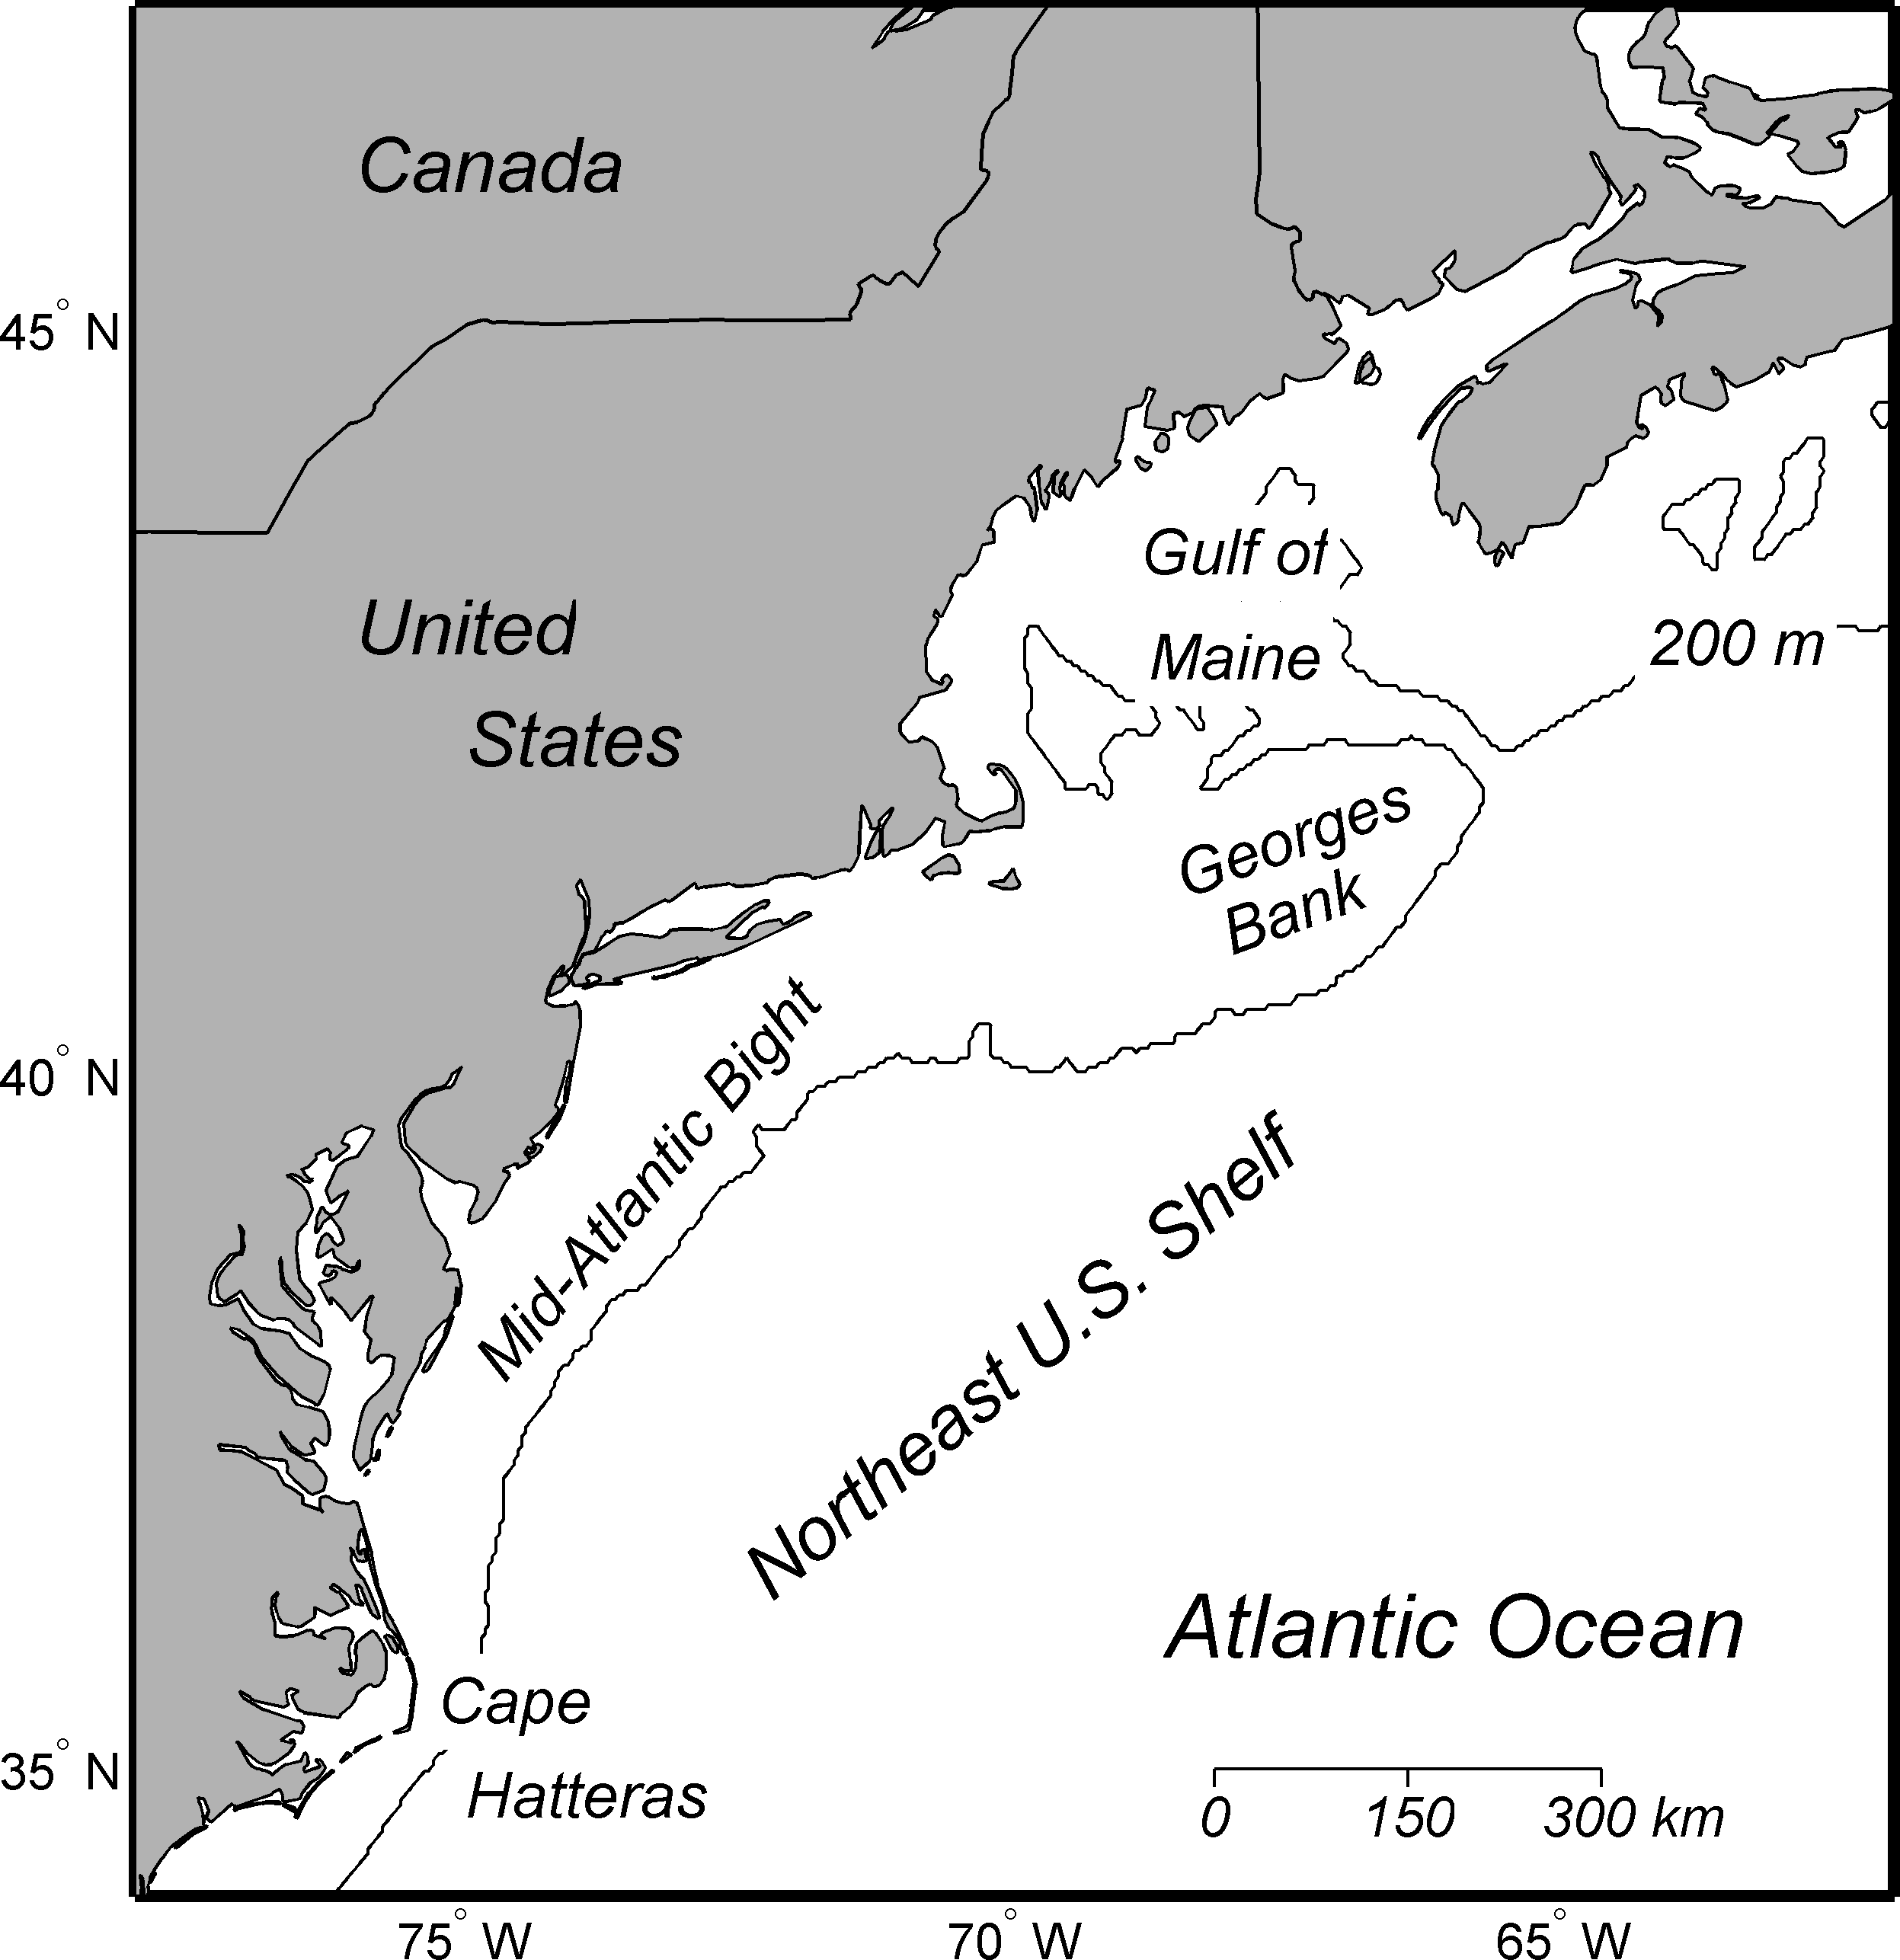
\includegraphics[width=34.64in]{images/journal.pone.0146756.g002} 

}

\caption{Map of Northeast U.S. Continental Shelf Large Marine Ecosystem from Hare et al. (\protect\hyperlink{ref-Hare2016}{2016}).}\label{fig:neusmap}
\end{figure}

\hypertarget{erddap}{%
\chapter{Data and Code Access}\label{erddap}}

\hypertarget{about}{%
\subsection{About}\label{about}}

The Technical Documentation for the State of the Ecosystem (SOE) reports is a \href{https://bookdown.org}{bookdown} document; hosted on the NOAA Northeast Fisheries Science Center (NEFSC) Ecosystems Dynamics and Assessment Branch \href{https://github.com/NOAA-EDAB}{Github page}, and developed in R. Derived data used to populate figures in this document are queried directly from the \href{https://github.com/NOAA-EDAB/ecodata}{ecodata} R package or the NEFSC \href{https://comet.nefsc.noaa.gov/erddap/info/index.html?page=1\&itemsPerPage=1000}{ERDDAP server}. ERDDAP queries are made using the R package \href{https://cran.r-project.org/web/packages/rerddap/vignettes/Using_rerddap.html}{rerddap}.

\hypertarget{accessing-data-and-build-code}{%
\subsection{Accessing data and build code}\label{accessing-data-and-build-code}}

In this technical documentation, we hope to shine a light on the processing and analytical steps involved to get from source data to final product. This means that whenever possible, we have included the code involved in source data extraction, processing, and analyses. We have also attempted to thoroughly describe all methods in place of or in supplement to provided code. Example plotting code for each indicator is presented in sections titled ``Plotting'', and these code chunks can be used to recreate the figures found in ecosystem reporting documents where each respective indicator was included\footnote{There are multiple R scripts sourced throughout this document in an attempt to keep code concise. These scripts include \href{https://github.com/NOAA-EDAB/tech-doc/blob/master/R/BasePlot_source.R}{BasePlot\_source.R}, \href{https://github.com/NOAA-EDAB/tech-doc/blob/master/R/GIS_source.R}{GIS\_source.R}, and \href{https://github.com/NOAA-EDAB/tech-doc/blob/master/R/get_erddap.R}{get\_erddap.R}. The scripts \texttt{BasePlot\_source.R} and \texttt{GIS\_source.R} refer to deprecated code used prior to the 2019 State of the Ecosystem reports. Indicators that were not included in reports after 2018 make use of this syntax, whereas newer indicators typically use \texttt{ggplot2} for plotting.}.

Source data for the derived indicators in this document are linked to in the text unless there are privacy concerns involved. In that case, it may be possible to access source data by reaching out to the Point of Contact associated with that data set. Derived data sets make up the majority of the indicators presented in ecosystem reporting documents, and these data sets are available for download through the \href{https://github.com/NOAA-EDAB/ecodata}{ecodata} R package.

\hypertarget{building-the-document}{%
\subsection{Building the document}\label{building-the-document}}

Start a local build of the SOE bookdown document by first cloning the project's associated \href{https://github.com/NOAA-EDAB/tech-doc}{git repository}. Next, if you would like to build a past version of the document, use \texttt{git\ checkout\ {[}version\_commit\_hash{]}} to revert the project to a past commit of interest, and set \texttt{build\_latest\ \textless{}-\ FALSE} in this \href{https://github.com/NOAA-EDAB/tech-doc/tree/master/R/stored_scripts/erddap_query_and_build_code.R}{code chunk}. This will ensure the project builds from a cached data set, and not the most updated versions present on the NEFSC ERDDAP server. Once the \texttt{tech-doc.Rproj} file is opened in RStudio, run \texttt{bookdown::serve\_book()} from the console to build the document.

\hypertarget{a-note-on-data-structures}{%
\subsubsection{A note on data structures}\label{a-note-on-data-structures}}

The majority of the derived time series used in State of the Ecosystem reports are in long format. This approach was taken so that all disparate data sets could be ``bound'' together for ease of use in our base plotting \href{(https://github.com/NOAA-EDAB/tech-doc/blob/master/R/BasePlot_source.R)}{functions}.

\hypertarget{aggroups}{%
\chapter{Aggregate Groups}\label{aggroups}}

\textbf{Description}: Mappings of species into aggregate group categories for different analyses

\textbf{Found in}: State of the Ecosystem - Gulf of Maine \& Georges Bank (2018, 2019, 2020), State of the Ecosystem - Mid-Atlantic (2018, 2019, 2020)

\textbf{Indicator category}: Synthesis of published information

\textbf{Contributor(s)}: Geret DePiper, Sarah Gaichas, Sean Hardison, Sean Lucey

\textbf{Data steward}: Sean Lucey \href{mailto:Sean.Lucey@noaa.gov}{\nolinkurl{Sean.Lucey@noaa.gov}}

\textbf{Point of contact}: Sean Lucey \href{mailto:Sean.Lucey@noaa.gov}{\nolinkurl{Sean.Lucey@noaa.gov}}

\textbf{Public availability statement}: Source data is available to the public (see Data Sources).

\hypertarget{methods}{%
\section{Methods}\label{methods}}

The State of the Ecosystem (SOE) reports are delivered to the New England Fishery Management Council (NEFMC) and Mid-Atlantic Fishery Management Council (MAFMC) to provide ecosystems context. To better understand that broader ecosystem context, many of the indicators are reported at an aggregate level rather than at a single species level. Species were assigned to an aggregate group following the classification scheme of Garrison and Link (\protect\hyperlink{ref-garrison2000dietary}{2000}) and Link et al. (\protect\hyperlink{ref-link2006EMAX}{2006}). Both works classified species into feeding guilds based on food habits data collected at the Northeast Fisheries Science Center (NEFSC). In 2017, the SOE used seven specific feeding guilds (plus an ``other'' category; Table \ref{tab:soe2017class}). These seven were the same guilds used in Garrison and Link (\protect\hyperlink{ref-garrison2000dietary}{2000}), which also distinguished ontogentic shifts in species diets.

For the purposes of the SOE, species were only assigned to one category based on the most prevalent size available to commercial fisheries. However, several of those categories were confusing to the management councils, so in 2018 those categories were simplified to five (plus ``other''; Table \ref{tab:soe2018class}) along the lines of Link et al. (\protect\hyperlink{ref-link2006EMAX}{2006}). In addition to feeding guilds, species managed by the councils have been identified. This is done to show the breadth of what a given council is responsible for within the broader ecosystem context.

In the 2020 report, squids were moved from planktivores to piscivores based on the majority of their diet being either fish or other squid.

\begin{table}

\caption{\label{tab:soe2017class}Aggregate groups use in 2017 SOE.  Classifications are based on @garrison2000dietary . \label{}}
\centering
\begin{tabular}[t]{ll}
\toprule
Feeding.Guild & Description\\
\midrule
Apex Predator & Top of the food chain\\
Piscivore & Fish eaters\\
Macrozoo-piscivore & Shrimp and small fish eaters\\
Macroplanktivore & Amphipod and shrimp eaters\\
Mesoplanktivore & Zooplankton eaters\\
\addlinespace
Benthivore & Bottom eaters\\
Benthos & Things that live on the bottom\\
Other & Things not classified above\\
\bottomrule
\end{tabular}
\end{table}

\begin{table}

\caption{\label{tab:soe2018class}Aggregate groups use since 2018 SOE.  Classifications are based on @link2006EMAX.}
\centering
\begin{tabular}[t]{ll}
\toprule
Feeding.Guild & Description\\
\midrule
Apex Predator & Top of the food chain\\
Piscivore & Fish eaters\\
Planktivore & Zooplankton eaters\\
Benthivore & Bottom eaters\\
Benthos & Things that live on the bottom\\
\addlinespace
Other & Things not classified above\\
\bottomrule
\end{tabular}
\end{table}

\hypertarget{data-sources}{%
\subsection{Data sources}\label{data-sources}}

In order to match aggregate groups with various data sources, a look-up table was generated which includes species' common names (COMNAME) along with their scientific names (SCINAME) and several species codes. SVSPP codes are used by the NEFSC Ecosystems Surveys Branch (ESB) in their fishery-independent Survey Database (SVDBS), while NESPP3 codes refer to the codes used by the Commercial Fisheries Database System (CFDBS) for fishery-dependent data. A third species code provided is the ITISSPP, which refers to species identifiers used by the Integrated Taxonomic Information System (ITIS). Digits within ITIS codes are hierarchical, with different positions in the identifier referring to higher or lower taxonomic levels. More information about the SVDBS, CFDBS, and ITIS species codes are available in the links provided below.

Management responsibilities for different species are listed under the column ``Fed.managed'' (NEFMC, MAFMC, or JOINT for jointly managed species). More information about these species is available on the FMC websites listed below. Species groupings listed in the ``NEIEA'' column were developed for presentation on the Northeast Integrated Ecosystem Assessment (NE-IEA) website. These groupings are based on EMAX groupings (Link et al. \protect\hyperlink{ref-link2006EMAX}{2006}), but were adjusted based on conceptual models developed for the NE-IEA program that highlight focal components in the Northeast Large Marine Ecosystem (i.e.~those components with the largest potential for perturbing ecosystem dynamics). NE-IEA groupings were further simplified to allow for effective communication through the NE-IEA website.

\hypertarget{supplemental-information}{%
\subsubsection{Supplemental information}\label{supplemental-information}}

See the following links for more information regarding the NEFSC ESB Bottom Trawl Survey, CFDBS, and ITIS:

\begin{itemize}
\tightlist
\item
  \url{https://www.itis.gov/}~\\
\item
  \url{https://inport.nmfs.noaa.gov/inport/item/22561}~\\
\item
  \url{https://inport.nmfs.noaa.gov/inport/item/22560}~\\
\item
  \url{https://inport.nmfs.noaa.gov/inport/item/27401}
\end{itemize}

More information about the NE-IEA program is available \href{http://integratedecosystemassessment.noaa.gov}{here}.

More information about the New Engalnd Fisheries Management Council is available \href{https://www.nefmc.org/}{here}.

More information about the Mid-Atlantic Fisheries Management Council is available \href{http://www.mafmc.org/}{here}.

\hypertarget{data-extraction}{%
\subsection{Data extraction}\label{data-extraction}}

Species lists are pulled from SVDBS and CFDBS. They are merged using the ITIS code. Classifications from Garrison and Link (Garrison and Link \protect\hyperlink{ref-garrison2000dietary}{2000}) and Link et al.~(Link et al. \protect\hyperlink{ref-link2006EMAX}{2006}) are added manually. The R code used in the extraction process can be found \href{https://github.com/slucey/RSurvey/blob/master/Species_list.R}{here}.

\hypertarget{annual-sst-cycles}{%
\chapter{Annual SST Cycles}\label{annual-sst-cycles}}

\textbf{Description}: Annual SST Cycles

\textbf{Found in}: State of the Ecosystem - Gulf of Maine \& Georges Bank (2018), State of the Ecosystem - Mid-Atlantic (2018)

\textbf{Indicator category}: Database pull with analysis

\textbf{Contributor(s)}: Sean Hardison, Vincent Saba

\textbf{Data steward}: Kimberly Bastille, \href{mailto:kimberly.bastille@noaa.gov}{\nolinkurl{kimberly.bastille@noaa.gov}}

\textbf{Point of contact}: Kimberly Bastille, \href{mailto:kimberly.bastille@noaa.gov}{\nolinkurl{kimberly.bastille@noaa.gov}}

\textbf{Public availability statement}: Source data are available \href{https://www.esrl.noaa.gov/psd/data/gridded/data.noaa.oisst.v2.highres.html}{here}.

\hypertarget{methods-1}{%
\section{Methods}\label{methods-1}}

\hypertarget{data-sources-1}{%
\subsection{Data sources}\label{data-sources-1}}

Data for annual sea surface tempature (SST) cycles were derived from the NOAA optimum interpolation sea surface temperature (OISST) high resolution dataset (\href{https://www.esrl.noaa.gov/psd/data/gridded/data.noaa.oisst.v2.highres.html}{NOAA OISST V2 dataset}) provided by NOAA's Earth System Research Laboratory's Physical Sciences Devision, Boulder, CO. The data extend from 1981 to present, and provide a 0.25° x 0.25° global grid of SST measurements (Reynolds et al. \protect\hyperlink{ref-Reynolds2007}{2007}). Gridded SST data were masked according to the extent of Ecological Production Units (EPU) in the Northeast Large Marine Ecosystem (NE-LME) (See \href{https://github.com/NOAA-EDAB/tech-doc/tree/master/gis}{``EPU\_Extended'' shapefiles}).

\hypertarget{data-extraction-1}{%
\subsection{Data extraction}\label{data-extraction-1}}

Daily mean sea surface temperature data for 2017 and for each year during the period of 1981-2012 were downloaded from the NOAA \href{https://www.esrl.noaa.gov/psd/data/gridded/data.noaa.oisst.v2.highres.html}{OI SST V2 site} to derive the long-term climatological mean for the period. The use of a 30-year climatological reference period is a standard procedure for metereological observing (WMO \protect\hyperlink{ref-WMO2017}{2017}). These reference periods serve as benchmarks for comparing current or recent observations, and for the development of standard anomaly data sets. The reference period of 1982-2012 was chosen to be consistent with previous versions of the State of the Ecosystem report.

R code used in extraction and processing can be found \href{https://github.com/NOAA-EDAB/tech-doc/blob/master/R/stored_scripts/annual_sst_cycles_extraction_and_processing.R}{here}

\hypertarget{data-analysis}{%
\subsection{Data analysis}\label{data-analysis}}

We calculated the long-term mean and standard deviation of SST over the period of 1982-2012 for each EPU, as well as the daily mean for 2017.

R code used for analysis and plotting can be found \href{https://github.com/NOAA-EDAB/tech-doc/blob/master/R/stored_scripts/annual_sst_cycles_analysis_and_plotting.R}{here}

\begin{figure}

{\centering 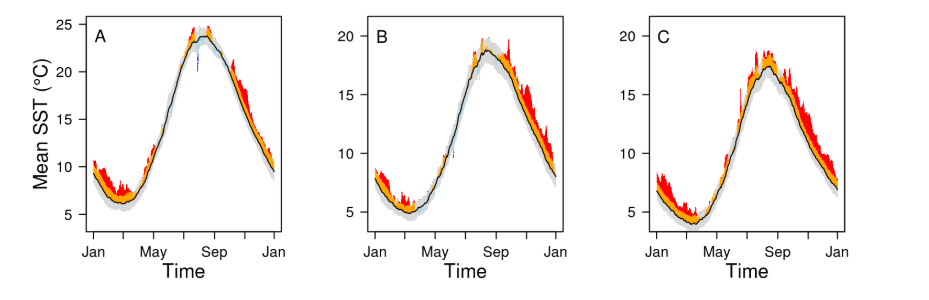
\includegraphics[width=12.9in]{/home/travis/build/NOAA-EDAB/tech-doc/images/annual_SST_cycle_plot} 

}

\caption{Long-term mean SSTs for the Mid-Atlantic Bight (A), Georges Bank (B), and Gulf of Maine (C). Orange and cyan shading show where the 2017 daily SST values were above or below the long-term mean respectively; red and dark blue shades indicate days when the 2017 mean exceeded +/- 1 standard deviation from the long-term mean.}\label{fig:unnamed-chunk-1}
\end{figure}

\hypertarget{aquaculture}{%
\chapter{Aquaculture}\label{aquaculture}}

\textbf{Description}: Aquaculture indicators

\textbf{Found in}: State of the Ecosystem - Gulf of Maine \& Georges Bank (2017, 2018), State of the Ecosystem - Mid-Atlantic (2017, 2018, 2019)

\textbf{Indicator category}: Synthesis of published information

\textbf{Contributor(s)}: Sean Hardison, Lisa Calvo, Karl Roscher

\textbf{Data steward}: Kimberly Bastille \href{mailto:kimberly.bastille@noaa.gov}{\nolinkurl{kimberly.bastille@noaa.gov}}

\textbf{Point of contact}: Kimberly Bastille \href{mailto:kimberly.bastille@noaa.gov}{\nolinkurl{kimberly.bastille@noaa.gov}}

\textbf{Public availability statement}: Source data are publicly available in referenced reports, and are also available for download \href{https://comet.nefsc.noaa.gov/erddap/tabledap/aquaculture_soe_v1.html}{here}.

\hypertarget{methods-2}{%
\section{Methods}\label{methods-2}}

Aquaculture data included in the State of the Ecosystem (SOE) report were time series of number of oysters sold in Virginia, Maryland, and New Jersey.

\hypertarget{data-sources-2}{%
\subsection{Data sources}\label{data-sources-2}}

Virginia oyster harvest data are collected from mail and internet-based surveys of active oyster aquaculture operations on both sides of the Chesapeake Bay, which are then synthesized in an annual report (Hudson \protect\hyperlink{ref-Hudson2017a}{2017}). In Maryland, shellfish aquaculturists are required to report their monthly harvests to the Maryland Department of Natural Resources (MD-DNR). The MD-DNR then aggregates the harvest data for release in the Maryland Aquaculture Coordinating Council Annual Report (ACC \protect\hyperlink{ref-ACC2017}{2017}), from which data were collected. Similar to Virginia, New Jersey releases annual reports synthesizing electronic survey results from lease-holding shellfish growers. Data from New Jersey reflects cage reared oysters grown from hatchery seed (Calvo \protect\hyperlink{ref-Calvo2017}{2017}).

\hypertarget{data-extraction-2}{%
\subsection{Data extraction}\label{data-extraction-2}}

Data were collected directly from state aquaculture reports. Oyster harvest data in MD was reported in bushels which were then converted to individual oysters by an estimate of 300 oysters bushel\(^{-1}\). View processing code for this indicator \href{https://github.com/NOAA-EDAB/ecodata/blob/master/data-raw/get_aquaculture.R}{here}.

\hypertarget{data-analysis-1}{%
\subsection{Data analysis}\label{data-analysis-1}}

No data analyses occurred for this indicator.

\hypertarget{data-processing}{%
\subsection{Data processing}\label{data-processing}}

Aquaculture data were formatted for inclusion in the \texttt{ecodata} R package using the code found \href{https://github.com/NOAA-EDAB/ecodata/blob/master/data-raw/get_aquaculture.R}{here}.

\hypertarget{plotting}{%
\subsection{Plotting}\label{plotting}}

Code for plotting data included in the State of the Ecosystem report can be found \href{https://github.com/NOAA-EDAB/ecodata/blob/master/chunk-scripts/human_dimensions.Rmd-oyster-aqua.R}{here}.

\begin{figure}

{\centering 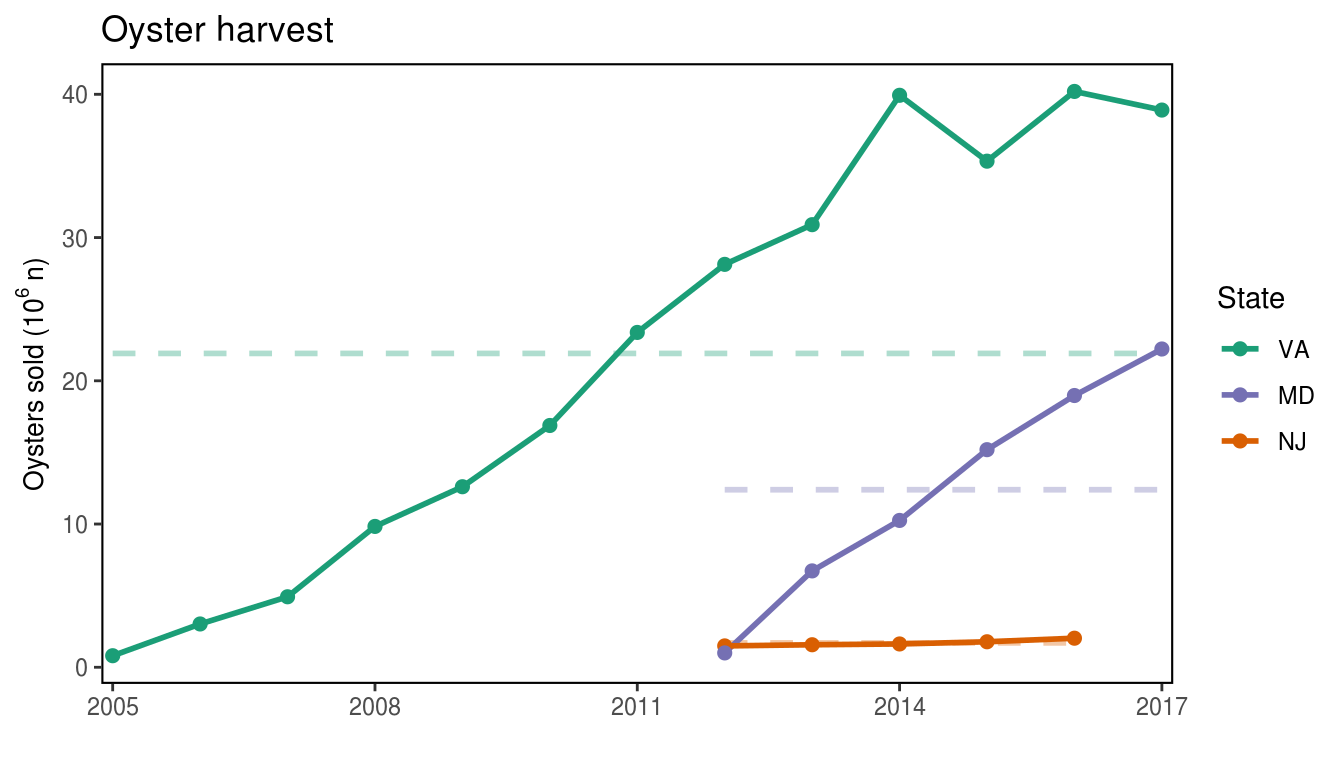
\includegraphics{/home/travis/build/NOAA-EDAB/tech-doc/images/unnamed-chunk-2-1} 

}

\caption{Oyster aquaculture production in terms of number of oysters sold from Virginia, Maryland, and New Jersey.}\label{fig:unnamed-chunk-2}
\end{figure}

\hypertarget{bennet-indicator}{%
\chapter{Bennet Indicator}\label{bennet-indicator}}

\textbf{Description}: Bennet Indicator

\textbf{Found in}: State of the Ecosystem - Gulf of Maine \& Georges Bank (2018, 2019, 2020), State of the Ecosystem - Mid-Atlantic (2018, 2019, 2020)

\textbf{Indicator category}: Database pull with analysis

\textbf{Contributor(s)}: John Walden

\textbf{Data steward}:Kimberly Bastille, \href{mailto:kimberly.bastille@noaa.gov}{\nolinkurl{kimberly.bastille@noaa.gov}}

\textbf{Point of contact}: John Walden, \href{mailto:john.walden@noaa.gov}{\nolinkurl{john.walden@noaa.gov}}

\textbf{Public availability statement}: Derived CFDBS data are available for this analysis (see \protect\hyperlink{comdat}{Comland}).

\hypertarget{methods-3}{%
\section{Methods}\label{methods-3}}

\hypertarget{data-sources-3}{%
\subsection{Data sources}\label{data-sources-3}}

Data used in the Bennet Indicator were derived from the Comland data set; a processed subset of the Commercial Fisheries Database System (CFDBS). The derived Comland data set is available for download \href{https://comet.nefsc.noaa.gov/erddap/tabledap/group_landings_soe_v1.html}{here}.

\hypertarget{data-extraction-3}{%
\subsection{Data extraction}\label{data-extraction-3}}

For information regarding processing of CFDBS, please see \protect\hyperlink{comdat}{Comland} methods. The Comland dataset containing seafood landings data was subsetted to US landings after 1964 where revenue was \(\ge\) 0 for each Ecological Production Unit (i.e.~Mid-Atlantic Bight, Georges Bank, and Gulf of Maine). Each EPU was run in an individual R script, and the code specific to Georges Bank is shown {[}here{]}(.

\hypertarget{data-analysis-2}{%
\subsection{Data analysis}\label{data-analysis-2}}

Revenue earned by harvesting resources from a Large Marine Ecosystem (LME) at time \emph{t} is a function of both the quantity landed of each species and the prices paid for landings. Changes in revenue between any two years depends on both prices and quantities in each year, and both may be changing simultaneously. For example, an increase in the harvest of higher priced species, such as scallops can lead to an overall increase in total revenue from an LME between time periods even if quantities landed of other species decline. Although measurement of revenue change is useful, the ability to see what drives revenue change, whether it is changing harvest levels, the mix of species landed, or price changes provides additional valuable information. Therefore, it is useful to decompose revenue change into two parts, one which is due to changing quantities (or volumes), and a second which is due to changing prices. In an LME, the quantity component will yield useful information about how the species mix of harvests are changing through time.

A Bennet indicator (BI) is used to examine revenue change between 1964 and 2015 for two major LME regions. It is composed of a volume indicator (VI), which measures changes in quantities, and a price indicator (PI) which measures changes in prices. The Bennet (1920) indicator (BI) was first used to show how a change in social welfare could be decomposed into a sum of a price and quantity change indicator (Cross and Färe \protect\hyperlink{ref-Cross2009}{2009}). It is called an indicator because it is based on differences in value between time periods, rather than ratios, which are referred to as indices. The BI is the indicator equivalent of the more popular Fisher index (Balk \protect\hyperlink{ref-Balk2010}{2010}), and has been used to examine revenue changes in Swedish pharmacies, productivity change in U.S. railroads (Lim and Lovell \protect\hyperlink{ref-lim2009}{2009}), and dividend changes in banking operations (Grifell-Tatjé and Lovell \protect\hyperlink{ref-Grifell-Tatje2004}{2004}). An attractive feature of the BI is that the overall indicator is equal to the sum of its subcomponents (Balk \protect\hyperlink{ref-Balk2010}{2010}). This allows one to examine what component of overall revenue is responsible for change between time periods. This allows us to examine whether changing quantities or prices of separate species groups are driving revenue change in each EPU between 1964 and 2015.

Revenue in a given year for any species group is the product of quantity landed times price, and the sum of revenue from all groups is total revenue from the LME. In any year, both prices and quantities can change from prior years, leading to total revenue change. At time t, revenue (R) is defined as \[R^{t} = \sum_{j=1}^{J}p_{j}^{t}y_{j}^{t},\]
where \(p_{j}\) is the price for species group \(j\), and \(y_{j}\) is the quantity landed of species group \(j\). Revenue change between any two time periods, say \(t+1\) and \(t\), is then \(R^{t+1}-R^{t}\), which can also be expressed as:
\[\Delta R = \sum_{j=1}^{J}p_{j}^{t+1}y_{j}^{t+1}-\sum_{j=1}^{J}p_{j}^{t}y_{j}^{t}.\]
This change can be decomposed further, yielding a VI and PI. The VI is calculated using the following formula (Georgianna, Lee, and Walden \protect\hyperlink{ref-Georgianna2017}{2017}):

\[VI = \frac{1}{2}(\sum_{j=1}^{J}p_{j}^{t+1}y_{j}^{t+1} - \sum_{j=1}^{J}p_{j}^{t+1}y_{j}^{t} + \sum_{j=1}^{J}p_{j}^{t}y_{j}^{t+1} - \sum_{j=1}^{J}p_{j}^{t}y_{j}^{t})\]
The price indicator (PI) is calculated as follows:
\[PI = \frac{1}{2}(\sum_{j=1}^{J}y_{j}^{t+1}p_{j}^{t+1} - \sum_{j=1}^{J}y_{j}^{t+1}p_{j}^{t} + \sum_{j=1}^{J}y_{j}^{t}p_{j}^{t+1} - \sum_{j=1}^{J}y_{j}^{t}p_{j}^{t})\]
Total revenue change between time \(t\) and \(t+1\) is the sum of the VI and PI. Since revenue change is being driven by changes in the individual prices and quantities landed of each species group, changes at the species group level can be examined separately by taking advantage of the additive property of the indicator. For example, if there are five different species groups, the sum of the VI for each group will equal the overall VI, and the sum of the PI for each group will equal the overall PI.

\hypertarget{data-processing-1}{%
\subsection{Data processing}\label{data-processing-1}}

Bennet indicator time series were formatted for inclusion in the \texttt{ecodata} R package using the R code found \href{https://raw.githubusercontent.com/NOAA-EDAB/ecodata/master/data-raw/get_bennet.R}{here}.

\hypertarget{plotting-1}{%
\subsection{Plotting}\label{plotting-1}}

Code for plotting the bennet indicator can be found \href{https://github.com/NOAA-EDAB/ecodata/blob/master/chunk-scripts/human_dimensions.Rmd-bennet.R}{here}.

\begin{figure}
\centering
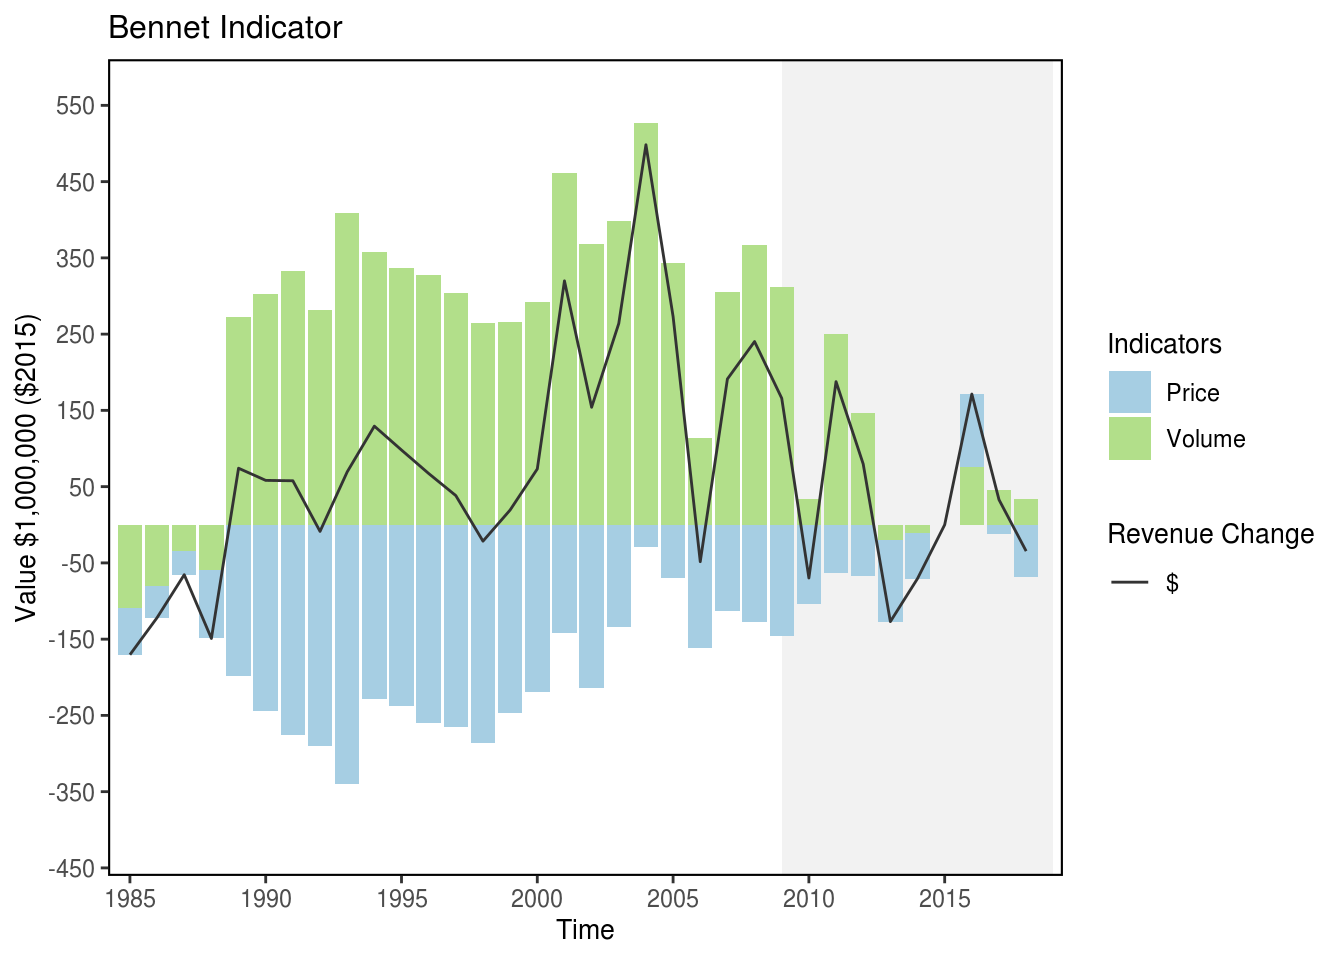
\includegraphics{/home/travis/build/NOAA-EDAB/tech-doc/images/unnamed-chunk-3-1.pdf}
\caption{\label{fig:unnamed-chunk-3}Revenue change from the long-term mean in 2015 dollars (black), Price (PI), and Volume Indicators (VI) for commercial landings in the Mid-Atlantic.}
\end{figure}

\hypertarget{bottom-temperatures}{%
\chapter{Bottom temperatures}\label{bottom-temperatures}}

\textbf{Description}: Time series of annual in situ bottom temperatures on the Northeast Continental Shelf.

\textbf{Indicator category}: Extensive analysis; not yet published
Found in: State of the Ecosystem - Gulf of Maine \& Georges Bank (2019, 2020); State of the Ecosystem - Mid-Atlantic Bight (2019, 2020)

\textbf{Contributor(s)}: Paula Fratantoni, \href{mailto:paula.fratantoni@noaa.gov}{\nolinkurl{paula.fratantoni@noaa.gov}}

\textbf{Data steward}: Kimberly Bastille, \href{mailto:kimberly.bastille@noaa.gov}{\nolinkurl{kimberly.bastille@noaa.gov}}

\textbf{Point of contact}: Paula Fratantoni, \href{mailto:paula.fratantoni@noaa.gov}{\nolinkurl{paula.fratantoni@noaa.gov}}

\textbf{Public availability statement}: Source data are publicly available at \url{ftp://ftp.nefsc.noaa.gov/pub/hydro/matlab_files/yearly} and in the World Ocean Database housed at \url{http://www.nodc.noaa.gov/OC5/SELECT/dbsearch/dbsearch.html} under institute code number 258.

\hypertarget{methods-4}{%
\section{Methods}\label{methods-4}}

\hypertarget{data-sources-4}{%
\subsection{Data sources}\label{data-sources-4}}

The bottom temperature index incorporates near-bottom temperature measurements collected on Northeast Fisheries Science Center (NEFSC) surveys between 1977-present. Early measurements were made using surface bucket samples, mechanical bathythermographs and expendable bathythermograph probes, but by 1991 the CTD -- an acronym for conductivity temperature and depth -- became standard equipment on all NEFSC surveys. Near-bottom refers to the deepest observation at each station that falls within 10 m of the reported water depth. Observations encompass the entire continental shelf area extending from Cape Hatteras, NC to Nova Scotia, Canada, inclusive of the Gulf of Maine and Georges Bank.

\hypertarget{data-extraction-4}{%
\subsection{Data extraction}\label{data-extraction-4}}

While all processed hydrographic data are archived in an Oracle database (OCDBS), we work from Matlab-formatted files stored locally.

\hypertarget{data-analysis-3}{%
\subsection{Data analysis}\label{data-analysis-3}}

Ocean temperature on the Northeast U.S. Shelf varies significantly on seasonal timescales. Any attempt to resolve year-to-year changes requires that this seasonal variability be quantified and removed to avoid bias. This process is complicated by the fact that NEFSC hydrographic surveys conform to a random stratified sampling design meaning that stations are not repeated at fixed locations year after year so that temperature variability cannot be assessed at fixed station locations. Instead, we consider the variation of the average bottom temperature within four \protect\hyperlink{epu}{Ecological Production Units} (EPUs): Middle Atlantic Bight, Georges Bank, Gulf of Maine and Scotian Shelf. Within each EPU, ocean temperature observations are extracted from the collection of measurements made within 10 m of the bottom on each survey and an area-weighted average temperature is calculated. The result of this calculation is a timeseries of regional average near-bottom temperature having a temporal resolution that matches the survey frequency in the database. Anomalies are subsequently calculated relative to a reference annual cycle, estimated using a multiple linear regression model to fit an annual harmonic (365-day period) to historical regional average temperatures from 1981-2010. The curve fitting technique to formulate the reference annual cycle follows the methodologies outlined by Mountain (\protect\hyperlink{ref-mountain1991}{1991}). The reference period was chosen because it is the standard climatological period adopted by the World Meteorological Organization. The resulting anomaly time series represents the difference between the time series of regional mean temperatures and corresponding reference temperatures predicted by a reference annual cycle for the same time of year. Finally, a reference annual average temperature (calculated as the average across the reference annual cycle) is added back into the anomaly timeseries to convert temperature anomalies back to ocean bottom temperature.

\hypertarget{data-processing-2}{%
\subsection{Data processing}\label{data-processing-2}}

Derived bottom temperature data were formatted for inclusion in the \texttt{ecodata} R package using the R code found \href{https://github.com/NOAA-EDAB/ecodata/blob/master/data-raw/get_bottom_temp.R}{here}.

\hypertarget{plotting-2}{%
\subsection{Plotting}\label{plotting-2}}

Code for plotting Georges Bank and Gulf of Maine bottom temperature time series can be found \href{https://github.com/NOAA-EDAB/ecodata/blob/master/chunk-scripts/LTL.Rmd-MAB-bot-temp.R}{here}.

\begin{figure}
\centering
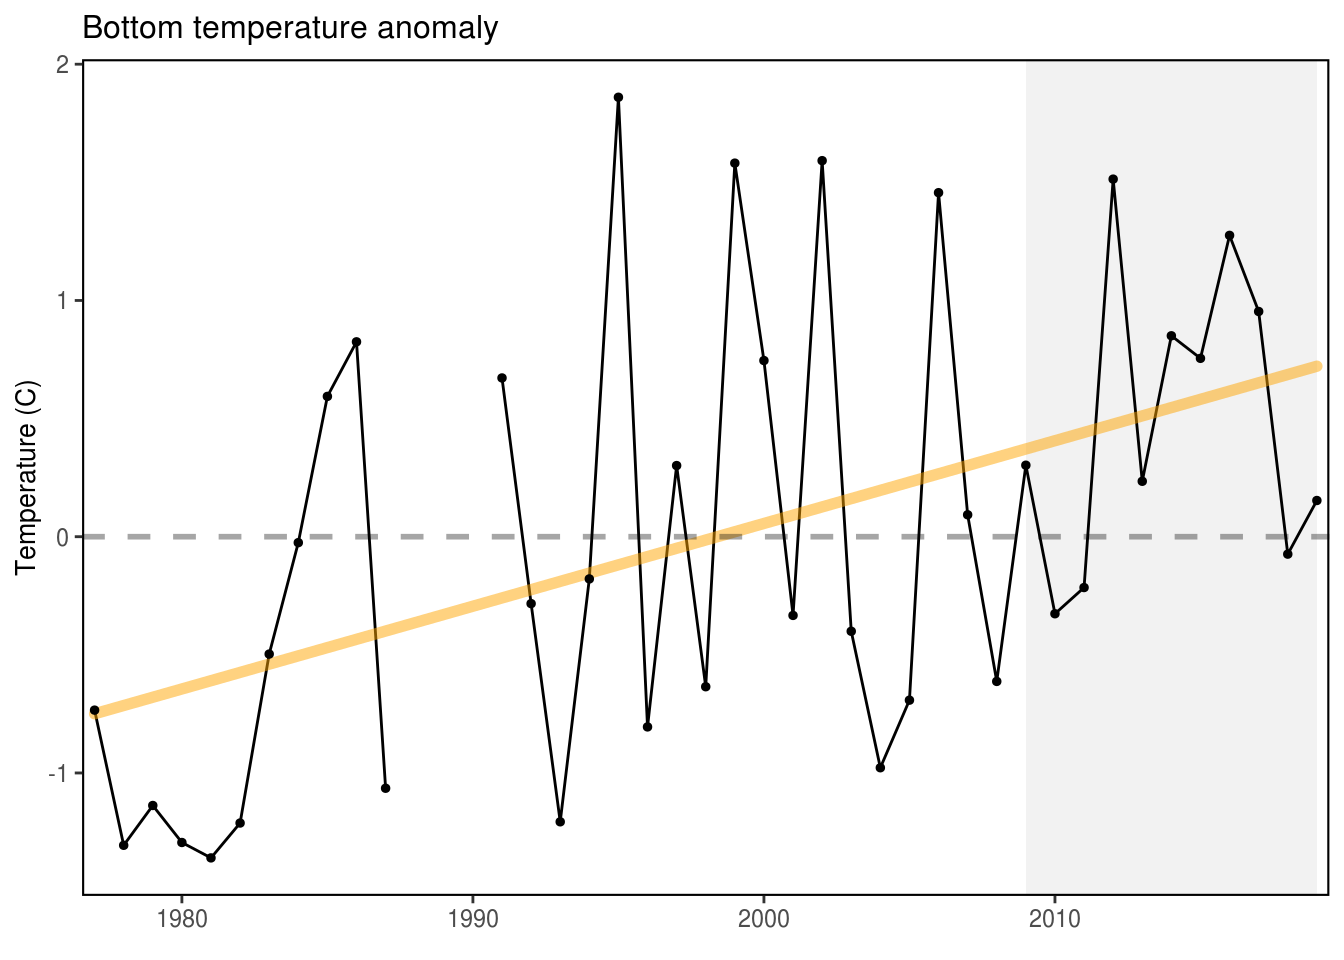
\includegraphics{/home/travis/build/NOAA-EDAB/tech-doc/images/unnamed-chunk-4-1.pdf}
\caption{\label{fig:unnamed-chunk-4}Mid-Atlantic annual bottom temperature anomalies.}
\end{figure}

\hypertarget{catch-and-fleet-diversity}{%
\chapter{Catch and Fleet Diversity}\label{catch-and-fleet-diversity}}

\textbf{Description}: Permit-level species diversity and Council-level fleet diversity.

\textbf{Found in}: State of the Ecosystem - Gulf of Maine \& Georges Bank (2018), State of the Ecosystem - Mid-Atlantic (2018)

\textbf{Indicator category}: Database pull with analysis; Published methods

\textbf{Contributor(s)}: Geret DePiper, Min-Yang Lee

\textbf{Data steward}: Geret DePiper, \href{mailto:geret.depiper@noaa.gov}{\nolinkurl{geret.depiper@noaa.gov}}

\textbf{Point of contact}: Geret DePiper, \href{mailto:geret.depiper@noaa.gov}{\nolinkurl{geret.depiper@noaa.gov}}

\textbf{Public availability statement}: Source data is not publicly availabe due to PII restrictions. Derived time series are available for download \href{https://comet.nefsc.noaa.gov/erddap/tabledap/comm_data_soe_v1.html}{here}.

\hypertarget{methods-5}{%
\section{Methods}\label{methods-5}}

Diversity estimates have been developed to understand whether specialization, or alternatively stovepiping, is occurring in fisheries of the Northeastern Large Marine Ecosystem. We use the average effective Shannon indices for species revenue at the permit level, for all permits landing any amount of \href{https://www.nefmc.org/}{NEFMC} or \href{http://www.mafmc.org/}{MAFMC} Fishery Management Plan (FMP) species within a year (including both Monkfish and Spiny Dogfish). We also use the effective Shannon index of fleet revenue diversity and count of active fleets to assess the extent to which the distribution of fishing changes across fleet segments.

\hypertarget{data-sources-5}{%
\subsection{Data sources}\label{data-sources-5}}

Data for these diversity estimates comes from a variety of sources, including the
Commercial Fishery Dealer Database, Vessel Trip Reports, Clam logbooks, vessel characteristics from Permit database, WPU series producer price index. These data are typically not available to the public.

\hypertarget{data-extraction-5}{%
\subsection{Data extraction}\label{data-extraction-5}}

The following describes both the permit-level species and fleet diversity data generation. Price data was extracted from the Commercial Fishery Dealer database (CFDERS) and linked to Vessel Trip Reports by a heirarchical matching algorithm that matched date and port of landing at its highest resolution. Code used in these analyses is available upon request.

Output data was then matched to vessel characteristics from the VPS VESSEL data set. For the permit-level estimate, species groups are based off of a slightly refined NESPP3 code (Table \ref{tab:spp-groupings}), defined in the data as ``myspp'', which is further developed in the script to rectify inconsistencies in the data.

\begingroup\fontsize{8}{10}\selectfont

\begin{longtabu} to \linewidth {>{\raggedright}X>{\raggedleft}X>{\raggedright}X>{\raggedright}X}
\caption{\label{tab:spp-groupings}Species grouping}\\
\toprule
Group & NESPP3 & Common Name & Scientific Name\\
\midrule
\endfirsthead
\caption[]{\label{tab:spp-groupings}Species grouping \textit{(continued)}}\\
\toprule
Group & NESPP3 & Common Name & Scientific Name\\
\midrule
\endhead
\
\endfoot
\bottomrule
\endlastfoot
 & 470 & ALBACORE & THUNNUS ALALUNGA\\
\cmidrule{2-4}
 & 494 & ATLANTIC SHARPNOSE SHARK & RHIZOPRIONODON TERRAENOVAE\\
\cmidrule{2-4}
 & 354 & BIGEYE THRESHER SHARK & ALOPIAS SUPERCILIOSUS\\
\cmidrule{2-4}
 & 469 & BIGEYE TUNA & THUNNUS OBESUS\\
\cmidrule{2-4}
 & 487 & BLACKTIP SHARK & CARCHARHINUS LIMBATUS\\
\cmidrule{2-4}
 & 493 & BLUE SHARK & PRIONACE GLAUCA\\
\cmidrule{2-4}
 & 467 & BLUEFIN TUNA & THUNNUS THYNNUS\\
\cmidrule{2-4}
 & 468 & LITTLE TUNNY & EUTHYNNUS ALLETTERATUS\\
\cmidrule{2-4}
 & 358 & LONGFIN MAKO & ISURUS PAUCUS\\
\cmidrule{2-4}
 & 481 & PORBEAGLE SHARK & LAMNA NASUS\\
\cmidrule{2-4}
 & 349 & SAND TIGER & CARCHARIAS TAURUS\\
\cmidrule{2-4}
 & 482 & SANDBAR SHARK & CARCHARHINUS PLUMBEUS\\
\cmidrule{2-4}
 & 359 & SHARK,UNC & CHONDRICHTHYES\\
\cmidrule{2-4}
 & 355 & SHORTFIN MAKO & ISURUS OXYRINCHUS\\
\cmidrule{2-4}
 & 466 & SKIPJACK TUNA & KATSUWONUS PELAMIS\\
\cmidrule{2-4}
 & 432 & SWORDFISH & XIPHIAS GLADIUS\\
\cmidrule{2-4}
 & 353 & THRESHER SHARK & ALOPIAS VULPINUS\\
\cmidrule{2-4}
 & 491 & TIGER SHARK & GALEOCERDO CUVIER\\
\cmidrule{2-4}
\multirow{-19}{*}{\raggedright\arraybackslash Highly Migratory Species} & 471 & YELLOWFIN TUNA & THUNNUS ALBACARES\\
\cmidrule{1-4}
 & 11 & GOOSEFISH & LOPHIUS AMERICANUS\\
\cmidrule{2-4}
\multirow{-2}{*}{\raggedright\arraybackslash Monkfish in Mid-Atlantic Waters} & 12 & GOOSEFISH & LOPHIUS AMERICANUS\\
\cmidrule{1-4}
Atlantic Scallops & 800 & SEA SCALLOP & PLACOPECTEN MAGELLANICUS\\
\cmidrule{1-4}
 & 737 & MANTIS SHRIMP UNCL & STOMATOPODA\\
\cmidrule{2-4}
 & 737 & MANTIS SHRIMPS & STOMATOPODA\\
\cmidrule{2-4}
 & 736 & NORTHERN SHRIMP & PANDALUS BOREALIS\\
\cmidrule{2-4}
 & 738 & SHRIMP,ATLANTIC \& GULF,BROWN & PANAEIDAE\\
\cmidrule{2-4}
\multirow{-5}{*}{\raggedright\arraybackslash Shrimp} & 735 & SHRIMP,UNC (CARIDEA) & CARIDEA\\
\cmidrule{1-4}
 & 368 & BARNDOOR SKATE & DIPTURUS LAEVIS\\
\cmidrule{2-4}
 & 372 & CLEARNOSE SKATE & RAJA EGLANTERIA\\
\cmidrule{2-4}
 & 366 & LITTLE SKATE & LEUCORAJA ERINACEA\\
\cmidrule{2-4}
 & 365 & OCELLATE SKATES & RAJA\\
\cmidrule{2-4}
 & 365 & SKATES & RAJIDAE\\
\cmidrule{2-4}
 & 373 & SKATES,LITTLE/WINTER MIXED & LEUCORAJA\\
\cmidrule{2-4}
 & 369 & SMOOTH SKATE & MALACORAJA SENTA\\
\cmidrule{2-4}
 & 370 & THORNY SKATE & AMBLYRAJA RADIATA\\
\cmidrule{2-4}
\multirow{-9}{*}{\raggedright\arraybackslash Skates} & 367 & WINTER SKATE & LEUCORAJA OCELLATA\\
\cmidrule{1-4}
Herring & 168 & ATLANTIC HERRING & CLUPEA HARENGUS\\
\cmidrule{1-4}
Ocean Quahog & 754 & OCEAN QUAHOG & ARCTICA ISLANDICA\\
\cmidrule{1-4}
Surf Clam & 769 & ATLANTIC SURFCLAM & SPISULA SOLIDISSIMA\\
\cmidrule{1-4}
 & 444 & BLUELINE TILEFISH & CAULOLATILUS MICROPS\\
\cmidrule{2-4}
 & 445 & SAND TILEFISH & MALACANTHUS PLUMIERI\\
\cmidrule{2-4}
 & 446 & TILEFISH & LOPHOLATILUS CHAMAELEONTICEPS\\
\cmidrule{2-4}
\multirow{-4}{*}{\raggedright\arraybackslash Tilefish} & 447 & TILEFISH,UNC & MALACANTHIDAE\\
\cmidrule{1-4}
 & 335 & BLACK SEA BASS & CENTROPRISTIS STRIATA\\
\cmidrule{2-4}
\multirow{-2}{*}{\raggedright\arraybackslash Fluke \& Black Seabass} & 121 & SUMMER FLOUNDER & PARALICHTHYS DENTATUS\\
\cmidrule{1-4}
 & 51 & BUTTERFISH & PEPRILUS TRIACANTHUS\\
\cmidrule{2-4}
 & 152 & RED HAKE & UROPHYCIS CHUSS\\
\cmidrule{2-4}
\multirow{-3}{*}{\raggedright\arraybackslash Butterfish \& Hake} & 509 & SILVER HAKE & MERLUCCIUS BILINEARIS\\
\cmidrule{1-4}
Bluefish in Mid-Atlantic Waters & 23 & BLUEFISH & POMATOMUS SALTATRIX\\
\cmidrule{1-4}
Spiny Dogfish & 352 & SPINY DOGFISH & SQUALUS ACANTHIAS\\
\cmidrule{1-4}
Northern Shortfin Squid & 802 & NORTHERN SHORTFIN SQUID & ILLEX ILLECEBROSUS\\
\cmidrule{1-4}
American Lobster & 727 & AMERICAN LOBSTER & HOMARUS AMERICANUS\\
\cmidrule{1-4}
Longfin Squid & 801 & LONGFIN SQUID & LOLIGO PEALEII\\
\cmidrule{1-4}
Menhaden & 221 & MENHADEN & BREVOORTIA\\
\cmidrule{1-4}
Offshore Hake & 508 & OFFSHORE HAKE & MERLUCCIUS ALBIDUS\\
\cmidrule{1-4}
Scup in Mid-Atlantic Waters & 329 & SCUP & STENOTOMUS CHRYSOPS\\
\cmidrule{1-4}
Windowpane Flounder in New England Waters & 125 & WINDOWPANE & SCOPHTHALMUS AQUOSUS\\
\cmidrule{1-4}
Ocean Pout in New England Waters & 250 & OCEAN POUT & ZOARCES AMERICANUS\\
\cmidrule{1-4}
Wolffish & 512 & ATLANTIC WOLFFISH & ANARHICHAS LUPUS\\
\cmidrule{1-4}
Winter Flounder in Mid-Atlantic Waters & 120 & WINTER FLOUNDER & PSEUDOPLEURONECTES AMERICANUS\\
\cmidrule{1-4}
Yellowtail Flounder in Mid-Atlantic Waters & 123 & YELLOWTAIL FLOUNDER & LIMANDA FERRUGINEA\\
\cmidrule{1-4}
Unclassified Hake & 155 & Unclassified Hake & \\
\cmidrule{1-4}
White Hake in Mid-Atlantic Waters & 153 & WHITE HAKE & UROPHYCIS TENUIS\\
\cmidrule{1-4}
 & 23 & BLUEFISH & POMATOMUS SALTATRIX\\
\cmidrule{2-4}
\multirow{-2}{*}{\raggedright\arraybackslash Bluefish \& Scup in New England Waters} & 329 & SCUP & STENOTOMUS CHRYSOPS\\
\cmidrule{1-4}
Halibut in New England Waters & 159 & ATLANTIC HALIBUT & HIPPOGLOSSUS HIPPOGLOSSUS\\
\cmidrule{1-4}
 & 240 & ACADIAN REDFISH & SEBASTES FASCIATUS\\
\cmidrule{2-4}
 & 124 & AMERICAN PLAICE & HIPPOGLOSSOIDES PLATESSOIDES\\
\cmidrule{2-4}
 & 81 & ATLANTIC COD & GADUS MORHUA\\
\cmidrule{2-4}
 & 11 & GOOSEFISH & LOPHIUS AMERICANUS\\
\cmidrule{2-4}
 & 12 & GOOSEFISH & LOPHIUS AMERICANUS\\
\cmidrule{2-4}
 & 147 & HADDOCK & MELANOGRAMMUS AEGLEFINUS\\
\cmidrule{2-4}
 & 269 & POLLOCK & POLLACHIUS VIRENS\\
\cmidrule{2-4}
 & 153 & WHITE HAKE & UROPHYCIS TENUIS\\
\cmidrule{2-4}
 & 120 & WINTER FLOUNDER & PSEUDOPLEURONECTES AMERICANUS\\
\cmidrule{2-4}
 & 122 & WITCH FLOUNDER & GLYPTOCEPHALUS CYNOGLOSSUS\\
\cmidrule{2-4}
\multirow{-11}{*}{\raggedright\arraybackslash Groundfish in New England Waters} & 123 & YELLOWTAIL FLOUNDER & LIMANDA FERRUGINEA\\
\cmidrule{1-4}
 & 240 & ACADIAN REDFISH & SEBASTES FASCIATUS\\
\cmidrule{2-4}
 & 124 & AMERICAN PLAICE & HIPPOGLOSSOIDES PLATESSOIDES\\
\cmidrule{2-4}
 & 81 & ATLANTIC COD & GADUS MORHUA\\
\cmidrule{2-4}
 & 159 & ATLANTIC HALIBUT & HIPPOGLOSSUS HIPPOGLOSSUS\\
\cmidrule{2-4}
 & 512 & ATLANTIC WOLFFISH & ANARHICHAS LUPUS\\
\cmidrule{2-4}
 & 147 & HADDOCK & MELANOGRAMMUS AEGLEFINUS\\
\cmidrule{2-4}
 & 269 & POLLOCK & POLLACHIUS VIRENS\\
\cmidrule{2-4}
 & 122 & WITCH FLOUNDER & GLYPTOCEPHALUS CYNOGLOSSUS\\
\cmidrule{2-4}
\multirow{-9}{*}{\raggedright\arraybackslash Groundfish in Mid-Atlantic Waters} & 155 & Unclassified Hake & \\
\cmidrule{1-4}
 & 250 & OCEAN POUT & ZOARCES AMERICANUS\\
\cmidrule{2-4}
\multirow{-2}{*}{\raggedright\arraybackslash Windowpane Flounder \& Ocean Pout in Mid-Atlantic Waters} & 125 & WINDOWPANE & SCOPHTHALMUS AQUOSUS\\*
\end{longtabu}
\endgroup{}

For the fleet diversity metric, gears include scallop dredge (gearcodes DRS, DSC, DTC, and DTS), other dredges (gearcodes DRM, DRO, and DRU), gillnet (gearcodes GND, GNT, GNO, GNR, and GNS), hand (gearcode HND), longline (gearcodes LLB and LLP), bottom trawl (gearcodes OTB, OTF, OTO, OTC. OTS, OHS, OTR, OTT, and PTB), midwater trawls (gearcode OTM and PTM), pot (gearcodes PTL, PTW, PTC, PTE, PTF, PTH, PTL, PTO, PTS, and PTX), purse seine (gearcode PUR), and hydraulic clam dredge (gearcode DRC).Vessels were further grouped by length categories of less than 30 feet, 30 to 50 feet, 50 to 75 feet, and 75 feet and above. All revenue was deflated to real dollars using the ``WPU0223'' Producer Price Index with a base of January 2015. Stata code for data processing is available \href{https://github.com/NOAA-EDAB/tech-doc/tree/master/data/Human_Dimensions_code}{here}.

\hypertarget{data-analysis-4}{%
\subsection{Data analysis}\label{data-analysis-4}}

This permit-level species effective Shannon index is calculated as
\[exp(-\sum_{i=1}^{N}p_{ijt}ln(p_{ijt}))\]
for all \(j\), with \(p_{ijt}\) representing the proportion of revenue generated by species or species group \(i\) for permit \(j\) in year \(t\), and is a composite of richness (the number of species landed) and abundance (the revenue generated from each species). The annual arithmetic mean value of the effective Shannon index across permits is used as the indicator of permit-level species diversity.

In a similar manner, the fleet diversity metric is estimated as
\[exp(-\sum_{i=1}^{N}p_{kt}ln(p_{kt})) \]
for all \(k\), where \(p_{kt}\) represents the proportion of total revenue generated by fleet segment \(k\) (gear and length combination) per year \(t\). The indices each run from 1996 to 2017. A count of the number of fleets active in every year is also provided to assess whether changes in fleet diversity are caused by shifts in abundance (number of fleets), or evenness (concentration of revenue). The work is based off of analysis conducted in Thunberg and Correia (\protect\hyperlink{ref-eric_m_thunberg_measures_2015}{2015}) and published in Gaichas et al. (\protect\hyperlink{ref-gaichas_framework_2016}{2016}).

\hypertarget{data-processing-3}{%
\subsection{Data processing}\label{data-processing-3}}

Catch and fleet diversity indicators were formatted for inclusion in the \texttt{ecodata} R package using the R script found \href{https://github.com/NOAA-EDAB/ecodata/blob/master/data-raw/get_commercial_div.R}{here}.

\hypertarget{plotting-3}{%
\subsection{Plotting}\label{plotting-3}}

Code for plotting the catch and fleet diversity indicator can be found \href{https://github.com/NOAA-EDAB/ecodata/blob/master/chunk-scripts/human_dimensions.Rmd-comm-div.R}{here}.

\begin{figure}

{\centering 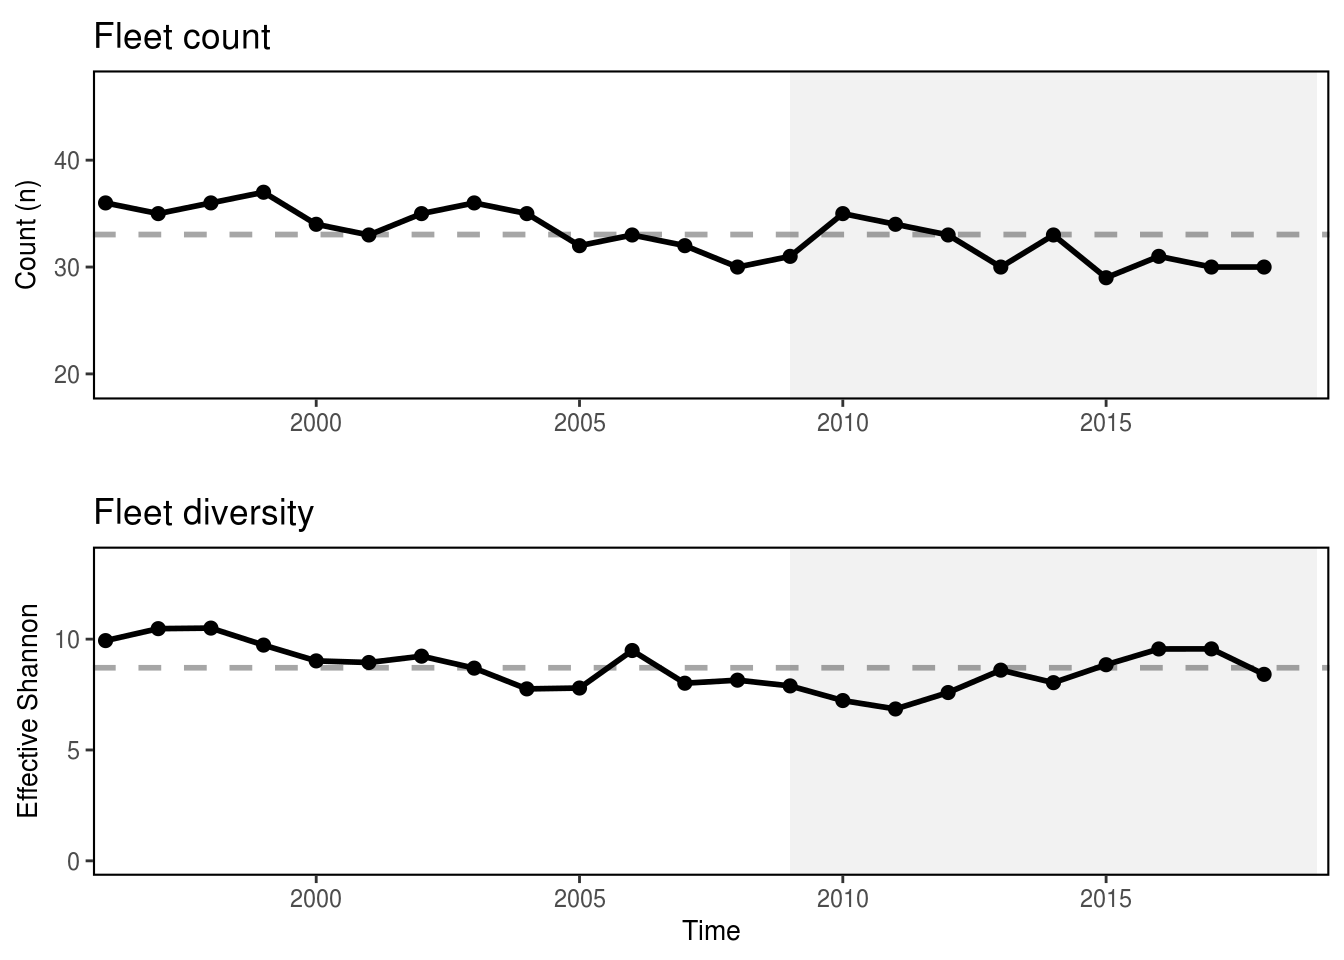
\includegraphics{/home/travis/build/NOAA-EDAB/tech-doc/images/unnamed-chunk-5-1} 

}

\caption{Fleet diversity and fleet count in the Mid-Atlantic.}\label{fig:unnamed-chunk-5}
\end{figure}

\hypertarget{chesapeake-bay-salinity}{%
\chapter{Chesapeake Bay Salinity}\label{chesapeake-bay-salinity}}

\textbf{Description}: Chesapeake Bay Salinity

\textbf{Found in}: State of the Ecosystem - Mid-Atlantic (2020)

\textbf{Indicator category}: Database pull with analysis

\textbf{Contributor(s)}: Bruce Vogt, Charles Pellerin

\textbf{Data steward}: Charles Pellerin, \href{mailto:charles.pellerin@noaa.gov}{\nolinkurl{charles.pellerin@noaa.gov}}

\textbf{Point of contact}: Bruce Vogt, \href{mailto:bruce.vogt@noaa.gov}{\nolinkurl{bruce.vogt@noaa.gov}}

\textbf{Public availability statement}: Source data are publicly available.

\hypertarget{methods-6}{%
\section{Methods}\label{methods-6}}

\hypertarget{data-sources-6}{%
\subsection{Data sources}\label{data-sources-6}}

The National Oceanic and Atmospheric Administration's (NOAA) Chesapeake Bay Interpretive Buoy System (CBIBS) is a network of observing platforms (buoys) that collect meteorological, oceanographic, and water-quality data and relay that information using wireless technology. The stations have been in place since 2007. The Sting Ray station was deployed in July of 2008 and has been monitoring conditions on and off since then. The data is recorded in situ and sent to a server over a cellular modem.

The standard CBIBS instrument is a WETLabs WQM mounted in the buoy well approximately 0.5 meters below the surface. Seabird purchased WETLabs and are now the manufacturer of the instruments. The WQM instruments are calibrated and swapped out on a regular basis. Salinity is stored as a double with the units of PSU.

\hypertarget{data-extraction-6}{%
\subsection{Data extraction}\label{data-extraction-6}}

Data is directly inserted into a database from the real time system over the cellular network. The general public can use \href{https://buoybay.noaa.gov/observations/data-download}{this link} to explore and pull that data from the CBIBS database. The process for data extraction for this indicator can be found \href{https://github.com/NOAA-EDAB/tech-doc/tree/master/R/stored_scripts/ches_bay_sal_extraction.txt}{here}.

\hypertarget{data-analysis-5}{%
\subsection{Data analysis}\label{data-analysis-5}}

The data is processed by a \href{https://github.com/NOAA-EDAB/tech-doc/tree/master/R/stored_scripts/ches_bay_sal_analysis.py}{python script}. This creates an array and runs the data through a qartod routine. The result is a set of flags. Only the good data is used in the plot below.

\hypertarget{data-processing-4}{%
\subsection{Data processing}\label{data-processing-4}}

Code for processing salinity data can be found \href{https://github.com/NOAA-EDAB/ecodata/blob/master/data-raw/get_ch_bay_sal.R}{here}.

\hypertarget{plotting-4}{%
\subsection{Plotting}\label{plotting-4}}

\begin{figure}

{\centering 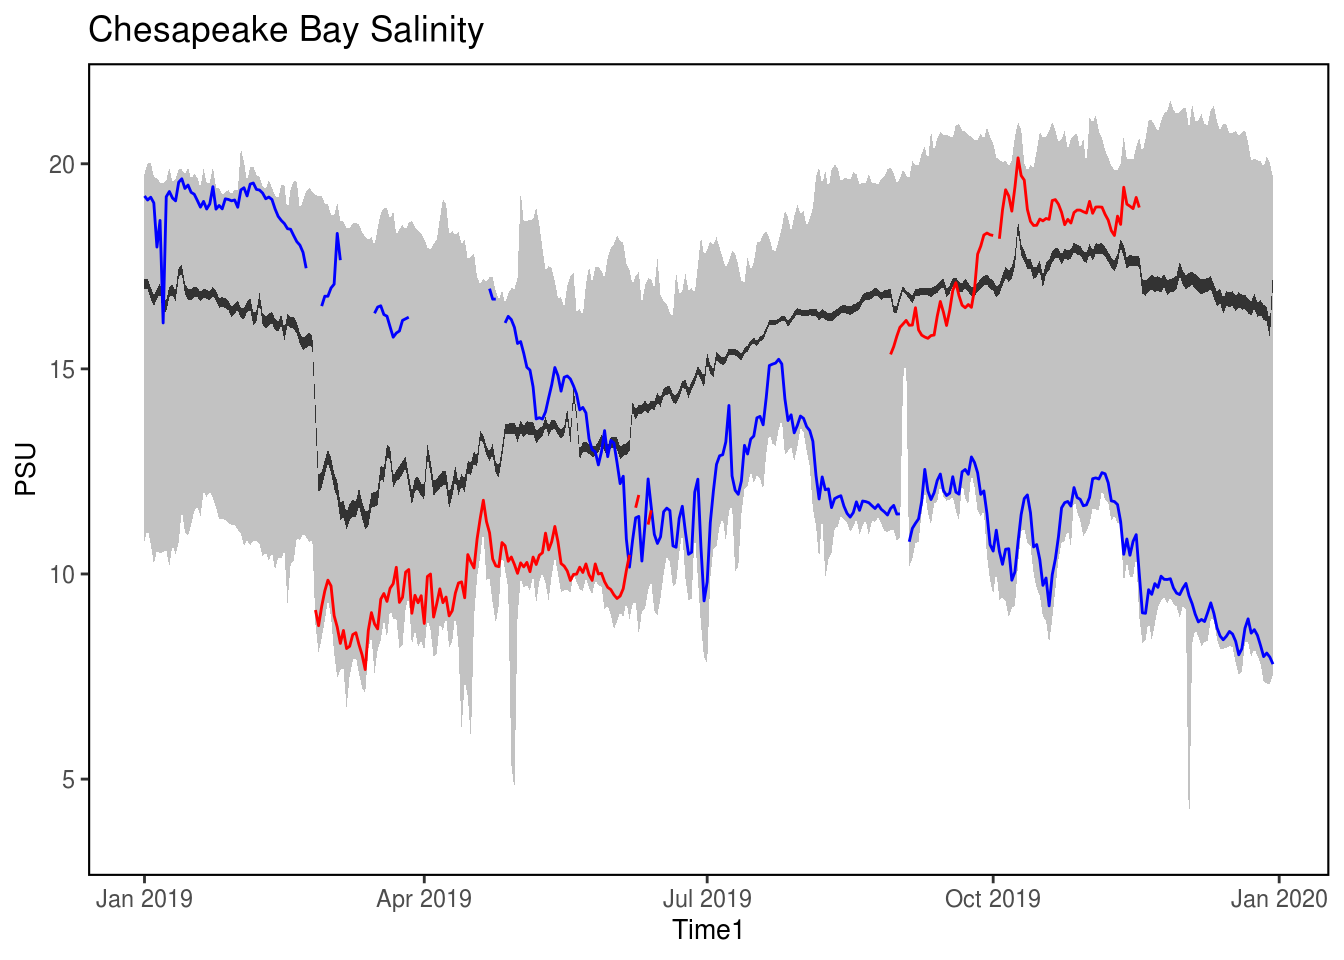
\includegraphics{/home/travis/build/NOAA-EDAB/tech-doc/images/unnamed-chunk-6-1} 

}

\caption{Buoy data showing unprecedented fresh water in Chesapeake Bay, 2018-2019.}\label{fig:unnamed-chunk-6}
\end{figure}

\hypertarget{chesapeake-bay-water-quality-standards-attainment}{%
\chapter{Chesapeake Bay Water Quality Standards Attainment}\label{chesapeake-bay-water-quality-standards-attainment}}

\textbf{Description}: A multimetric indicator describing the attainment status of Chesapeake Bay with respect to three water quality standards criteria, namely, dissolved oxygen, chlorophyll-a, and water clarity/submerged aquatic vegetation.

\textbf{Indicator category}: Published method; Database pull with analysis

\textbf{Found in}: State of the Ecosystem - Mid-Atlantic (2019)

\textbf{Contributor(s)}: Qian Zhang, Rebecca Murphy, Richard Tian, Melinda Forsyth, Emily Trentacoste, Jeni Keisman, and Peter Tango.

\textbf{Data steward}: Qian Zhang, \href{mailto:qzhang@chesapeakebay.net}{\nolinkurl{qzhang@chesapeakebay.net}}

\textbf{Point of contact}: Qian Zhang, \href{mailto:qzhang@chesapeakebay.net}{\nolinkurl{qzhang@chesapeakebay.net}}

\textbf{Public availability statement}: Data are publicly available (see Data Sources below).

\hypertarget{methods-7}{%
\section{Methods}\label{methods-7}}

To protect the aquatic living resources of Chesapeake Bay, the \href{https://www.chesapeakebay.net/}{Chesapeake Bay Program} (CBP) partnership has developed a guidance framework of ambient water quality criteria with designated uses and assessment procedures for dissolved oxygen, chlorophyll-a, and water clarity/submerged aquatic vegetation (SAV) (USEPA \protect\hyperlink{ref-usepa2003}{2003}). To achieve consistent assessment over time and between jurisdictions, a multimetric indicator was proposed by the CBP partnership to provide a means for tracking the progress in all 92 management segments of Chesapeake Bay (USEPA \protect\hyperlink{ref-usepa2017}{2017}). This indicator has been computed for each three-year assessment period since 1985-1987, providing an integrated measure of Chesapeake Bay's water quality condition over the last three decades.

\hypertarget{data-sources-7}{%
\subsection{Data sources}\label{data-sources-7}}

The multimetric indicator required monitoring data on dissolved oxygen (DO) concentrations, chlorophyll-a concentrations, water clarity, SAV acreage, water temperature, and salinity. SAV acreage has been measured by the Virginia Institute of Marine Science in collaboration with the CBP, which is available via \url{http://web.vims.edu/bio/sav/StateSegmentAreaTable.htm}. Data for all other parameters were obtained from the \href{http://www.chesapeakebay.net/data/downloads/cbp_water_quality_database_1984_present}{CBP Water Quality Database}. These data have been routinely reported to the CBP by the Maryland Department of Natural Resources, Virginia Department of Environmental Quality, Old Dominion University, Virginia Institute of Marine Science, and citizen/volunteer monitoring initiatives.

\hypertarget{data-analysis-6}{%
\subsection{Data analysis}\label{data-analysis-6}}

\textbf{Criteria attainment assessment}

Monitoring data of DO, chlorophyll-a, and water clarity/SAV were processed and compared with water quality criteria thresholds according to different designated uses (DUs). These DUs are migratory spawning and nursery (MSN), open water (OW), deep water (DW), deep channel (DC), and shallow water (SW), which reflect the seasonal nature of water column structure and the life history needs of living resources. Station-level DO and chlorophyll-a data were spatially interpolated in three dimensions.

Salinity and water temperature data were used to compute the vertical density structure of the water column, which was translated into layers of different DUs. Criteria attainment was determined by comparing violation rates over a 3-year period to a reference cumulative frequency distribution that represents the extent of allowable violation. This approach was implemented using FORTRAN codes, which are provided as a zipped folder. For water clarity/SAV, the single best year in the 3-year assessment period was compared with the segment-specific acreage goal, the water clarity goal, or a combination of both. For more details, refer to the Methods section of Zhang et al. (\protect\hyperlink{ref-zhang2018}{2018}).

\textbf{Indicator calculation}

The multimetric indicator quantifies the fraction of segment-DU-criterion combinations that meet all applicable season-specific thresholds for each 3-year assessment period from 1985-1987 to 2015-2017. For each 3-year assessment period, all applicable segment-DU-criterion combinations were evaluated in a binomial fashion and scored 1 for ``in attainment'' and 0 for ``nonattainment''. The classified status of each segment-DU-criterion combination was weighted via segments' surface area and summed to obtain the multimetric index score. This weighting scheme was adopted for two reasons: (1) segments vary in size over four orders of magnitude, and (2) surface area of each segment does not change with time or DUs, unlike seasonally variable habitat volume or bottom water area (USEPA \protect\hyperlink{ref-usepa2017}{2017}). For more details, refer to the Methods section of Zhang et al. (\protect\hyperlink{ref-zhang2018}{2018}).

The indicator provides an integrated measure of Chesapeake Bay's water quality condition (Figure 1). In 2015-2017, 42\% of all tidal water segment-DU-criterion combinations are estimated to have met or exceeded applicable water quality criteria thresholds, which marks the best 3-year status since 1985-1987. The indicator has a positive and statistically significant trend from 1985 to 2017, which shows that Chesapeake Bay is on a positive trajectory toward recovery. This pattern was statistically linked to total nitrogen reduction, indicating responsiveness of attainment status to management actions implemented to reduce nutrients in the system.

\begin{figure}
\centering
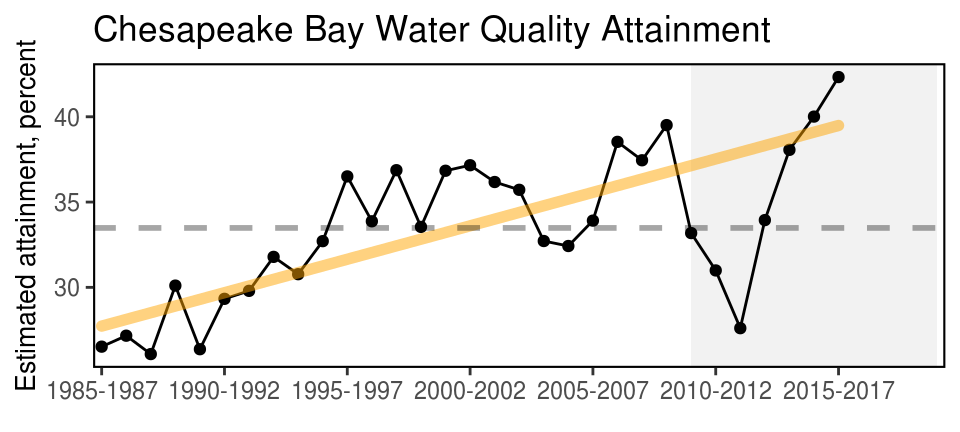
\includegraphics{/home/travis/build/NOAA-EDAB/tech-doc/images/unnamed-chunk-7-1.pdf}
\caption{\label{fig:unnamed-chunk-7}Time series of the multimetric indicator score for estimated Chesapeake Bay water quality standards attainment for each 3-year assessment period between 1985-1987 and 2015-2017. A significant positive trend for the time series is shown by the orange line (p \textless{} 0.05).}
\end{figure}

Patterns of attainment of individual DUs are variable (Figure 2). Changes in OW-DO, DC-DO, and water clarity/SAV have shown long-term improvements, which have contributed to overall attainment indicator improvement. By contrast, the MSN-DO attainment experienced a sharp spike in the first few assessment periods but generally degraded after the 1997-1999, which has implications to the survival, growth, and reproduction of the migratory and resident tidal freshwater fish during spawning and nursery season in the tidal freshwater to low-salinity habitats. The status and trends of tidal segments' attainment may be used to inform siting decisions of aquaculture operations in Chesapeake Bay.

\begin{figure}
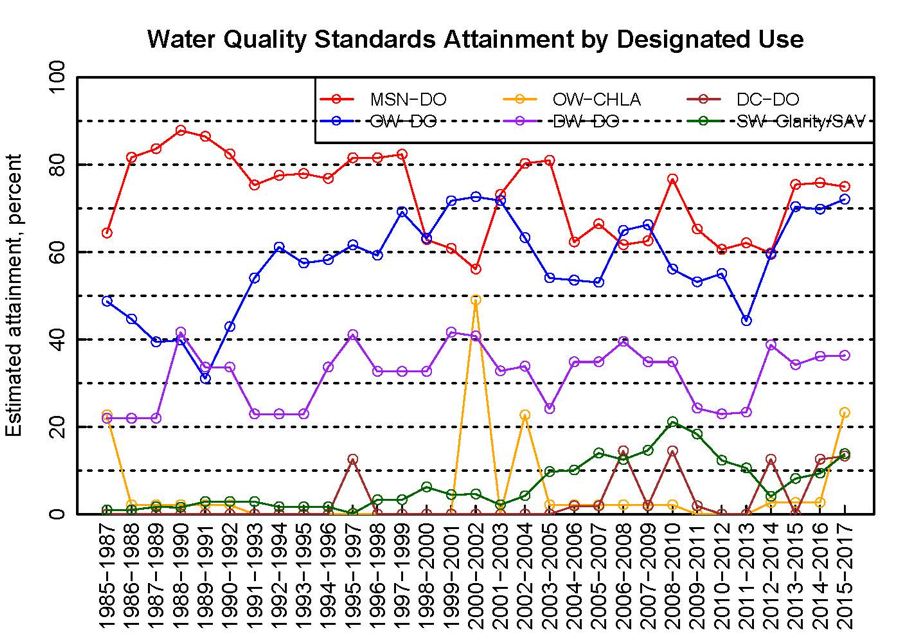
\includegraphics[width=12.49in]{/home/travis/build/NOAA-EDAB/tech-doc/images/cb_water_quality_attainment} \caption{Time series of the estimated attainment of water quality standards (i.e., DO: dissolved oxygen; CHLA: chlorophyll-a; Clarity/SAV: water clarity/submerged aquatic vegetation) for five Chesapeake Bay designated uses (MSN: migratory spawning and nursery; OW: open water; DW: deep water; DC: deep channel; SW: shallow water) for each 3-year assessment period between 1985-1987 and 2015-2017.}\label{fig:unnamed-chunk-8}
\end{figure}

\hypertarget{data-processing-5}{%
\subsection{Data processing}\label{data-processing-5}}

The indicator data set was formatted for inclusion in the ecodata R package using the R script found \href{https://github.com/NOAA-EDAB/ecodata/blob/master/data-raw/get_ches_bay_wq.R}{here}.

\hypertarget{chl-pp}{%
\chapter{\texorpdfstring{Chlorophyll \emph{a} and Primary Production}{Chlorophyll a and Primary Production}}\label{chl-pp}}

\textbf{Description}: Chlorophyll \emph{a} and Primary Production

\textbf{Found in}: State of the Ecosystem - Gulf of Maine \& Georges Bank (2018, 2019, 2020), State of the Ecosystem - Mid-Atlantic (2018, 2019, 2020)

\textbf{Indicator category}: Database pull; Database pull with analysis; Published methods

\textbf{Contributor(s)}: Kimberly Hyde

\textbf{Data steward}: Kimberly Hyde, \href{mailto:kimberly.hyde@noaa.gov}{\nolinkurl{kimberly.hyde@noaa.gov}}

\textbf{Point of contact}: Kimberly Hyde, \href{mailto:kimberly.hyde@noaa.gov}{\nolinkurl{kimberly.hyde@noaa.gov}}

\textbf{Public availability statement}: Source data used in these analyses will be made publicly available. Derived data used in State of the Ecosystem Reports can be found \href{http://comet.nefsc.noaa.gov/erddap/info/index.html?page=1\&itemsPerPage=1000}{here}.

\hypertarget{methods-8}{%
\section{Methods}\label{methods-8}}

\hypertarget{data-sources-8}{%
\subsection{Data sources}\label{data-sources-8}}

Level 1A ocean color remote sensing data from the Sea-viewing Wide Field-of-view Sensor (SeaWiFS) (NASA Ocean Biology Processing Group \protect\hyperlink{ref-NASA1}{2018}) on the OrbView-2 satellite and the Moderate Resolution Imaging Spectroradiometer (MODIS) (NASA Ocean Biology Processing Group \protect\hyperlink{ref-NASA2}{2017}) on the Aqua satellite were acquired from the NASA Ocean Biology Processing Group (OBPG). Sea Surface Temperature (SST) data included the 4 km nighttime NOAA Advanced Very High Resolution Radiometer (AVHRR) Pathfinder (Casey et al. \protect\hyperlink{ref-Casey2010}{2010}; Saha et al. \protect\hyperlink{ref-Saha2018}{2018}) and the Group for High Resolution Sea Surface Temperature (GHRSST) Multiscale Ultrahigh Resolution (MUR, version 4.1) Level 4 (Chin, Vazquez-Cuervo, and Armstrong \protect\hyperlink{ref-SOE4}{2017}; Project \protect\hyperlink{ref-SOE14}{2015}) data.

\hypertarget{data-extraction-7}{%
\subsection{Data extraction}\label{data-extraction-7}}

NA

\hypertarget{data-analysis-7}{%
\subsection{Data analysis}\label{data-analysis-7}}

The SeaWiFS and MODIS L1A files were processed using the NASA Ocean Biology Processing Group \href{https://seadas.gsfc.nasa.gov/}{SeaDAS} software version 7.4. All MODIS files were spatially subset to the U.S. East Coast (SW longitude=-82.5, SW latitude=22.5, NE longitude=-51.5, NE latitude=48.5) using \href{https://seadas.gsfc.nasa.gov/help/seadas-processing/ProcessL1aextract_modis.html}{L1AEXTRACT\_MODIS}. SeaWiFS files were subset using the same coordinates prior to begin downloaded from the \href{https://oceancolor.gsfc.nasa.gov/cgi/browse.pl?sen=am}{Ocean Color Web Browser}. SeaDAS's \href{https://seadas.gsfc.nasa.gov/help/seadas-processing/ProcessL2gen.html}{L2GEN} program was used to generate Level 2 (L2) files using the default settings and optimal ancillary files, and the \href{https://seadas.gsfc.nasa.gov/help/seadas-processing/ProcessL2bin.html}{L2BIN} program spatially and temporally aggregated the L2 files to create daily Level 3 binned (L3B) files. The daily files were binned at 2 km resolution that are stored in a global, nearly equal-area, \href{https://oceancolor.gsfc.nasa.gov/docs/format/l3bins/}{integerized sinusoidal grids} and use the default \href{https://oceancolor.gsfc.nasa.gov/atbd/ocl2flags/}{L2 ocean color flag masks}. The global SST data were also subset to the same East Coast region and remapped to the same sinusoidal grid.

The L2 files contain several ocean color products including the default chlorophyll \emph{a}; product (CHL-OCI), photosynthetic available radiation (PAR), remote sensing reflectance \((R_{rs}(\lambda))\), and several inherent optical property products (IOPs). The CHL-OCI product combines two algorithms, the O'Reilly band ratio (OCx) algorithm (O'Reilly et al. \protect\hyperlink{ref-SOE11}{1998}) and the Hu color index (CI) algorithm (Hu, Lee, and Franz \protect\hyperlink{ref-SOE5}{2012}). The SeaDAS default CHL-OCI algorithm diverges slightly from Hu, Lee, and Franz (\protect\hyperlink{ref-SOE5}{2012}) in that the transition between CI and OCx occurs at 0.15 \textless{} CI \textless{} 0.2 mg m\textsuperscript{-3} to ensure a smooth \href{https://oceancolor.gsfc.nasa.gov/atbd/chlor_a/}{transition}. The regional chlorophyll \emph{a} algorithm by Pan et al. (\protect\hyperlink{ref-SOE12}{2008}) was used to create a second chlorophyll product (CHL-PAN). CHL-PAN is an empirical algorithm derived from \emph{in situ} sampling within the Northeast Large Marine Ecosystem (NE-LME) and demonstrated significant improvements from the standard NASA operational algorithm in the NES-LME (Pan et al. \protect\hyperlink{ref-SOE13}{2010}). A 3rd-order polynomial function (Equation \eqref{eq:one}) is used to derive {[}CHL-PAN{]} from Rrs band ratios (RBR):

\begin{equation}
log[\textrm{CHL-PAN}] = A_{0} + A_{1}X + A_{2}X^{2} + A_{3}X^{3},  
\label{eq:one} 
\end{equation}

where \(X = log(R_{rs}(\lambda_{1})/R_{rs}(\lambda_{2}))\) and \(A_{i} (i = 0, 1, 2, \textrm{or } 3)\) are sensor and RBR specific coefficients:

\begin{itemize}
\tightlist
\item
  If SeaWiFS and RBR is \(R_{rs}(490)/R_{rs}(555)(R_{^3{\mskip -5mu/\mskip -3mu}_5})\) then: \(A_0=0.02534, A_1=-3.033, A_2=2.096, A_3=-1.607\)
\item
  If SeaWiFS and RBR is \(R_{rs}(490)/R_{rs}(670)(R_{^3{\mskip -5mu/\mskip -3mu}_6})\) then: \(A_0=1.351, A_1=-2.427, A_2=0.9395, A_3=-0.2432\)
\item
  If MODIS and RBR is \(R_{rs}(488)/R_{rs}(547)(R_{^3{\mskip -5mu/\mskip -3mu}_5})\) then: \(A_0=0. 03664, A_1=-3.451, A_2=2.276, A_3=-1.096\)
\item
  If MODIS and RBR is \(R_{rs}(488)/R_{rs}(667)(R_{^3{\mskip -5mu/\mskip -3mu}_6})\) then: \(A_0=1.351, A_1=-2.427, A_2=0.9395, A_3=-0.2432\)
\end{itemize}

C\textsubscript{3/5} and C\textsubscript{3/6} were calculated for each sensor specific RBR (R\textsubscript{3/5} and R\textsubscript{3/6} respectively) and then the following criteria were used to determine to derive CHL-PAN:

If \(R_{^3{\mskip -5mu/\mskip -3mu}_5}>0.15\) or \(R_{6} <0.0001\) then \(\textrm{CHL-PAN} = C_{^3{\mskip -5mu/\mskip -3mu}_5};\)

Otherwise, \(\textrm{CHL-PAN} = \textrm{max}(C_{^3{\mskip -5mu/\mskip -3mu}_5}, C_{^3{\mskip -5mu/\mskip -3mu}_6})\),

where \(R_6\) is \(R_{rs}(670)\) (SeaWiFS) or \(R_{rs}(667)\) (Pan et al. \protect\hyperlink{ref-SOE13}{2010}).

The Vertically Generalized Production Model (VGPM) estimates net primary production (PP) as a function of chlorophyll \emph{a}, photosynthetically available light and the photosynthetic efficiency (Behrenfeld and Falkowski \protect\hyperlink{ref-SOE1}{1997}). In the VGPM-Eppley version, the original temperature-dependent function to estimate the chlorophyll-specific photosynthetic efficiency is replaced with the exponential ``Eppley'' function (equation PP1) as modified by Morel (\protect\hyperlink{ref-SOE7}{1991}). The VGPM calculates the daily amount of carbon fixed based on the maximum rate of chlorophyll-specific carbon fixation in the water column, sea surface daily photosynthetically available radiation, the euphotic depth (the depth where light is 1\% of that at the surface), chlorophyll \emph{a} concentration, and the number of daylight hours (Equation \eqref{eq:two}).

\begin{equation}
P_{max}^{b}(SST) = 4.6 * 1.065^{SST-20^{0}} 
\label{eq:two} 
\end{equation}
Where \(P_{max}^{b}\) is the maximum carbon fixation rate and \emph{SST} is sea surface temperature.

\begin{equation}
PP_{eu} = 0.66125 * P_{max}^{b} * \frac{I_{0}}{I_{0}+4.1} * Z_{eu} * \textrm{CHL} * \text{DL}
\label{eq:three} 
\end{equation}

Where \(PP_{eu}\) is the daily amount of carbon fixed integrated from the surface to the euphotic depth (mgC m\textsuperscript{-2} day\textsuperscript{-1}), \(P_{max}^{b}\) is the maximum carbon fixation rate within the water column (mgC mgChl\textsuperscript{-1} hr\textsuperscript{-1}), \(I_{0}\) is the daily integrated molar photon flux of sea surface PAR (mol quanta m\textsuperscript{-2} day\textsuperscript{-1}), Zeu is the euphotic depth (m), CHL is the daily interpolated CHIi-OCI (mg m\textsuperscript{-3}), and DL is the photoperiod (hours) calculated for the day of the year and latitude according to Kirk (\protect\hyperlink{ref-SOE6}{1994}). The light dependent function \((I_{0}/(I_{0}+4.1))\) describes the relative change in the light saturation fraction of the euphotic zone as a function of surface PAR (\(I_0\)). Zeu is derived from an estimate of the total chlorophyll concentration within the euphotic layer (\emph{CHL\textsubscript{eu}}) based on the Case I models of Morel and Berthon (\protect\hyperlink{ref-SOE8}{1989}):

\begin{itemize}
\tightlist
\item
  For \(\textrm{CHL}_{eu} > 10.0\;\;\;\;\;Z_{eu} = 568.2 * \textrm{CHL}_{eu}^{-0.746}\)
\item
  For \(\textrm{CHL}_{eu} \leq 10.0\;\;\;\;\;Z_{eu} = 200.0 * \textrm{CHL}_{eu}^{-0.293}\)
\item
  For \(\textrm{CHL}_{0} \leq 1.0\;\;\;\;\;\textrm{CHL}_{eu} = 38.0 * \textrm{CHL}_{0}^{0.425}\)
\item
  For \(\textrm{CHL}_{0} > 1.0\;\;\;\;\;\textrm{CHL}_{eu} = 40.2 * \textrm{CHL}_{0}^{0.507}\)
\end{itemize}

Where \(\textrm{CHL}_0\) is the surface chlorophyll concentration.

Prior to being input into the VGPM-Eppley model, the daily CHL-OCI and AVHRR SST data were temporally interpolated and smoothed (CHL-OCI\textsubscript{INT} and SST\textsubscript{INT} respectively) to increase the data coverage and better match data collected from different sensors and different times. The daily PAR data are not affected by cloud cover and MUR SST data is a blended/gap free data product so these products were not interpolated.

Daily data at each pixel location covering the entire date range were extracted to create a pixel time series \((D_{x,y})\). \((D_{x,y})\) are linearly interpolated based on days in the time series using \href{https://github.com/callumenator/idl/blob/master/external/JHUAPL/INTERPX.PRO}{interpx.pro}. Prior to interpolation, the CHL data are log-transformed to account for the log-normal distribution of chlorophyll data (Campbell \protect\hyperlink{ref-SOE2}{1995}). Interpolating the entire times series requires a large amount of processing time so the series was processed one year at a time. Each yearly series included 60 days from the previous year and 60 days from the following year to improve the interpolation at the beginning and end of the year. Following interpolation, the data are smoothed with a tri-cube filter (width=7) using IDL's \href{https://www.harrisgeospatial.com/docs/CONVOL.html}{CONVOL} program. In order to avoid over interpolating data when there were several days of missing data in the time series, the interpolated data were removed and replaced with blank data if the window of interpolation spanned more than 7 days for CHL or 10 days for SST. After all D\textsubscript{x,y} pixels had been processed, the one-dimensional pixel time series were converted back to two-dimensional daily files.

Statistics, including the arithmetic mean, geometric mean (for CHL and PP), standard deviation, and coefficient of variation were calculated at daily (3 and 8-day running means), weekly, monthly, and annual time steps and for several climatological periods. Annual statistics used the monthly means as inputs to avoid a summer time bias when more data is available due to reduced cloud cover. The daily, weekly, monthly and annual climatological statistics include the entire time series for each specified period. For example, the climatological January uses the monthly mean from each January in the time series and the climatological annual uses the annual mean from each year. The CHL and PP climatological statistics include data from both SeaWiFS (1997-2007) and MODIS (2008-2017).

Weekly, monthly and annual anomalies were calculated for each product by taking the difference between the mean of the input time period (i.e.~week, month, year) and the climatological mean for the same period. Because bio-optical data are typically log-normally distributed (Campbell \protect\hyperlink{ref-SOE2}{1995}), the CHL and PP data were first log-transformed prior to taking the difference and then untransformed, resulting in an anomaly ratio.

The ecological production unit (EPU) shapefile that excludes the estuaries was used to spatially extract all data location within an ecoregion from the statistic and anomaly files. The median values, which are equivalent to the geometric mean, were used for the CHL and PP data. For the extended time series, the 1998-2007 data use the SeaWiFS ocean color products and MODIS-Aqua products were used from 2008 to 2017. Prior to June 2002, AVHRR Pathfinder data are used as the SST source and MUR SST in subsequent years.

\hypertarget{data-processing-6}{%
\subsection{Data processing}\label{data-processing-6}}

CHL and PPD time series were formatted for inclusion in the \texttt{ecodata} R package using the R code found \href{https://github.com/NOAA-EDAB/ecodata/blob/master/data-raw/get_chl_pp.R}{here}.

\hypertarget{plotting-5}{%
\subsection{Plotting}\label{plotting-5}}

Chl \emph{a} and primary production data were also examined in relation to the long-term means of each series. The figures below show data specific to the Mid-Atlantic Bight. The code for the plots can be found \href{https://github.com/NOAA-EDAB/ecodata/blob/master/chunk-scripts/LTL.Rmd-mab-chl-weekly.R}{here}.

\begin{figure}
\centering
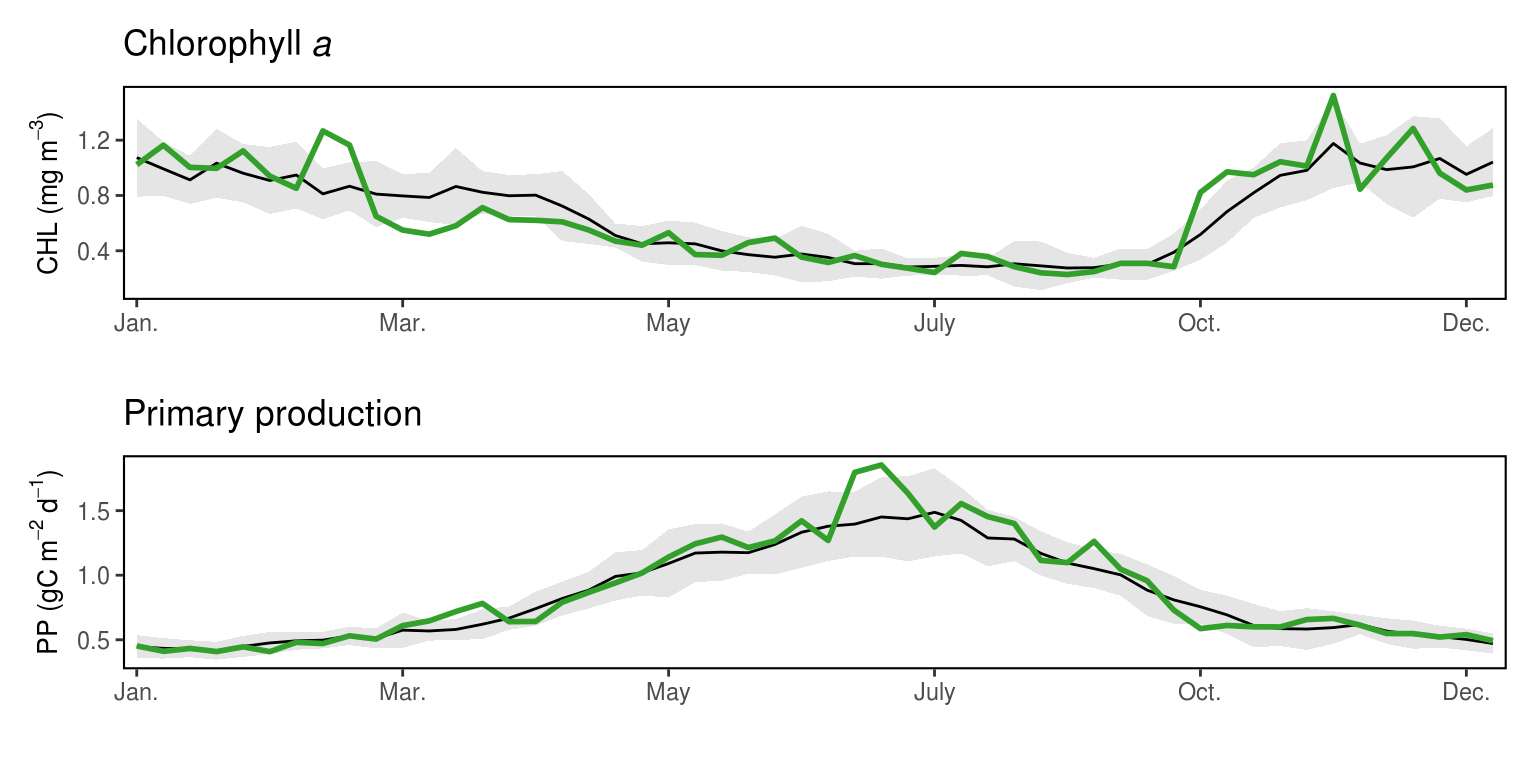
\includegraphics{/home/travis/build/NOAA-EDAB/tech-doc/images/unnamed-chunk-9-1.pdf}
\caption{\label{fig:unnamed-chunk-9}Weekly chlorophyll concentrations in the Mid-Atlantic are shown by the colored line for 2019. The long-term mean is shown in black, and shading indicates +/- 1 sample SD.}
\end{figure}

In the figure below, we show monthly primary productivity on an annual time step in the Mid-Atlantic Bight. The code for this can be found \href{https://github.com/NOAA-EDAB/ecodata/blob/master/chunk-scripts/LTL.Rmd-PP-OCCI.R}{here}

\begin{figure}
\centering
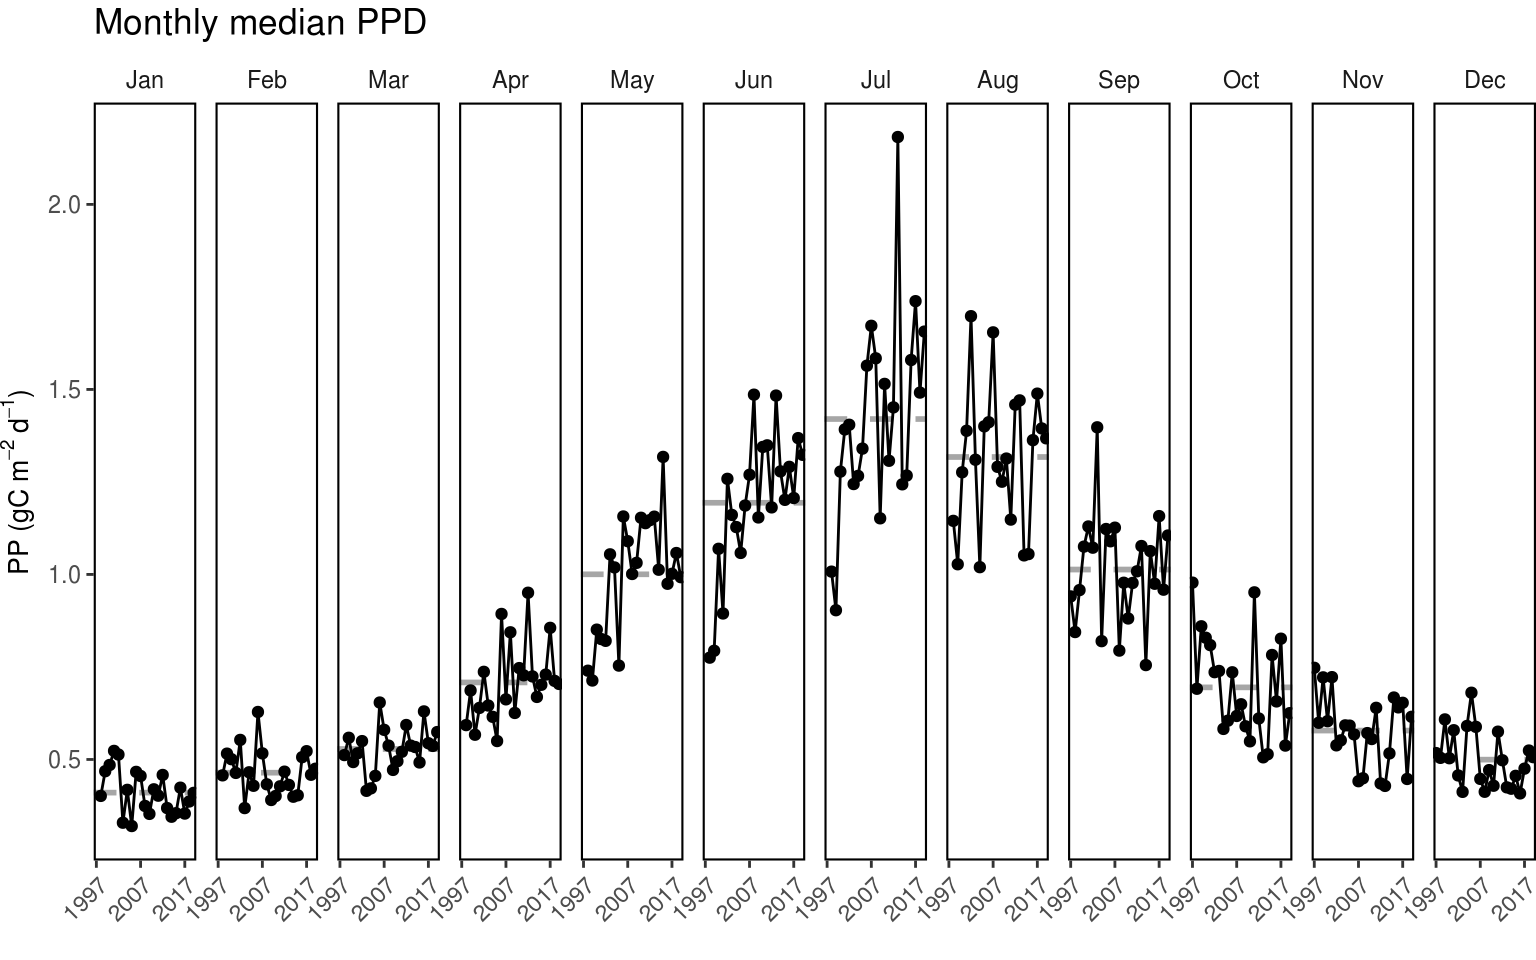
\includegraphics{/home/travis/build/NOAA-EDAB/tech-doc/images/unnamed-chunk-10-1.pdf}
\caption{\label{fig:unnamed-chunk-10}Monthly primary production trends show the annual cycle (i.e.~the peak during the summer months) and the changes over time for each month.}
\end{figure}

\hypertarget{cold-pool-index}{%
\chapter{Cold Pool Index}\label{cold-pool-index}}

\textbf{Description}: Cold Pool Index

\textbf{Found in}: State of the Ecosystem - Mid-Atlantic (2020)

\textbf{Indicator category}: Published methods

\textbf{Contributor(s)}: Chris Melrose

\textbf{Data steward}: Kimberly Bastille

\textbf{Point of contact}: Chris Melrose \href{mailto:chris.melrose@noaa.gov}{\nolinkurl{chris.melrose@noaa.gov}}

\textbf{Public availability statement}: Source data are publicly available.

\hypertarget{methods-9}{%
\section{Methods}\label{methods-9}}

\hypertarget{data-sources-9}{%
\subsection{Data sources}\label{data-sources-9}}

NEFSC Hydrographic Database
This data represents the annual mean bottom temperature residual for Sept-Oct in the Mid-Atlantic Bight cold pool region from 1977-2018.

\hypertarget{data-extraction-8}{%
\subsection{Data extraction}\label{data-extraction-8}}

\hypertarget{data-analysis-8}{%
\subsection{Data analysis}\label{data-analysis-8}}

Methods published T. Miller, Hare, and Alade (\protect\hyperlink{ref-miller2016}{2016}), \href{https://github.com/NOAA-EDAB/tech-doc/tree/master/R/stored_scripts/cold_pool_analysis.txt}{original MATLAB source code} used in that paper was provided by Jon Hare and used in this analysis.

\hypertarget{data-processing-7}{%
\subsection{Data processing}\label{data-processing-7}}

Code used to process the cold pool inidcator can be found in the \texttt{ecodata} package \href{https://github.com/NOAA-EDAB/ecodata/blob/master/data-raw/get_cold_pool.R}{here}.

\hypertarget{plotting-6}{%
\subsection{Plotting}\label{plotting-6}}

The plot below was built using the code found
\href{https://github.com/NOAA-EDAB/ecodata/blob/master/chunk-scripts/LTL.Rmd-cold_pool.R}{here}.

\begin{figure}

{\centering 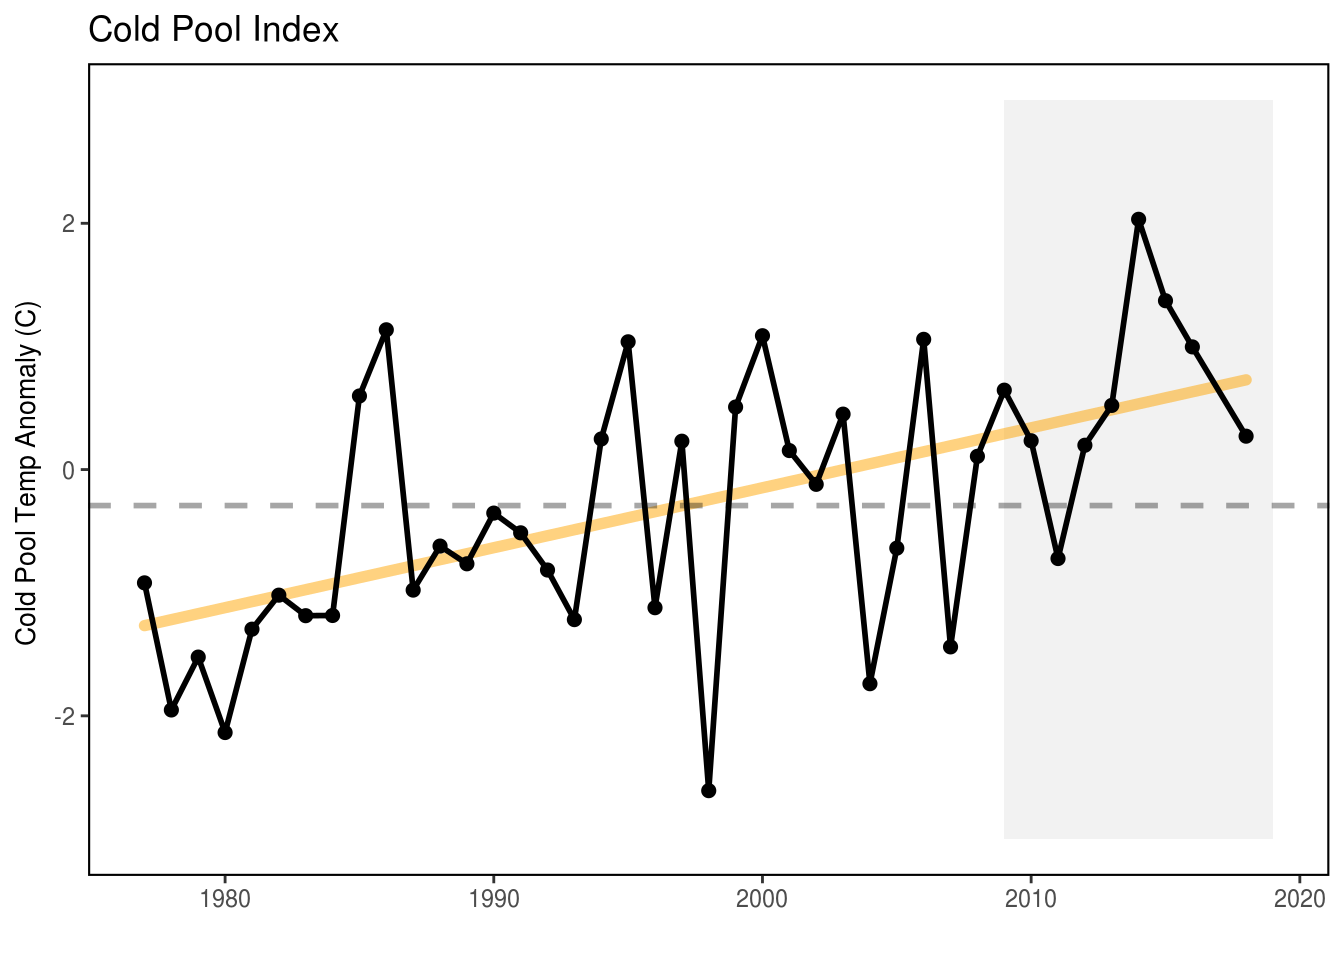
\includegraphics{/home/travis/build/NOAA-EDAB/tech-doc/images/unnamed-chunk-11-1} 

}

\caption{Cold Pool Index}\label{fig:unnamed-chunk-11}
\end{figure}

\hypertarget{comdat}{%
\chapter{Commercial Landings Data}\label{comdat}}

\textbf{Description}: Commercial landings data pull

\textbf{Found in}: State of the Ecosystem - Gulf of Maine \& Georges Bank (2017, 2018, 2019,2020), State of the Ecosystem - Mid-Atlantic (2017, 2018, 2019,2020)

\textbf{Indicator category}: Database pull

\textbf{Contributor(s)}: Sean Lucey

\textbf{Data steward}: Sean Lucey, \href{mailto:Sean.Lucey@noaa.gov}{\nolinkurl{Sean.Lucey@noaa.gov}}

\textbf{Point of contact}: Sean Lucey, \href{mailto:Sean.Lucey@noaa.gov}{\nolinkurl{Sean.Lucey@noaa.gov}}

\textbf{Public availability statement}: Raw data are not publically available due to confidentiality of individual fishery participants. Derived indicator outputs are
available \href{https://comet.nefsc.noaa.gov/erddap/tabledap/group_landings_soe_v1.html}{here}.

\hypertarget{methods-10}{%
\section{Methods}\label{methods-10}}

Fisheries dependent data for the Northeast Shelf extend back several decades. Data from the 1960s on are housed in the Commercial database (CFDBS) of the Northeast Fisheries Science Center which contains the commercial fisheries dealer purchase records (weigh-outs) collected by National Marine Fisheries Service (NMFS) Statistical Reporting Specialists and state agencies from Maine to Virginia. The data format has changed slightly over the time series with three distinct time frames as noted in Table \ref{tab:calibration1} below.

\begin{table}

\caption{\label{tab:calibration1}Data formats}
\centering
\begin{tabular}[t]{ll}
\toprule
Table & Years\\
\midrule
WOLANDS & 1964 - 1981\\
WODETS & 1982 - 1993\\
CFDETS\_AA & > 1994\\
\bottomrule
\end{tabular}
\end{table}

Comlands is an R database pull that consolidates the landings records from 1964 on and attempts to associate them with NAFO statistical areas (Figure \ref{fig:StatAreaMap}). The script is divided into three sections. The first pulls domestic landings data from the yearly landings tables and merges them into a single data source. The second section applies an algorithm to associate landings that are not allocated to a statistical area using similar characteristics of the trip to trips with known areas. The final section pulls foreign landings from the Northwest Atlantic Fisheries Organization website and rectifies species and gear codes so they can be merged along with domestic landings.

\begin{figure}

{\centering 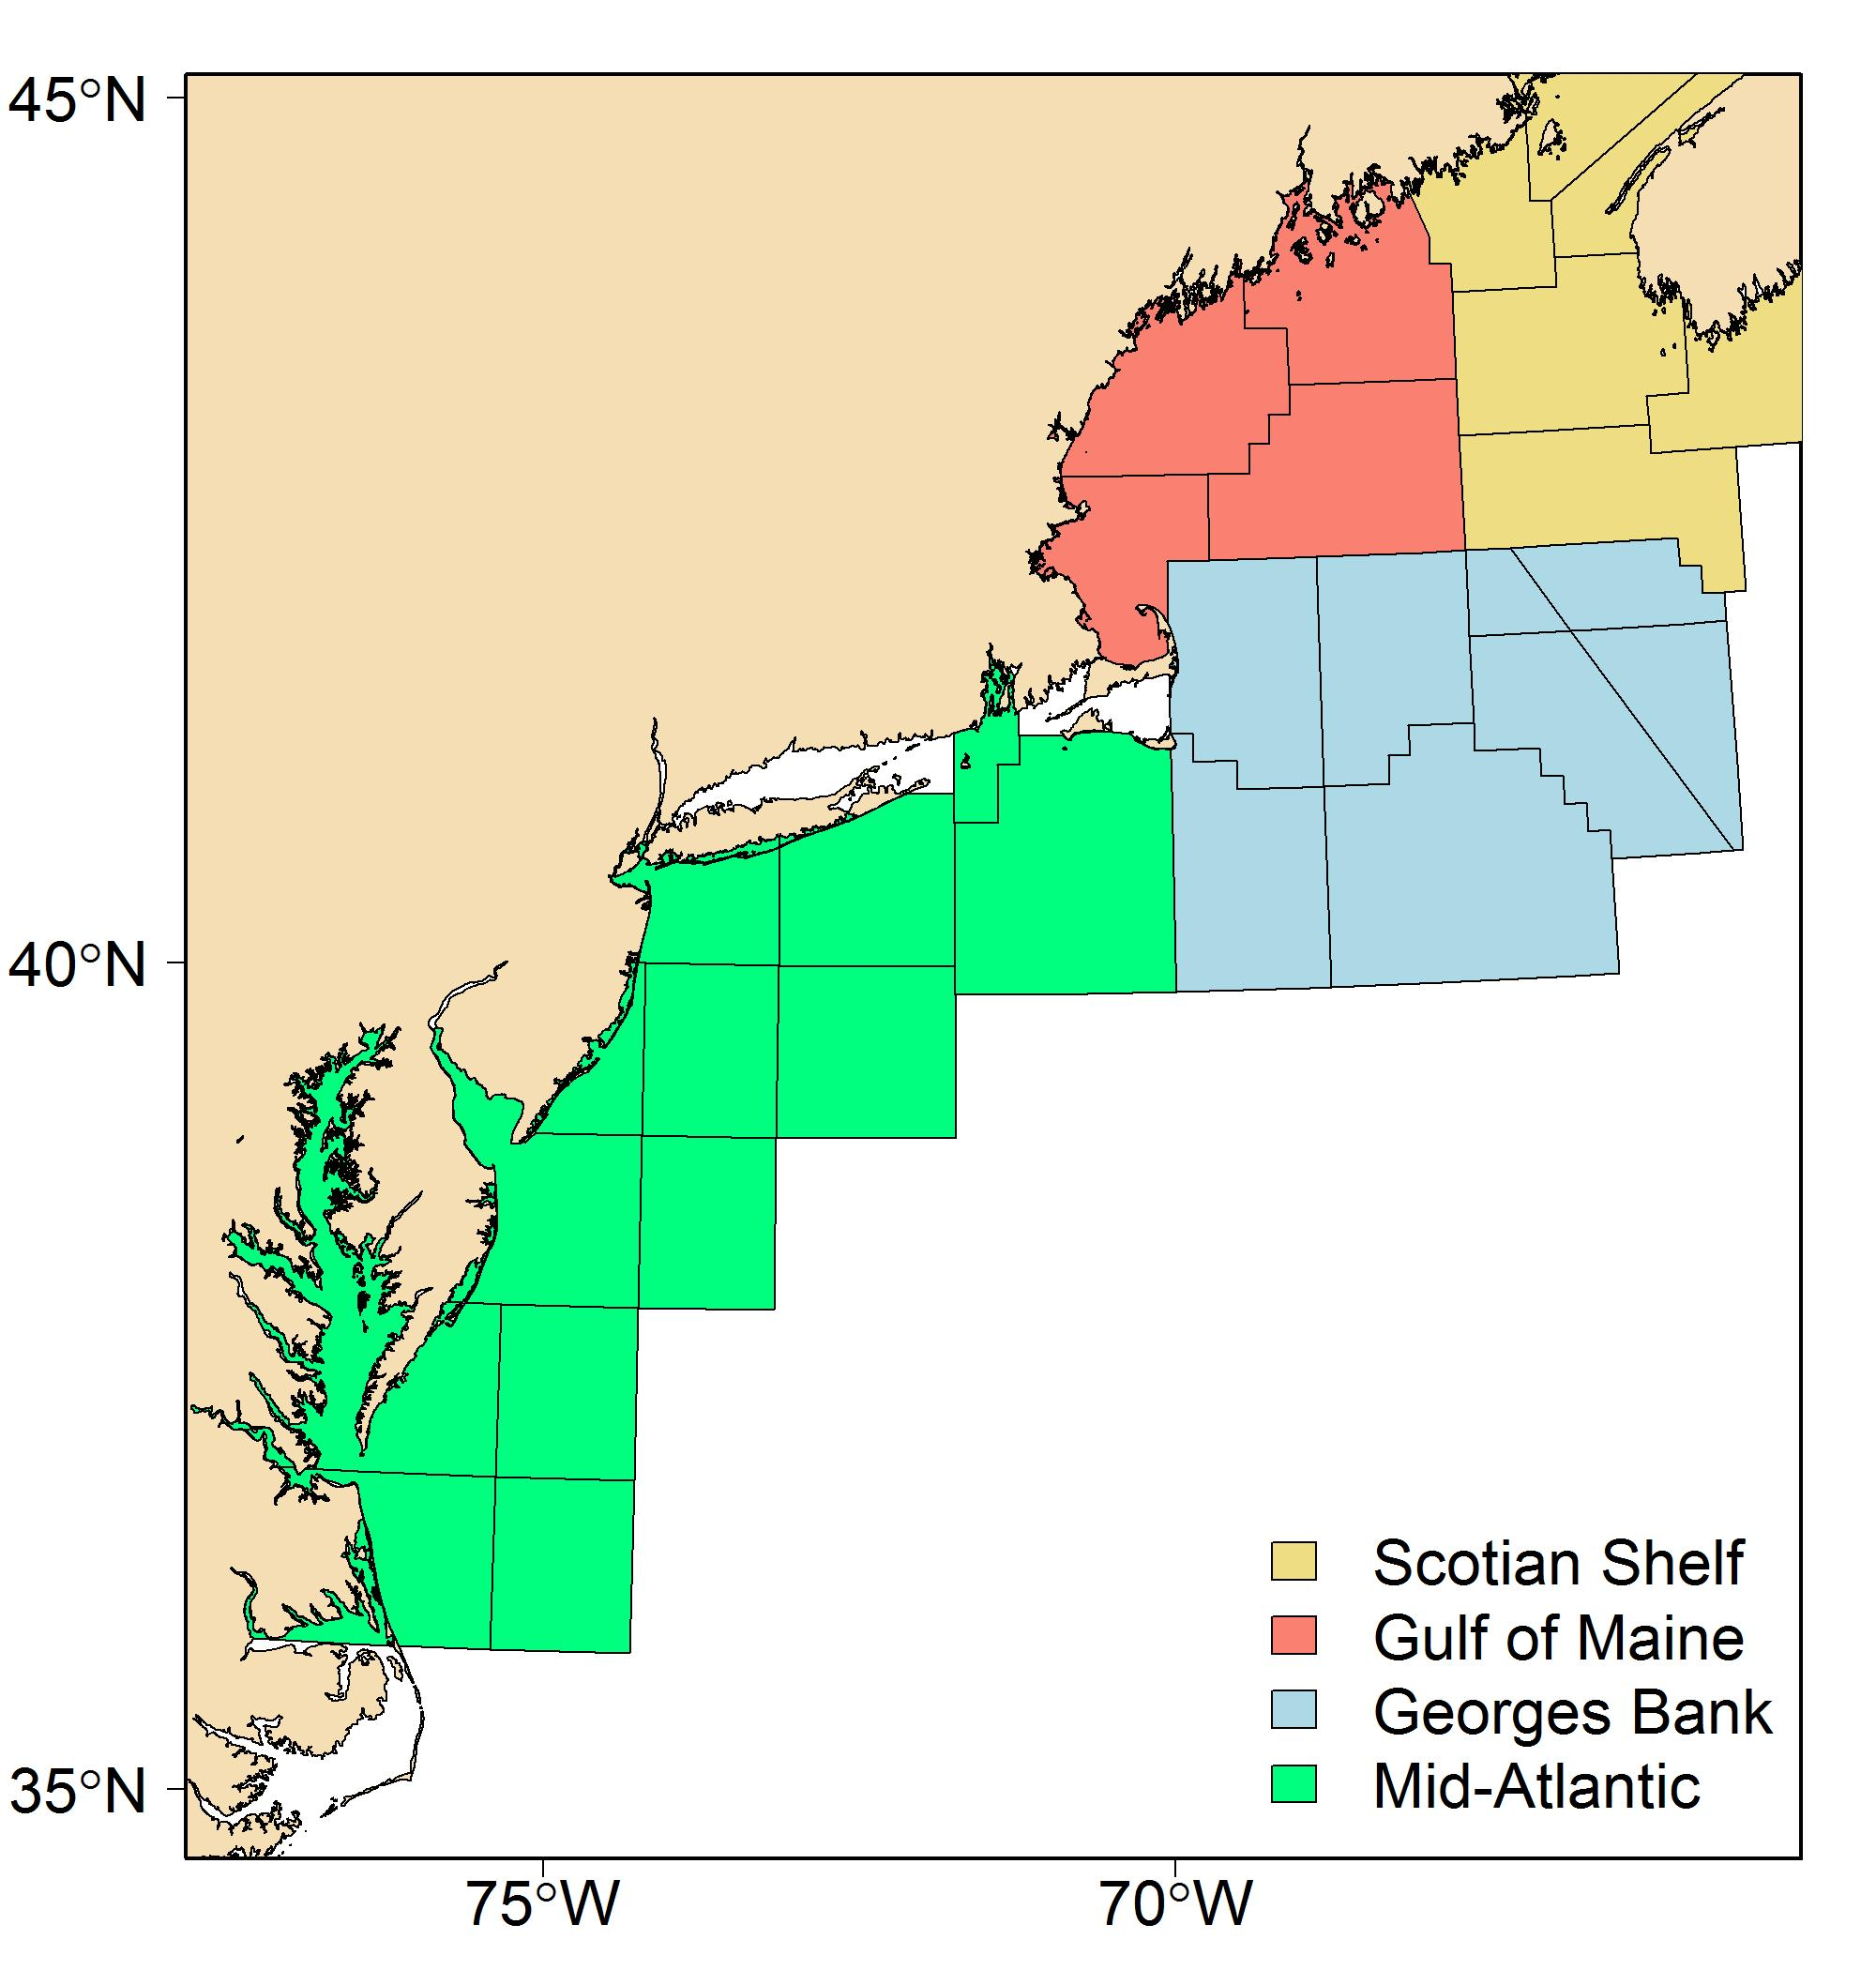
\includegraphics[width=0.5\linewidth]{/home/travis/build/NOAA-EDAB/tech-doc/images/Stat_Area_Map} 

}

\caption{Map of the North Atlantic Fisheries Organization (NAFO) Statistical Areas.  Colors represent the Ecological Production Unit (EPU) with which the statistical area is associated.}\label{fig:StatAreaMap}
\end{figure}

During the first section, the Comlands script pulls the temporal and spatial information as well as vessel and gear characteristics associated with the landings in addition to the weight, value, and utilization code of each species in the landings record. The script includes a toggle to use landed weights as opposed to live weights. For all but shellfish species, live weights are used for the State of the Ecosystem report. Due to the volume of data contained within each yearly landings table, landings are aggregated by species, utilization code, and area as well as by month, gear, and tonnage class. All weights are then converted from pounds to metric tons. Landings values are also adjusted for inflation using the Producer Price Index by Commodity for Processed Foods and Feeds: Unprocessed and Packaged Fish. Inflation is based on January of the terminal year of the data pull ensuring that all values are in current dollar prices.

\begin{table}

\caption{\label{tab:geartypes}Gear types used in commercial landings}
\centering
\begin{tabular}[t]{rl}
\toprule
 & Major gear\\
\midrule
1 & Otter Trawls\\
2 & Scallop Dredges\\
3 & Other Dredges\\
4 & Gillnets\\
5 & Longlines\\
\addlinespace
6 & Seines\\
7 & Pots/Traps\\
8 & Midwater\\
9 & Other\\
\bottomrule
\end{tabular}
\end{table}

Several species have additional steps after the data is pulled from CFDBS. Skates are typically landed as a species complex. In order to segregate the catch into species, the ratio of individual skate species in the NEFSC bottom trawl survey is used to disaggregate the landings. A similar algorithm is used to separate silver and offshore hake which can be mistaken for one another. Finally, Atlantic herring landings are pulled from a separate database as the most accurate weights are housed by the State of Maine. Comlands pulls from the State database and replaces the less accurate numbers from the federal database.

The majority of landings data are associated with a NAFO Statistical Area. For those that are not, Comlands attempts to assign them to an area using similar characteristics of trips where the area is known. To simplify this task, landings data are further aggregated into quarter and half year, small and large vessels, and eight major gear categories (Table \ref{tab:geartypes}). Landings are then proportioned to areas that meet similar characteristics based on the proportion of landings in each area by that temporal/vessel/gear combination. If a given attribute is unknown, the algorithm attempts to assign it one, once again based on matched characteristics of known trips. Statistical areas are then assigned to their respective \protect\hyperlink{epu}{Ecological Production Unit} (Table \ref{tab:statareas}).

\begin{table}[H]

\caption{\label{tab:statareas}Statistical areas making up each EPU}
\centering
\begin{tabular}[t]{l|l}
\hline
EPU & Stat Areas\\
\hline
Gulf of Maine & 500, 510, 512, 513, 514, 515\\
\hline
Georges Bank & 521, 522, 523, 524, 525, 526, 551, 552, 561, 562\\
\hline
Mid-Atlantic & 537, 539, 600, 612, 613, 614, 615, 616, 621, 622, 625, 626, 631, 632\\
\hline
\end{tabular}
\end{table}

The final step of Comlands is to pull the foreign landings from the \href{https://www.nafo.int/Data/frames}{NAFO database}. US landings are removed from this extraction so as not to be double counted. NAFO codes and CFDBS codes differ so the script rectifies those codes to ensure that the data is seamlessly merged into the domestic landings. Foreign landings are flagged so that they can be removed if so desired.

\hypertarget{data-sources-10}{%
\subsection{Data sources}\label{data-sources-10}}

Comland is a database query of the NEFSC commercial fishery database (CFDBS). More information about the CFDBS is available \href{https://inport.nmfs.noaa.gov/inport/item/27401}{here}.

\hypertarget{data-extraction-9}{%
\subsection{Data extraction}\label{data-extraction-9}}

\href{https://github.com/NOAA-EDAB/comlandr}{\texttt{comlandr}} is a package used to extract relevant data from the database.

\hypertarget{data-processing-8}{%
\subsubsection{Data Processing}\label{data-processing-8}}

The landings data were formatted for inclusion in the \texttt{ecodata} R package with this \href{https://github.com/NOAA-EDAB/ecodata/blob/master/data-raw/get_comdat.R}{R code}.

\hypertarget{data-analysis-9}{%
\subsection{Data analysis}\label{data-analysis-9}}

Fisheries dependent data from Comlands is used in several indicators for the State of the Ecosystem report; the more complicated analyses are detailed in their own sections. The most straightforward use of this data are the aggregate landings indicators. These are calculated by first assigning the various species into \protect\hyperlink{aggroups}{aggregate groups}. Species are also marked by which management body manages them. Landings are then summed by year, \protect\hyperlink{epu}{EPU}, aggregate group, and whether they are managed or not. Both managed and unmanaged totals are added together to get the final amount of total landings for that aggregate group within its respective region. Both the total and those landings managed by the management body receiving the report are reported. Proportions of managed landings to total landings are also reported in tabular form.

\hypertarget{plotting-7}{%
\subsection{Plotting}\label{plotting-7}}

The plot below was built using the code found
\href{https://github.com/NOAA-EDAB/ecodata/blob/master/chunk-scripts/human_dimensions.Rmd-comm_landings.R}{here}.

\begin{figure}

{\centering 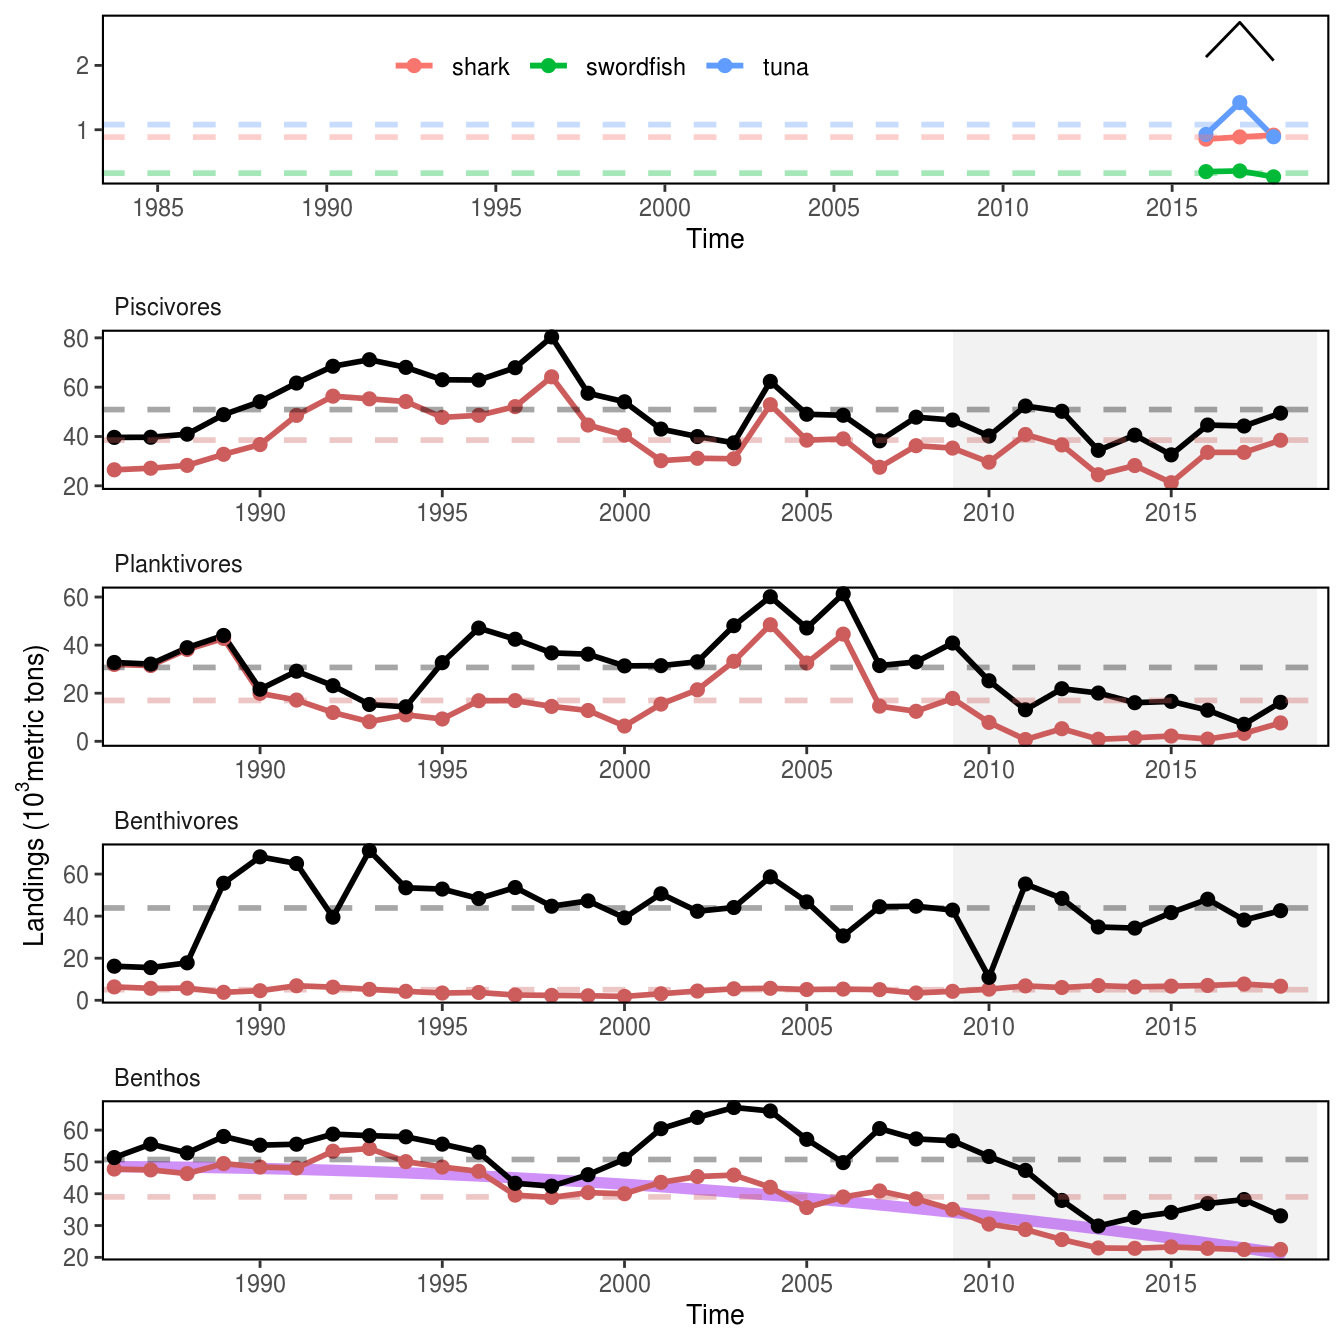
\includegraphics{/home/travis/build/NOAA-EDAB/tech-doc/images/unnamed-chunk-12-1} 

}

\caption{Mid-Atlantic commercial landings.}\label{fig:unnamed-chunk-12}
\end{figure}

\hypertarget{community-engagement}{%
\chapter{Community Engagement}\label{community-engagement}}

\textbf{Description}: Fishing community engagement

\textbf{Found in}: State of the Ecosystem - Gulf of Maine \& Georges Bank (2020), State of the Ecosystem - Mid-Atlantic (2020)

\textbf{Indicator category}: Database pull with analysis

\textbf{Contributor(s)}: Lisa L. Colburn

\textbf{Data steward}: Lisa L. Colburn

\textbf{Point of contact}: Lisa L. Colburn

\textbf{Public availability statement}: The source data used to construct the commercial fishing engagement and reliance indices include confidential information and are not available publicly. However, the commercial fishing engagement and reliance indices are not confidential so are available to the public. All calculated indices can be found \href{https://www.fisheries.noaa.gov/national/socioeconomics/social-indicators-fishing-communities-0}{here}.

\hypertarget{methods-11}{%
\section{Methods}\label{methods-11}}

\hypertarget{data-sources-11}{%
\subsection{Data sources}\label{data-sources-11}}

NOAA Fisheries' Community Social Vulnerability Indicators (CSVIs) were developed using secondary data including social, demographic and fisheries variables. The social and demographic data were downloaded from the 2014 American Community Survey (ACS) 5-yr estimates Dataset at the \href{https://www.census.gov/programs-surveys/acs/}{U.S. Census American Community Survey (ACS) site} for coastal communities at the Census Designated Place (CDP) level, and in some cases the County Subdivision (MCD) level. Commercial fisheries data were pulled from the SOLE server located at Northeast Fisheries Science Center in Woods Hole, MA. The recreational fishing information is publicly accessible through the \href{https://www.st.nmfs.noaa.gov/recreational-fisheries/MRIP/}{Marine Recreational Information Program (MRIP)}, and for this analysis was custom requested from NOAA Fisheries headquarters.

\hypertarget{data-extraction-10}{%
\subsection{Data extraction}\label{data-extraction-10}}

Commercial fisheries data was pulled from the NEFSC SOLE server in Woods Hole, MA.

SQL and SAS code for data extraction and processing steps can be found \href{https://github.com/NOAA-EDAB/tech-doc/tree/master/R/stored_scripts/comm_rel_vuln_extraction.sql}{here}.

\hypertarget{data-analysis-10}{%
\subsection{Data analysis}\label{data-analysis-10}}

The indicators were developed using the methodology described in Jacob et al. (\protect\hyperlink{ref-Jacob2010}{2010}), Jacob et al. (\protect\hyperlink{ref-Jacob2013}{2013}), L. L. Colburn and Jepson (\protect\hyperlink{ref-colburn2012}{2012}\protect\hyperlink{ref-colburn2012}{a}) and M. Jepson and Colburn (\protect\hyperlink{ref-Jepson2013}{2013}). Indicators were constructed through principal component analysis with a single factor solution, and the following criteria had to have been met: a minimum variance explained of 45\%; Kasier-Meyer Olkin measure of sampling adequacy above.500; factor loadings above.350; Bartlett's test of sphericity significance above .05; and an Armor's Theta reliability coefficient above .500. Factor scores for each community were ranked based on standard deviations into the following categories: High(\textgreater=1.00SD), MedHigh .500-.999 SD), Moderate (.000-.499 SD) and Low (\textless.000 SD).

\hypertarget{data-processing-9}{%
\subsection{Data processing}\label{data-processing-9}}

Data were formatted for inclusion in the ecodata R package using the R script found \href{https://raw.githubusercontent.com/NOAA-EDAB/ecodata/master/data-raw/get_engagement.R}{here}.

\hypertarget{plotting-8}{%
\subsection{Plotting}\label{plotting-8}}

Code used to build the community engagement indicator plot below can be found \href{https://github.com/NOAA-EDAB/ecodata/blob/master/chunk-scripts/LTL.Rmd-MAB-comm-eng.R}{here}.

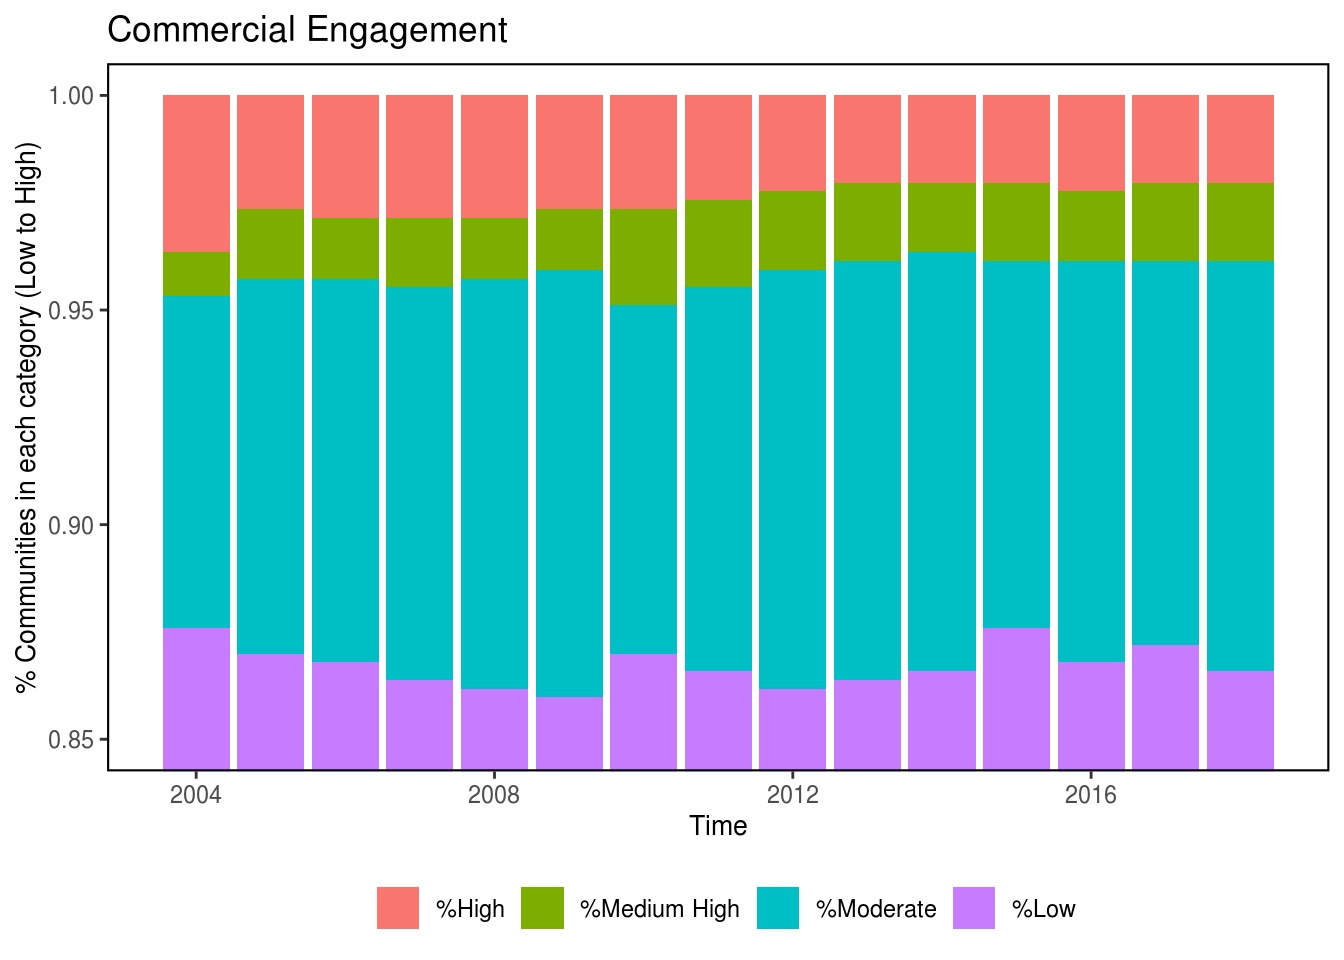
\includegraphics{/home/travis/build/NOAA-EDAB/tech-doc/images/unnamed-chunk-13-1.pdf} 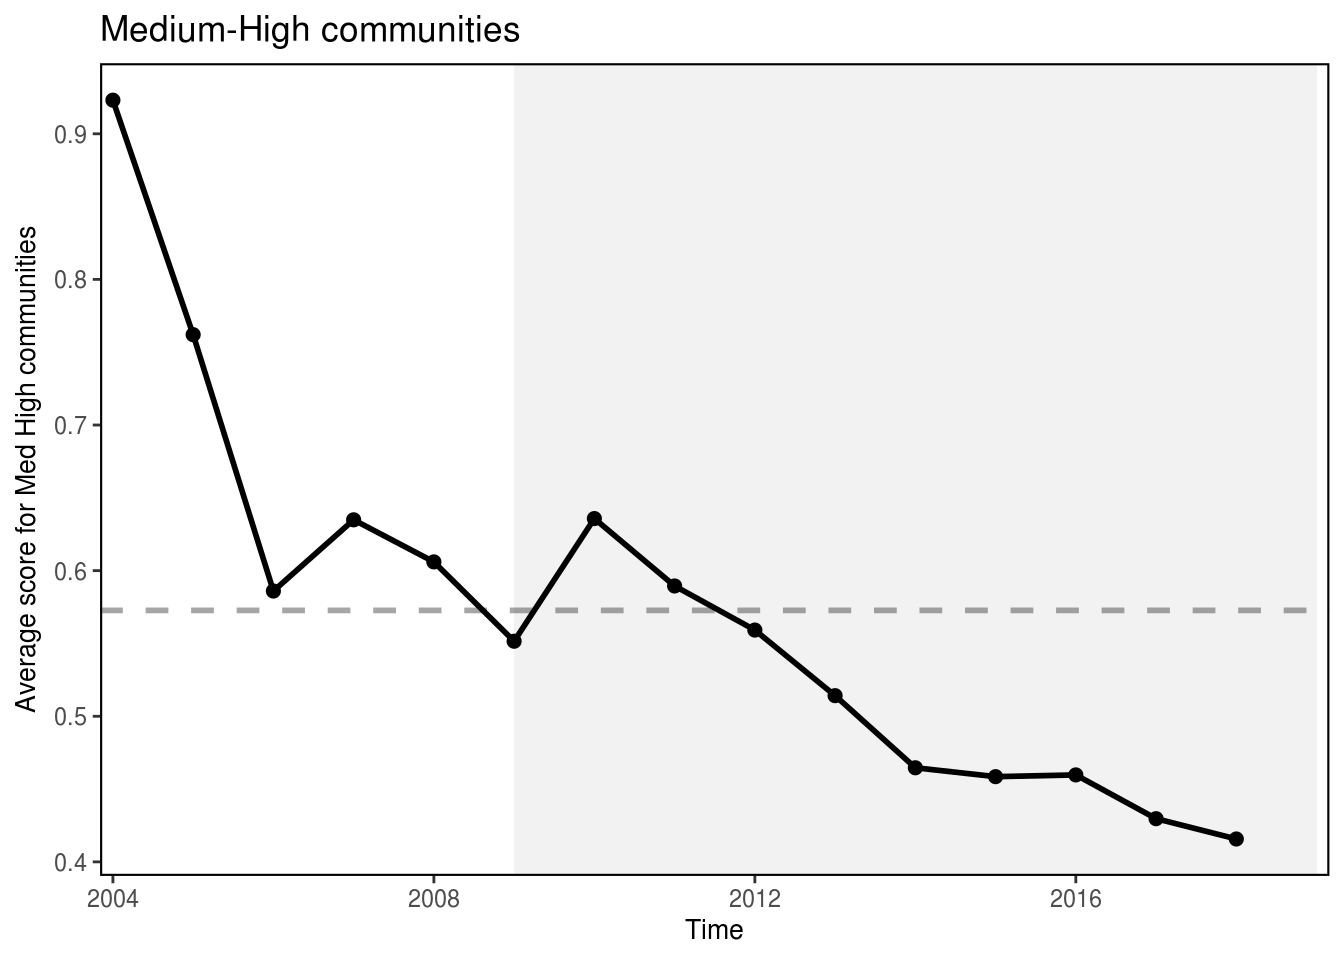
\includegraphics{/home/travis/build/NOAA-EDAB/tech-doc/images/unnamed-chunk-13-2.pdf}

\hypertarget{conceptual-models}{%
\chapter{Conceptual Models}\label{conceptual-models}}

\textbf{Description}: Conceptual models for the New England (Georges Bank and Gulf of Maine) and Mid-Atlantic regions of the Northeast US Large Marine Ecosystem

\textbf{Found in}: State of the Ecosystem - Gulf of Maine \& Georges Bank (2018, 2019, 2020), State of the Ecosystem - Mid-Atlantic (2018, 2019, 2020)

\textbf{Indicator category}: Synthesis of published information, Extensive analysis; not yet published

\textbf{Contributor(s)}: Sarah Gaichas, Patricia Clay, Geret DePiper, Gavin Fay, Michael Fogarty, Paula Fratantoni, Robert Gamble, Sean Lucey, Charles Perretti, Patricia Pinto da Silva, Vincent Saba, Laurel Smith, Jamie Tam, Steve Traynor, Robert Wildermuth

\textbf{Data steward}: Sarah Gaichas, \href{mailto:sarah.gaichas@noaa.gov}{\nolinkurl{sarah.gaichas@noaa.gov}}

\textbf{Point of contact}: Sarah Gaichas, \href{mailto:sarah.gaichas@noaa.gov}{\nolinkurl{sarah.gaichas@noaa.gov}}

\textbf{Public availability statement}: All source data aside from confidential commercial fisheries data (relevant only to some components of the conceptual models) are available to the public (see Data Sources below).

\hypertarget{methods-12}{%
\section{Methods}\label{methods-12}}

Conceptual models were constructed to facilitate multidisciplinary analysis and discussion of the linked social-ecological system for integrated ecosystem assessment. The overall process was to first identify the components of the model (focal groups, human activities, environmental drivers, and objectives), and then to document criteria for including groups and linkages and what the specific links were between the components.

The prototype conceptual model used to design Northeast US conceptual models for each ecosystem production unit (EPU) was designed by the California Current IEA program. The California Current IEA developed an \href{https://www.integratedecosystemassessment.noaa.gov/regions/california-current/cc-ecosystem-components}{overview conceptual model for the Northern California Current Large Marine Ecosystem (NCC)}, with models for each \href{https://www.integratedecosystemassessment.noaa.gov/regions/california-current/cc-coastalpelagicspecies\#overview}{focal ecosystem component} that detailed the \href{https://www.integratedecosystemassessment.noaa.gov/regions/california-current/cc-coastalpelagicspecies\#ecologicalinteractions}{ecological}, \href{https://www.integratedecosystemassessment.noaa.gov/regions/california-current/cc-coastalpelagicspecies\#environmentalDrivers}{environmental}, and \href{https://www.integratedecosystemassessment.noaa.gov/regions/california-current/cc-coastalpelagicspecies\#humanActivities}{human system} linkages. Another set of conceptual models outlined \href{https://www.integratedecosystemassessment.noaa.gov/regions/california-current/cc-habitat}{habitat} linkages.

An inital conceptual model for Georges Bank and the Gulf of Maine was outlined at the 2015 ICES WGNARS meeting. It specified four categories: Large scale drivers, focal ecosystem components, human activities, and human well being. Strategic management objectives were included in the conceptual model, which had not been done in the NCC. Focal ecosystem components were defined as aggregate species groups that had associated US management objectives (outlined within WGNARS for IEAs, see DePiper et al. (\protect\hyperlink{ref-depiper_operationalizing_2017}{2017})): groundfish, forage fish, fished invertebrates, living habitat, and protected species. These categories roughly align with Fishery Managment Plans (FMPs) for the New England Fishery Management Council. The Mid-Atlantic conceptual model was developed along similar lines, but the focal groups included demersals, forage fish, squids, medium pelagics, clams/quahogs, and protected species to better align with the Mid Atlantic Council's FMPs.

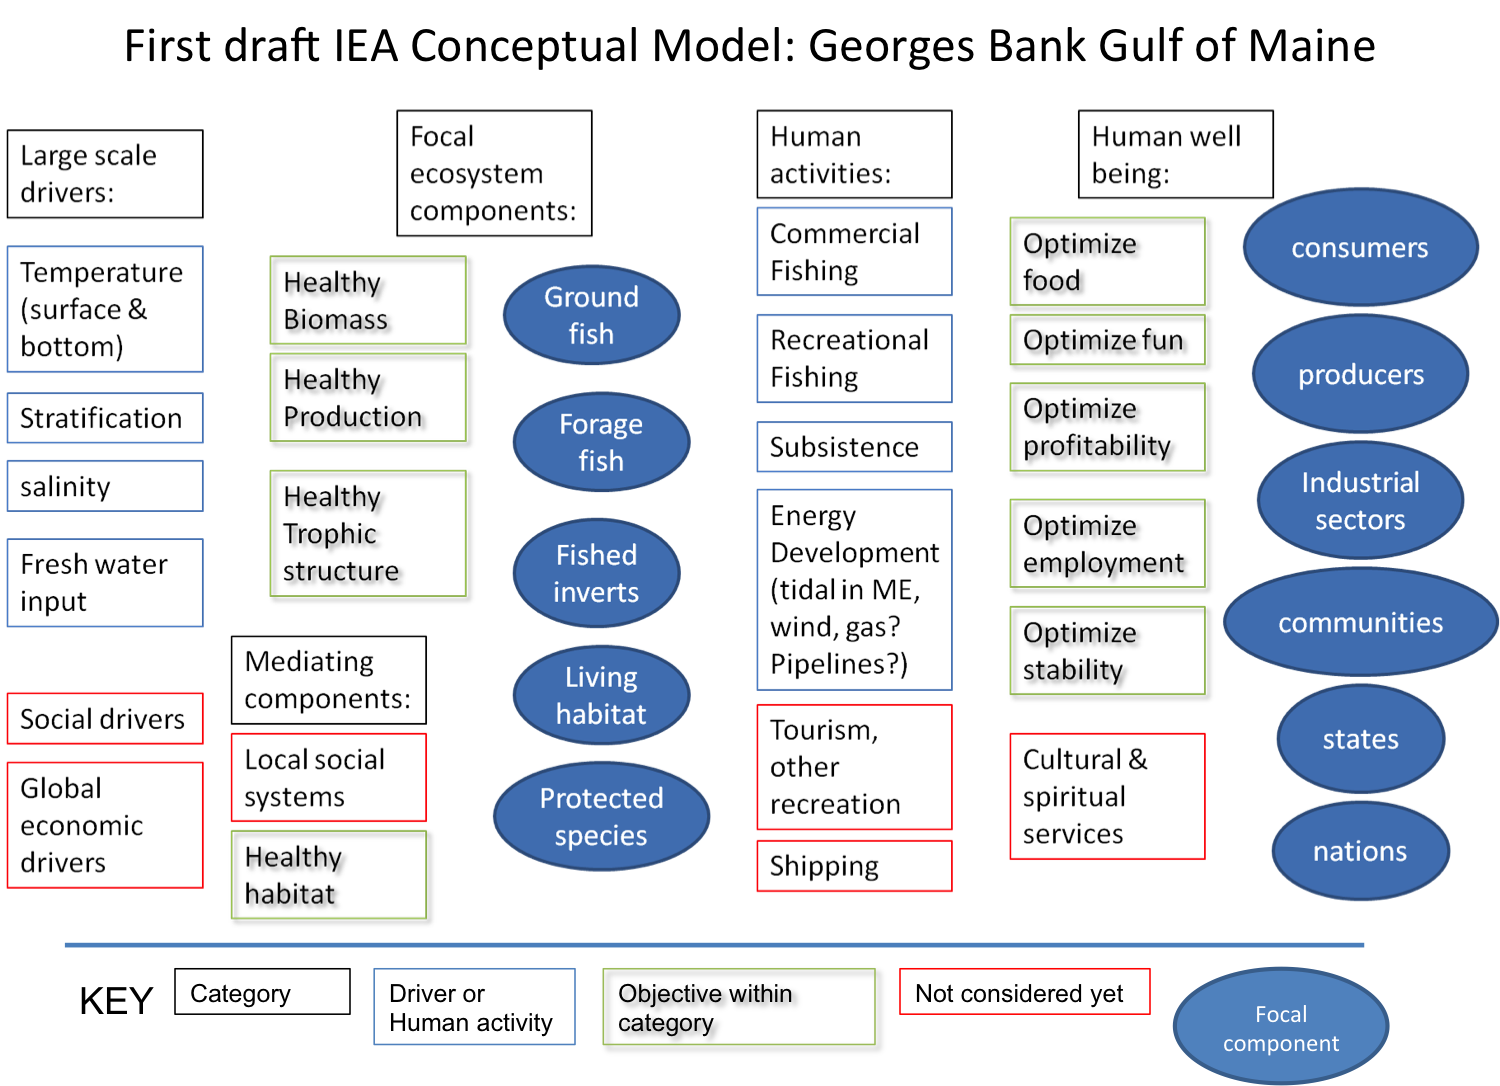
\includegraphics[width=0.8\linewidth]{/home/travis/build/NOAA-EDAB/tech-doc/images/GBGOMconceptual1}

After the initial draft model was outlined, working groups were formed to develop three submodels following the CCE example: ecological, environmental, and human dimensions. The general approach was to specify what was being included in each group, what relationship was represented by a link between groups, what threshold of the relationship was used to determine whether a relationship was significant enough to be included (we did not want to model everything), the direction and uncertainty of the link, and documentation supporting the link between groups. This information was recorded in a \href{https://comet.nefsc.noaa.gov/erddap/tabledap/concept_model_2018.html}{spreadsheet}. Submodels were then merged together by common components using the ``merge'' function in the (currently unavailable) desktop version of Mental Modeler (\url{http://www.mentalmodeler.org/\#home}; Gray et al. (\protect\hyperlink{ref-gray_mental_2013}{2013})). The process was applied to Georges Bank (GB), the Gulf of Maine (GOM), and the Mid-Atlantic Bight (MAB) \protect\hyperlink{epu}{Ecological Production Units}.

\hypertarget{data-sources-12}{%
\subsection{Data sources}\label{data-sources-12}}

\hypertarget{ecological-submodels}{%
\subsubsection{Ecological submodels}\label{ecological-submodels}}

Published food web (EMAX) models for each subregion (J. S. Link et al. \protect\hyperlink{ref-link_documentation_2006}{2006}; Link et al. \protect\hyperlink{ref-link_northeast_2008}{2008}), food habits data collected by NEFSC trawl surveys (Smith and Link \protect\hyperlink{ref-smith_trophic_2010}{2010}), and other literature sources (Smith et al. \protect\hyperlink{ref-smith_consumption_2015}{2015}) were consulted. Expert judgement was also used to adjust historical information to current conditions, and to include broad habitat linkages to Focal groups.

\hypertarget{environmental-submodels}{%
\subsubsection{Environmental submodels}\label{environmental-submodels}}

Published literature on the primary environmental drivers (seasonal and interannual) in each EPU was consulted.
Sources for Georges Bank included Backus and Bourne (\protect\hyperlink{ref-backus_georges_1987}{1987}) and Townsend et al. (\protect\hyperlink{ref-townsend_oceanography_2006}{2006}).
Sources for the Gulf of Maine included Smith (\protect\hyperlink{ref-smith_mean_1983}{1983}), Smith et al. (\protect\hyperlink{ref-smith_interannual_2001}{2001}), Mupparapu and Brown (\protect\hyperlink{ref-mupparapu_role_2002}{2002}), Townsend et al. (\protect\hyperlink{ref-townsend_oceanography_2006}{2006}), Smith et al. (\protect\hyperlink{ref-smith_regime_2012}{2012}), and Mountain (\protect\hyperlink{ref-mountain_labrador_2012}{2012}).\\
Sources for the Mid Atlantic Bight included Houghton et al. (\protect\hyperlink{ref-houghton_middle_1982}{1982}), Beardsley et al. (\protect\hyperlink{ref-beardsley_nantucket_1985}{1985}), Lentz (\protect\hyperlink{ref-lentz_climatology_2003}{2003}), Mountain (\protect\hyperlink{ref-mountain_variability_2003}{2003}), Glenn et al. (\protect\hyperlink{ref-glenn_biogeochemical_2004}{2004}), Sullivan, Cowen, and Steves (\protect\hyperlink{ref-sullivan_evidence_2005}{2005}), Castelao et al. (\protect\hyperlink{ref-castelao_seasonal_2008}{2008}), Shearman and Lentz (\protect\hyperlink{ref-shearman_long-term_2009}{2009}), Castelao, Glenn, and Schofield (\protect\hyperlink{ref-castelao_temperature_2010}{2010}), Gong, Kohut, and Glenn (\protect\hyperlink{ref-gong_seasonal_2010}{2010}), Gawarkiewicz et al. (\protect\hyperlink{ref-gawarkiewicz_direct_2012}{2012}), Forsyth, Andres, and Gawarkiewicz (\protect\hyperlink{ref-forsyth_recent_2015}{2015}), Fratantoni, Holzwarth-Davis, and Taylor (\protect\hyperlink{ref-fratantoni_description_2015}{2015}), Zhang and Gawarkiewicz (\protect\hyperlink{ref-zhang_dynamics_2015}{2015}), Timothy J. Miller, Hare, and Alade (\protect\hyperlink{ref-miller_state-space_2016}{2016}), and Lentz (\protect\hyperlink{ref-lentz_seasonal_2017}{2017}).

\hypertarget{human-dimensions-submodels}{%
\subsubsection{Human dimensions submodels}\label{human-dimensions-submodels}}

Fishery catch and bycatch information was drawn from multiple regional datasets, incuding the Greater Atlantic Regional Office Vessel Trip Reports \& Commercial Fisheries Dealer databases, Northeast Fishery Observer Program \& Northeast At-Sea Monitoring databases, Northeast Fishery Science Center Social Sciences Branch cost survey, and the Marine Recreational Informational Program database. Further synthesis of human welfare derived from fisheries was drawn from Färe, Kirkley, and Walden (\protect\hyperlink{ref-fare_adjusting_2006}{2006}), Walden et al. (\protect\hyperlink{ref-walden_productivity_2012}{2012}), Lee and Thunberg (\protect\hyperlink{ref-lee_inverse_2013}{2013}), Lee (\protect\hyperlink{ref-lee_hedonic_2014}{2014}), and Lee, Steinback, and Wallmo (\protect\hyperlink{ref-lee_applying_2017}{2017}). Bycatch of protected species was taken from Waring et al. (\protect\hyperlink{ref-waring_us_2015}{2015}), with additional insights from Bisack and Magnusson (\protect\hyperlink{ref-bisack_measuring_2014}{2014}). The top 3 linkages were drawn for each node. For example, the top 3 recreational species for the Mid-Atlantic were used to draw linkages between the recreational fishery and species focal groups. A similar approach was used for relevant commercial fisheries in each region.

Habitat-fishery linkages were drawn from unpublished reports, including:

\begin{enumerate}
\def\labelenumi{\arabic{enumi}.}
\item
  Mid-Atlantic Fishery Management Council. 2016. \href{http://www.mafmc.org/actions/msb-am16}{Amendment 16} to the Atlantic Mackerel, Squid, and Butterfish Fishery Management Plan: Measures to protect deep sea corals from Impacts of Fishing Gear. Environmental Assessment, Regulatory Impact Review, and Initial Regulatory Flexibility Analysis. Dover, DE. August, 2016.
\item
  NOAA. 2016. Deep sea coral research and technology program 2016 Report to Congress. \url{http://www.habitat.noaa.gov/protection/corals/deepseacorals.html} retrieved February 8, 2017.
\item
  New England Fishery Management Council. 2016. Habitat Omnibus Deep-Sea Coral Amendment: Draft. \url{http://www.nefmc.org/library/omnibus-deep-sea-coral-amendment} Retrieved Feb 8, 2017.
\item
  Bachman et al.~2011. The Swept Area Seabed Impact (SASI) Model: A Tool for Analyzing the Effects of Fishing on Essential Fish Habitat. New England Fisheries Management Council Report. Newburyport, MA.
\end{enumerate}

Tourism and habitat linkages were drawn from unpublished reports, including:

\begin{enumerate}
\def\labelenumi{\arabic{enumi}.}
\item
  \url{http://neers.org/RESOURCES/Bibliographies.html}
\item
  Great Bay (GoM) resources \url{http://greatbay.org/about/publications.htm}
\item
  Meaney, C.R. and C. Demarest. 2006. Coastal Polution and New England Fisheries. Report for the New England Fisheries Management Council. Newburyport, MA.
\item
  List of valuation studies, by subregion and/or state, can be found at \url{http://www.oceaneconomics.org/nonmarket/valestim.asp}.
\end{enumerate}

Published literature on human activities in each EPU was consulted.

Sources for protected species and tourism links included Hoagland and Meeks (\protect\hyperlink{ref-hoagland_demand_2000}{2000}) and Lee (\protect\hyperlink{ref-lee_economic_2010}{2010}).

Sources for links between environmental drivers and human activities included Adams (\protect\hyperlink{ref-adams_uncertainty_1973}{1973}), Matzarakis and Freitas (\protect\hyperlink{ref-matzarakis_proceedings_2001}{2001}), Scott, McBoyle, and Schwartzentruber (\protect\hyperlink{ref-scott_climate_2004}{2004}), Hess, Malilay, and Parkinson (\protect\hyperlink{ref-hess_climate_2008}{2008}), L. L. Colburn and Jepson (\protect\hyperlink{ref-colburn_social_2012}{2012}\protect\hyperlink{ref-colburn_social_2012}{b}), Jepson and Colburn (\protect\hyperlink{ref-jepson_development_2013}{2013}), and Colburn et al. (\protect\hyperlink{ref-colburn_indicators_2016}{2016}).

Sources for cultural practices and attachments links included Pauly (\protect\hyperlink{ref-pauly_putting_1997}{1997}), McGoodwin (\protect\hyperlink{ref-mcgoodwin_understanding_2001}{2001}), St Martin (\protect\hyperlink{ref-st_martin_making_2001}{2001}), Norris-Raynbird (\protect\hyperlink{ref-norris-raynbird_for_2004}{2004}), Pollnac et al. (\protect\hyperlink{ref-pollnac_toward_2006}{2006}), Clay and Olson (\protect\hyperlink{ref-clay_defining_2007}{2007}), Clay and Olson (\protect\hyperlink{ref-clay_definingfishing_2008}{2008}), Everett and Aitchison (\protect\hyperlink{ref-everett_role_2008}{2008}), Donkersloot (\protect\hyperlink{ref-donkersloot_politics_2010}{2010}), Lord (\protect\hyperlink{ref-lord_understanding_2011}{2011}), Halpern et al. (\protect\hyperlink{ref-halpern_index_2012}{2012}), Wynveen, Kyle, and Sutton (\protect\hyperlink{ref-wynveen_natural_2012}{2012}), Cortes-Vazquez and Zedalis (\protect\hyperlink{ref-cortes-vazquez_identity_2013}{2013}), Koehn, Reineman, and Kittinger (\protect\hyperlink{ref-koehn_progress_2013}{2013}), Potschin and Haines-Young (\protect\hyperlink{ref-potschin_landscapes_2013}{2013}), Reed et al. (\protect\hyperlink{ref-reed_beyond_2013}{2013}), Urquhart and Acott (\protect\hyperlink{ref-urquhart_constructing_2013}{2013}), Blasiak et al. (\protect\hyperlink{ref-blasiak_paradigms_2014}{2014}), Klain, Satterfield, and Chan (\protect\hyperlink{ref-klain_what_2014}{2014}), Poe, Norman, and Levin (\protect\hyperlink{ref-poe_cultural_2014}{2014}), Brown (\protect\hyperlink{ref-brown_we_2015}{2015}), Donatuto and Poe (\protect\hyperlink{ref-donatuto_evaluating_2015}{2015}), Khakzad and Griffith (\protect\hyperlink{ref-khakzad_role_2016}{2016}), Oberg et al. (\protect\hyperlink{ref-oberg_surviving_2016}{2016}), and Seara, Clay, and Colburn (\protect\hyperlink{ref-seara_perceived_2016}{2016}).

\hypertarget{data-extraction-11}{%
\subsection{Data extraction}\label{data-extraction-11}}

\hypertarget{ecological-submodels-1}{%
\subsubsection{Ecological submodels}\label{ecological-submodels-1}}

``Data'' included model estimated quantities to determine whether inclusion thresholds were met for each potential link in the conceptual model. A matrix with diet composition for each modeled group is an input to the food web model. A matrix of mortalities caused by each predator and fishery on each modeled group is a direct ouput of a food web model (e.g.~Ecopath). Food web model biomasss flows between species, fisheries, and detritus were summarized using algorithms implemented in visual basic by Kerim Aydin, NOAA NMFS Alaska Fisheries Science Center. Because EMAX model groups were aggregated across species, selected diet compositions for individual species were taken from the NEFSC food habits database using the FEAST program for selected species (example query below). These diet queries were consulted as supplemental information.

Example FEAST sql script for Cod weighted diet on Georges Bank can be found \href{https://github.com/NOAA-EDAB/tech-doc/tree/master/R/stored_scripts/conceptual_models_extraction.sql}{here}.
Queries for different species are standardized by the FEAST application and would differ only in the svspp code.

\hypertarget{environmental-submodels-1}{%
\subsubsection{Environmental submodels}\label{environmental-submodels-1}}

Information was synthesized entirely from published sources and expert knowledge; no additional data extraction was completed for the environmental submodels.

\hypertarget{human-dimensions-submodels-1}{%
\subsubsection{Human dimensions submodels}\label{human-dimensions-submodels-1}}

Recreational fisheries data were extracted from the 2010-2014 MRIP datasets. Original data can be found \href{data/top10_prim1_common_mode.xlsx}{here} for each region (New England or Mid-Atlantic as defined by states).

Commercial fishing data was developed as part of the State of the Ecosystem Report, including revenue and food production estimates, with data extraction metodology discussed in the relevant sections of the technical document. In addition, the Northeast Regional Input/Output Model (Steinback and Thunberg \protect\hyperlink{ref-steinback_scott_northeast_2006}{2006}) was used as the basis for the strength of the employment linkages.

\hypertarget{data-analysis-11}{%
\subsection{Data analysis}\label{data-analysis-11}}

\hypertarget{ecological-submodels-2}{%
\subsubsection{Ecological submodels}\label{ecological-submodels-2}}

Aggregated diet and mortality information was examined to determine the type of link, direction of link, and which links between which groups should be inclded in the conceptual models. Two types of ecological links were defined using food web models: prey links and predation/fishing mortality links. Prey links resulted in positve links between the prey group and the focal group, while predation/fishing mortality links resulted in negative links to the focal group to represent energy flows. The intent was to include only the most important linkages between focal groups and with other groups supporting or causing mortality on focal species groups. Therefore, threshold levels of diet and mortality were established (based on those that would select the top 1-3 prey and predators of each focal group): 10\% to include a link (or add a linked group) in the model and 20\% to include as a strong link. A Primary Production group was included in each model and linked to pelagic habitat to allow environmental effects on habitat to be connected to the ecologial submodel. Uncertainty for the inclusion of each link and for the magnitude of each link was qualitatively assessed and noted in the \href{https://comet.nefsc.noaa.gov/erddap/tabledap/concept_model_2018.html}{spreadsheet}.

Four habitat categories (Pelagic, Seafloor and Demersal, Nearshore, and Freshwater and Estuarine) were included in ecological submodels as placeholders to be developed further along with habitat-specific research. Expert opinion was used to include the strongest links between each habitat type and each Focal group (noting that across species and life stages, members of these aggregate groups likely occupy many if not all of the habitat types). Link direction and strength were not specified. Environmental drivers were designed to link to habitats, rather than directly to Focal groups, to represent each habitat's important mediation function.

EMAX model groups were aggregated to focal groups for the Georges Bank (GB), Gulf of Maine (GOM) and Mid-Atlantic Bight (MAB) conceptual models according to Table \ref{tab:groups}. ``Linked groups'' directly support or impact the Focal groups as described above.

\begin{landscape}\begin{table}

\caption{\label{tab:groups}Relationship between food web model groups and conceptual model focal groups. Pinnipeds not included in GB and Seabirds not included in MAB.}
\centering
\fontsize{8}{10}\selectfont
\begin{tabular}[t]{llll}
\toprule
Group Type & Region & Conceptual model group & EMAX group(s)\\
\midrule
Focal & GB & Commercial Fishery & Fishery\\
Focal & GB & Fished Inverts & Megabenthos filterers\\
Focal & GB & Forage Fish & Sum of Small pelagics-commercial, other, anadromous, and squids\\
Focal & GB & Groundfish & Sum of Demersals-omnivores, benthivores, and piscivores\\
Focal & GB & Protected Species & Sum of Baleen Whales, Odontocetes, and Seabirds\\
\addlinespace
Linked & GB & Benthos & Sum of Macrobenthos-polychaetes, crustaceans, molluscs, other and Megabenthos-other\\
Linked & GB & Copepods and Micronecton & Sum of Copepods-small and large, and Micronekton\\
Linked & GB & Detritus and Bacteria & Sum of Bacteria and Detritus-POC\\
Linked & GB & Gelatinous zooplankton & Gelatinous zooplankton\\
Linked & GB & Primary Production & Phytoplankton-Primary production\\
\addlinespace
Focal & GOM & Commercial Fishery & Fishery\\
Focal & GOM & Fished Inverts & Megabenthos filterers\\
Focal & GOM & Forage Fish & Sum of Small pelagics-commercial, other, anadromous, and squids\\
Focal & GOM & Groundfish & Sum of Demersals-omnivores, benthivores, and piscivores\\
Focal & GOM & Protected Species & Sum of Baleen Whales, Odontocetes, Pinnipeds, and Seabirds\\
\addlinespace
Linked & GOM & Benthos & Sum of Macrobenthos-polychaetes, crustaceans, molluscs, other and Megabenthos-other\\
Linked & GOM & Copepods and Micronecton & Sum of Copepods-small and large, and Micronekton\\
Linked & GOM & Detritus and Bacteria & Sum of Bacteria and Detritus-POC\\
Linked & GOM & Gelatinous zooplankton & Gelatinous zooplankton\\
Linked & GOM & Primary Production & Phytoplankton-Primary production\\
\addlinespace
Focal & MAB & Clams Quahogs & Megabenthos filterers\\
Focal & MAB & Commercial Fishery & Fishery\\
Focal & MAB & Demerals & Sum of Demersals-omnivores, benthivores, and piscivores\\
Focal & MAB & Forage Fish & Sum of Small pelagics-commercial, other, and anadromous\\
Focal & MAB & Medium Pelagics & Medium pelagics\\
\addlinespace
Focal & MAB & Protected Species & Sum of Baleen whales and Odontocetes\\
Focal & MAB & Squids & Small pelagics-squids\\
Linked & MAB & Benthos & Sum of Macrobenthos-polychaetes, crustaceans, molluscs, other\\
Linked & MAB & Copepods and Micronecton & Sum of Copepods-small and large, and Micronekton\\
Linked & MAB & Detritus and Bacteria & Sum of Bacteria and Detritus-POC\\
\addlinespace
Linked & MAB & Gelatinous zooplankton & Gelatinous zooplankton\\
Linked & MAB & Primary Production & Phytoplankton-Primary production\\
Linked & MAB & Sharks & Sum of Sharks-pelagic and coastal\\
\bottomrule
\end{tabular}
\end{table}
\end{landscape}

Ecological submodels were constructed and visualized in Mental Modeler (Fig. \ref{fig:draftGOMeco}). Here, we show only the Gulf of Maine submodels as examples.

\begin{figure}
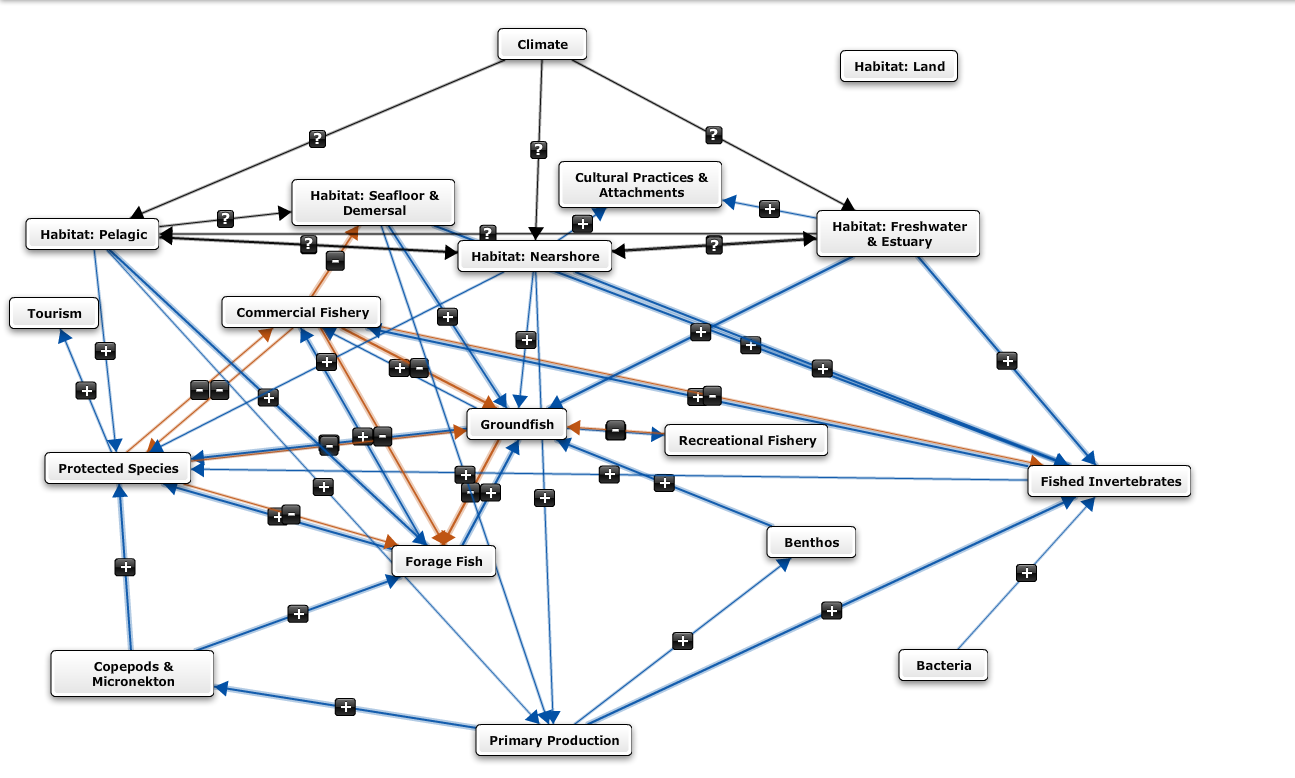
\includegraphics[width=0.8\linewidth]{/home/travis/build/NOAA-EDAB/tech-doc/images/MM_GoM_Ecological} \caption{Gulf of Maine Ecological submodel}\label{fig:draftGOMeco}
\end{figure}

\hypertarget{environmental-submodels-2}{%
\subsubsection{Environmental submodels}\label{environmental-submodels-2}}

Environmental submodels were designed to link key oceanographic processes in each ecosystem production unit to the four general habitat categories (Pelagic, Seafloor and Demersal, Nearshore, and Freshwater and Estuarine) with emphasis on the most important physical processes in each ecosystem based on expert knowledge as supported by literature review. The basis of each submodel were environmental variables observable at management-relevant scales as identified by \href{http://ices.dk/sites/pub/Publication\%20Reports/Expert\%20Group\%20Report/SSGRSP/2014/WGNARS14.pdf}{WGNARS}: Surface and Bottom Water Temperature and Salinity, Freshwater Input, and Stratification (as well as sea ice timing and cover, which is not relevant to the northeast US shelf). Key drivers changing these observable variables and thus structuring habitat dynamics in each \protect\hyperlink{epu}{Ecological Production Units} were added to the model using expert consensus.

Environmental submodels were initially constructed and visualized in Mental Modeler (Fig. \ref{fig:draftGOMenv}).

\begin{figure}
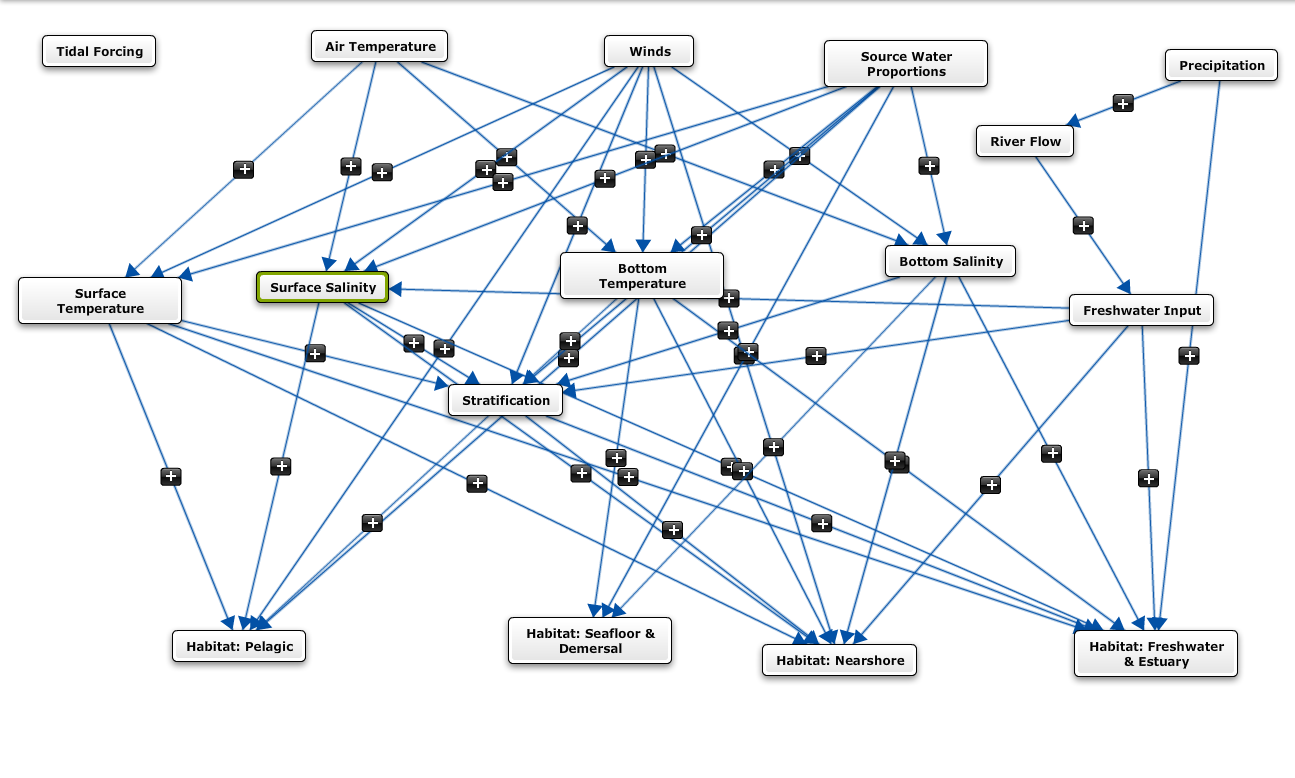
\includegraphics[width=0.8\linewidth]{/home/travis/build/NOAA-EDAB/tech-doc/images/MM_GoM_Climate} \caption{Gulf of Maine Environmental submodel}\label{fig:draftGOMenv}
\end{figure}

\hypertarget{human-dimensions-submodels-2}{%
\subsubsection{Human dimensions submodels}\label{human-dimensions-submodels-2}}

The top 3 species from each mode of recreational fishing (shoreside, private boat, party/charter) were used to assess the potential for missing links between the recreational fishing activity and biological focal components. Given the predominance of Mid-Atlantic groundfish in recreational fishing off New England (summer flounder, bluefish, striped bass), a Mid-Atlantic groundfish focal component was added to the Georges Bank EPU model. The magnitude of benefits generated from recreational fishing was scaled to reflect expert knowledge of target species, coupled with the MRIP data highlighted above. Scales were held consistent across the focal components within recreational fishing.

No additional biological focal components were added to the commercial fishing activity, beyond what was developed in the ecological submodel. Benefits derived from commercial fishing were scaled to be consistent with the State of the Ecosystem revenue estimates, as modulated by expert knowledge and additional data sources. For example,the percentage of landings sold as food was used to map fishing activity to the commercial fishery food production objective, and the Northeast Regional Input/Output Model (Steinback and Thunberg \protect\hyperlink{ref-steinback_scott_northeast_2006}{2006}) was used to define the strength of the employment linkages. For profitability, expert knowledge was used to reweight revenue landings, based on ancillary cost data available (Das, Chhandita \protect\hyperlink{ref-das_chhandita_northeast_2013}{2013}, \protect\hyperlink{ref-das_chhandita_overview_2014}{2014}). Human activities and objectives for the conceptual sub model are defined in DePiper et al. (\protect\hyperlink{ref-depiper_operationalizing_2017}{2017}). As shown in Figure \ref{fig:draftGOMhuman}, human dimensions submodels were also initially constructed and visualized in Mental Modeler.

\begin{figure}
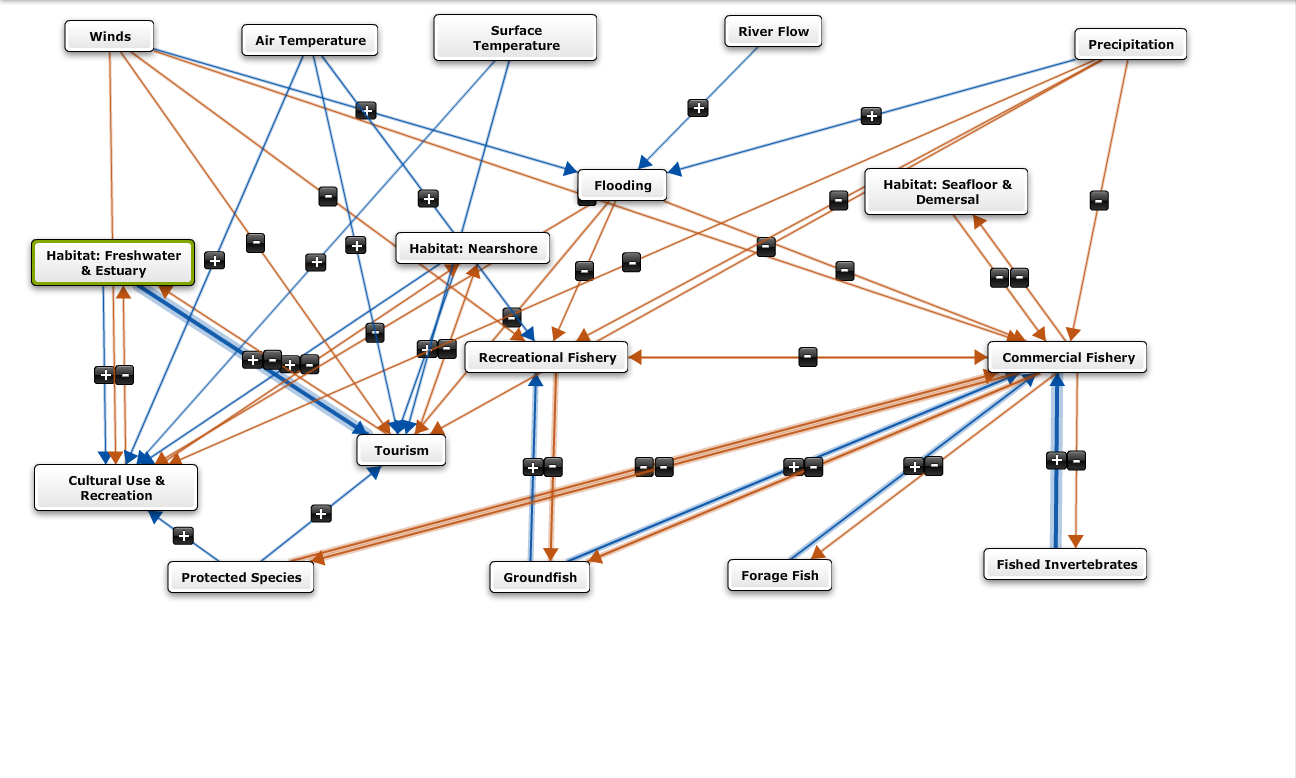
\includegraphics[width=0.8\linewidth]{/home/travis/build/NOAA-EDAB/tech-doc/images/MM_GoM_Human_Connections} \caption{Gulf of Maine Human dimensions submodel}\label{fig:draftGOMhuman}
\end{figure}

\hypertarget{merged-models}{%
\subsubsection{Merged models}\label{merged-models}}

All links and groups from each submodel were preserved in the full merged model for each system. Mental modeler was used to merge the submodels. Full models were then re-drawn in Dia (\url{http://dia-installer.de/}) with color codes for each model component type for improved readability. Examples for each system are below.

\begin{figure}
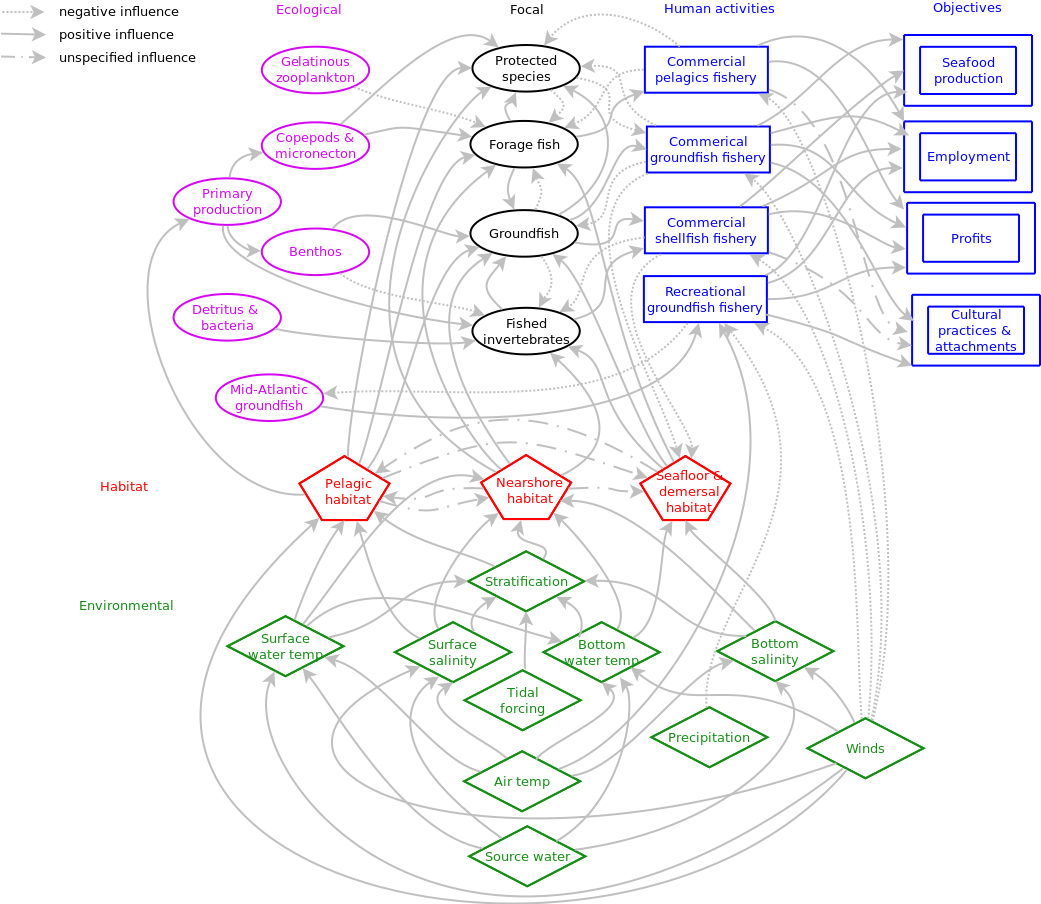
\includegraphics[width=0.8\linewidth]{/home/travis/build/NOAA-EDAB/tech-doc/images/GBoverview5} \caption{Georges Bank conceptual model}\label{fig:diaGB}
\end{figure}

\begin{figure}
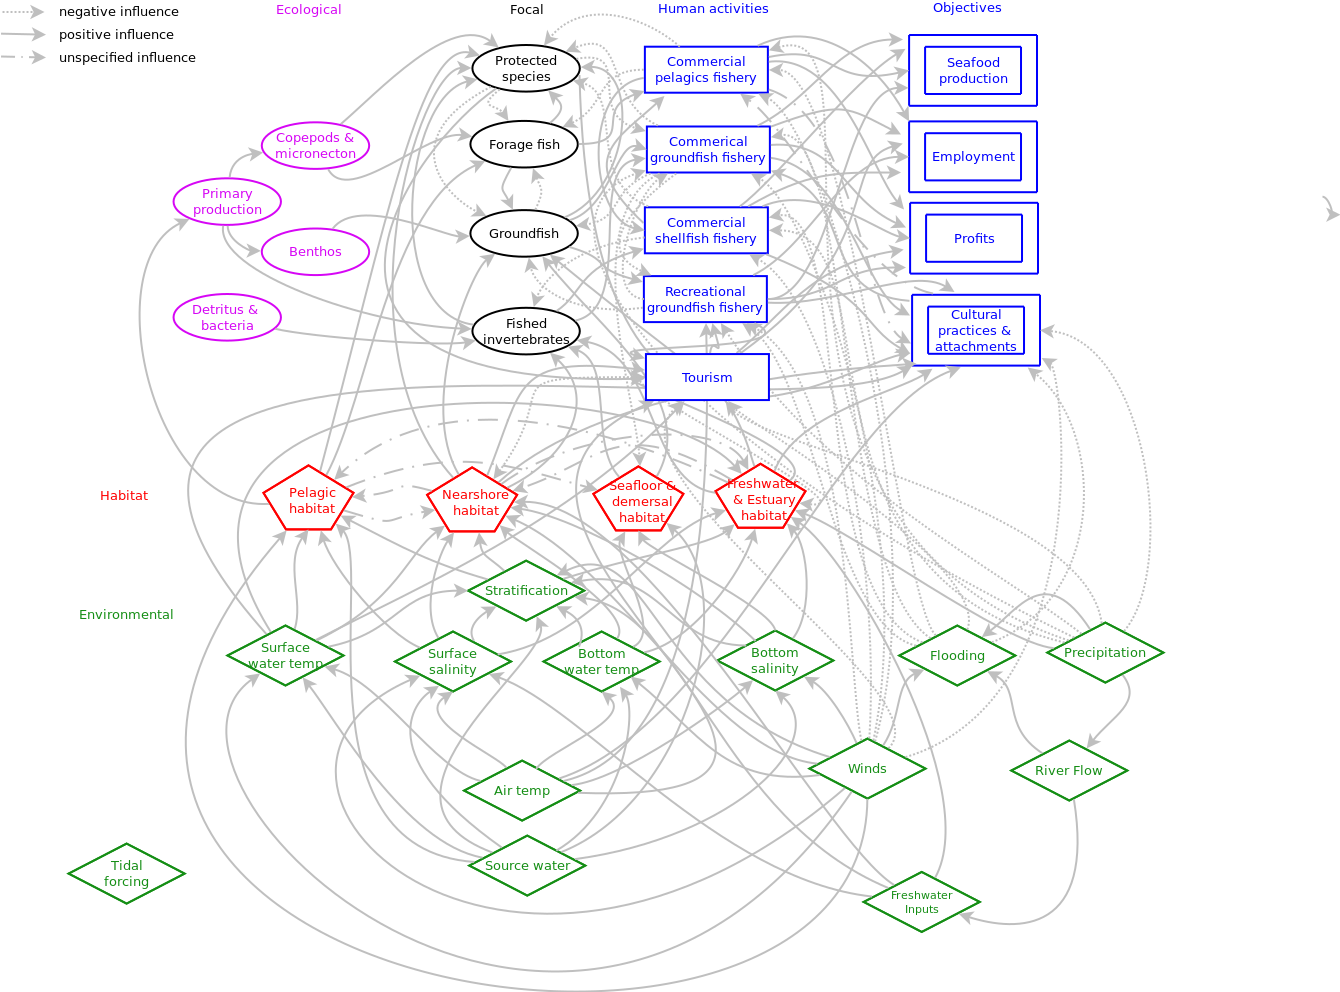
\includegraphics[width=0.8\linewidth]{/home/travis/build/NOAA-EDAB/tech-doc/images/GoMoverview4} \caption{Gulf of Maine conceptual model}\label{fig:diaGOM}
\end{figure}

\begin{figure}
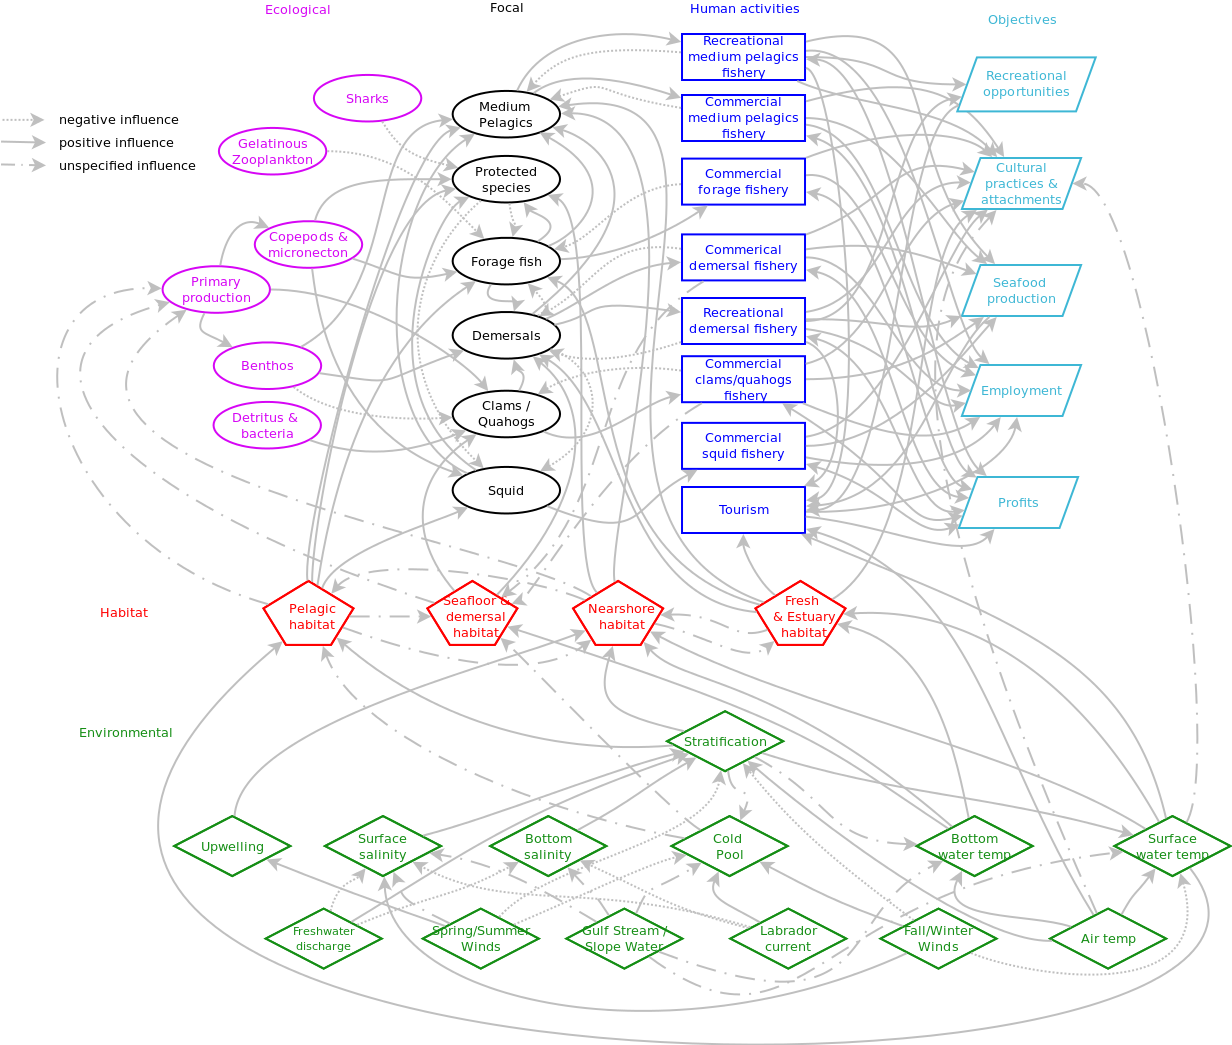
\includegraphics[width=0.8\linewidth]{/home/travis/build/NOAA-EDAB/tech-doc/images/MAB_3} \caption{Mid-Atlantic Bight conceptual model}\label{fig:diaMAB}
\end{figure}

\hypertarget{communication-tools}{%
\subsubsection{Communication tools}\label{communication-tools}}

The merged models were redrawn for use in communications with the public. These versions lead off the State of the Ecosystem reports for both Fishery Management Councils to provide an overview of linkages between environmental drivers, ecological, and human systems.

\begin{figure}
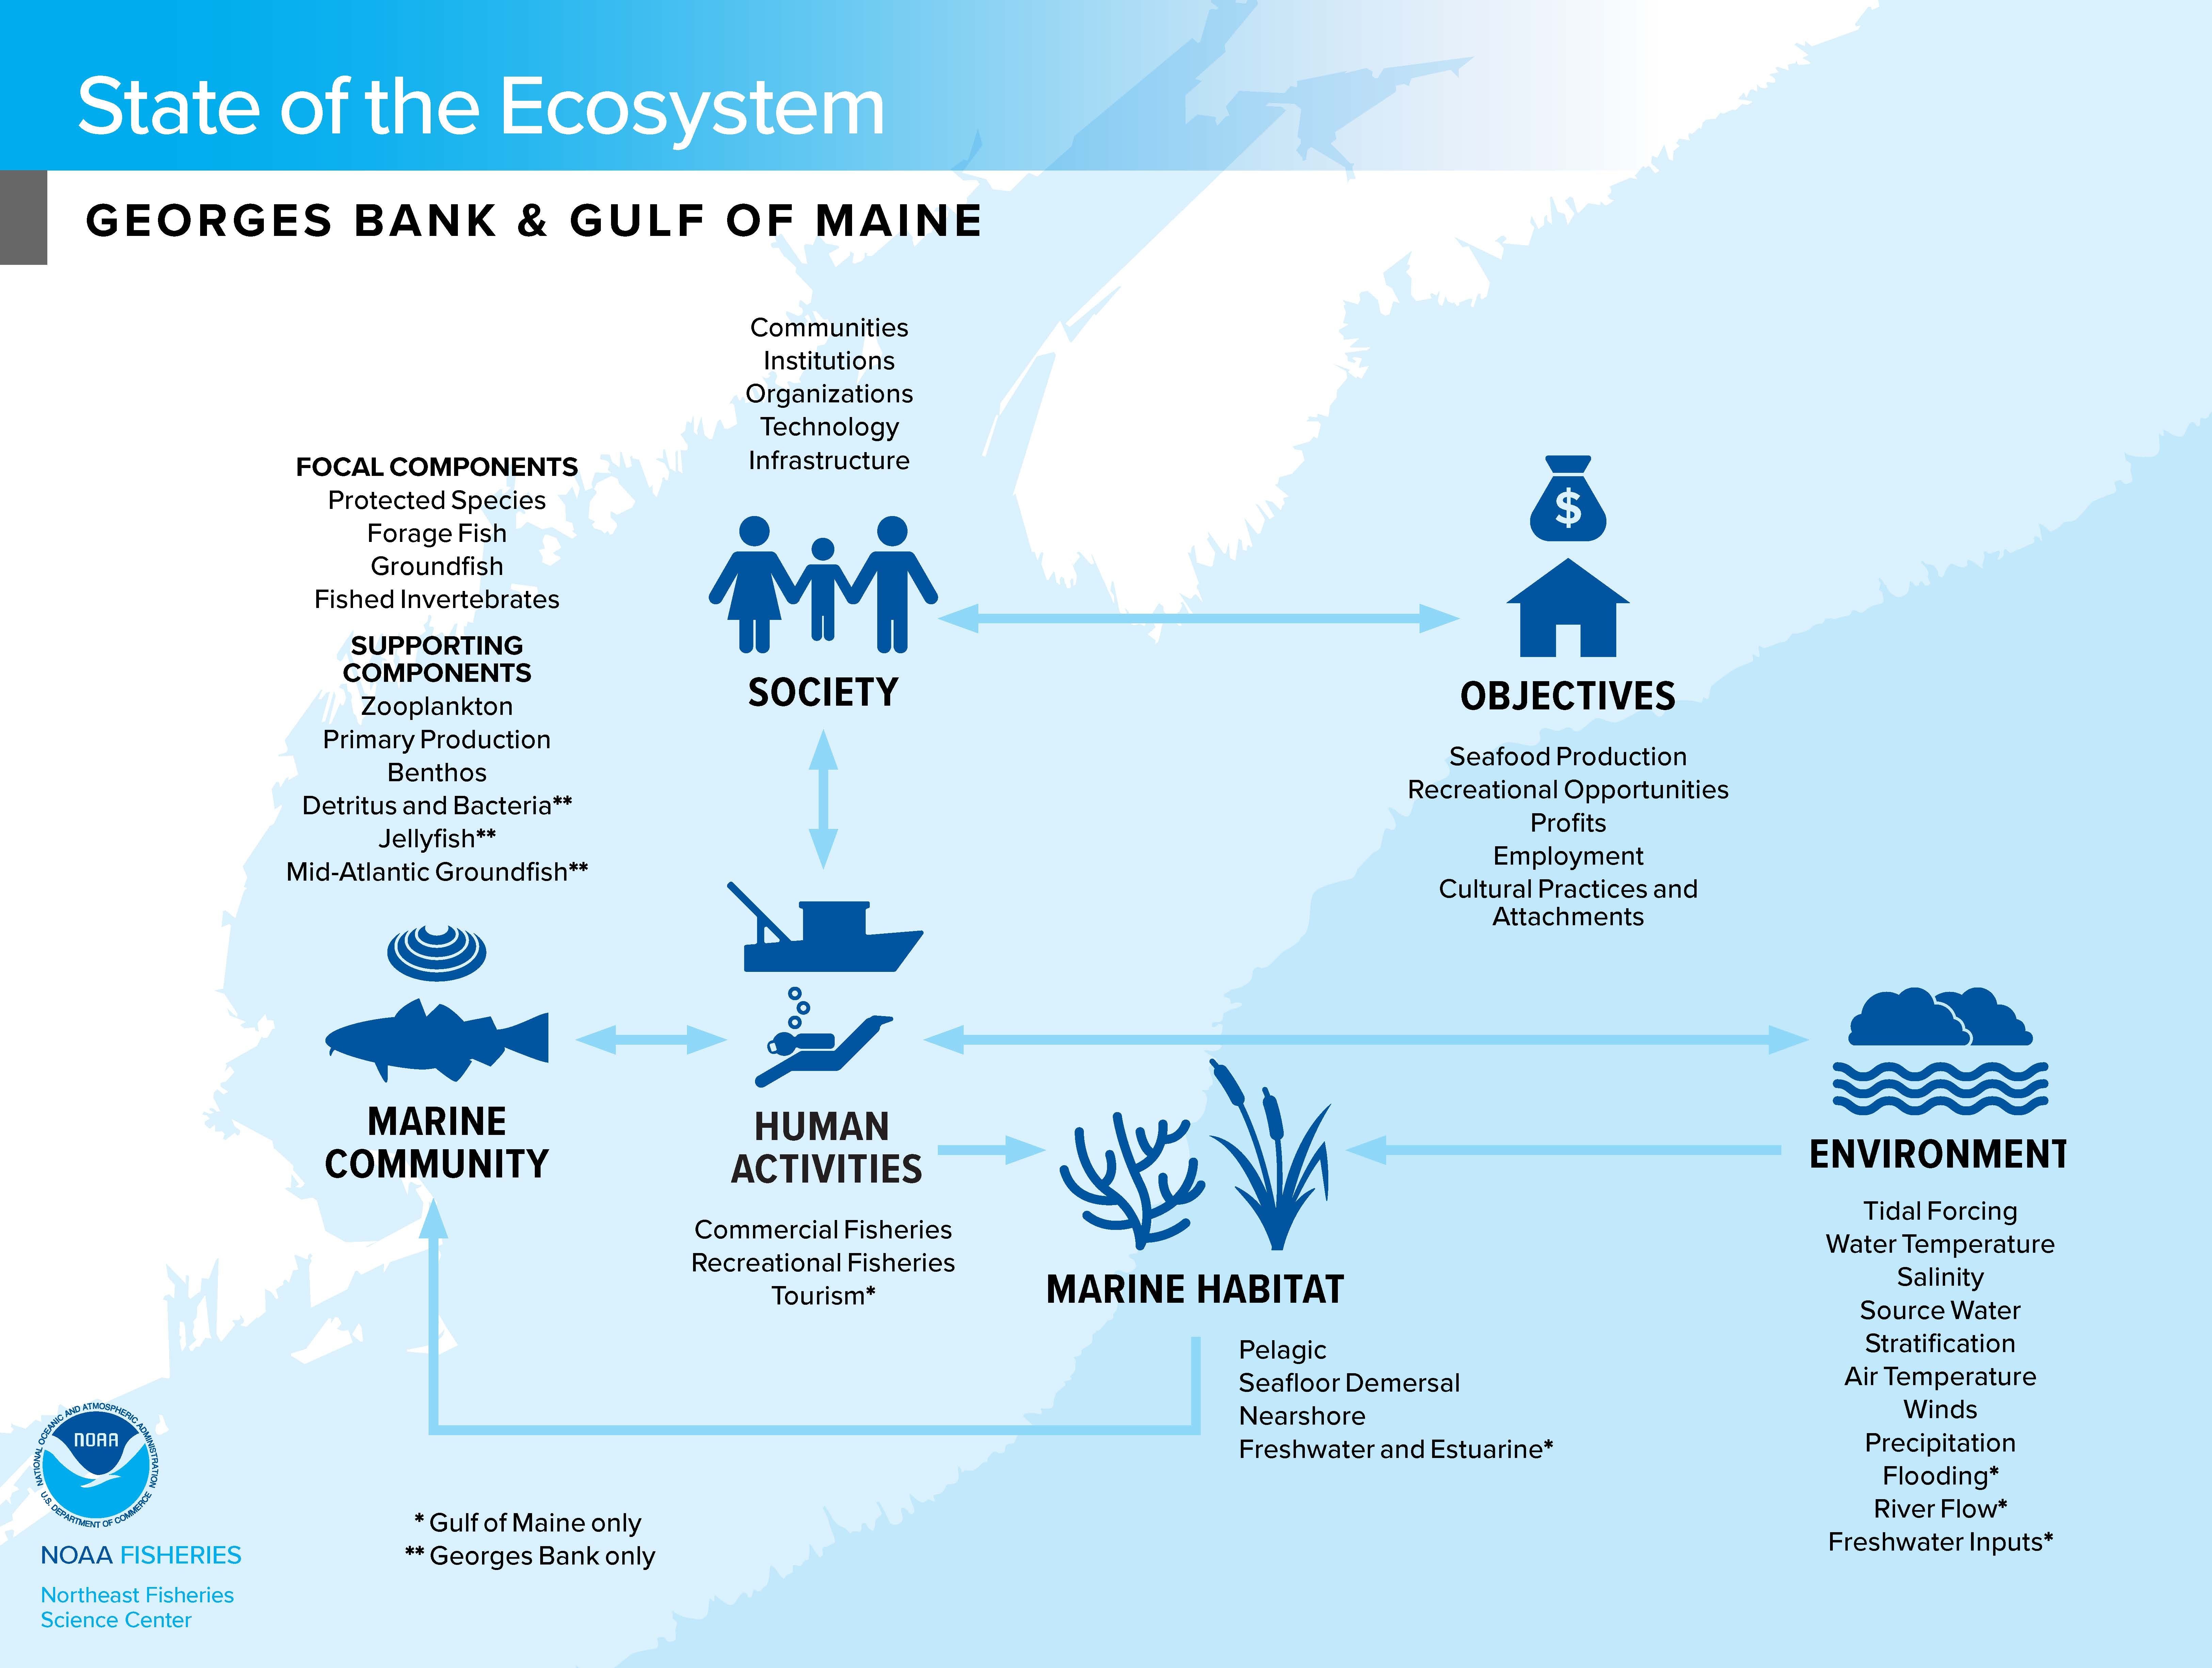
\includegraphics[width=0.8\linewidth]{/home/travis/build/NOAA-EDAB/tech-doc/images/GOM_GB_conmod_overview} \caption{New England conceptual model for public communication}\label{fig:prettyNE}
\end{figure}

\begin{figure}
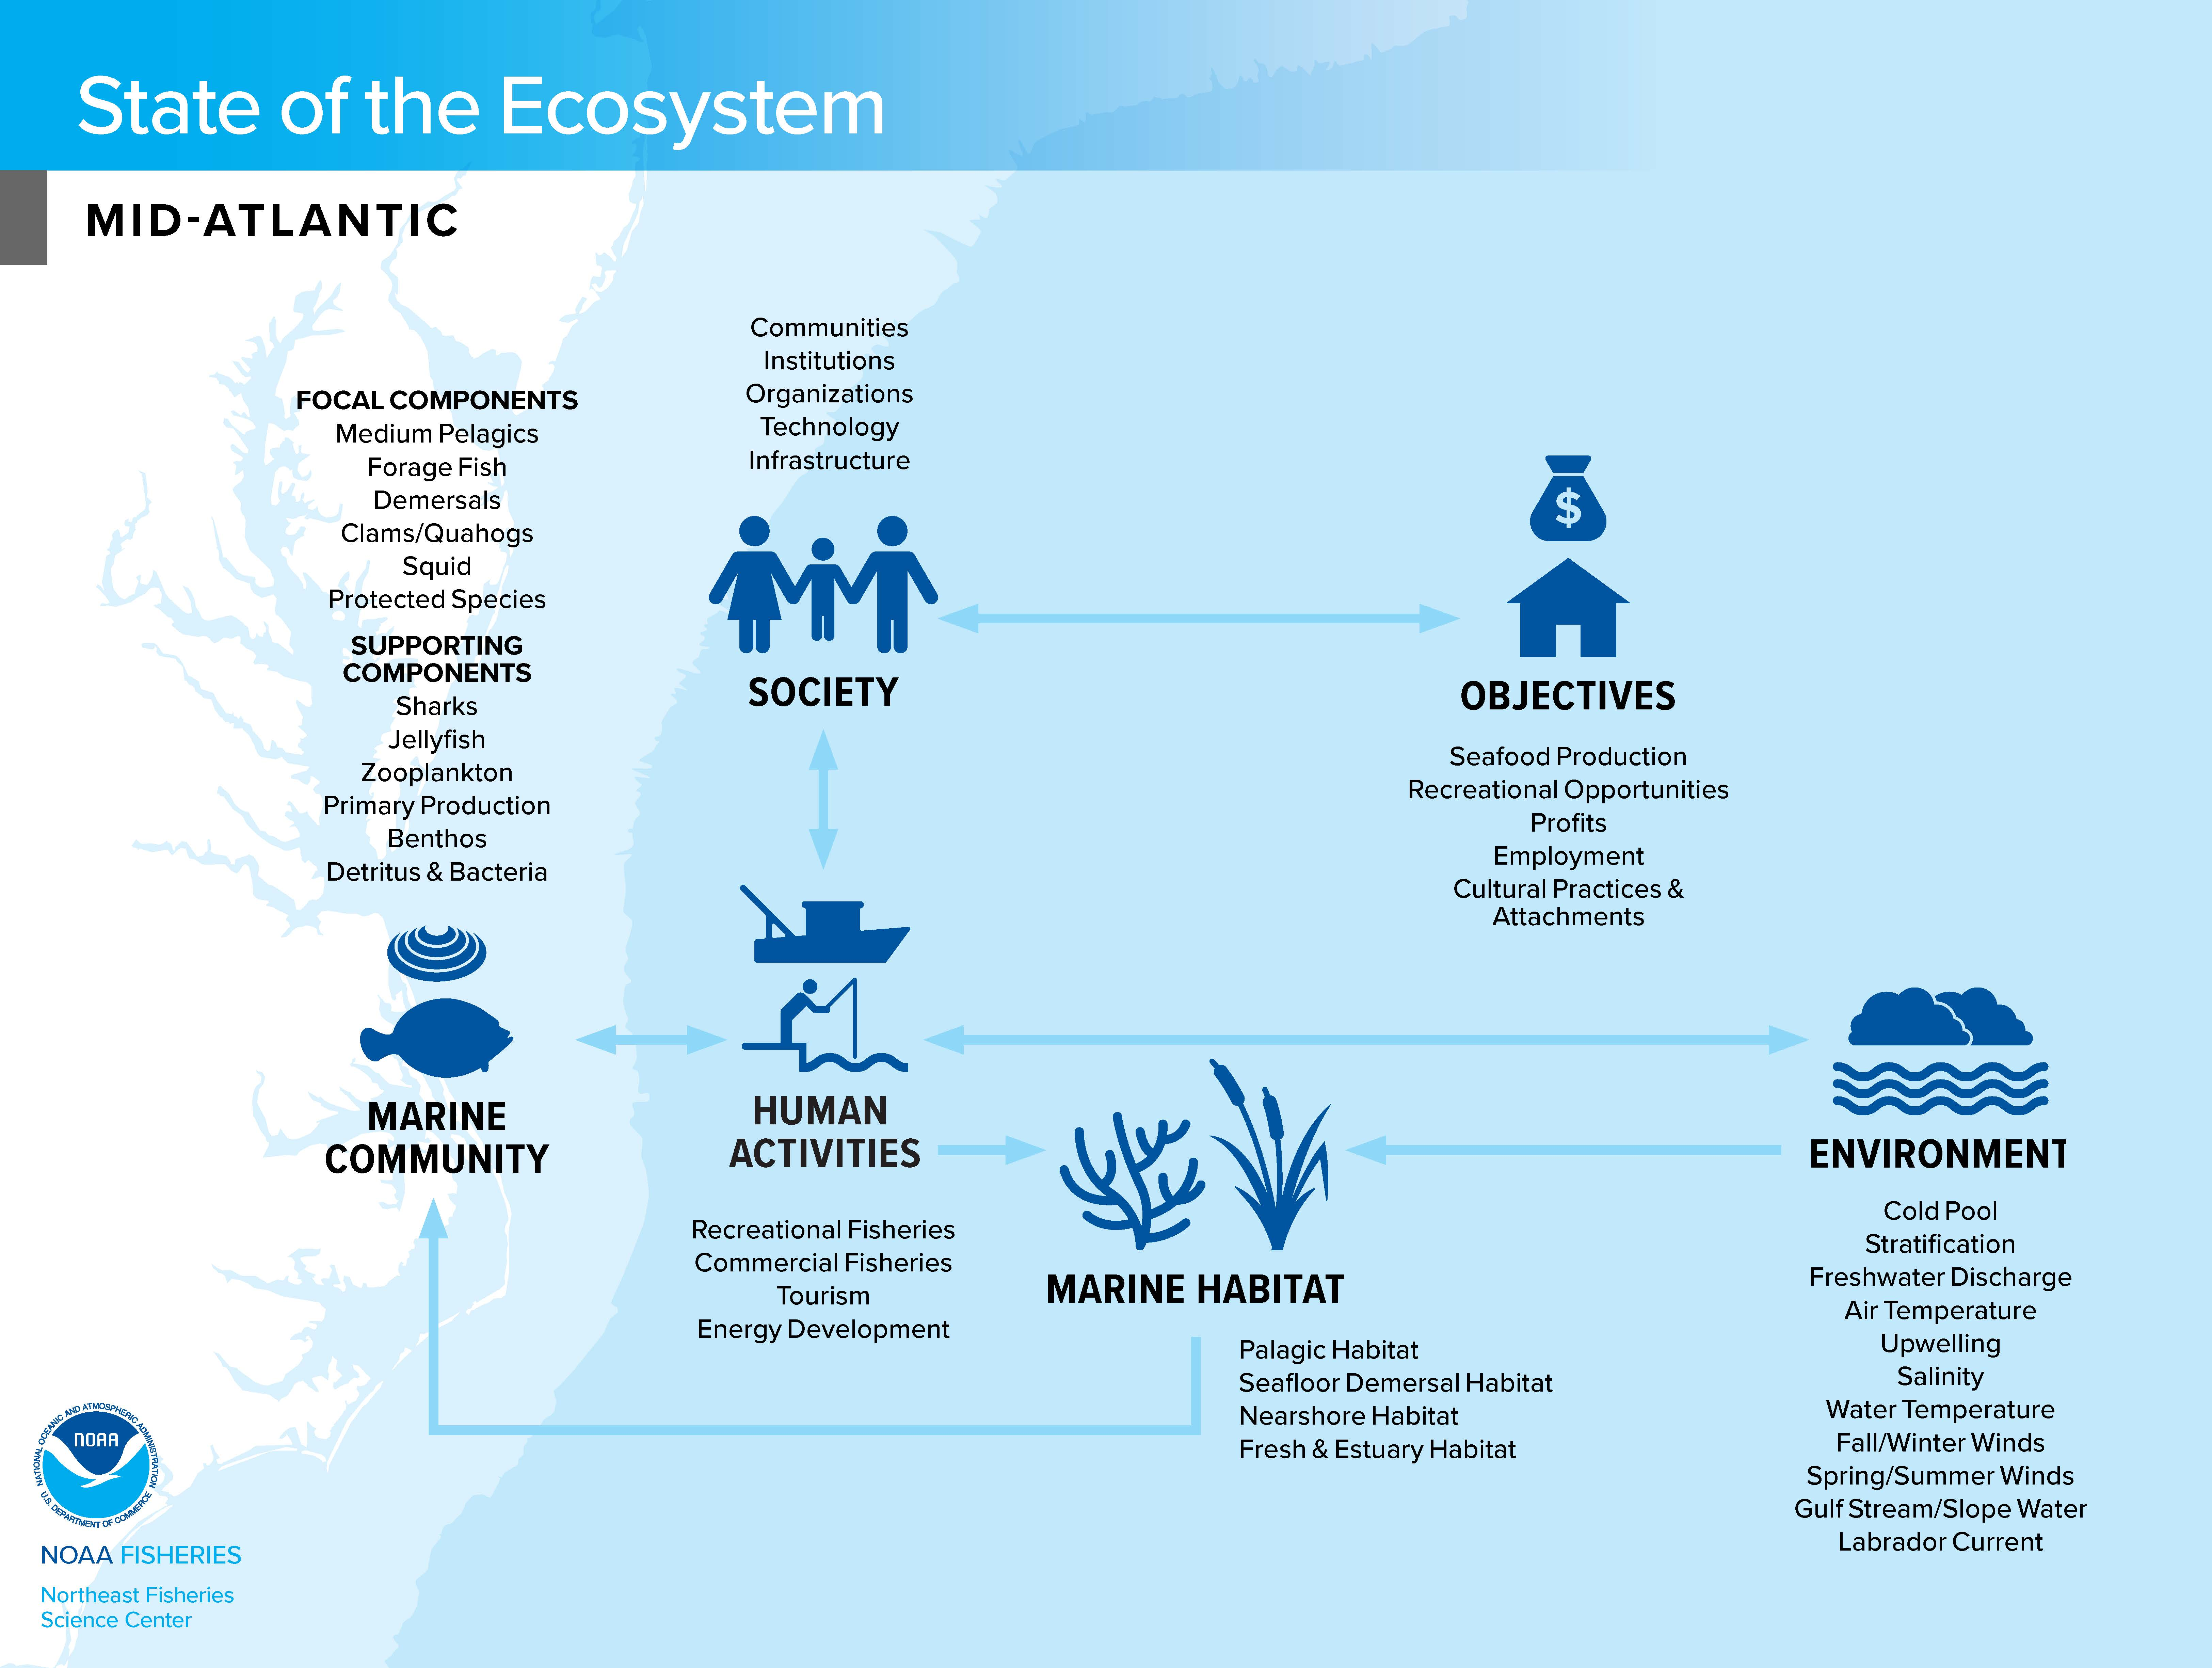
\includegraphics[width=0.8\linewidth]{/home/travis/build/NOAA-EDAB/tech-doc/images/MAB_conmod_overview} \caption{Mid-Atlantic conceptual model for public communication}\label{fig:prettyMA}
\end{figure}

\hypertarget{fish-condition-indicator}{%
\chapter{Fish Condition Indicator}\label{fish-condition-indicator}}

\textbf{Description}: Relative condition

\textbf{Found in}: State of the Ecosystem - Gulf of Maine \& Georges Bank (2018, 2019, 2020), State of the Ecosystem - Mid-Atlantic (2018, 2019, 2020)

\textbf{Indicator category}: Database pull with analysis

\textbf{Contributor(s)}: Laurel Smith

\textbf{Data steward}: Laurel Smith, \href{mailto:laurel.smith@noaa.gov}{\nolinkurl{laurel.smith@noaa.gov}}

\textbf{Point of contact}: Laurel Smith, \href{mailto:laurel.smith@noaa.gov}{\nolinkurl{laurel.smith@noaa.gov}}

\textbf{Public availability statement}: NEFSC survey data used in these analyses are available upon request (see \href{https://inport.nmfs.noaa.gov/inport/item/22560}{BTS metadata} for access procedures). Derived condition data are available \href{https://comet.nefsc.noaa.gov/erddap/tabledap/gf_condition_soe_v1.html}{here}.

\hypertarget{methods-13}{%
\section{Methods}\label{methods-13}}

Relative condition (Kn) was introduced by Cren (\protect\hyperlink{ref-Cren1951a}{1951}) as a way to remove the influence of length on condition, and Blackwell, Brown, and Willis (\protect\hyperlink{ref-Blackwell2000}{2000}) noted that Kn may be useful in detecting prolonged physical stress on a fish populations. Relative condition is calculated as
\[Kn = W/W',\] where \(W\) is the weight of an individual fish and \(W'\) is the predicted length-specific mean weight for the fish population in a given region. Here, relative condition was calculated for finfish stocks commonly caught on the Northeast Fisheries Science Center's (NEFSC) autumn bottom trawl survey, from 1992-present.

Where data allowed, predicted length-weight parameters were calculated for \(W’\) by species, sex and season over the time period 1992-2012. When sample sizes of individual fish weights and lengths were too low, parameters were calculated for aggregated spring and fall survey data over the same time period. Fall survey relative condition was calculated by Ecological Production Unit (EPU) for females only, as trends tended to be similar for males and females.

The \texttt{Condition} package used for calculations and plotting of fish condition factor can be found on \href{https://github.com/Laurels1/Condition}{GitHub}.

\hypertarget{data-sources-13}{%
\subsection{Data sources}\label{data-sources-13}}

Individual fish lengths (to the nearest 0.5 cm) and weights (grams) were collected on the NEFSC bottom trawl surveys from 1992-present aboard RVs Albatross IV, Delaware II and the Henry B. Bigelow (see \protect\hyperlink{survdat}{Survdat}). A small number of outlier values were removed when calculating the length-weight parameters.

\hypertarget{data-extraction-12}{%
\subsection{Data extraction}\label{data-extraction-12}}

Data were extracted from NEFSC's survey database (SVDBS) using the R script found \href{https://github.com/Laurels1/Condition/blob/master/R/pull_from_svdbs.R}{here}

\hypertarget{data-analysis-12}{%
\subsection{Data analysis}\label{data-analysis-12}}

The following growth curve was fit through individual fish lengths and weights from the NEFSC bottom trawl survey data from 1992-2012 to produce reference length-weight parameters:

\[\textrm{Weight} = e^{Fall_{coef}} * \textrm{Length}^{Fall_{exp}},\]

where length is in cm and weight is in kg. Fall survey data were used where sample sizes allowed for growth curve estimation, otherwise data from spring and fall seasons were combined.

Individual fish lengths from the NEFSC fall bottom trawl survey from 1992-2017 were then used to calculate predicted weights using the reference length-weight parameters. Relative condition (\(Kn\)) was calculated annually for females by species and EPU by dividing individual fish weights by the predicted weight.

The code found \href{https://github.com/Laurels1/Condition/blob/master/R/RelConditionEPU.R}{here} was used in the analysis of fish condition.

\hypertarget{plotting-9}{%
\subsection{Plotting}\label{plotting-9}}

Code for plotting the fish condition indicator can be found \href{https://github.com/Laurels1/Condition/blob/master/R/Condition_plot_viridis_final.R}{here}.

\begin{figure}
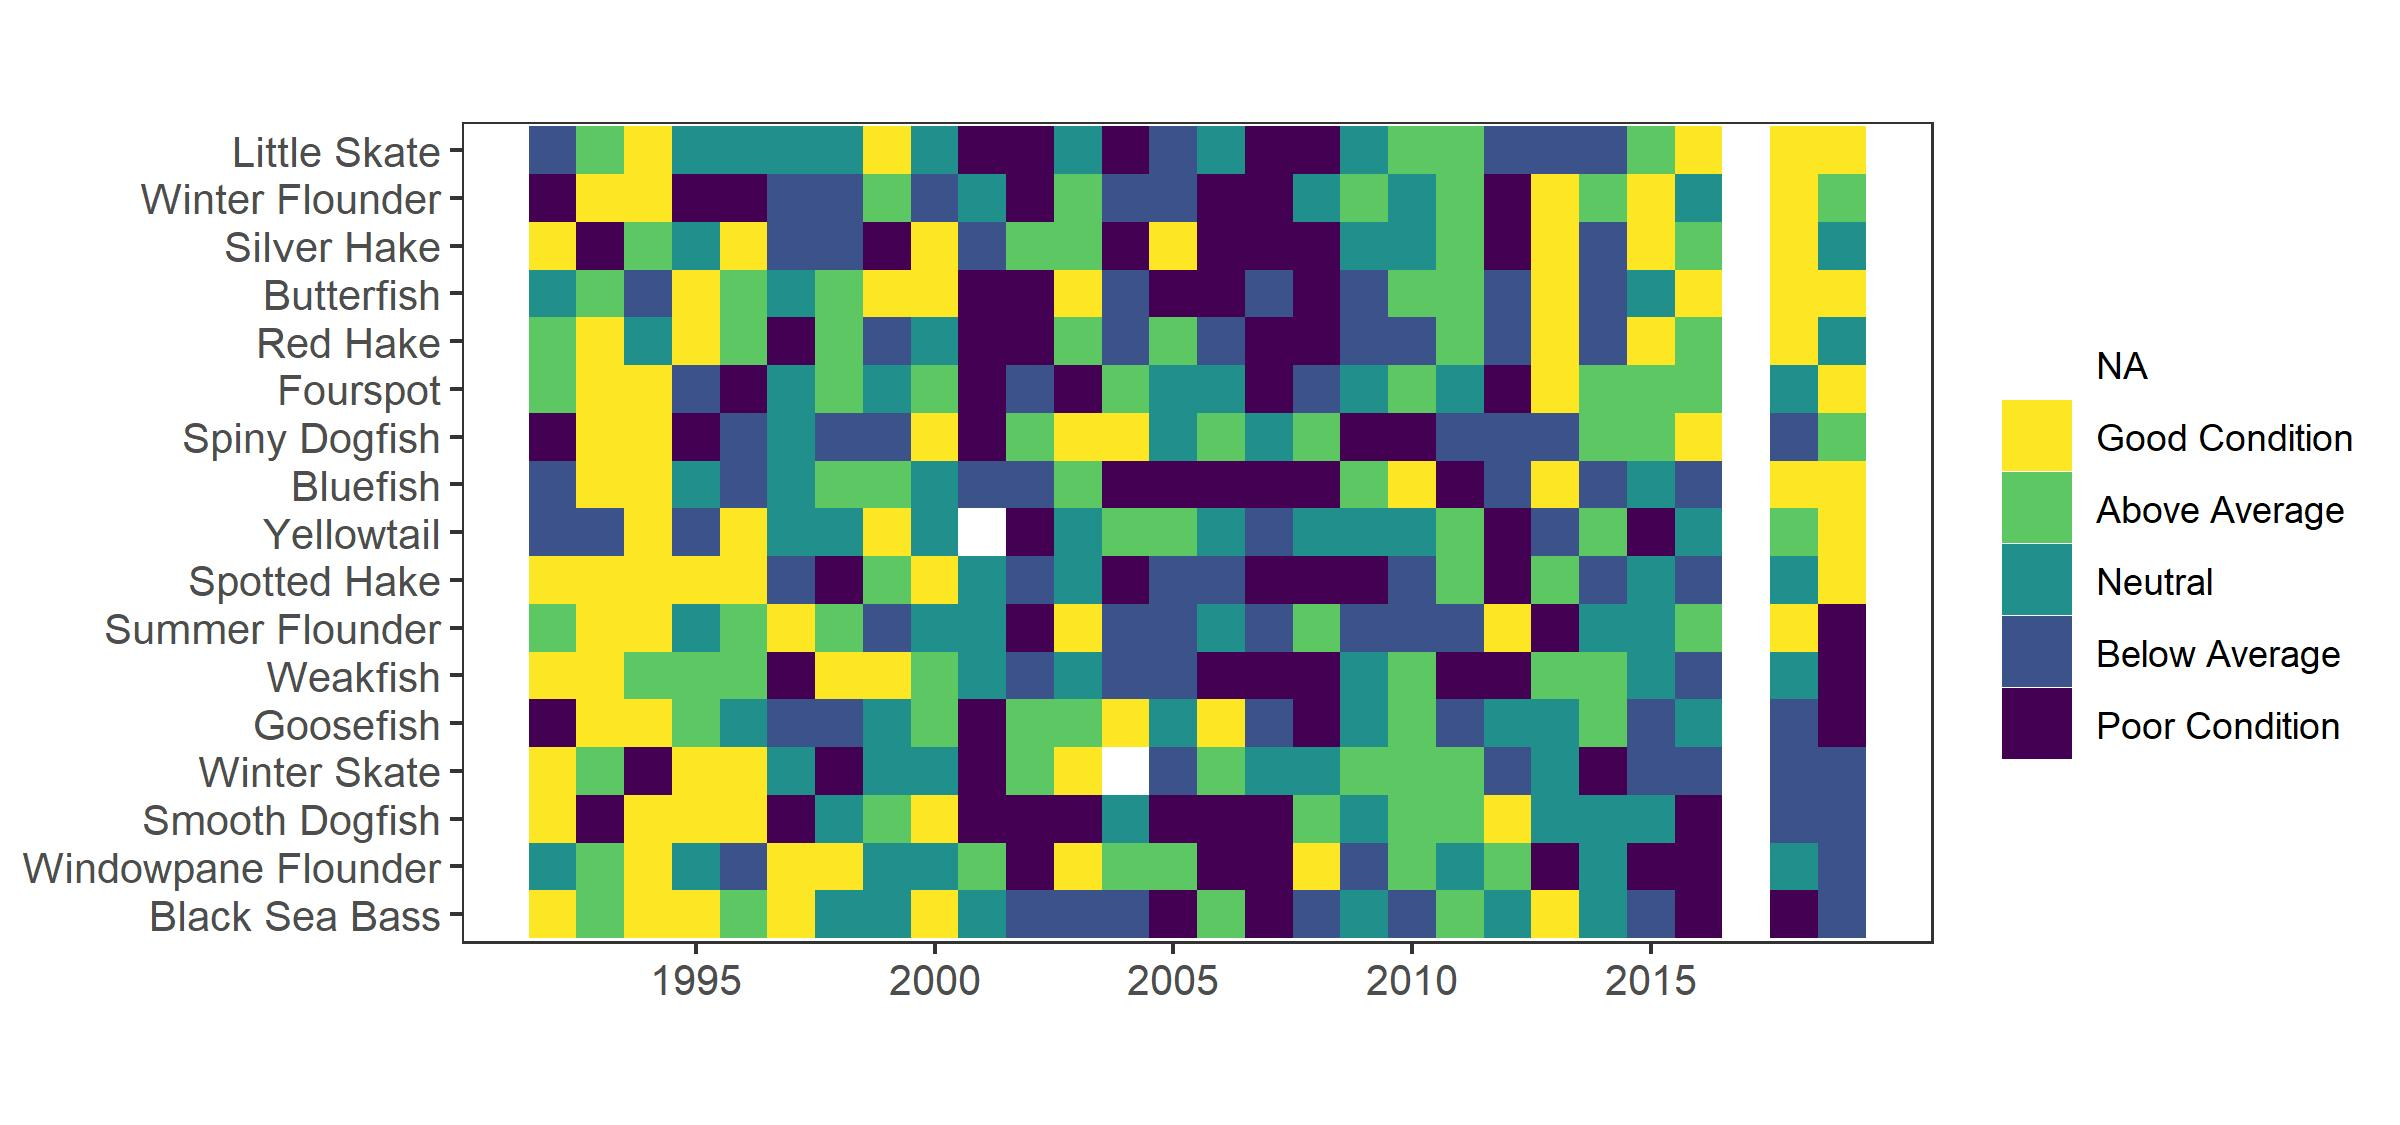
\includegraphics[width=33.33in]{/home/travis/build/NOAA-EDAB/tech-doc/images/MABcondition_2019_viridis_final} \caption{ Condition factor for fish species in the MAB. MAB data are missing for 2017 due to survey delays.}\label{fig:unnamed-chunk-16}
\end{figure}

\hypertarget{epu}{%
\chapter{Ecological Production Units}\label{epu}}

\textbf{Description}: Ecological Production Units

\textbf{Found in}: State of the Ecosystem - Gulf of Maine \& Georges Bank (2018, 2019, 2020), State of the Ecosystem - Mid-Atlantic (2018, 2019, 2020)

\textbf{Indicator category}: Extensive analysis, not yet published

\textbf{Contributor(s)}: Robert Gamble

\textbf{Data steward}: NA

\textbf{Point of contact}: Robert Gamble, \href{mailto:robert.gamble@noaa.gov}{\nolinkurl{robert.gamble@noaa.gov}}

\textbf{Public availability statement}: Ecological production unit (EPU) shapefiles are available \href{https://github.com/NOAA-EDAB/tech-doc/tree/master/gis}{here}. More information about source data used to derive EPUs can be found \href{https://www.integratedecosystemassessment.noaa.gov/sites/default/files/pdf/ne-ecological-production-units-paper.pdf}{here}.

\hypertarget{methods-14}{%
\section{Methods}\label{methods-14}}

To define ecological production units (EPUs), we assembled a set of physiographic, oceanographic and biotic variables on the Northeast U.S. Continental Shelf, an area of approximately 264,000 km within the 200 m isobath. The physiographic and hydrographic variables selected have been extensively used in previous analyses of oceanic provinces and regions (e.g Roff and Taylor \protect\hyperlink{ref-Roff2000}{2000}). Primary production estimates have also been widely employed for this purpose in conjunction with physical variables (Longhurst \protect\hyperlink{ref-Longhurst2007}{2007}) to define ecological provinces throughout the world ocean.

We did not include information on zooplankton, benthic invertebrates, fish, protected species, or fishing patterns in our analysis. The biomass and production of the higher trophic level groups in this region has been sharply perturbed by fishing and other anthropogenic influences. Similarly, fishing patterns are affected by regulatory change, market and economic factors and other external influences.

Because these malleable patterns of change are often unconnected with underlying productivity, we excluded factors directly related to fishing practices. The physiographic variables considered in this analysis are listed in Table \ref{tab:epuinputs}. They include bathymetry and surficial sediments. The physical oceanographic and hydrographic measurements include sea surface temperature, annual temperature span, and temperature gradient water derived from satellite observations for the period 1998 to 2007.

\hypertarget{data-sources-14}{%
\subsection{Data sources}\label{data-sources-14}}

Shipboard observations for surface and bottom water temperature and salinity in surveys conducted in spring and fall. Daily sea surface temperature (SST, °C) measurements at 4 km resolution were derived from nighttime scenes composited from the AVHRR sensor on NOAA's polar-orbiting satellites and from NASA's MODIS TERRA and MODIS AQUA sensors. We extracted information for the annual mean SST, temperature span, and temperature gradients from these sources. The latter metric provides information on frontal zone locations.

\begin{table}

\caption{\label{tab:epuinputs}Variables used in derivation of Ecological Production Units.}
\centering
\begin{tabular}[t]{lll}
\toprule
Variables & Sampling Method & Units\\
\midrule
Surficial Sediments & Benthic Grab & Krumbian Scale\\
Sea Surface Temperature & Satellite Imagery (4km grid) & \&deg;C annual average\\
Sea Surface Temperature & Satellite Imagery (4km grid) & dimensionless\\
Sea Surface Temperature & Satellite Imagery (4km grid) & \&deg;C annual average\\
Surface Temperature & Shipboard hydrography (point) & \&deg;C (Spring and Fall)\\
\addlinespace
Bottom Temperature & Shipboard hydrography (point) & \&deg;C (Spring and Fall)\\
Surface Salinity & Shipboard hydrography (point) & psu (Spring and Fall)\\
Bottom Salinity & Shipboard hydrography (point) & psu (Spring and Fall)\\
Stratification & Shipboard hydrography (point) & Sigma-t units (Spring and Fall)\\
Chlorophyll-a & Satellite Imagery (1.25 km grid) & mg/C/m\textasciicircum{}3\textasciicircum{} (annual average)\\
\addlinespace
Chlorophyll-a gradient & Satellite Imagery (1.25 km grid) & dimensionless\\
Chlorophyll-a span & Satellite Imagery (1.25 km grid) & mg/C/m\textasciicircum{}3\textasciicircum{} (annual average)\\
Primary Production & Satellite Imagery (1.25 km grid) & gC/m\textasciicircum{}3\textasciicircum{}/year (cumulative)\\
Primary Production gradient & Satellite Imagery (1.25 km grid) & dimensionless\\
Primary Production span & Satellite Imagery (1.25 km grid) & gC/m\textasciicircum{}3\textasciicircum{}/year (cumulative)\\
\bottomrule
\end{tabular}
\end{table}

The biotic measurements included satellite-derived estimates of chlorophyll \emph{a} (CHLa) mean concentration, annual span, and CHLa gradients and related measures of primary production. Daily merged SeaWiFS/MODIS-Aqua CHLa (CHL, mg m\textsuperscript{-3}) and SeaiWiFS photosynthetically available radiation (PAR, Einsteins m\textsuperscript{-2} d\textsuperscript{-1}) scenes at 1.25 km resolution were obtained from NASA Ocean Biology Processing Group.

\hypertarget{data-extraction-13}{%
\subsection{Data extraction}\label{data-extraction-13}}

NA

\hypertarget{data-analysis-13}{%
\subsection{Data analysis}\label{data-analysis-13}}

In all cases, we standardized the data to common spatial units by taking annual means of each observation type within spatial units of 10' latitude by 10' longitude to account for the disparate spatial and temporal scales at which these observations are taken. There are over 1000 spatial cells in this analysis. Shipboard sampling used to obtain direct hydrographic measurements is constrained by a minimum sampling depth of 27 m specified on the basis of prescribed safe operating procedures. As a result nearshore waters are not fully represented in our initial specifications of ecological production units.

The size of the spatial units employed further reflects a compromise between retaining spatial detail and minimizing the need for spatial interpolation of some data sets. For shipboard data sets characterized by relatively coarse spatial resolution, where necessary, we first constructed an interpolated map using an inverse distance weighting function before including it in the analysis. Although alternative interpolation schemes based on geostatistical approaches are possible, we considered the inverse distance weighting function to be both tractable and robust for this application.

We first employed a spatial principal components analysis (PCA; e.g.~Pielou \protect\hyperlink{ref-Pielou1984}{1984}; Legendre and Legendre \protect\hyperlink{ref-Legendre1998}{1998}) to examine the multivariate structure of the data and to account for any inter-correlations among the variables to be used in subsequent analysis. The variables included in the analysis exhibited generally skewed distributions and we therefore transformed each to natural logarithms prior to analysis.

The PCA was performed on the correlation matrix of the transformed observations. We selected the eigenvectors associated with eigenvalues of the dispersion matrix with scores greater than 1.0 (the Kaiser-Guttman criterion; Legendre and Legendre \protect\hyperlink{ref-Legendre1998}{1998}) for all subsequent analysis. These eigenvectors represent orthogonal linear combinations of the original variables used in the analysis.

We delineated ecological subunits by applying a disjoint cluster based on Euclidean distances using the K-means procedure (Legendre and Legendre \protect\hyperlink{ref-Legendre1998}{1998}) on the principal component scores The use of non-independent variables can strongly influence the results of classification analyses of this type (Pielou \protect\hyperlink{ref-Pielou1984}{1984}), hence the interest in using the PCA results in the cluster.

The eigenvectors were represented as standard normal deviates. We used a Pseudo-F Statistic described by Milligan and Cooper (\protect\hyperlink{ref-Milligan1985}{1985}) to objectively define the number of clusters to use in the analysis. The general approach employed is similar to that of Host et al. (\protect\hyperlink{ref-Host1996}{1996}) for the development of regional ecosystem classifications for terrestrial systems.

After the analyses were done, we next considered options for interpolation of nearshore boundaries resulting from depth-related constraints on shipboard observations. For this, we relied on information from satellite imagery. For the missing nearshore areas in the Gulf of Maine and Mid-Atlantic Bight, the satellite information for chlorophyll concentration and sea surface temperature indicated a direct extension from adjacent observations. For the Nantucket Shoals region south of Cape Cod, similarities in tidal mixing patterns reflected in chlorophyll and temperature observations indicated an affinity with Georges Bank and the boundaries were changed accordingly.

Finally, we next considered consolidation of ecological subareas so that nearshore regions are considered to be special zones nested within the adjacent shelf regions. Similar consideration led to nesting the continental slope regions within adjacent shelf regions in the Mid-Atlantic and Georges Bank regions. This led to four major units: Mid-Atlantic Bight, Georges Bank, Western-Central Gulf of Maine (simply ``Gulf of Maine'' in the State of the Ecosystem), and Scotian Shelf-Eastern Gulf of Maine. As the State of the Ecosystem reports are specific to FMC managed regions, the Scotian Shelf-Eastern Gulf of Maine EPU is not considered in SOE indicator analyses.

\begin{figure}

{\centering 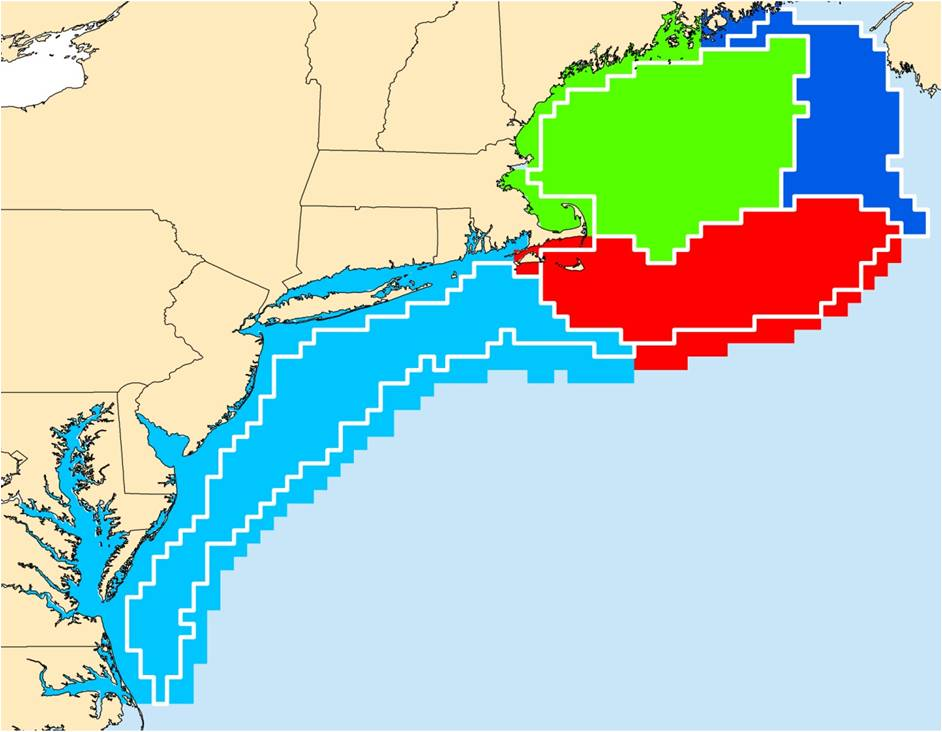
\includegraphics[width=13.08in]{/home/travis/build/NOAA-EDAB/tech-doc/images/EPUs} 

}

\caption{Map of the four Ecological Production Units, including the Mid-Atlantic Bight (light blue), Georges Bank (red), Western-Central Gulf of Maine (or Gulf of Maine; green), and Scotian Shelf-Eastern Gulf of Maine (dark blue)}\label{fig:EPUmap}
\end{figure}

\hypertarget{data-processing-10}{%
\subsection{Data processing}\label{data-processing-10}}

Shapefiles were converted to \texttt{sf} objects for inclusion in the \texttt{ecodata} R package using the R code found \href{https://raw.githubusercontent.com/NOAA-EDAB/ecodata/master/data-raw/get_epu_sf.R}{here}.

\hypertarget{forage-fish-energy-density}{%
\chapter{Forage Fish Energy Density}\label{forage-fish-energy-density}}

\textbf{Description}: Forage Engery Density indicators

\textbf{Found in}: State of the Ecosystem - Gulf of Maine \& Georges Bank (2020), State of the Ecosystem - Mid-Atlantic (2020)

\textbf{Indicator category}: Database pull with analysis

\textbf{Contributor(s)}: Mark Wuenschel, Ken Oliveira and Kelcie Bean

\textbf{Data steward}: Mark Wuenschel \href{mailto:mark.wuenschel@noaa.gov}{\nolinkurl{mark.wuenschel@noaa.gov}}

\textbf{Point of contact}: Mark Wuenschel \href{mailto:mark.wuenschel@noaa.gov}{\nolinkurl{mark.wuenschel@noaa.gov}}

\textbf{Public availability statement}: Source data are publicly available.

\hypertarget{methods-15}{%
\section{Methods}\label{methods-15}}

The forage fish energy denisty indicator comes from a collaborative project between UMASS Dartmouth Biology Department (Dr.~Ken Oliveira, M.S student Kelcie Bean) and NEFSC Population Biology Branch (Mark Wuenschel). The study focuses on evaluating energy content of the species in Table \ref{tab:foragefish}.

\begin{table}

\caption{\label{tab:foragefish}List of forage fish study species.}
\centering
\begin{tabular}[t]{ll}
\toprule
Common Name & Scientific Name\\
\midrule
Atlantic Herring & *Clupea harengus*\\
alewife & *Alosa pseudoharengus*\\
silver hake & *Merluccius bilinearis*\\
butterfish & *Peprilus triacanthus*\\
northern sandlance & *Ammodytes dubius*\\
\addlinespace
Atlantic mackerel & *Scomber Scombrus*\\
longfin squid & *Loligo pealeii*\\
northern shortfin squid & *Illex illecebrosus*\\
\bottomrule
\end{tabular}
\end{table}

\hypertarget{data-sources-15}{%
\subsection{Data sources}\label{data-sources-15}}

2017 and 2018 NEFSC spring and fall bottom trawl surveys.

\hypertarget{data-extraction-14}{%
\subsection{Data extraction}\label{data-extraction-14}}

NA

\hypertarget{data-analysis-14}{%
\subsection{Data analysis}\label{data-analysis-14}}

Samples were analyzed for proximate composition and energy density from 2017 and 2018 NEFSC spring and fall bottom trawl surveys. Predictive relationships between the percent dry weight of samples and energy density were developed, and samples collected from 2019 surveys are currently being analyzed for percentage dry weight to enable estimation of energy content (Bean (\protect\hyperlink{ref-Bean2020}{2020})). The energy density of forage species differed from prior studies in the 1980s and 1990s (Steimle and Terranova (\protect\hyperlink{ref-steimle1985}{1985}), Lawson, Magalhães, and Miller (\protect\hyperlink{ref-lawson1998}{1998}), Table \ref{tab:tab}).

Sampling and laboratory analysis is ongoing, with the goal of continuing routine monitoring of energy density of these species.

\hypertarget{data-processing-11}{%
\subsection{Data processing}\label{data-processing-11}}

Code for building the table used in the SOE can be found
\href{https://github.com/NOAA-EDAB/ecodata/blob/master/chunk-scripts/macrofauna.Rmd-forage.R}{here}.

\begin{table}

\caption{\label{tab:tab}Forage fish energy content}
\centering
\fontsize{9}{11}\selectfont
\begin{tabular}[t]{l|l|r|l|r|l|r|l|r|l|r|r|l}
\hline
\multicolumn{1}{c|}{ } & \multicolumn{4}{c|}{2017} & \multicolumn{4}{c|}{2018} & \multicolumn{2}{c|}{Total} & \multicolumn{1}{c|}{Steimle and Terranove (1985)} & \multicolumn{1}{c}{Lawson et al. (1998)} \\
\cline{2-5} \cline{6-9} \cline{10-11} \cline{12-12} \cline{13-13}
\multicolumn{1}{c|}{ } & \multicolumn{2}{c|}{Spring} & \multicolumn{2}{c|}{Fall} & \multicolumn{2}{c|}{Spring} & \multicolumn{2}{c|}{Fall} & \multicolumn{4}{c}{ } \\
\cline{2-3} \cline{4-5} \cline{6-7} \cline{8-9}
Species & Mean ED (SD) & N & Mean ED (SD) & N & Mean ED (SD) & N & Mean ED (SD) & N & Mean ED (SD) & N & Mean ED & Mean ED (SD)\\
\hline
Alewife & 6.84 (1.62) & 128 & 8.12 (1.46) & 50 & 6.45 (1.21) & 47 & 7.41 (1.6) & 42 & 7.1 (1.62) & 267 & 6.4 & \\
\hline
Atl. Herring & 5.34 (0.94) & 122 & 5.77 (1.31) & 52 & 6.69 (0.85) & 51 & 5.41 (1.34) & 50 & 5.69 (1.19) & 275 & 10.6 & 9.4 (1.4)\\
\hline
Atl. Mackerel &  & NA & 7.24 (1.13) & 50 & 5.33 (0.86) & 51 & 6.89 (1.07) & 50 & 6.48 (1.32) & 151 & 6.0 & \\
\hline
Butterfish & 7.13 (1.59) & 65 & 7.31 (1.45) & 89 & 4.91 (1.12) & 53 & 8.1 (2.7) & 50 & 6.92 (2.04) & 257 & 6.2 & \\
\hline
Illex & 5.54 (0.4) & 77 & 5.43 (0.51) & 52 & 5.5 (0.52) & 50 & 4.76 (0.79) & 50 & 5.33 (0.63) & 229 & 7.1 & 5.9 (0.56)\\
\hline
Loligo & 5.22 (0.36) & 83 & 5.24 (0.26) & 60 & 4.84 (0.63) & 52 & 4.6 (0.72) & 50 & 5.02 (0.56) & 245 & 5.6 & \\
\hline
Sand lance & 6.66 (0.54) & 18 &  & NA & 5.78 (0.34) & 60 & 7.99 (0.74) & 8 & 6.17 (0.81) & 86 & 6.8 & 4.4 (0.82)\\
\hline
Silver hake & 4.25 (0.39) & 189 & 4.42 (0.45) & 50 & 4.19 (0.39) & 50 & 4.55 (0.63) & 50 & 4.31 (0.46) & 339 & 4.6 & \\
\hline
\end{tabular}
\end{table}

\hypertarget{gulf-stream-index}{%
\chapter{Gulf Stream Index}\label{gulf-stream-index}}

\textbf{Description}: Annual time series of the Gulf Stream index

\textbf{Indicator category}: Published method

\textbf{Found in}: State of the Ecosystem - New England (2019 (Different Methods), 2020),
State of the Ecosystem - Mid-Atlantic (2019 (Different Methods), 2020)

\textbf{Contributor(s)}: Zhuomin Chen, Young-oh Kwon

\textbf{Data steward}: Vincent Saba, \href{mailto:vincent.saba@noaa.gov}{\nolinkurl{vincent.saba@noaa.gov}}

\textbf{Point of contact}: Vincent Saba, \href{mailto:vincent.saba@noaa.gov}{\nolinkurl{vincent.saba@noaa.gov}}

\textbf{Public availability statement}: Source data are publicly available at \href{http://marine.copernicus.eu/services-portfolio/access-to-products/?option=com_csw\&view=details\&product_id=SEALEVEL_GLO_PHY_L4_REP_OBSERVATIONS_008_047}{CMENS}. Index data are NOT publically available so please email \href{mailto:vincent.saba@noaa.gov}{\nolinkurl{vincent.saba@noaa.gov}} for further information and queries of GSI indicator data.

\hypertarget{methods-16}{%
\section{Methods}\label{methods-16}}

The methods used to calculate the Gulf Stream Index changed between 2019 and 2020 SOEs. The most recent methods and at the top with older methods below those.

\hypertarget{data-sources-16}{%
\subsection{Data sources}\label{data-sources-16}}

GLOBAL OCEAN GRIDDED L4 SEA SURFACE HEIGHTS AND DERIVED VARIABLES REPROCESSED (1993-ONGOING). \url{http://marine.copernicus.eu/services-portfolio/access-to-products/?option=com_csw\&view=details\&product_id=SEALEVEL_GLO_PHY_L4_REP_OBSERVATIONS_008_047}

\hypertarget{data-analysis-15}{%
\subsection{Data analysis}\label{data-analysis-15}}

The GSI is calculated based on the method presented by Pérez-Hernández and Joyce (\protect\hyperlink{ref-perez-hernandez2014}{2014}). It is a simple 16-point GS index constructed by selecting grid points following the maximum Standard deviation of sea level height anomalies every 1.33° longitude between 52° and 72°W and averaging them. The value of 1.33° is based on the resolution of satellite dataset from AVISO. We followed the same method, except using the dataset from \href{http://marine.copernicus.eu/services-portfolio/access-to-products/?option=com_csw\&view=details\&product_id=SEALEVEL_GLO_PHY_L4_REP_OBSERVATIONS_008_047}{CMEMS}, which has a 0.25°x0.25° resolution. Therefore we select points every 1° between 52° and 72° and average them, and there are 21 points in total.

\hypertarget{data-processing-12}{%
\subsection{Data Processing}\label{data-processing-12}}

The Gulf Stream index data set was formatted for inclusion in the \texttt{ecodata} R package with the code found \href{https://github.com/NOAA-EDAB/ecodata/blob/master/data-raw/get_gsi.R}{here}.

\hypertarget{plotting-10}{%
\subsection{Plotting}\label{plotting-10}}

The plot below was built using the code found
\href{https://github.com/NOAA-EDAB/ecodata/blob/master/chunk-scripts/LTL.Rmd-GSI.R}{here}.

\begin{figure}
\centering
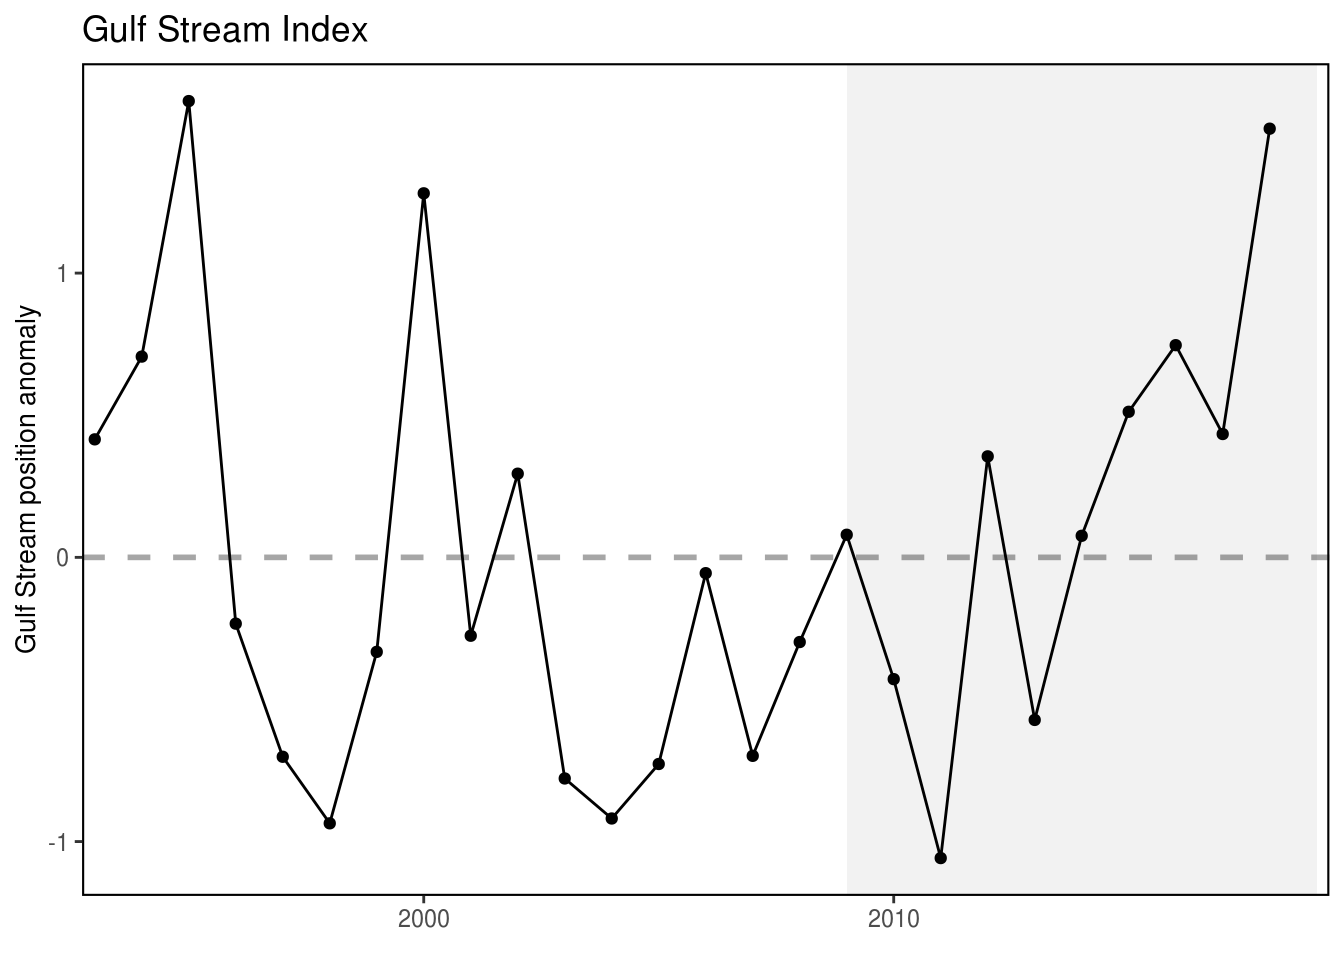
\includegraphics{/home/travis/build/NOAA-EDAB/tech-doc/images/unnamed-chunk-17-1.pdf}
\caption{\label{fig:unnamed-chunk-17}Gulf Stream Index}
\end{figure}

\hypertarget{methods-17}{%
\section{2019 Methods}\label{methods-17}}

Summarized from Joyce et al. (\protect\hyperlink{ref-joyce2019}{2019}), ocean temperature data from NOAA NODC were sorted by latitude, longitude, and time using a resolution of 1\textdegree of longitude, latitude, and 3 months of time, respectively, with a Gaussian squared weighting from the selected desired point in a window twice the size of the desired resolution. Editing was used to reject duplicate samples and 3\(\sigma\) outliers from each selected sample point prior to performing the weighting and averaging; the latter was only carried out when there were at least three data points in the selected interval for each sample point. Typically, 50 or more data values were available. The resulting temperature field was therefore smoothed. Data along the Gulf Stream north wall at nine data points were used to assemble a spatial/temporal sampling of the temperature at 200m data along the north wall from 75\textdegree W to 55\textdegree W. The leading mode of temperature variability of the Gulf Stream is equivalent to a north‐south shift of 50--100 km, which is zonally of one sign and amounts to 50\% of the seasonal‐interannual variance between 75\textdegree W and 55\textdegree W. The temporal behavior of this mode (PC1) shows the temporal shift of the Gulf Stream path with a dominant approximately 8‐ to 10‐year periodicity over much of the period.

\hypertarget{data-sources-17}{%
\subsection{Data Sources}\label{data-sources-17}}

Ocean temperatures at 200 m are available at \url{https://www.nodc.noaa.gov/OC5/3M_HEAT_CONTENT/}.

\hypertarget{data-analysis-16}{%
\subsection{Data analysis}\label{data-analysis-16}}

For detailed analytical methods, see Joyce et al. (\protect\hyperlink{ref-joyce2019}{2019}).

\hypertarget{data-processing-and-plotting}{%
\subsection{Data processing and plotting}\label{data-processing-and-plotting}}

Data processing and plotting remained the same between years.

\hypertarget{harbor-porpoise-bycatch}{%
\chapter{Harbor Porpoise Bycatch}\label{harbor-porpoise-bycatch}}

\textbf{Description}: Harbor Porpoise Indicator

\textbf{Found in}: State of the Ecosystem - Gulf of Maine \& Georges Bank (2018, 2019), State of the Ecosystem - Mid-Atlantic (2018, 2019)

\textbf{Indicator category}: Synthesis of published information; Published methods

\textbf{Contributor(s)}: Christopher D. Orphandies

\textbf{Data steward}: Chris Orphanides, \href{mailto:chris.orphanides@noaa.gov}{\nolinkurl{chris.orphanides@noaa.gov}}

\textbf{Point of contact}: Chris Orphanides, \href{mailto:chris.orphanides@noaa.gov}{\nolinkurl{chris.orphanides@noaa.gov}}

\textbf{Public availability statement}: Source data are available in public \href{https://www.fisheries.noaa.gov/national/marine-mammal-protection/marine-mammal-stock-assessment-reports-region}{stock assessment reports} (2018 report in-press). Derived data as shown in the 2018 SOE reports are available \href{http://comet.nefsc.noaa.gov/erddap/tabledap/protected_species_soe_v1.html}{here}

\hypertarget{methods-18}{%
\section{Methods}\label{methods-18}}

\hypertarget{data-sources-18}{%
\subsection{Data sources}\label{data-sources-18}}

Reported harbor porpoise bycatch estimates and potential biological removal levels can be found in publicly available documents; detailed \href{https://www.fisheries.noaa.gov/national/marine-mammal-protection/marine-mammal-stock-assessment-reports-region}{here}. The most recent bycatch estimates for 2016 were taken from the 2018 stock assessment (in-press). More detailed documentation as to the methods employed can be found in NOAA Fisheries Northeast Fisheries Science Center (NEFSC) Center Reference Documents (CRDs) found on the NEFSC \href{https://www.nefsc.noaa.gov/publications/crd/}{publications page}.

The document for the 2016 estimates (CRD 19-04) is available \href{https://www.nefsc.noaa.gov/publications/crd/crd1904/crd1904.pdf}{here}. Additional methodological details are available for previous year's estimates and are documented in numerous published CRDs: \href{https://www.nefsc.noaa.gov/publications/crd/crd1718/crd1718.pdf}{CRD 17-18}, \href{https://www.nefsc.noaa.gov/publications/crd/crd1605/crd1605.pdf}{CRD-16-05}, \href{https://www.nefsc.noaa.gov/publications/crd/crd1515/crd1515.pdf}{CRD 15-15}, \href{https://repository.library.noaa.gov/view/noaa/4718}{CRD 14-02}, \href{https://www.nefsc.noaa.gov/publications/crd/crd1313/crd1313_2nd_ed.pdf}{CRD 13-13}, \href{https://www.nefsc.noaa.gov/publications/crd/crd1108/1108.pdf}{CRD 11-08}, \href{https://www.nefsc.noaa.gov/publications/crd/crd1010/crd1010.pdf}{CRD 10-10}, \href{https://www.nefsc.noaa.gov/publications/crd/crd0720/crd0720.pdf}{CRD 07-20}, \href{https://www.nefsc.noaa.gov/publications/crd/crd0613/crd0613.pdf}{CRD 06-13}, \href{https://www.nefsc.noaa.gov/publications/crd/crd0318/crd0318.pdf}{CRD 03-18}, \href{https://www.nefsc.noaa.gov/publications/crd/crd0115/0115.pdf}{CRD 01-15}, and \href{https://www.nefsc.noaa.gov/publications/crd/pdfs/crd9917.pdf}{CRD 99-17}.

\hypertarget{data-extraction-15}{%
\subsection{Data extraction}\label{data-extraction-15}}

Annual gillnet bycatch estimates are documented in a CRD (see sources above). These feed into the Stock Assessment Reports which report both the annual bycatch estimate and the mean 5-year estimate. The 5-year estimate is the one used for management purposes, so that is the one provided for the SOE plot.

\hypertarget{data-analysis-17}{%
\subsection{Data analysis}\label{data-analysis-17}}

Bycatch estimates as found in stock assessment reports were plotted along with confidence intervals. The confidence intervals were calculated from published CVs assuming a normal distribution (\(\sigma = \mu CV\); \(CI = \bar{x} \pm \sigma * 1.96\)).

Data were analyzed and formatted for inclusion in the \texttt{ecodata} R package using the R code found \href{https://raw.githubusercontent.com/NOAA-EDAB/ecodata/master/data-raw/get_harborporpoise.R}{here}.

\hypertarget{plotting-11}{%
\subsection{Plotting}\label{plotting-11}}

Code used to plot harbor porpoise data can be found \href{https://github.com/NOAA-EDAB/tech-doc/tree/master/R/stored_scripts/hp_indicator_plotting.R}{here}.

\hypertarget{highly-migratory-species-landings}{%
\chapter{Highly Migratory Species Landings}\label{highly-migratory-species-landings}}

\textbf{Description}: Atlantic Highly Migratory Species Landings

\textbf{Found in}: State of the Ecosystem - Gulf of Maine \& Georges Bank (2020), State of the Ecosystem - Mid-Atlantic (2020)

\textbf{Indicator category}: Synthesis of published information, Database pull with analysis

\textbf{Contributor(s)}: George Silva \href{mailto:george.silva@noaa.gov}{\nolinkurl{george.silva@noaa.gov}}, Heather Baertlein \href{mailto:heather.baertlien@noaa.gov}{\nolinkurl{heather.baertlien@noaa.gov}}, and Cliff Hutt \href{mailto:cliff.hutt@noaa.gov}{\nolinkurl{cliff.hutt@noaa.gov}}

\textbf{Data steward}: Kimberly Bastille

\textbf{Point of contact}: Carrie Soltanoff \href{mailto:carrie.solatnoff@noaa.gov}{\nolinkurl{carrie.solatnoff@noaa.gov}}

\textbf{Public availability statement}: The data provided is publicly available via the \href{https://www.fisheries.noaa.gov/national/sustainable-fisheries/commercial-fisheries-landings}{Fisheries of the United States landings portal}.

\hypertarget{methods-19}{%
\section{Methods}\label{methods-19}}

\hypertarget{data-sources-19}{%
\subsection{Data sources}\label{data-sources-19}}

Data from eDealer database (\url{https://www.fisheries.noaa.gov/atlantic-highly-migratory-species/atlantic-highly-migratory-species-dealer-reporting}) and Bluefin Tuna Dealer reports on \href{https://www.accsp.org/what-we-do/safis/}{SAFIS}. The eDealer data were supplemented with GulfFIN records and vessel logbook catches for which no dealer reports were submitted.

\hypertarget{data-extraction-16}{%
\subsection{Data extraction}\label{data-extraction-16}}

Data were processed for Fisheries of the United States and then aggregated by regions to avoid confidentiality issues.

Data of Atlantic shark, swordfish, bigeye tuna, albacore tuna, yellowfin tuna and skipjack tuna were initially extracted from our eDealer database. Additional landings of these HMS not in eDealer were found in GulfFIN records. Bluefin tuna landings data from the Bluefin Tuna Dealer reports in SAFIS were also extracted and combined with the eDealer data for other HMS .

Procedures of quality assurance were conducted. Duplicate records were removed from the data. This may occur from multiple submissions of reports by the same dealer. It may also occur when two or more dealers report the same landings in ``Packing'' situations. While most vessels immediately sell their catch to the dealer at their port of landing, some vessels sell their catch to a dealer(s) in another location. Transport to alternate locations requires processing of the fish to preserve quality. This processing activity is done by the dealer at the port of landing and is referred to as ``Packing''. Differences in federal and state definitions of who is considered the ``dealer'' of the product, and thus ultimately responsible for submitting the landings report, often results in multiple reports being created for the same landings. These duplicate reports need to be accounted for when summarizing the data to reflect accurate landings. Therefore, searches for duplicate reports of the same landing were conducted and eliminated prior to summarizing the data for the Fisheries of the United States.

Revenue from sales to the aquarium trade were also excluded to avoid extreme values associated with shipping live specimens.

All reported landings were converted to live weights using conversion ratios appropriate for the species/species group and reported grade of the product. Shark fins were not reported to live weight as these weights are included in the converted whole weight of the reported shark landing.

Price per pound was used to determine the ex-vessel value. For landings with prices per pound reported as ``N/A'', 0, \$0.01 or left blank, average prices were calculated for each species and state. Those averages replaced the missing values to determine landings revenue.

The extract only includes species with more than \$1,000 in landings in the region for that year to avoid issues with data confidentiality. Other species landed include: tiger sharks, porbeagle, bonnethead, blacknose, blue, lemon, silky and smooth hammerhead sharks. However, these are not reported because of low volume and resulting data confidentiality issues.

\hypertarget{data-analysis-18}{%
\subsection{Data analysis}\label{data-analysis-18}}

High migratory landings include 19 species of tunas, sharks and swordfish (table @(tab:hms-spp)).

\begin{table}

\caption{\label{tab:hms-spp}Species included in the highly migratory species landings reported in the SOE.}
\centering
\begin{tabular}[t]{l|>{\em}l}
\hline
Common.Name & Scientific.Name\\
\hline
Bluefin Tuna & Thunnus thynnus\\
\hline
Swordfish & Xiphias gladius\\
\hline
Bigeye Tuna & Thunnus obesus\\
\hline
Yellowfin Tuna & Thunnus albacares\\
\hline
Shortfin Mako Shark & Isurus oxyrinchus\\
\hline
Albacore Tuna & Thunnus alalunga\\
\hline
Smooth Dogfish Shark & Mustelus canis\\
\hline
Atlantic Sharpnose Shark & Rhizoprionodon terraenovae\\
\hline
Thresher Shark & Alopias vulpinus\\
\hline
Blacktip Shark & Carcharhinus limbatus\\
\hline
Spinner Shark & Carcharhinus brevipinna\\
\hline
Sandbar Shark & Carcharhinus plumbeus\\
\hline
Great Hammerhead Shark & Sphyrna mokarran\\
\hline
Finetooth Shark & Aprionodon isodon\\
\hline
Skipjack Tuna & Katsuwonus pelamis\\
\hline
Bull Shark & Carcharhinus leucas\\
\hline
Tiger Shark & Galeocerdo cuvier\\
\hline
Scalloped Hammerhead Shark & Sphyrna lewini\\
\hline
Shark fins & NA\\
\hline
\end{tabular}
\end{table}

Data were processed and analyzed using SAS and Microsoft Excel pivot tables. The count of records marked as confidential and the number of states represented in each regional species sum was used to determine if a sufficient number of records were available to make the data public or if it needed to be marked as confidential.

\hypertarget{data-processing-13}{%
\subsection{Data processing}\label{data-processing-13}}

HMS landings data were formatted for inclusion in the \texttt{ecodata} R package using the R code found \href{https://github.com/NOAA-EDAB/ecodata/blob/master/data-raw/get_hms_landings.R}{here}.

\hypertarget{plotting-12}{%
\subsection{Plotting}\label{plotting-12}}

The plot below was built using the code found
\href{https://github.com/NOAA-EDAB/ecodata/blob/master/chunk-scripts/human_dimensions.Rmd-comm_landings.R}{here}.

\begin{figure}
\centering
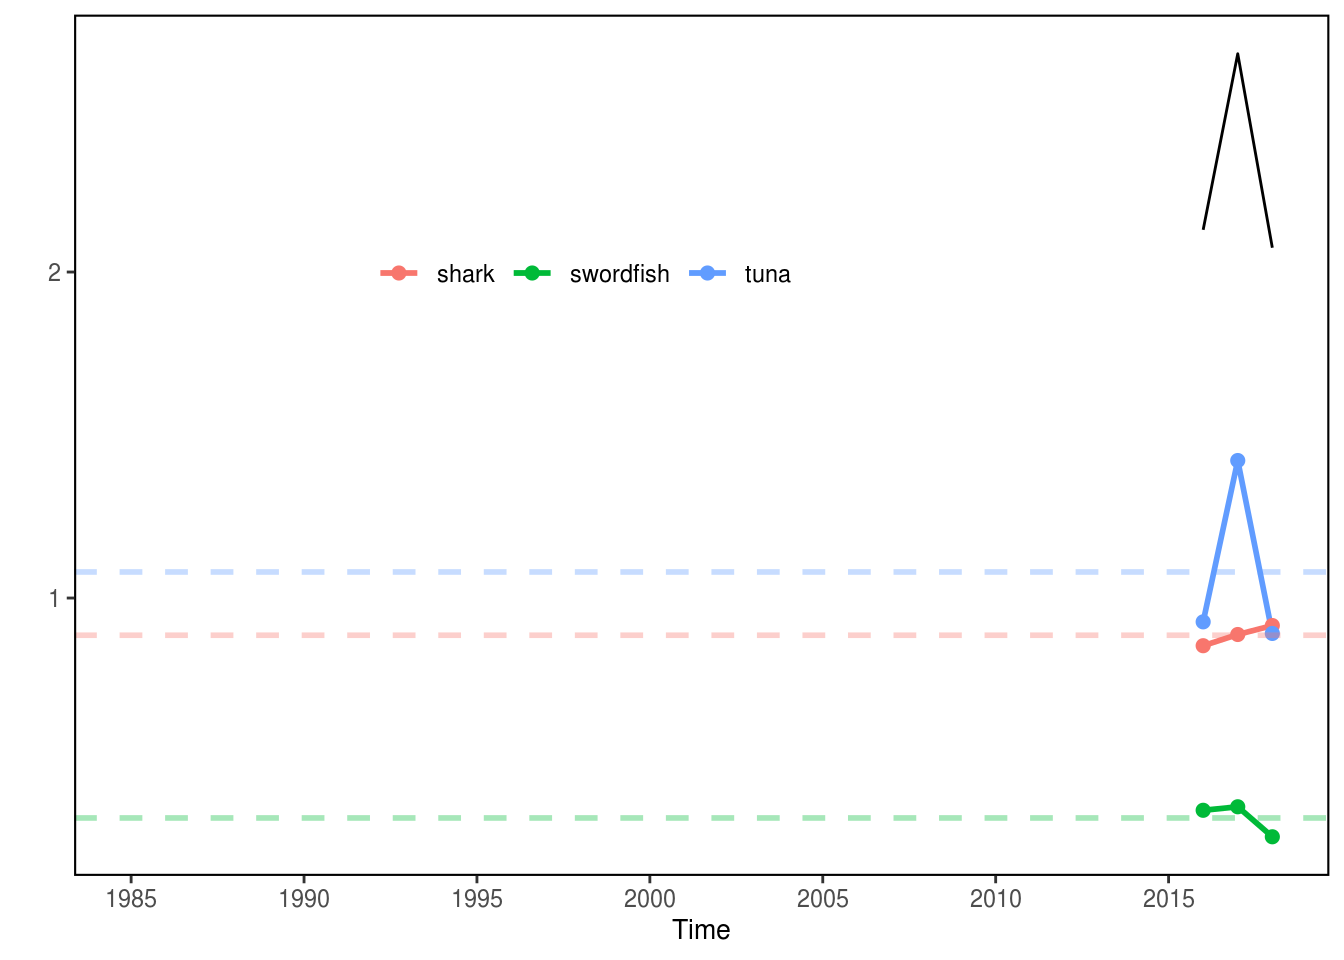
\includegraphics{/home/travis/build/NOAA-EDAB/tech-doc/images/unnamed-chunk-18-1.pdf}
\caption{\label{fig:unnamed-chunk-18}Highly migratory species landings from 2016-2018 grouped by sharks, tunas and swordfish.}
\end{figure}

\hypertarget{ichthyoplankton-diversity}{%
\chapter{Ichthyoplankton Diversity}\label{ichthyoplankton-diversity}}

\textbf{Description}: NOAA NEFSC Oceans and Climate branch public ichthyoplankton dataset

\textbf{Found in}: State of the Ecosystem - Gulf of Maine \& Georges Bank (2018, 2019), State of the Ecosystem - Mid-Atlantic (2018, 2019)

\textbf{Indicator category}: Database pull with analysis

\textbf{Contributor(s)}: Harvey J. Walsh

\textbf{Data steward}: Harvey Walsh, \href{mailto:harvey.walsh@noaa.gov}{\nolinkurl{harvey.walsh@noaa.gov}}

\textbf{Point of contact}: Harvey Walsh, \href{mailto:harvey.walsh@noaa.gov}{\nolinkurl{harvey.walsh@noaa.gov}}

\textbf{Public availability statement}: Source data are available to the public \href{ftp://ftp.nefsc.noaa.gov/pub/hydro/zooplankton_data/}{here}. Derived data for this indicator are available \href{https://comet.nefsc.noaa.gov/erddap/tabledap/ichthyo_div_soe_v1.html}{here}.

\hypertarget{methods-20}{%
\section{Methods}\label{methods-20}}

Data from the NOAA Northeast Fisheries Science Center (NEFSC) Oceans and Climate branch (OCB) public dataset were used to examine changes in diversity of abundance among 45 ichthyoplankton taxa. The 45 taxa were established (Walsh et al. \protect\hyperlink{ref-RN126}{2015}), and include the most abundant taxa from the 1970s to present that represent consistency in the identification of larvae.

\hypertarget{data-sources-20}{%
\subsection{Data sources}\label{data-sources-20}}

Multi-species plankton surveys cover the entire Northeast US shelf from Cape Hatteras, North Carolina, to Cape Sable, Nova Scotia, four to six times per year. A random-stratified design based on the NEFSC bottom trawl survey design (Azarovitz \protect\hyperlink{ref-Azarovitz1981}{1981}) is used to collect samples from 47 strata. The number of strata is lower than the trawl survey as many of the narrow inshore and shelf-break strata are combined in the EcoMon design.
The area encompassed by each stratum determined the number of samples in each stratum. Samples were collected both day and night using a 61 cm bongo net. Net tow speed was 1.5 knots and maximum sample depth was 200 m. Double oblique tows were a minimum of 5 mintues in duration, and fished from the surface to within 5 m of the seabed or to a maximum depth of 200 m. The volume filtered of all collections was measured with mechanical flowmeters mounted across the mouth of each net.

Processing of most samples was conducted at the Morski Instytut Rybacki (MIR) in Szczecin, Poland; the remaining samples were processed at the NEFSC or the Atlantic Reference Center, St Andrews, Canada. Larvae were identified to the lowest possible taxa and enumerated for each sample. Taxon abundance for each station was standardized to number under 10 m\textsuperscript{-2} sea surface.

\hypertarget{data-extraction-17}{%
\subsection{Data extraction}\label{data-extraction-17}}

Data retrieved from NOAA NEFSC Oceans and Climate branch \href{ftp://ftp.nefsc.noaa.gov/pub/hydro/zooplankton_data/}{public dataset}
(Filename: ``EcoMon\_Plankton\_Data\_v3\_0.xlsx'', File Date: 10/20/2016).

\hypertarget{data-analysis-19}{%
\subsection{Data analysis}\label{data-analysis-19}}

All detailed data processing steps are not currently included in this document, but general steps are outlined. Data were grouped into seasons: spring = February, March, April and fall = September, October, November. Stratified weighted mean abundance was calculated for each taxon for each year and season across all plankton strata (n = 47) for 17 years (1999 to 2015). Shannon Diversity Index and count of positive taxon was calculated for each season and year.

MATLAB code used to calculate diversity indices can be found using this \href{https://github.com/NOAA-EDAB/tech-doc/tree/master/R/stored_scripts/ich_div_analysis}{link}.

\hypertarget{data-processing-14}{%
\subsection{Data processing}\label{data-processing-14}}

Ichthyoplankton diversity data sets were formatted for inclusion in the \texttt{ecodata} R package using the R code found \href{https://github.com/NOAA-EDAB/ecodata/blob/master/data-raw/get_ichthyoplankton.R}{here}.

\hypertarget{plotting-13}{%
\subsection{Plotting}\label{plotting-13}}

Code used to plot ichthyoplankton diversity can be found \href{https://github.com/NOAA-EDAB/tech-doc/tree/master/R/stored_scripts/ich_div_plotting.R}{here}.

\hypertarget{inshoresurvdat}{%
\chapter{Inshore bottom trawl surveys}\label{inshoresurvdat}}

\textbf{Description}: Inshore surveys include the Northeast Area Monitoring and Assessment Program (NEAMAP) survey, Massachusetts Division of Marine Fisheries Bottom Trawl Survey, and Maine/New Hampshire Inshore Trawl Survey.

\textbf{Indicator category}: Database pull with analysis

\textbf{Found in}: State of the Ecosystem - Mid-Atlantic (2019,2020), State of the Ecosystem - New England (2019, 2020)

\textbf{Contributor(s)}: James Gartland, Matt Camisa, Rebecca Peters, Sean Lucey

\textbf{Data steward}: Kimberly Bastille, \href{mailto:kimberly.bastille@noaa.gov}{\nolinkurl{kimberly.bastille@noaa.gov}}

\textbf{Points of contact}: James Gartland (NEAMAP), \href{mailto:jgartlan@vims.edu}{\nolinkurl{jgartlan@vims.edu}}; Rebecca Peters (ME/NH survey), \href{mailto:rebecca.j.peters@maine.gov}{\nolinkurl{rebecca.j.peters@maine.gov}}; Sean Lucey (MA Inshore Survey), \href{mailto:sean.lucey@noaa.gov}{\nolinkurl{sean.lucey@noaa.gov}}

\textbf{Public availability statement}: Data are available upon request.

\hypertarget{methods-21}{%
\section{Methods}\label{methods-21}}

\hypertarget{data-sources-21}{%
\subsection{Data Sources}\label{data-sources-21}}

All inshore bottom trawl survey data sets were derived from raw survey data. NEAMAP source data are available for download \href{https://www.vims.edu/research/departments/fisheries/programs/multispecies_fisheries_research/abundance_indices/index.php}{here}. More detailed information describing NEAMAP survey methods is available on the \href{http://neamap.net}{NEAMAP website}. ME/NH inshore survey data are available upon request (see Points of Contact). Technical documentation for ME/NH survey methods and survey updates are made available through the \href{https://www.maine.gov/dmr/science-research/projects/trawlsurvey/index.html}{Maine Department of Marine Resources}. Data from the MA Inshore Bottom Trawl Survey are stored on local servers at the Northeast Fisheries Science Center (Woods Hole, MA), and are also available upon request. More information about the MA Inshore Bottom Trawl Survey is available \href{https://www.mass.gov/service-details/review-trawl-survey-updates}{here}.

\hypertarget{data-extraction-18}{%
\subsection{Data extraction}\label{data-extraction-18}}

Source data from the Massachusetts DMF Bottom Trawl Survey were extracted using this \href{https://github.com/slucey/RSurvey/blob/master/Mass_survey.R}{R script}.

\hypertarget{data-processing-15}{%
\subsection{Data Processing}\label{data-processing-15}}

The following R code was used to process inshore bottom trawl data into the \texttt{ecodata} R package.

\textbf{New England}

\url{https://github.com/NOAA-EDAB/ecodata/blob/master/data-raw/get_inshore_survdat.R}

\textbf{Massachusetts}

\url{https://github.com/NOAA-EDAB/ecodata/blob/master/data-raw/get_mass_inshore_survey.R}

\textbf{Mid-Atlantic (NEAMAP)}

\url{https://github.com/NOAA-EDAB/ecodata/blob/master/data-raw/get_mab_inshore_survey.R}

\hypertarget{data-analysis-20}{%
\subsection{Data Analysis}\label{data-analysis-20}}

Biomass indices were provided as stratified mean biomass (kg tow\textsuperscript{-1}) for all inshore surveys. Time series of stratified mean biomass were calculated for ME/NH and NEAMAP surveys through the following procedure:

\begin{enumerate}
\def\labelenumi{\arabic{enumi}.}
\tightlist
\item
  All species catch weights were summed for each tow and for each feeding guild category.
\item
  The average weight per tow, associated variances and standard deviation for each survey, region, stratum, and feeding guild was calculated.
\item
  Stratified mean biomass was then calculated as the sum of the weighted averages of the strata, where the weight of a given stratum was the proportion of the survey area accounted for by that stratum.
\end{enumerate}

Stratified mean biomass was also calculated for the MA Inshore Bottom Trawl Survey. These calculations followed those used to find stratified mean biomass by feeding guild in the NEFSC Bottom Trawl Survey and are described in greater detail \protect\hyperlink{survdat}{here}. The R code used to derive the stratified mean biomass indices for MA Inshore time series is provided below.

R code used for analysis can be found \href{https://github.com/NOAA-EDAB/tech-doc/blob/master/R/stored_scripts/inshore_survey_analysis.R}{here}.

\hypertarget{plotting-14}{%
\subsection{Plotting}\label{plotting-14}}

\hypertarget{neamap}{%
\subsubsection{\texorpdfstring{\href{https://github.com/NOAA-EDAB/ecodata/blob/master/chunk-scripts/macrofauna.Rmd-agg-bio.R}{NEAMAP}}{NEAMAP}}\label{neamap}}

\begin{figure}
\centering
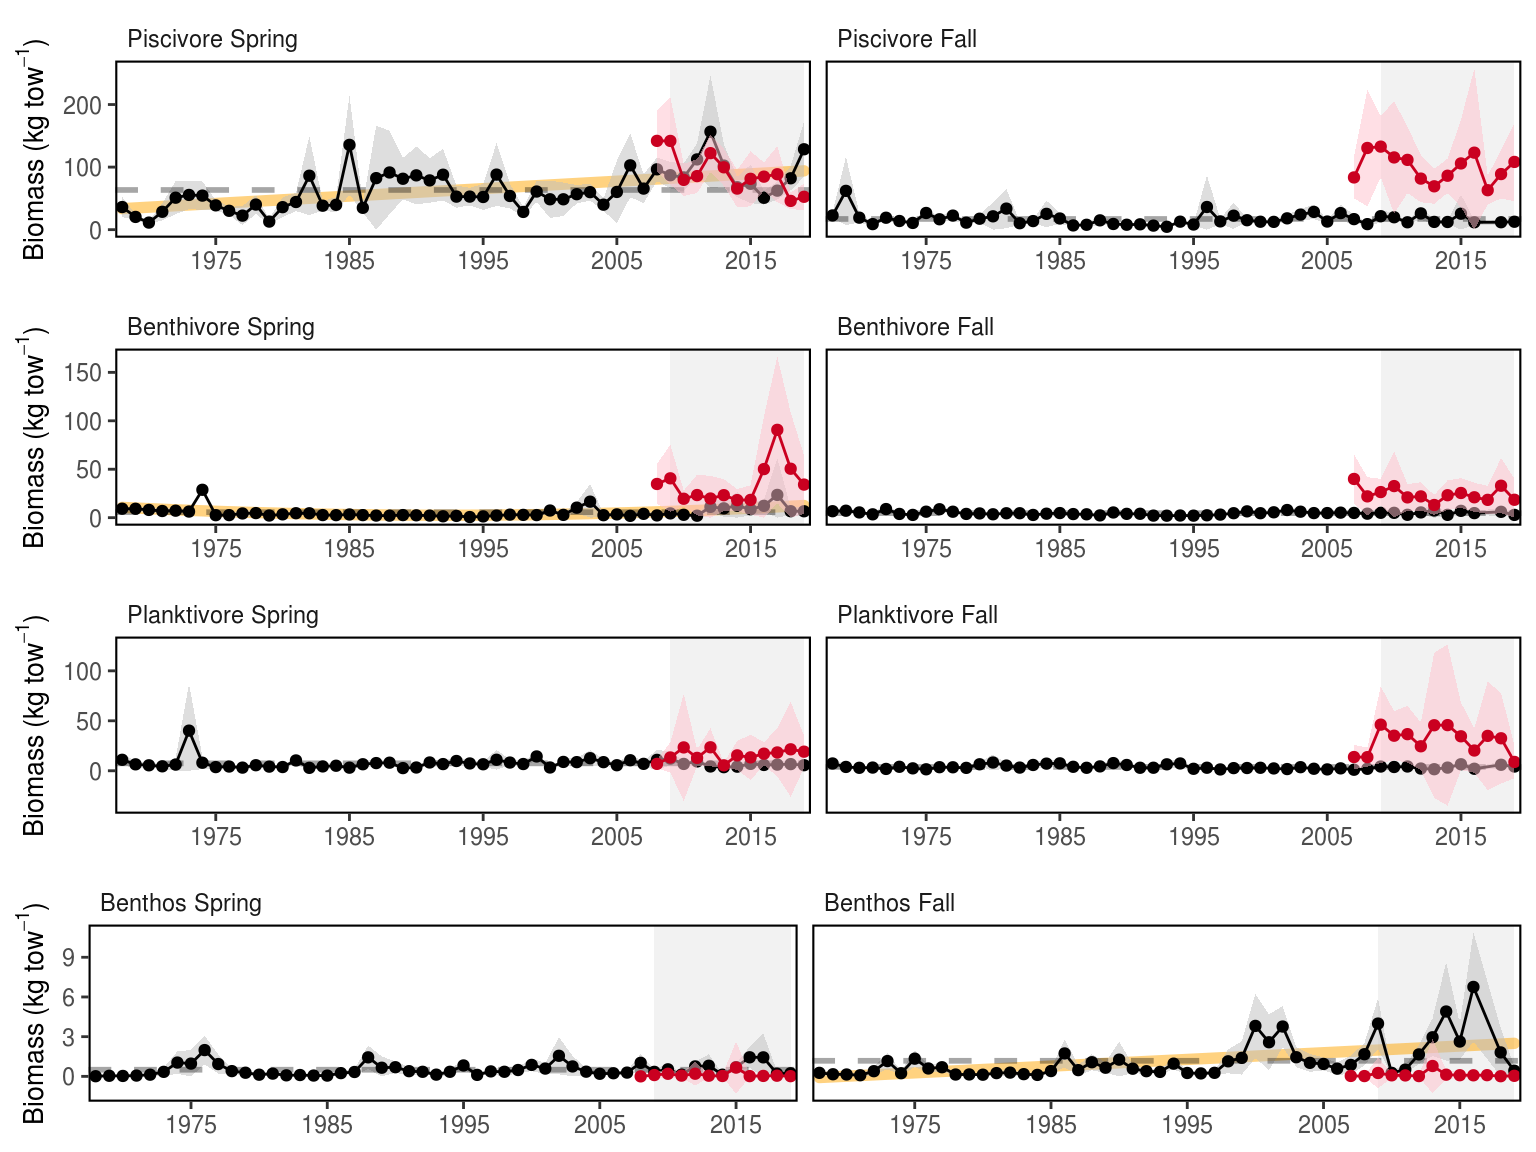
\includegraphics{/home/travis/build/NOAA-EDAB/tech-doc/images/unnamed-chunk-19-1.pdf}
\caption{\label{fig:unnamed-chunk-19}Spring (left) and fall (right) surveyed biomass in the Mid-Atlantic Bight. Data from the NEFSC Bottom Trawl Survey are shown in black, with NEAMAP shown in red.}
\end{figure}

\hypertarget{massechusetts}{%
\subsubsection{\texorpdfstring{\href{https://github.com/NOAA-EDAB/ecodata/blob/master/chunk-scripts/macrofauna.Rmd-MA-inshore.R}{Massechusetts}}{Massechusetts}}\label{massechusetts}}

\begin{figure}
\centering
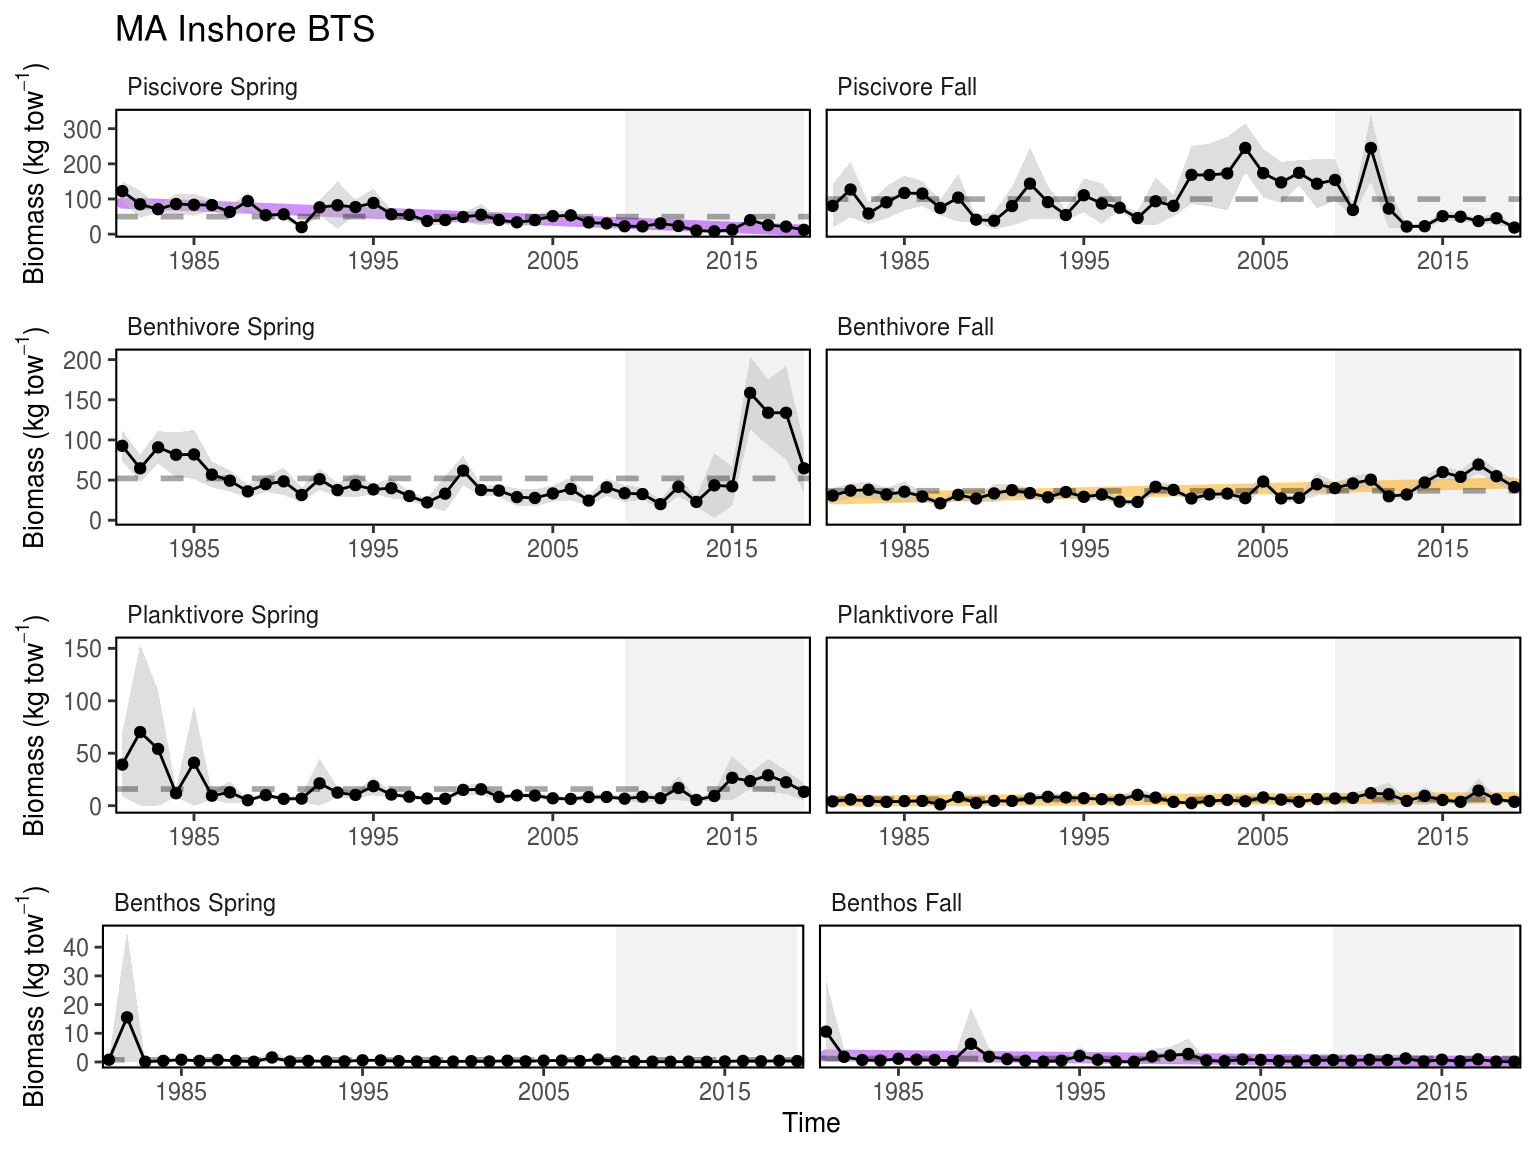
\includegraphics{/home/travis/build/NOAA-EDAB/tech-doc/images/unnamed-chunk-20-1.pdf}
\caption{\label{fig:unnamed-chunk-20}Spring (left) and fall (right) surveyed biomass from the MA state inshore bottom trawl survey.}
\end{figure}

\hypertarget{maine-new-hampshire}{%
\subsubsection{\texorpdfstring{\href{https://github.com/NOAA-EDAB/ecodata/blob/master/chunk-scripts/macrofauna.Rmd-menh-survey.R}{Maine-New Hampshire}}{Maine-New Hampshire}}\label{maine-new-hampshire}}

\begin{figure}
\centering
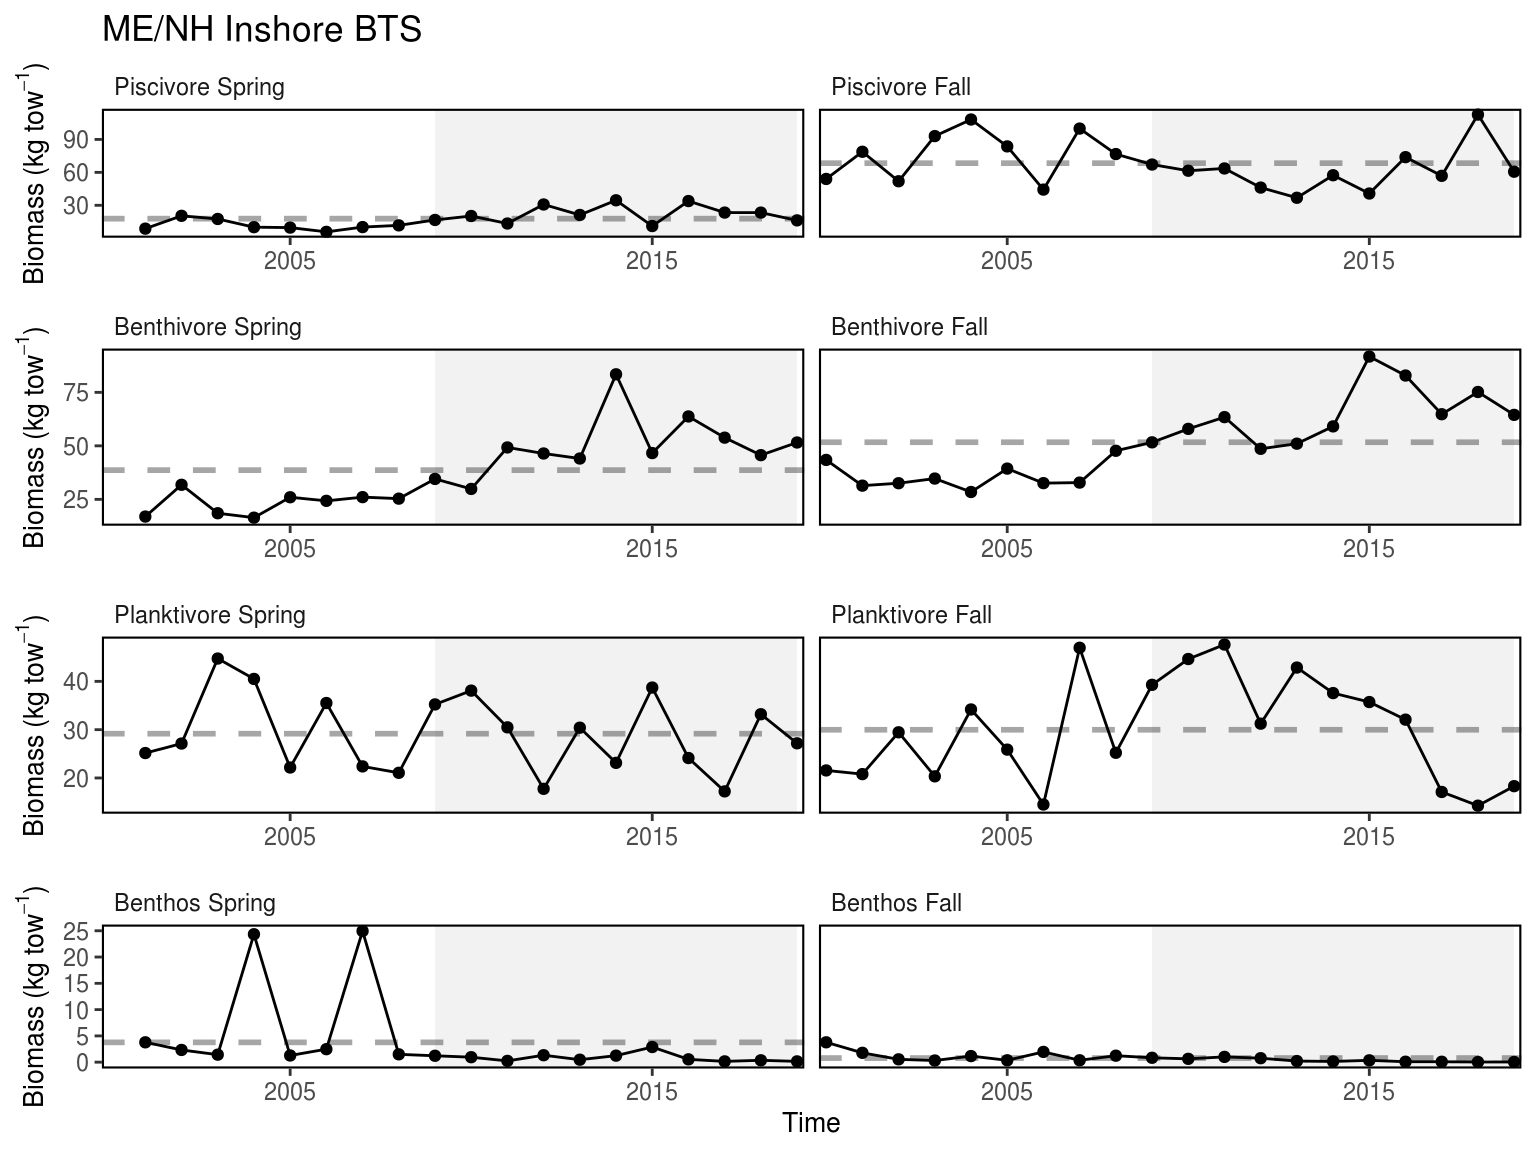
\includegraphics{/home/travis/build/NOAA-EDAB/tech-doc/images/unnamed-chunk-21-1.pdf}
\caption{\label{fig:unnamed-chunk-21}Spring (left) and fall(right) surveyed biomass from the ME/NH state inshore bottom trawl survey.}
\end{figure}

\hypertarget{long-term-sea-surface-temperature}{%
\chapter{Long-term Sea Surface Temperature}\label{long-term-sea-surface-temperature}}

\textbf{Description}: Long-term sea-surface temperatures

\textbf{Found in}: State of the Ecosystem - Gulf of Maine \& Georges Bank (2017, 2018, 2019, 2020), State of the Ecosystem - Mid-Atlantic (2017, 2018, 2019, 2020)

\textbf{Indicator category}: Database pull

\textbf{Contributor(s)}: Kevin Friedland

\textbf{Data steward}: Kevin Friedland, \href{mailto:kevin.friedland@noaa.gov}{\nolinkurl{kevin.friedland@noaa.gov}}

\textbf{Point of contact}: Kevin Friedland, \href{mailto:kevin.friedland@noaa.gov}{\nolinkurl{kevin.friedland@noaa.gov}}

\textbf{Public availability statement}: Source data are available \href{https://www.esrl.noaa.gov/psd/data/gridded/data.noaa.ersst.v5.html}{here}.

\hypertarget{methods-22}{%
\section{Methods}\label{methods-22}}

Data for long-term sea-surface temperatures were derived from the Noational Oceanographic and Atmospheric Administration (NOAA) extended reconstructed sea surface temperature data set (ERSST V5). The ERSST V5 dataset is parsed into 2° x 2° gridded bins between 1854-present with monthly temporal resolution. Data were interpolated in regions with limited spatial coverage, and heavily damped during the period between 1854-1880 when collection was inconsistent (Huang, Thorne, et al. \protect\hyperlink{ref-Huang2017}{2017}\protect\hyperlink{ref-Huang2017}{a}, \protect\hyperlink{ref-huang2017extended}{2017}\protect\hyperlink{ref-huang2017extended}{b}). For this analysis, 19 bins were selected that encompassed the Northeast US Continental Shelf region (see Friedland and Hare \protect\hyperlink{ref-Friedland2007}{2007}).

\hypertarget{data-sources-22}{%
\subsection{Data sources}\label{data-sources-22}}

This indicator is derived from the \href{https://www.esrl.noaa.gov/psd/data/gridded/data.noaa.ersst.v5.html}{NOAA ERSST V5 dataset} (Huang, Thorne, et al. \protect\hyperlink{ref-Huang2017}{2017}\protect\hyperlink{ref-Huang2017}{a}).

\hypertarget{data-extraction-19}{%
\subsection{Data extraction}\label{data-extraction-19}}

\begin{table}

\caption{\label{tab:coordinates}Coordinates used in NOAA ERSST V5 data extraction.}
\centering
\begin{tabular}[t]{rr}
\toprule
Longitude & Latitude\\
\midrule
-74 & 40\\
-74 & 38\\
-72 & 40\\
-70 & 44\\
-70 & 42\\
\addlinespace
-70 & 40\\
-68 & 44\\
-68 & 42\\
\bottomrule
\end{tabular}
\end{table}

R code used in extracting time series of long-term SST data can be found \href{https://github.com/NOAA-EDAB/tech-doc/tree/master/R/stored_scripts/long-term-sst-extraction.R}{here}.

\hypertarget{data-processing-16}{%
\subsection{Data Processing}\label{data-processing-16}}

Data were formatted for inclusion in the \texttt{ecodata} R package with the R code found \href{https://github.com/NOAA-EDAB/ecodata/blob/master/data-raw/get_long_term_sst.R}{here}.

\hypertarget{plotting-15}{%
\subsection{Plotting}\label{plotting-15}}

The plot below was built using the code found
\href{https://github.com/NOAA-EDAB/ecodata/blob/master/chunk-scripts/LTL.Rmd-long-term-sst.R}{here}.

\begin{figure}

{\centering 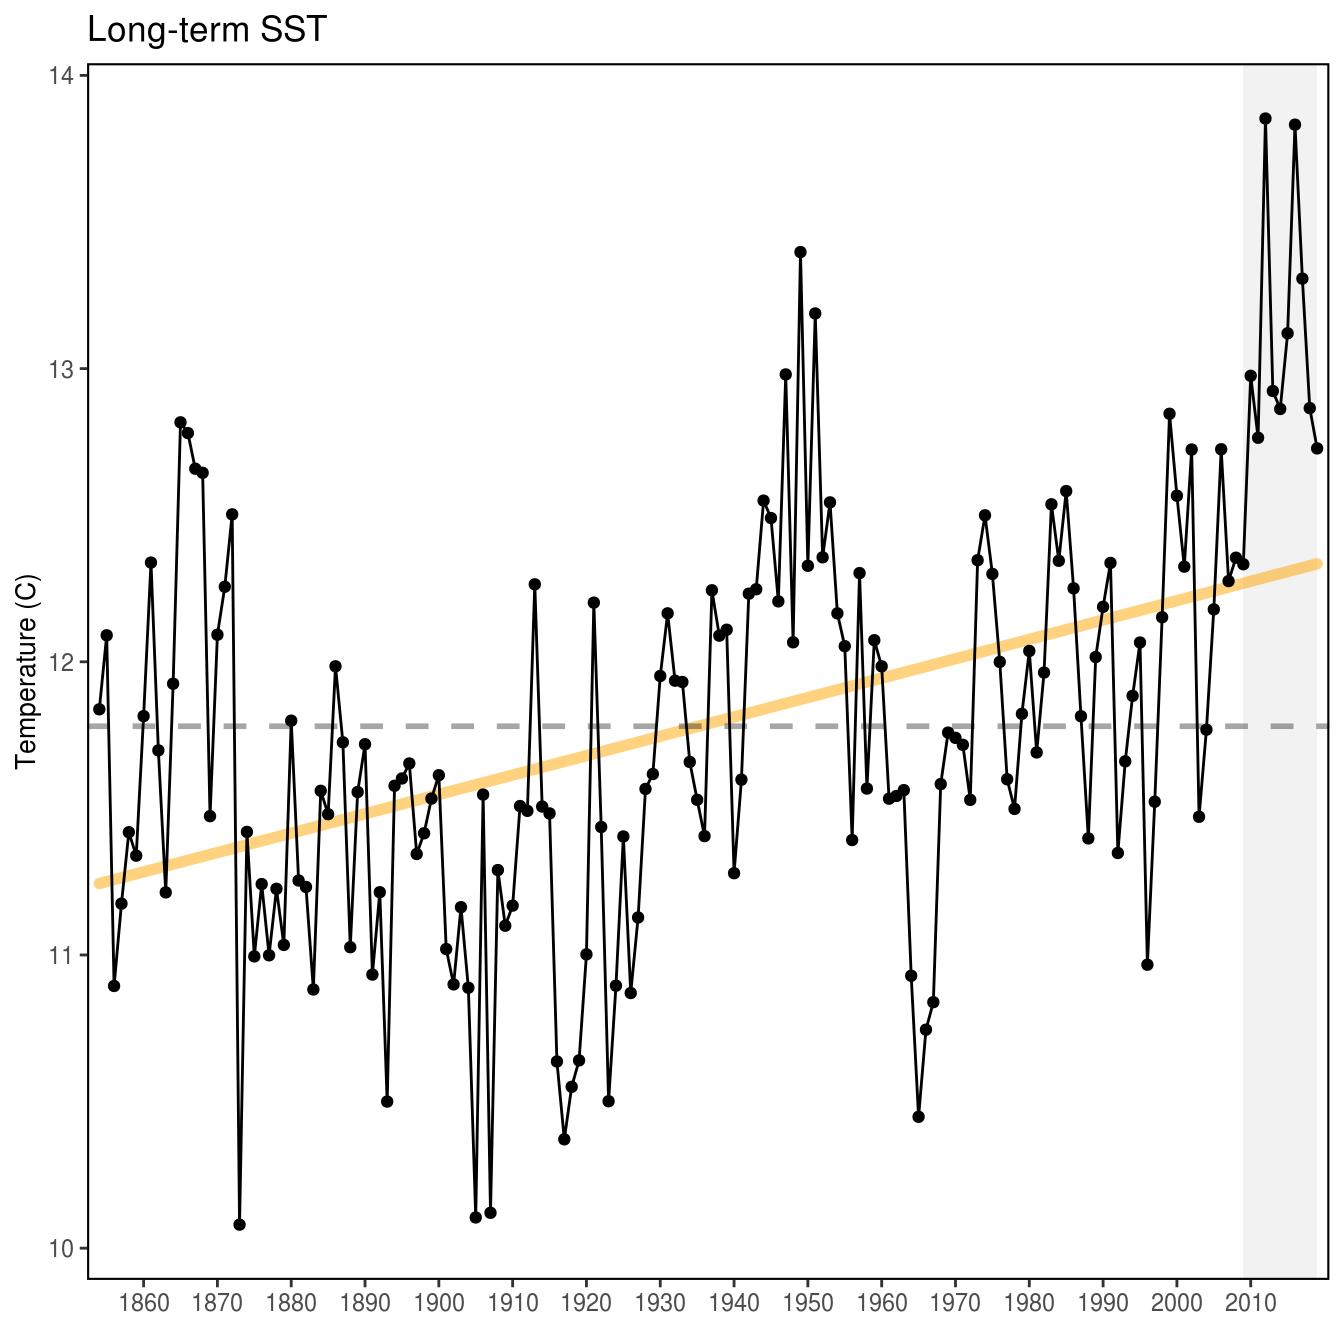
\includegraphics{/home/travis/build/NOAA-EDAB/tech-doc/images/unnamed-chunk-22-1} 

}

\caption{Long-term sea surface temperatures on the Northeast Continental Shelf.}\label{fig:unnamed-chunk-22}
\end{figure}

\hypertarget{mid-atlantic-harmful-algal-bloom-indicator}{%
\chapter{Mid-Atlantic Harmful Algal Bloom Indicator}\label{mid-atlantic-harmful-algal-bloom-indicator}}

\textbf{Description}: An aggregation of reported algal bloom data in Chesapeake Bay between 2007-2017.

\textbf{Found in}: State of the Ecosystem - Mid-Atlantic (2018)

\textbf{Indicator category}: Database pull

\textbf{Contributor(s)}: Sean Hardison, Virginia Department of Health

\textbf{Data steward}: Kimberly Bastille, \href{mailto:kimberly.bastille@noaa.gov}{\nolinkurl{kimberly.bastille@noaa.gov}}

\textbf{Point of contact}: Kimberly Bastille, \href{mailto:kimberly.bastille@noaa.gov}{\nolinkurl{kimberly.bastille@noaa.gov}}

\textbf{Public availability statement}: Source data for this indicator are available \href{https://github.com/NOAA-EDAB/tech-doc/tree/master/data/CB_HAB}{here}. Processed time series can be found \href{http://comet.nefsc.noaa.gov/erddap/tabledap/CBhabs_ann_soe_v2.html}{here}.

\hypertarget{methods-23}{%
\section{Methods}\label{methods-23}}

We presented two indicator time series for reports of algal blooms in the southern portion of Chesapeake Bay between 2007-2017. The first indicator was observations of algal blooms above 5000 cell ml\textsuperscript{-1}. This threshold was developed by the Virginia Department of Health (VDH) for \emph{Microcystis} spp. algal blooms based on World Health Organization guidelines (Organization \protect\hyperlink{ref-WHO2003}{2003}; Health \protect\hyperlink{ref-VDH2011}{2011}). VDH also uses this same threshold for other algal species blooms in Virginia waters. When cell concentrations are above 5000 cell ml\textsuperscript{-1}, VDH recommends initiation of biweekly water sampling and that relevant local agencies be notified of the elevated cell concentrations.

The second indicator we reported, blooms of \emph{Cochlodinium polykrikoides} at cell concentrations \textgreater300 cell ml\textsuperscript{-1}, was chosen due to reports of high ichthyotoxicity seen at these levels. Tang and Gobler (\protect\hyperlink{ref-Tang2009}{2009}) showed that fish exposed to cultured \emph{C. polykrikoides} at densities as low 330 cells ml\textsuperscript{-1} saw 100\% mortality within 1 hour, which if often far less than \emph{C. polykrikoides} cell concentrations seen in the field. Algal bloom data were not available for 2015 nor 2010. The algal bloom information presented here are a synthesis of reported events, and has been updated to include data not presented in the 2018 State of the Ecosystem Report.

\hypertarget{data-sources-23}{%
\subsection{Data sources}\label{data-sources-23}}

Source data were obtained from VDH. Sampling, identification, and bloom characterization was completed by the VDH, Phytoplankton Analysis Laboratory at Old Dominion University (ODU), Reece Lab at the Virginia Institute of Marine Science (VIMS), and Virginia Department of Environmental Quality. Problem algal species were targeted for identification via light microscopy followed by standard or quantitative PCR assays and/or enzyme-linked immunosorbent assay (ELISA). Reports specifying full methodologies from ODU, VIMS, and VDH source data are available upon request.

\hypertarget{data-extraction-20}{%
\subsection{Data extraction}\label{data-extraction-20}}

Data were extracted from a series of spreadsheets provided by the VDH. We quantified the number of algal blooms in each year reaching target cell density thresholds in the southern Chesapeake Bay.



R code used in extracting harmful algal bloom data can be found \href{https://github.com/NOAA-EDAB/tech-doc/tree/master/R/stored_scripts/mab_hab_extraction.R}{here}.

\hypertarget{data-analysis-21}{%
\subsection{Data analysis}\label{data-analysis-21}}

No data analysis steps took place for this indicator.

\hypertarget{new-england-harmful-algal-bloom-indicator}{%
\chapter{New England Harmful Algal Bloom Indicator}\label{new-england-harmful-algal-bloom-indicator}}

\textbf{Description}: Regional incidence of shellfish bed closures due to presence of toxins associated with harmful algae.

\textbf{Found in}: State of the Ecosystem - Gulf of Maine \& Georges Bank (2018)

\textbf{Indicator Category}: Synthesis of published information

\textbf{Contributor(s)}: Dave Kulis, Donald M Anderson, Sean Hardison

\textbf{Data steward}: Kimberly Bastille, \href{mailto:kimberly.bastille@noaa.gov}{\nolinkurl{kimberly.bastille@noaa.gov}}

\textbf{Point of contact}: Kimberly Bastille, \href{mailto:kimberly.bastille@noaa.gov}{\nolinkurl{kimberly.bastille@noaa.gov}}

\textbf{Public availability statement}: Data are publicly available (see Data Sources below).

\hypertarget{methods-24}{%
\section{Methods}\label{methods-24}}

The New England Harmful Algal Bloom (HAB) indicator is a synthesis of shellfish bed closures related to the presence of HAB-associated toxins above threshold levels from 2007-2016 (Figure \ref{fig:NE-HAB}). Standard detection methods were used to identify the presence of toxins associated with Amnesic Shellfish Poisoning (ASP), Paralytic Shellfish Poisoning (PSP), and Diarrhetic Shellfish Poisoning (DSP) by state and federal laboratories.

\hypertarget{paralytic-shellfish-poisoning}{%
\subsubsection{Paralytic Shellfish Poisoning}\label{paralytic-shellfish-poisoning}}

The most common cause of shellfish bed closures in New England is the presence of paralytic shellfish toxins (PSTs) produced by the dinoflagellate \emph{Alexandrium catenella}. All New England states except Maine relied on the Association of Official Analytical Chemists (AOAC) approved mouse bioassay method to detect PSTs in shellfish during the 2007-2016 period reported here (International \protect\hyperlink{ref-Anonymous2005}{2005}).

In Maine, PST detection methods were updated in May 2014 when the state adopted the hydrophilic interaction liquid chromatography (HILIC) UPLC-MS/MS protocol (Boundy et al. \protect\hyperlink{ref-Boundy2015}{2015}) in concordance with National Shellfish Sanitation Program (NSSP) requirements. Prior to this, the primary method used to detect PST in Maine was with the mouse bioassay.

\hypertarget{amnesic-shellfish-poisoning}{%
\subsubsection{Amnesic Shellfish Poisoning}\label{amnesic-shellfish-poisoning}}

Amnesic shellfish poisoning (ASP) is caused by the toxin domoic acid (DA), which is produced by several phytoplankton species belonging to the genus \emph{Pseudo-nitzchia}. In New England, a UV-HPLC method (Quilliam, Xie, and Hardstaff \protect\hyperlink{ref-Quilliam1995}{1995}), which specifies a HPLC-UV protocol, is used for ASP detection.

\hypertarget{diarrhetic-shellfish-poisoning}{%
\subsubsection{Diarrhetic Shellfish Poisoning}\label{diarrhetic-shellfish-poisoning}}

Diarrhetic Shellfish Poisoning (DSP) is rare in New England waters, but the presence of the DSP-associated okadaic acid (OA) in mussels was confirmed in Massachusetts in 2015 (J. Deeds, personal communication, July 7, 2018). Preliminary testing for OA in Massachusetts utilized the commercially available Protein Phosphatase Inhibition Assay (PPIA) and these results are confirmed through LC-MS/MS when necessary (Smienk et al. \protect\hyperlink{ref-Smienk2012}{2012}; Stutts and Deeds \protect\hyperlink{ref-Stutts2017}{2017}).

\hypertarget{data-sources-24}{%
\subsection{Data sources}\label{data-sources-24}}

Data used in this indicator were drawn from the 2017 Report on the ICES-IOC Working Group on Harmful Algal Bloom Dynamics (WGHABD). The report and data are available \href{http://www.ices.dk/sites/pub/Publication\%20Reports/Expert\%20Group\%20Report/SSGEPD/2017/01\%20WGHABD\%20-\%20Report\%20of\%20the\%20ICES\%20-\%20IOC\%20Working\%20Group\%20on\%20Harmful\%20Algal\%20Bloom\%20Dynamics.pdf}{here}.

Closure information was collated from information provided by the following organizations:

\begin{table}

\caption{\label{tab:closuresrc}Shellfish closure information providers.}
\centering
\begin{tabular}[t]{ll}
\toprule
State & Source Organization\\
\midrule
Maine & Maine Department of Marine Resources\\
New Hampshire & New Hampshire Department of Environmental Services\\
Massachusetts & Massachusetts Division of Marine Fisheries\\
Rhode Island & Rhode Island Department of Environmental Management\\
Connecticut & Connecticut Department of Agriculture\\
\bottomrule
\end{tabular}
\end{table}

\hypertarget{data-extraction-21}{%
\subsection{Data extraction}\label{data-extraction-21}}

Data were extracted from the original report visually and accuracy confirmed with report authors.

\hypertarget{data-analysis-22}{%
\subsection{Data analysis}\label{data-analysis-22}}

No data analysis steps took place for this indicator.

\hypertarget{plotting-16}{%
\subsection{Plotting}\label{plotting-16}}

The script used to develop the figure in the SOE report can be found \href{https://github.com/NOAA-EDAB/tech-doc/tree/master/R/stored_scripts/ne_hab_plotting.R}{here}.

\hypertarget{marine-heatwave}{%
\chapter{Marine Heatwave}\label{marine-heatwave}}

\textbf{Description}: Marine Heatwave

\textbf{Found in}: State of the Ecosystem - Gulf of Maine \& Georges Bank (2020), Mid-Atlantic (2020)

\textbf{Indicator category}: Published methods, Database pull with analysis

\textbf{Contributor(s)}: Vincent Saba

\textbf{Data steward}: Kimberly Bastille \href{mailto:kimberly.bastille@noaa.gov}{\nolinkurl{kimberly.bastille@noaa.gov}}

\textbf{Point of contact}: Vincent Saba \href{mailto:vincent.saba@noaa.gov}{\nolinkurl{vincent.saba@noaa.gov}}

\textbf{Public availability statement}:

\hypertarget{methods-25}{%
\section{Methods}\label{methods-25}}

Marine heatwave analysis for Georges Bank, Gulf of Maine, and the Middle Atlantic Bight according to the definition in Hobday et al. (\protect\hyperlink{ref-hobday2016}{2016}).

\hypertarget{data-sources-25}{%
\subsection{Data sources}\label{data-sources-25}}

NOAA high-res OISST (daily, 25-km, 1982-2019) \url{https://www.esrl.noaa.gov/psd/cgi-bin/db_search/DBListFiles.pl?did=132\&tid=79458\&vid=2423}

\hypertarget{data-extraction-22}{%
\subsection{Data extraction}\label{data-extraction-22}}

Each yearly file (global) was downloaded, concatenated into a single netcdf file using nco (Unix), and then cropped to the USNES region using Ferret. Each EPU's time-series of SST was averaged using .shp file boundaries for the MAB, GB, and GOM (also done in Ferret) and saved to the three .csv files.

\hypertarget{data-analysis-23}{%
\subsection{Data analysis}\label{data-analysis-23}}

The marine heatwave metrics Maximum Intensity {[}deg. C{]} and Cumulative Intensity {[}deg. C x days{]} are calculated using NOAA OISST daily sea surface temperature data (25-km resolution) from January 1982 to December 2019. The heatwaves are calculated based on the algorithms in Hobday et al.~2016 and by using a climatology of 1982-2010. These metrics were run R using \url{https://robwschlegel.github.io/heatwaveR/}

\hypertarget{data-processing-17}{%
\subsection{Data processing}\label{data-processing-17}}

Marine Heatwave data were formatted for inclusion in the \texttt{ecodata} R package using this \href{https://github.com/NOAA-EDAB/ecodata/blob/master/data-raw/get_heatwave.R}{R code}.

\hypertarget{plotting-17}{%
\subsection{Plotting}\label{plotting-17}}

Code used for the plots below can be found \href{https://github.com/NOAA-EDAB/ecodata/blob/master/chunk-scripts/LTL.Rmd-heatwave_mab.R}{here}.

\begin{figure}

{\centering 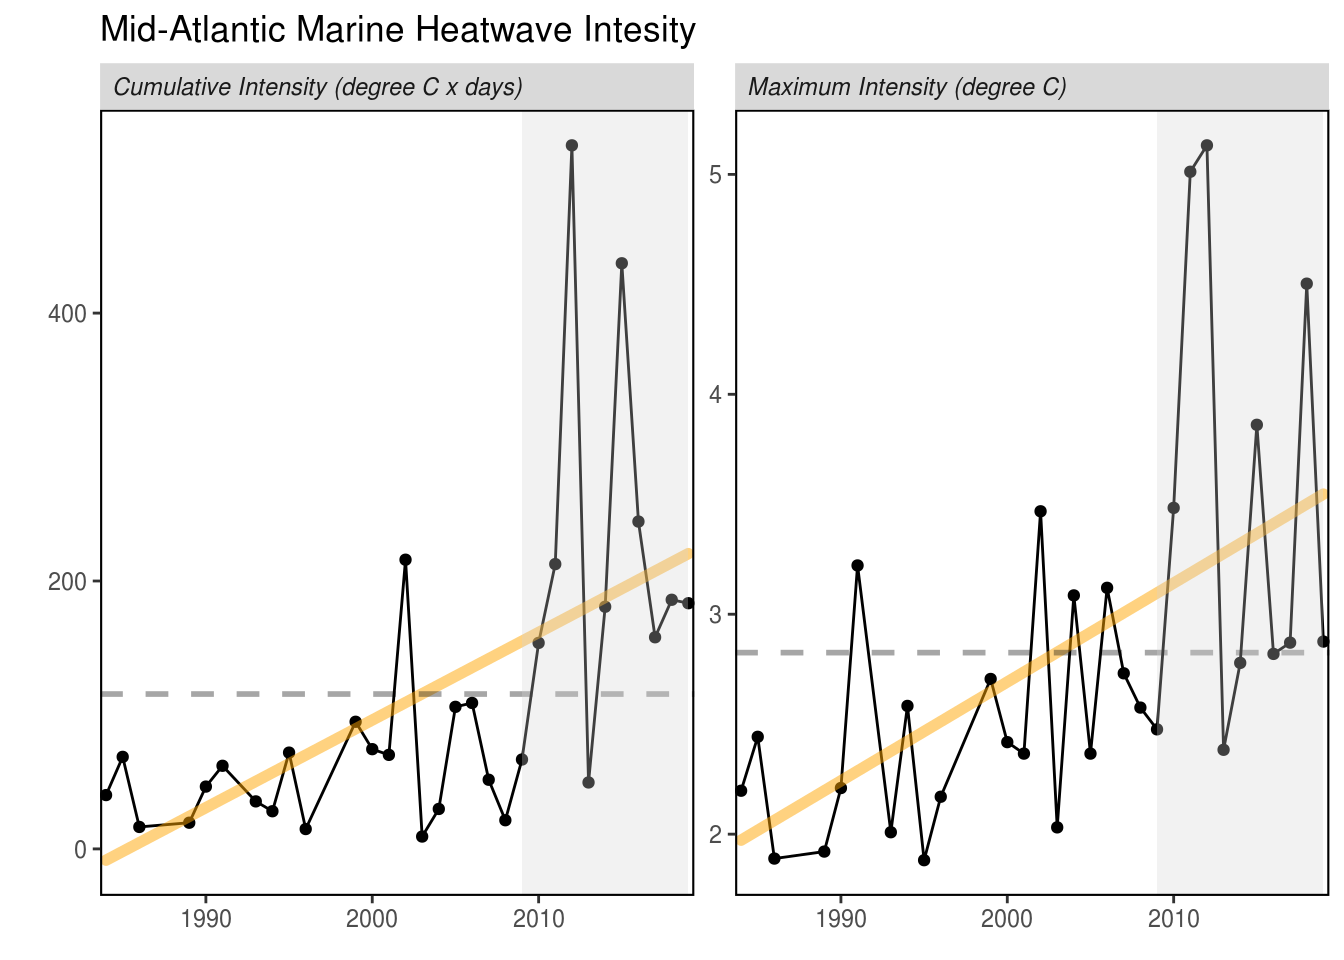
\includegraphics{/home/travis/build/NOAA-EDAB/tech-doc/images/unnamed-chunk-24-1} 

}

\caption{Cumulative and maximum marine heatwave in the Mid-Atlantic}\label{fig:unnamed-chunk-24}
\end{figure}

\begin{figure}
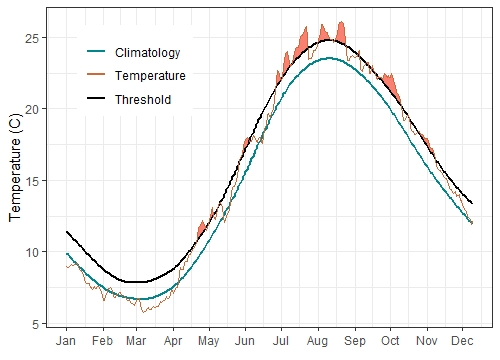
\includegraphics[width=1\linewidth]{/home/travis/build/NOAA-EDAB/tech-doc/images/mab_heatwave} \caption{Heatwave events in 2019.}\label{fig:unnamed-chunk-25}
\end{figure}

\begin{figure}

{\centering 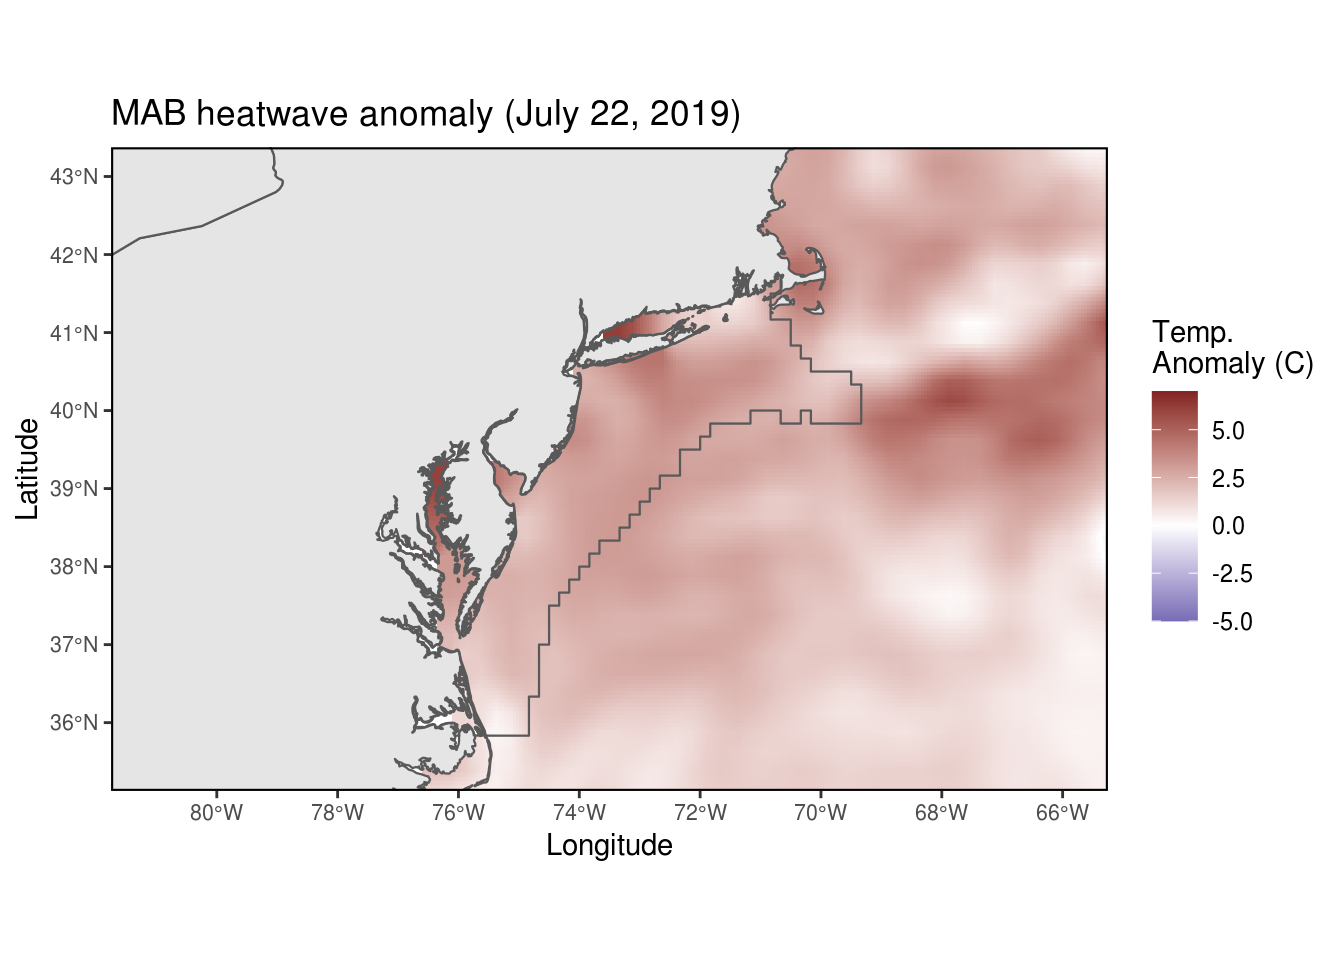
\includegraphics{/home/travis/build/NOAA-EDAB/tech-doc/images/unnamed-chunk-26-1} 

}

\caption{Map showing the maximum intensity heatwave in the Mid-Atlantic occuring on July 22, 2019}\label{fig:unnamed-chunk-26}
\end{figure}

\hypertarget{verified-records-of-southern-kingfish}{%
\chapter{Verified Records of Southern Kingfish}\label{verified-records-of-southern-kingfish}}

\textbf{Description}: Fisheries Observer Data -- Verified Records of Southern Kingfish

\textbf{Found in}: State of the Ecosystem - Mid-Atlantic (2018)

\textbf{Indicator category}: Database pull

\textbf{Contributor(s)}: Debra Duarte, Loren Kellogg

\textbf{Data steward}: Gina Shield, \href{mailto:gina.shield@noaa.gov}{\nolinkurl{gina.shield@noaa.gov}}

\textbf{Point of contact}: Gina Shield, \href{mailto:gina.shield@noaa.gov}{\nolinkurl{gina.shield@noaa.gov}}

\textbf{Public availability statement}: Due to PII concerns data for this indicator are not publicly available.

\hypertarget{methods-26}{%
\section{Methods}\label{methods-26}}

\hypertarget{data-sources-26}{%
\subsection{Data sources}\label{data-sources-26}}

The Fisheries Sampling Branch deploys observers on commercial fisheries trips from Maine to North Carolina. On observed tows, observers must fully document all kept and discarded species encountered. Observers must comply with a Species Verification Program (SVP), which requires photo or sample submissions of high priority species at least once per quarter. Photos and samples submitted for verification are identified independently by at least two reviewers.

The derived data presented in the Mid-Atlantic State of the Ecosystem report for southern kingfish include records verified by the SVP program only. The occurrence of southern kingfish in SVP records were chosen for inclusion in the report due to the recent increases of the species in SVP observer records since 2010. These data are not a complete list from the New England Fisheries Observer Program (NEFOP). Southern Kingfish are less common than Northern Kingfish in observer data and are possibly misidentified so we have initially included records here only when a specimen record was submitted to and verified through the SVP (see Data extraction).

\hypertarget{data-extraction-23}{%
\subsection{Data extraction}\label{data-extraction-23}}

SQL query for observer data extraction can be found \href{https://github.com/NOAA-EDAB/tech-doc/blob/master/R/stored_scripts/observer_data_extraction.sql}{here}.

\hypertarget{data-analysis-24}{%
\subsection{Data analysis}\label{data-analysis-24}}

Time series were summed by year and plotted, and mapped data for individual records were plotted according to the location where gear was hauled. As coordinate data were not always available for each record, the map does not include all occurrences of southern kingfish, but was included for spatial context.

\hypertarget{plotting-18}{%
\subsection{Plotting}\label{plotting-18}}

Code used to produce the plot below can be found \href{https://github.com/NOAA-EDAB/tech-doc/tree/master/R/stored_scripts/observer_data_plotting.R}{here}.

\begin{figure}

{\centering 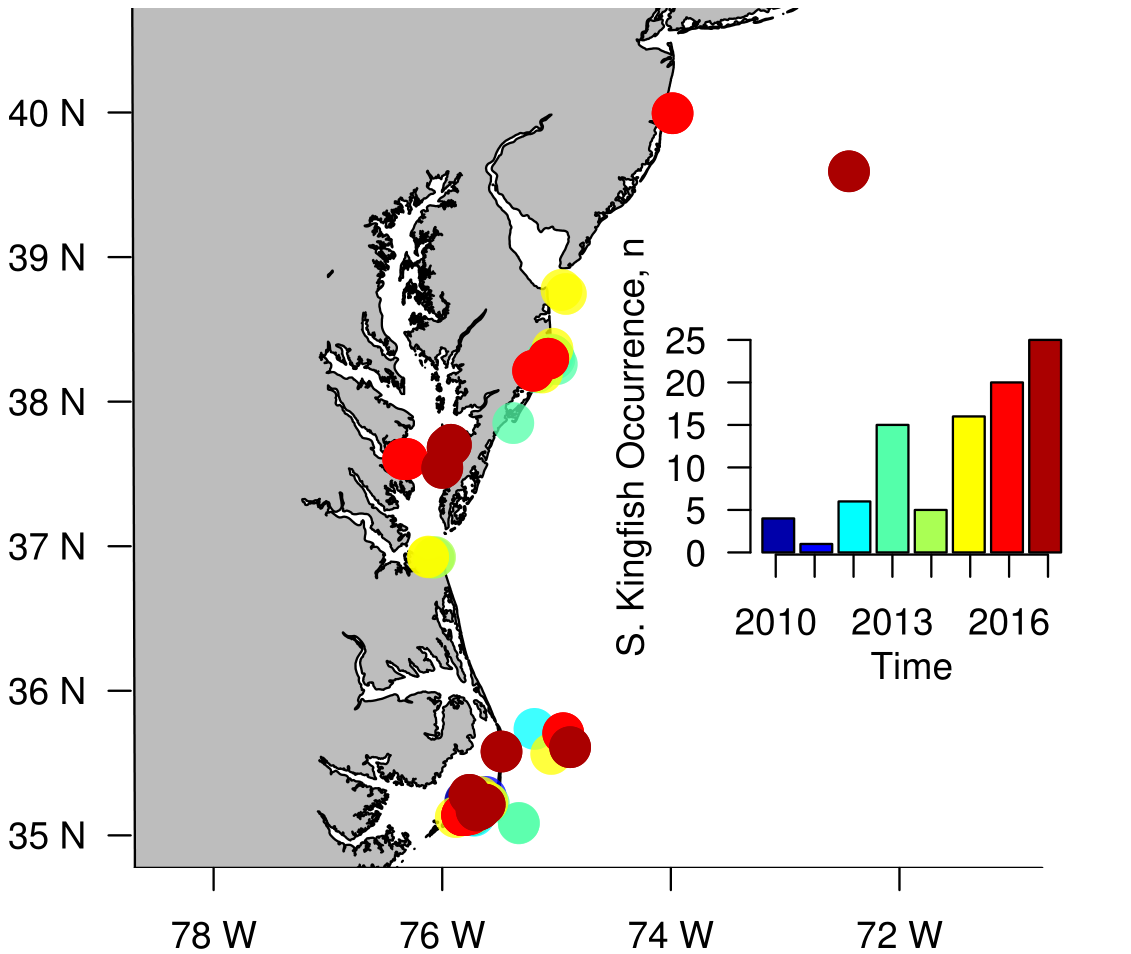
\includegraphics[width=0.8\linewidth]{/home/travis/build/NOAA-EDAB/tech-doc/images/southern_kingfish} 

}

\caption{Verified records of Southern Kingfish occurrence in the Mid-Atlantic.}\label{fig:SK-plot}
\end{figure}

\hypertarget{hab-occu}{%
\chapter{Habitat Occupancy Models}\label{hab-occu}}

\textbf{Description}: Habitat Occupancy

\textbf{Found in}: State of the Ecosystem - Gulf of Maine \& Georges Bank (2018), State of the Ecosystem - Mid-Atlantic (2018)

\textbf{Indicator category}: Database pull with analysis; Extensive analysis; not yet published; Published methods

\textbf{Contributor(s)}: Kevin Friedland

\textbf{Data steward}: Kevin Friedland, \href{mailto:kevin.friedland@noaa.gov}{\nolinkurl{kevin.friedland@noaa.gov}}

\textbf{Point of contact}: Kevin Friedland, \href{mailto:kevin.friedland@noaa.gov}{\nolinkurl{kevin.friedland@noaa.gov}}

\textbf{Public availability statement}: Source data are available upon request (see \protect\hyperlink{survdat}{Survdat}, \protect\hyperlink{chl-pp}{CHL/PP}, and Data Sources below for more information). Model-derived time series are available \href{https://comet.nefsc.noaa.gov/erddap/tabledap/SOE_habitat_soe_v1.html}{here}.

\hypertarget{methods-27}{%
\section{Methods}\label{methods-27}}

Habitat area with a probability of occupancy greater than 0.5 was modeled for many \href{https://www.nefsc.noaa.gov/ecosys/current-conditions/occupancy-change.html}{species throughout the Northeast Large Marine Ecosystem (NE-LME)} using random forest decision tree models.

\hypertarget{data-sources-27}{%
\subsection{Data sources}\label{data-sources-27}}

Models were parameterized using a suite of static and dynamic predictor variables, with occurrence and catch per unit effort (CPUE) of species from spring and fall Northeast Fisheries Science Center (NEFSC) bottom trawl surveys (BTS) serving as response variables. Sources of variables used in the analyses are described below.

\hypertarget{station-depth}{%
\subsubsection{Station depth}\label{station-depth}}

The NEFSC BTS data included depth observations made concurrently with trawls at each station. Station depth was a static variable for these analyses.

\hypertarget{ocean-temperature-and-salinity}{%
\subsubsection{Ocean temperature and salinity}\label{ocean-temperature-and-salinity}}

Sea surface and bottom water temperature and salinity measurements were included as dynamic predictor variables in the model, and were collected using Conductivity/Temperature/Depth (CTD) instruments. Ocean temperature and salinity measurements had the highest temporal coverage during the spring (February-April) and fall (September-November) months. Station salinity data were available between 1992-2016.

\hypertarget{habitat-descriptors}{%
\subsubsection{Habitat descriptors}\label{habitat-descriptors}}

A variety of benthic habitat descriptors were incorporated as predictor variables in occupancy models (Table \ref{tab:habitatdesc}). The majority of these parameters are based on depth (e.g.~\emph{BPI}, \emph{VRM}, \emph{Prcury}, \emph{rugosity}, \emph{seabedforms}, \emph{slp}, and \emph{slpslp}). The vorticity variable is based on current estimates, and the variable \emph{soft\_sed} based on sediment grain size.

\begin{landscape}\begin{table}

\caption{\label{tab:habitatdesc}Habitat descriptors used in model parameterization.}
\centering
\fontsize{8}{10}\selectfont
\begin{tabular}[t]{lll}
\toprule
Variables & Notes & References\\
\midrule
Namera\_vrm & Vector Ruggedness Measure (VRM) measures terrain ruggedness as the variation in three-dimensional orientation of grid cells within a neighborhood based on The Nature Conservancy Northwest Atlantic Marine Ecoregional Assessment ("NAMERA") data. & @Hobson1972; @Sappington2007\\
Prcurv (2 km, 10 km, and 20 km) & Benthic profile curvature at 2km, 10km and 20 km spatial scales was derived from depth data. & @Winship2018\\
Rugosity & A measure of small-scale variations of amplitude in the height of a surface, the ratio of the real to the geometric surface area. & @Friedman2012\\
seabedforms & Seabed topography as measured by a combination of seabed position and slope. & [http://www.northeastoceandata.org/](http://www.northeastoceandata.org/)\\
Slp (2 km, 10 km, and 20 km) & Benthic slope at 2km, 10km and 20km spatial scales. & @Winship2018\\
\addlinespace
Slpslp (2 km, 10 km, and 20 km) & Benthic slope of slope at 2km, 10km and 20km spatial scales & @Winship2018\\
soft\_sed & Soft-sediments is based on grain size distribution from the USGS usSeabed: Atlantic coast offshore surficial sediment data. & [http://www.northeastoceandata.org/](http://www.northeastoceandata.org/)\\
Vort (fall - fa; spring - sp; summer - su; winter - wi) & Benthic current vorticity at a 1/6 degree (approx. 19 km) spatial scale. & @Kinlan2016\\
\bottomrule
\end{tabular}
\end{table}
\end{landscape}

\hypertarget{zooplankton}{%
\subsubsection{Zooplankton}\label{zooplankton}}

Zooplankton data are acquired through the NEFSC Ecosystem Monitoring Program (``EcoMon''). For more information regarding the collection process for these data, see Kane (\protect\hyperlink{ref-Kane2007}{2007}), Kane (\protect\hyperlink{ref-Kane2011}{2011}), and Morse et al. (\protect\hyperlink{ref-Morse2017}{2017}). The bio-volume of the 18 most abundant zooplankton taxa were considered as potential predictor variables.

\hypertarget{remote-sensing-data}{%
\subsubsection{Remote sensing data}\label{remote-sensing-data}}

Both chlorophyll concentration and sea surface temperature (SST) from remote sensing sources were incorporated as static predictor variables in the model. During the period of 1997-2016, chlorophyll concentrations were derived from observations made by the Sea-viewing Wide Field of View Sensor (SeaWIFS), Moderate Resolution Imaging Spectroradiometer (MODIS-Aqua), Medium Resolution Imaging Spectrometer (MERIS), and Visible and Infrared Imaging/Radiometer Suite (VIIRS).

\hypertarget{data-processing-18}{%
\subsection{Data processing}\label{data-processing-18}}

\hypertarget{zooplankton-1}{%
\subsubsection{Zooplankton}\label{zooplankton-1}}

Missing values in the EcoMon time series were addressed by summing data over five-year time steps for each seasonal time frame and interpolating a complete field using ordinary kriging. Missing values necessitated interpolation for spring data in 1989, 1990, 1991, and 1994. The same was true of the fall data for 1989, 1990, and 1992.

\hypertarget{remote-sensing-data-1}{%
\subsubsection{Remote sensing data}\label{remote-sensing-data-1}}

An overlapping time series of observations from the four sensors listed above was created using a bio-optical model inversion algorithm (Maritorena et al. \protect\hyperlink{ref-Maritorena2010}{2010}). Monthly SST data were derived from MODIS-Terra sensor data (available \href{https://oceancolor.gsfc.nasa.gov/data/terra/}{here}).

\hypertarget{ocean-temperature-and-salinity-1}{%
\subsubsection{Ocean temperature and salinity}\label{ocean-temperature-and-salinity-1}}

Date of collection corrections for ocean temperature data were developed using linear regressions for the spring and fall time frames; standardizing to collection dates of April 3 and October 11 for spring and fall. No correction was performed for salinity data. Annual data for ocean temperature and salinity were combined with climatology by season through an optimal interpolation approach. Specifically, mean bottom temperature or salinity was calculated by year and season on a 0.5° grid across the ecosystem, and data from grid cells with \textgreater80\% temporal coverage were used to calculate a final seasonal mean. Annual seasonal means were then used to calculate combined anomalies for seasonal surface and bottom climatologies.

An annual field was then estimated using raw data observations for a year, season, and depth using universal kriging (Hiemstra et al. \protect\hyperlink{ref-automap}{2008}), with depth included as a covariate (on a standard 0.1° grid). This field was then combined with the climatology anomaly field and adjusted by the annual mean using the variance field from kriging as the basis for a weighted mean between the two. The variance field was divided into quartiles with the lowest quartile assigned a weighting of 4:1 between the annual and climatology values. The optimally interpolated field at these locations was therefore skewed towards the annual data, reflecting their proximity to actual data locations and associated low kriging variance. The highest kriging variance quartile (1:1) reflected less information from the annual field and more from the climatology.

\hypertarget{data-analysis-25}{%
\subsection{Data analysis}\label{data-analysis-25}}

\hypertarget{occupancy-models}{%
\subsubsection{Occupancy models}\label{occupancy-models}}

Prior to fitting the occupancy models, predictor variables were tested for multi-collinearity and removed if found to be correlated. The final model variables were then chosen utilizing a model selection process as shown by Murphy, Evans, and Storfer (\protect\hyperlink{ref-Murphy2010}{2010}) and implemented with the R package \texttt{rfUtilities} (Evans and Murphy \protect\hyperlink{ref-rfUtilities-package}{2018}). Occupancy models were then fit as two-factor classification models (absence as 0 and presence as 1) using the \texttt{randomForest} R package (Liaw and Wiener \protect\hyperlink{ref-randomForest}{2002}).

\hypertarget{selection-criteria-and-variable-importance}{%
\subsubsection{Selection criteria and variable importance}\label{selection-criteria-and-variable-importance}}

The \texttt{irr} R package (Gamer, Lemon, and Singh \protect\hyperlink{ref-irr}{2012}) was used to calculate Area Under the ROC Curve (AUC) and Cohen's Kappa for assessing accuracy of occupancy habitat models. Variable importance was assessed by plotting the occurrence of a variable as a root variable versus the mean minimum node depth for the variable (Paluszynska and Biecek \protect\hyperlink{ref-randomForestExplainer}{2017}), as well as by plotting the Gini index decrease versus accuracy decrease.

\hypertarget{plotting-19}{%
\subsection{Plotting}\label{plotting-19}}

\begin{figure}[H]
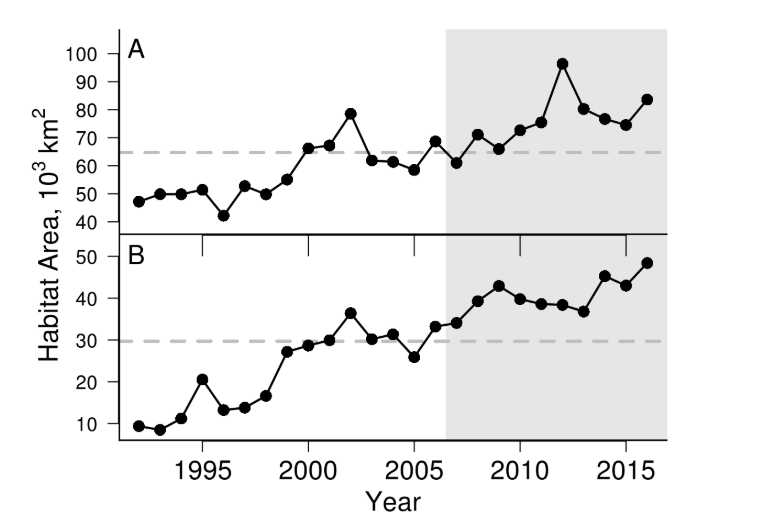
\includegraphics[width=10.78in]{/home/travis/build/NOAA-EDAB/tech-doc/images/habitat_occupancy_plot} \caption{Summer flounder spring (A) and fall (B) occupancy habitat area in the Northeast Large Marine Ecosystem. }\label{fig:occupancy-MAB}
\end{figure}

\hypertarget{primary-production-required}{%
\chapter{Primary Production Required}\label{primary-production-required}}

\textbf{Description}: Time Series of Primary Production Required to sustain reported landings.

\textbf{Found in}: State of the Ecosystem - Gulf of Maine \& Georges Bank (2020+), State of the Ecosystem - Mid-Atlantic (2020+)

\textbf{Indicator category}: Database pull with analysis; Published methods

\textbf{Contributor(s)}: Michael Fogarty, Andrew Beet

\textbf{Data steward}: Andrew Beet, \href{mailto:andrew.beet@noaa.gov}{\nolinkurl{andrew.beet@noaa.gov}}

\textbf{Point of contact}: Andrew Beet, \href{mailto:andrew.beet@noaa.gov}{\nolinkurl{andrew.beet@noaa.gov}}

\textbf{Public availability statement}: Source data is not publicly availabe due to PII restrictions.

\hypertarget{methods-28}{%
\section{Methods}\label{methods-28}}

The index is a measure of the impact of fishing on the base of the foodweb. The amount of potential yield we can expect from a marine ecosystem depends on the amount of production entering at the base of the food web, primarily in the form of phytoplankton; the pathways this energy follows to reach harvested species; the efficiency of transfer of energy at each step in the food web; and the fraction of this production that is removed by the fisheries. Species such as scallops and clams primarily feed directly on larger phytoplankton species and therefore require only one step in the transfer of energy. The loss of energy at each step can exceed 80-90\%. For many fish species, as many as 2-4 steps may be necessary. Given the trophic level and the efficiency of energy transfer of the species in the ecosystem the amount phytoplankton production required (PPR) to account for the observed catch can be estimated.

The index for Primary Production Required (PPR) was adapted from (D Pauly and Christensen \protect\hyperlink{ref-pauly1995ppr}{1995}\protect\hyperlink{ref-pauly1995ppr}{a}).

\[PPR_t = \sum_{i=1}^{n_t}  \left(\frac{landings_{t,i}}{9}\right) \left(\frac{1}{TE}\right)^{TL_i-1}\]

where \(n_t\) = number of species in time \(t\), \(landings_{t,i}\) = landings of species \(i\) in time \(t\), \(TL_i\) is the trophic level of species \(i\), \(TE\) = Trophic efficiency. The PPR estimate assumes a 9:1 ratio for the conversion of wet weight to carbon and a 15\% transfer efficiency per trophic level, (\(TE\) = 0.15)

The index is presented as a percentage of \href{https://noaa-edab.github.io/tech-doc/chl-pp.html}{estimated primary production} (PP) available over the geographic region of interest, termed an \href{https://noaa-edab.github.io/tech-doc/comdat.html}{Ecological Production Unit} (EPU). The scaled index is estimated by dividing the PPR index in year \(t\) by the estimated primary production in time \(t\).

\[scaledPPR_t = \frac{PPR_t}{PP_t}\]

The species selected in each year were determined by their cumulative contribution to total landings. A threshold of at least 80\% of the total landings is used.

\hypertarget{data-sources-28}{%
\subsection{Data sources}\label{data-sources-28}}

Data for this index come from a variety of sources. The landings data come from the Commercial Fishery Database (CFDBS), species trophic level information come from \href{http://fishbase.de}{fishbase} and \href{http://sealifebase.ca}{sealifebase}, and primary production estimates are derived from \href{https://noaa-edab.github.io/tech-doc/chl-pp.html}{satellites}. Some of these data are typically not available to the public.

\hypertarget{data-extraction-24}{%
\subsection{Data extraction}\label{data-extraction-24}}

Landings are extracted from the commercial fisheries database (CFDBS) using the methods described in the chapter \href{https://noaa-edab.github.io/tech-doc/comdat.html}{Commercial Landings Data.}

Trophic level information for each species is obtained from \href{http://fishbase.de}{fishbase} and \href{http://sealifebase.ca}{sealifebase} using the R package \href{https://github.com/ropensci/rfishbase}{rfishbase} (Froese and Pauly \protect\hyperlink{ref-froese2019fishbase}{2019}) in tandem with the package \href{https://github.com/andybeet/indexPPR/}{indexPPR.}

Primary Production is estimated using the methods described in the chapter \href{https://noaa-edab.github.io/tech-doc/chl-pp.html}{Chlorophyll a and Primary Production.}

\hypertarget{data-analysis-26}{%
\subsection{Data analysis}\label{data-analysis-26}}

Annual (wet weight) landings are calculated for each species for a given EPU. For each year the landings are sorted in descending order by species and the cumulative landings are calculated. The top species that accounted for 80\% of total cumulative landings are selected. The trophic level for each of these species are then obtained from fishbase/sealifebase. At this point the PPR index is calculated. The units of the index
are \(gCyear^{-1}\) for the EPU. The index is converted to \(gCm^{-2}year^{-1}\) by dividing by the area (in \(m^2\)) of the EPU.

To normalize the index the total Primiary Production for the given EPU is required. This is calculated as described in the chapter \href{https://noaa-edab.github.io/tech-doc/chl-pp.html}{Chlorophyll a and Primary Production}. The units are also converted to \(gCm^{-2}year^{-1}\).

The index is then normalized by dividing the index in year t by the total primary production in time \(t\).

\hypertarget{plotting-20}{%
\subsection{Plotting}\label{plotting-20}}

Four plots are produced for each EPU:

\begin{itemize}
\tightlist
\item
  The normalized PPR index (along with the associated landings).
\item
  Total primary production
\item
  Mean trophic level of the species included in the index (weighted by their landings)
\item
  Species composition of landings
\end{itemize}

All created using the \href{https://github.com/andybeet/indexPPR}{indexPPR}

See the \href{https://github.com/andybeet/indexPPR/tree/master/vignettes}{workedExample vignette} in the \href{https://github.com/andybeet/indexPPR/}{indexPPR} package for plotting code.

Figures for Mid-Atlantic Bight are presented in this document. For Georges Bank and the Gulf of Maine, please visit \href{(https://github.com/andybeet/indexPPR/tree/master/vignettes/figures)}{here}

\hypertarget{mid-atlantic-bight-mab}{%
\subsubsection{Mid-Atlantic Bight (MAB)}\label{mid-atlantic-bight-mab}}

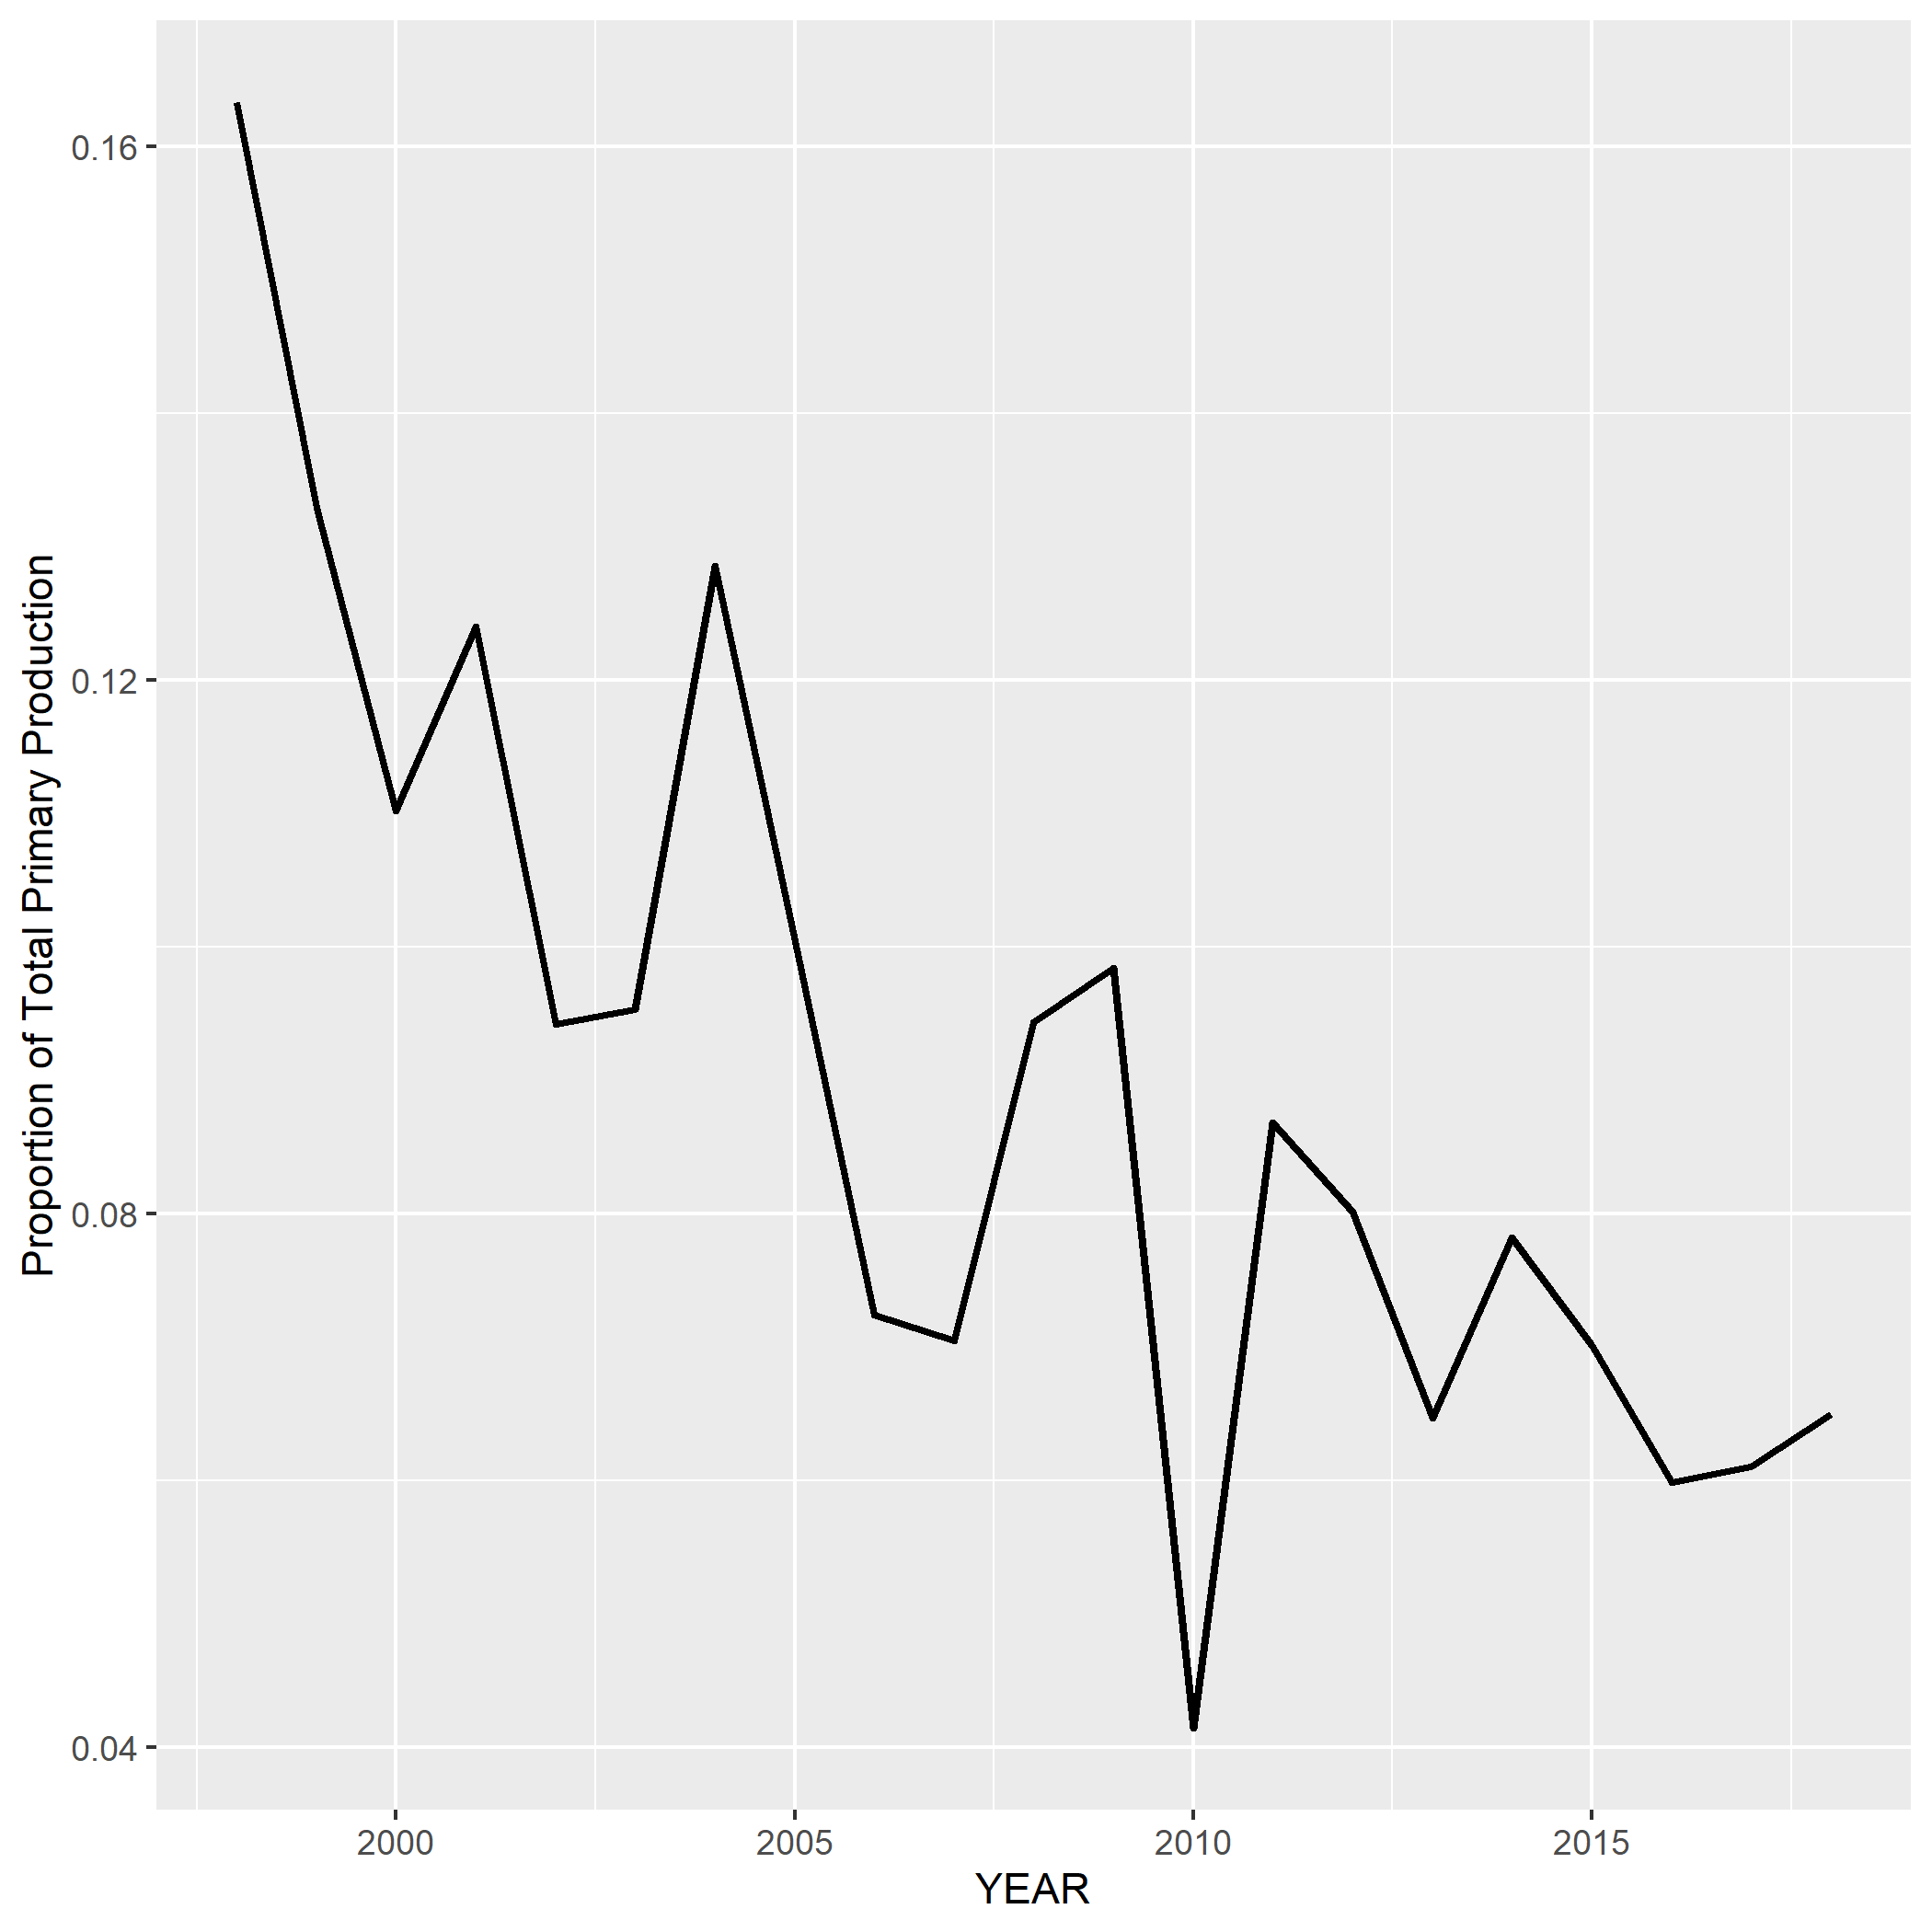
\includegraphics[width=0.5\linewidth]{/home/travis/build/NOAA-EDAB/tech-doc/images/PPR-MAB-0_80}
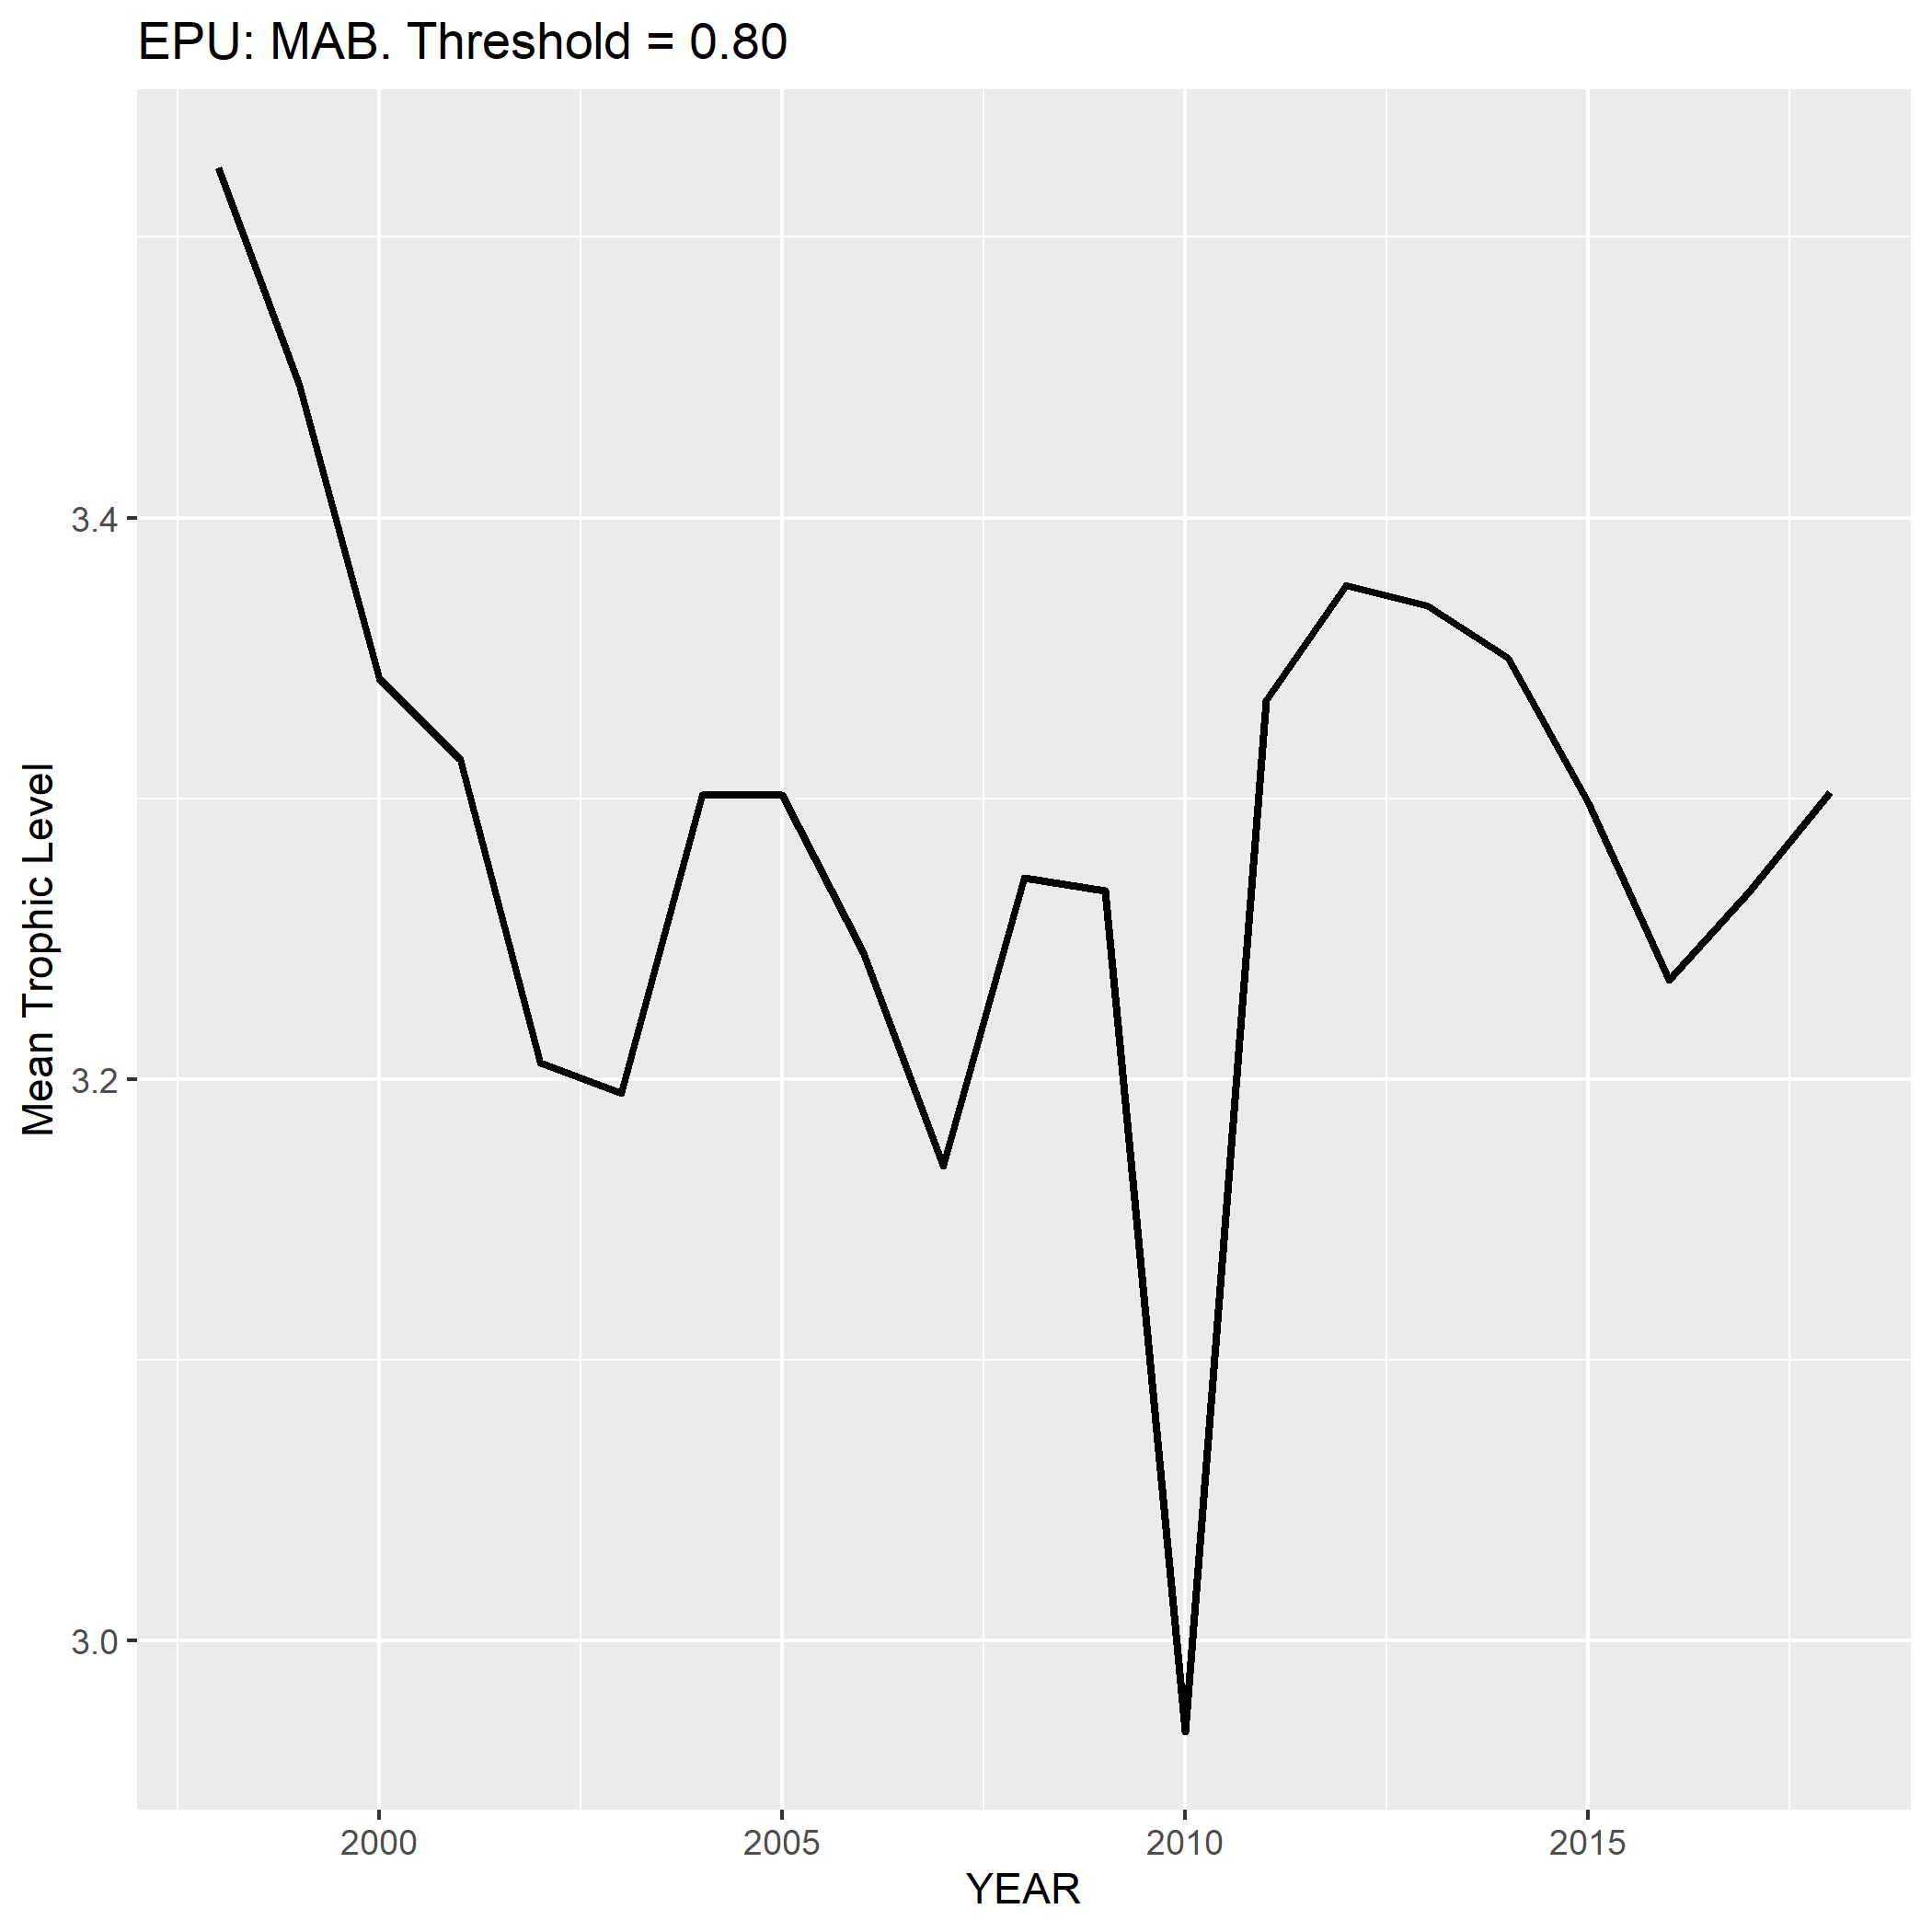
\includegraphics[width=0.5\linewidth]{/home/travis/build/NOAA-EDAB/tech-doc/images/MTL-MAB-0_80}
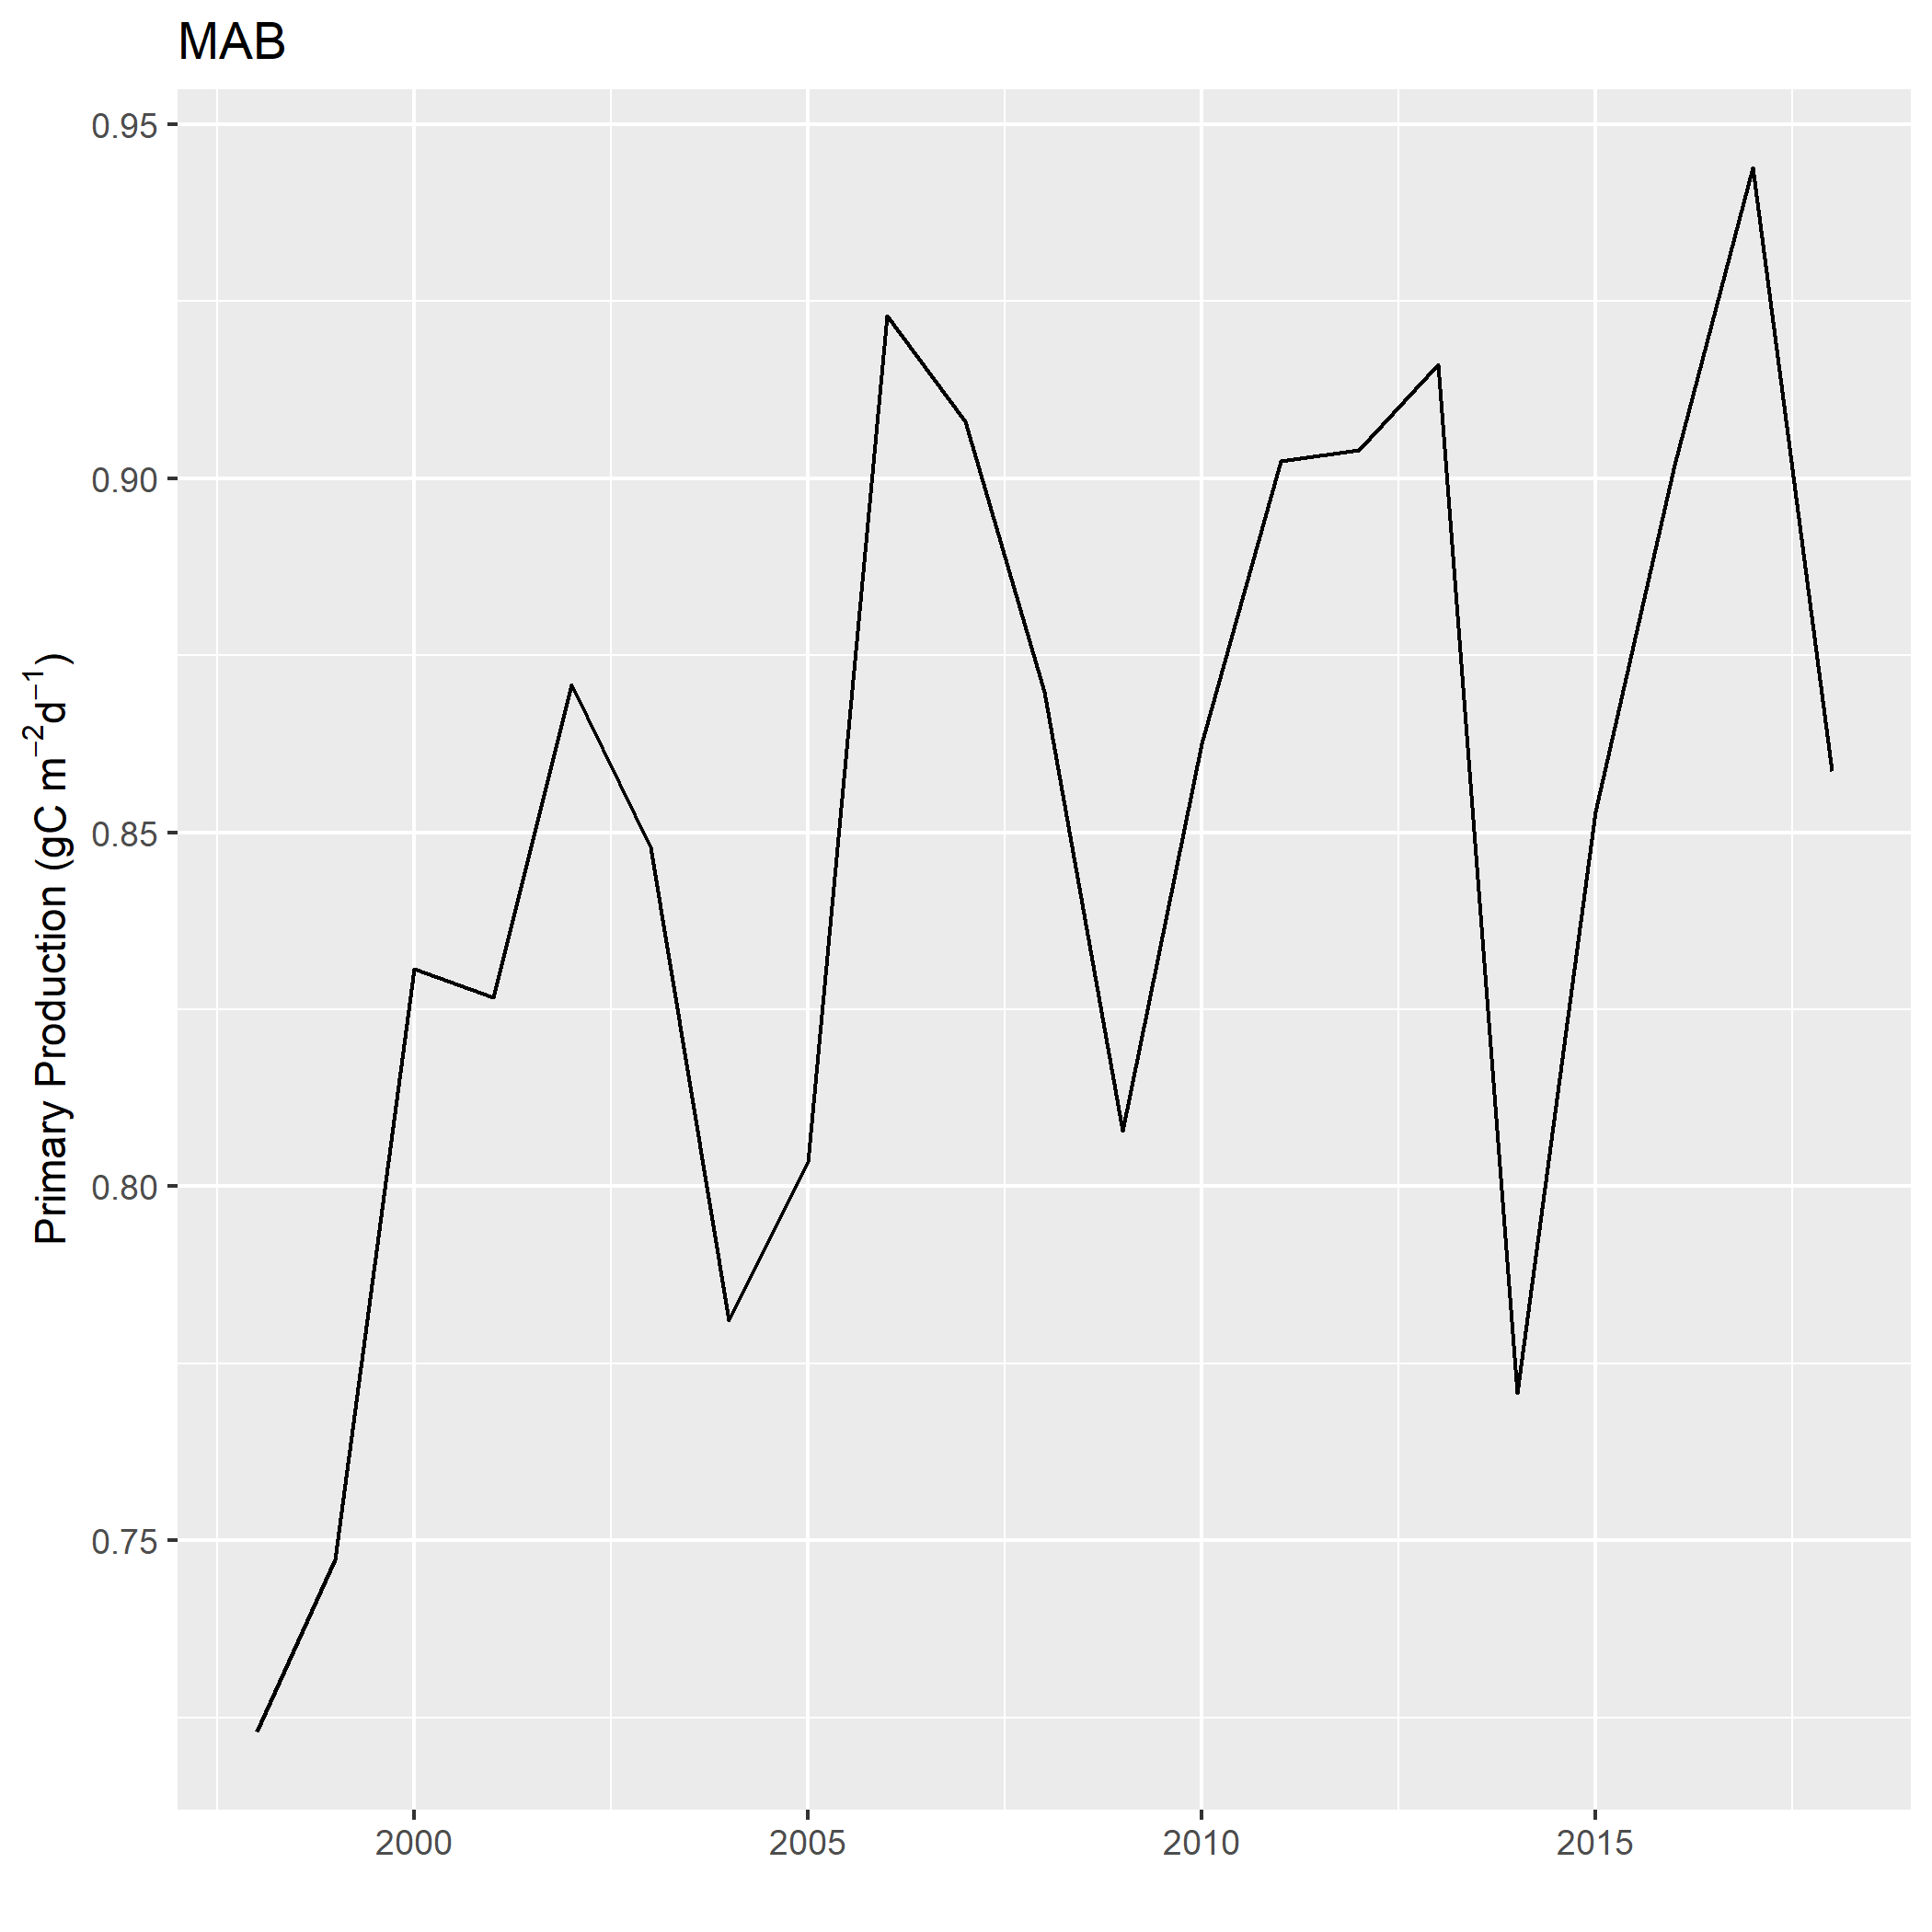
\includegraphics[width=0.5\linewidth]{/home/travis/build/NOAA-EDAB/tech-doc/images/PP-MAB}
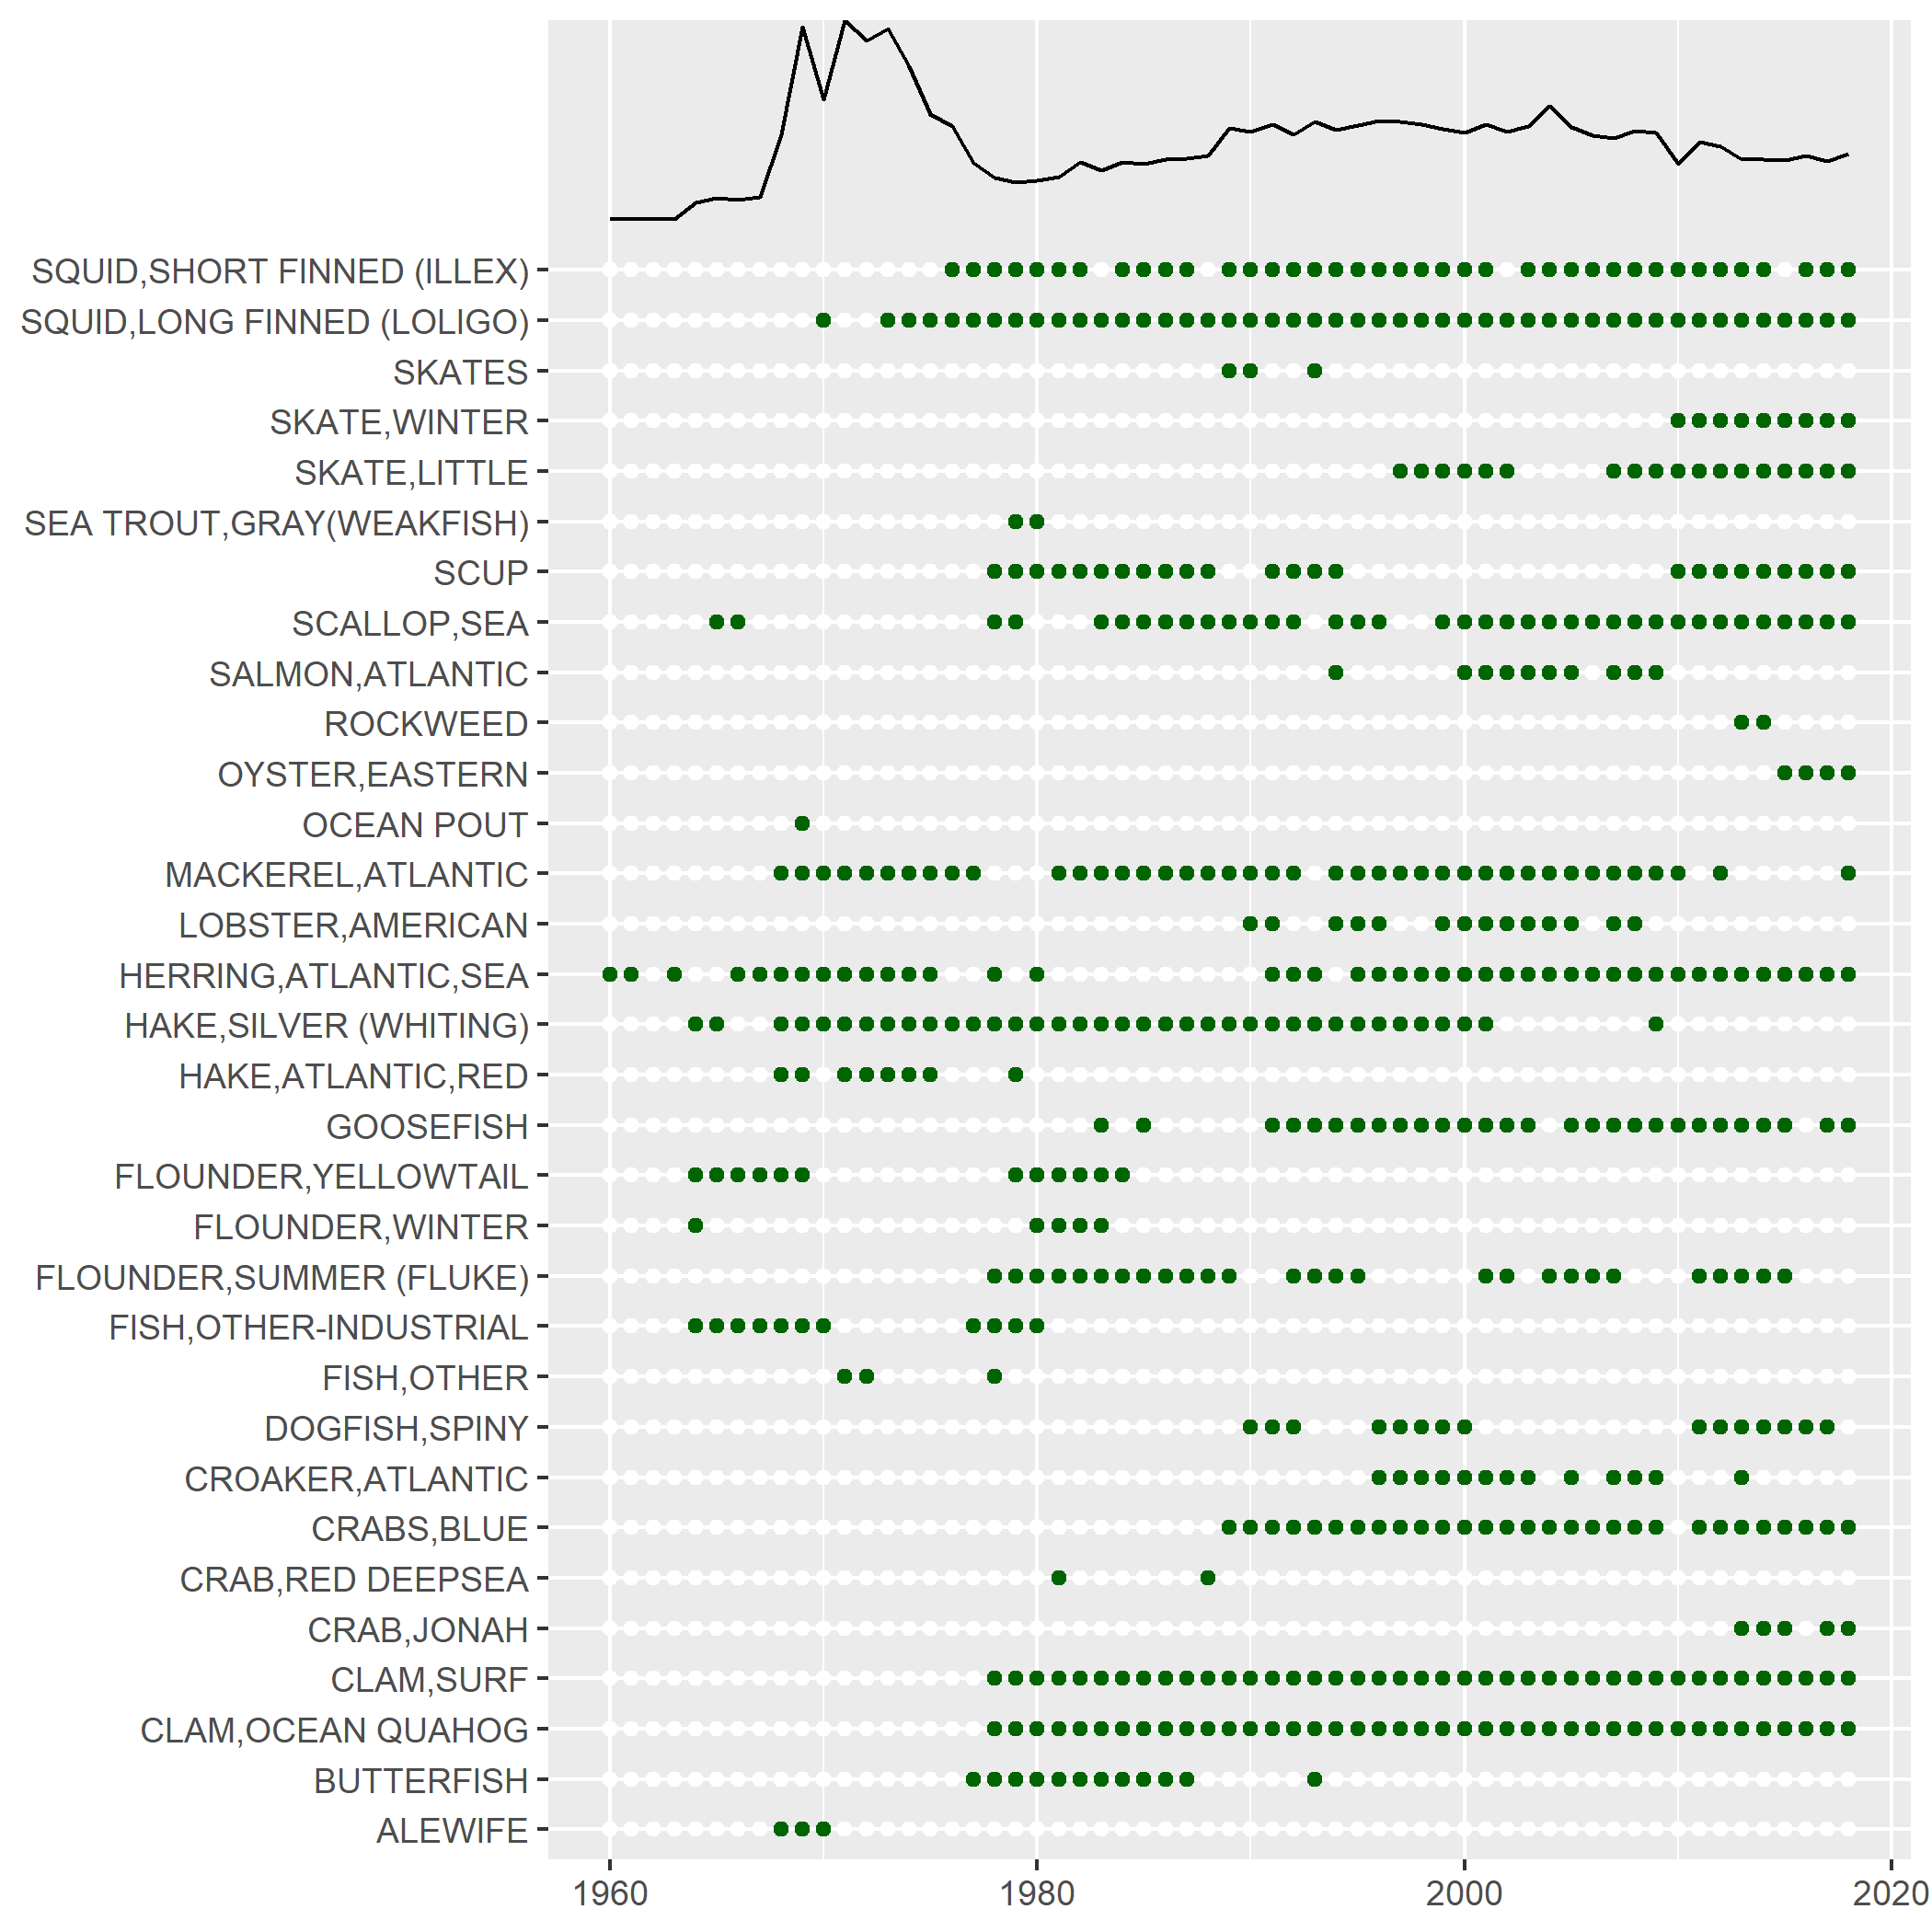
\includegraphics[width=0.5\linewidth]{/home/travis/build/NOAA-EDAB/tech-doc/images/composition-MAB-0_80}

\hypertarget{fish-productivity-indicator}{%
\chapter{Fish Productivity Indicator}\label{fish-productivity-indicator}}

\textbf{Description}: Groundfish productivity estimated as the ratio of small fish to large fish

\textbf{Found in}: State of the Ecosystem - Gulf of Maine \& Georges Bank (2017, 2018, 2020), State of the Ecosystem - Mid-Atlantic (2017, 2018, 2019, 2020)

\textbf{Indicator category}: Database pull with analysis; Published methods

\textbf{Contributor(s)}: Charles Perretti

\textbf{Data steward}: Charles Perretti, \href{mailto:charles.perretti@noaa.gov}{\nolinkurl{charles.perretti@noaa.gov}}

\textbf{Point of contact}: Charles Perretti, \href{mailto:charles.perretti@noaa.gov}{\nolinkurl{charles.perretti@noaa.gov}}

\textbf{Public availability statement}: Source data are available upon request.

\hypertarget{methods-29}{%
\section{Methods}\label{methods-29}}

\hypertarget{data-sources-29}{%
\subsection{Data sources}\label{data-sources-29}}

Survey data from the Northeast Fisheries Science Center (NEFSC) trawl database. These data in their derived form are available through \protect\hyperlink{survdat}{Survdat}.

\hypertarget{data-extraction-25}{%
\subsection{Data extraction}\label{data-extraction-25}}

Data were extracted from \protect\hyperlink{survdat}{Survdat}.

\hypertarget{data-analysis-27}{%
\subsection{Data analysis}\label{data-analysis-27}}

We defined size thresholds separating small and large fish for each species based on the 20th percentile of the length distribution across all years. This threshold was then used to calculate a small and large fish index (numbers below and above the threshold, respectively) each year. Although the length percentile corresponding to age-1 fish will vary with species, we use the 20th percentile as an approximation. Biomass was calculated using length--weight relationships directly from the survey data. Following Wigley, McBride, and McHugh (\protect\hyperlink{ref-wigley_length-weight_2003}{2003}), the length-weight relationship was modeled as
\[\ln W = \ln a + b \ln L\]
where \(W\) is weight (kg), \(L\) is length (cm), and \(a\) and \(b\) are parameters fit via linear regression. The ratio of small fish numbers of the following year to larger fish biomass in the current year was used as the index of recruitment success. The fall and spring recruitment success anomalies were averaged to provide an annual index of recruitment success.

Further details of methods described in Perretti et al. (\protect\hyperlink{ref-perretti_regime_2017}{2017}\protect\hyperlink{ref-perretti_regime_2017}{a}).

\hypertarget{data-processing-19}{%
\subsection{Data processing}\label{data-processing-19}}

Productivity data were formatted for inclusion in the \texttt{ecodata} R package using the R code found \href{https://github.com/NOAA-EDAB/ecodata/blob/master/data-raw/get_productivity_anomaly.R}{here}.

\hypertarget{plotting-21}{%
\subsection{Plotting}\label{plotting-21}}

\begin{figure}
\centering
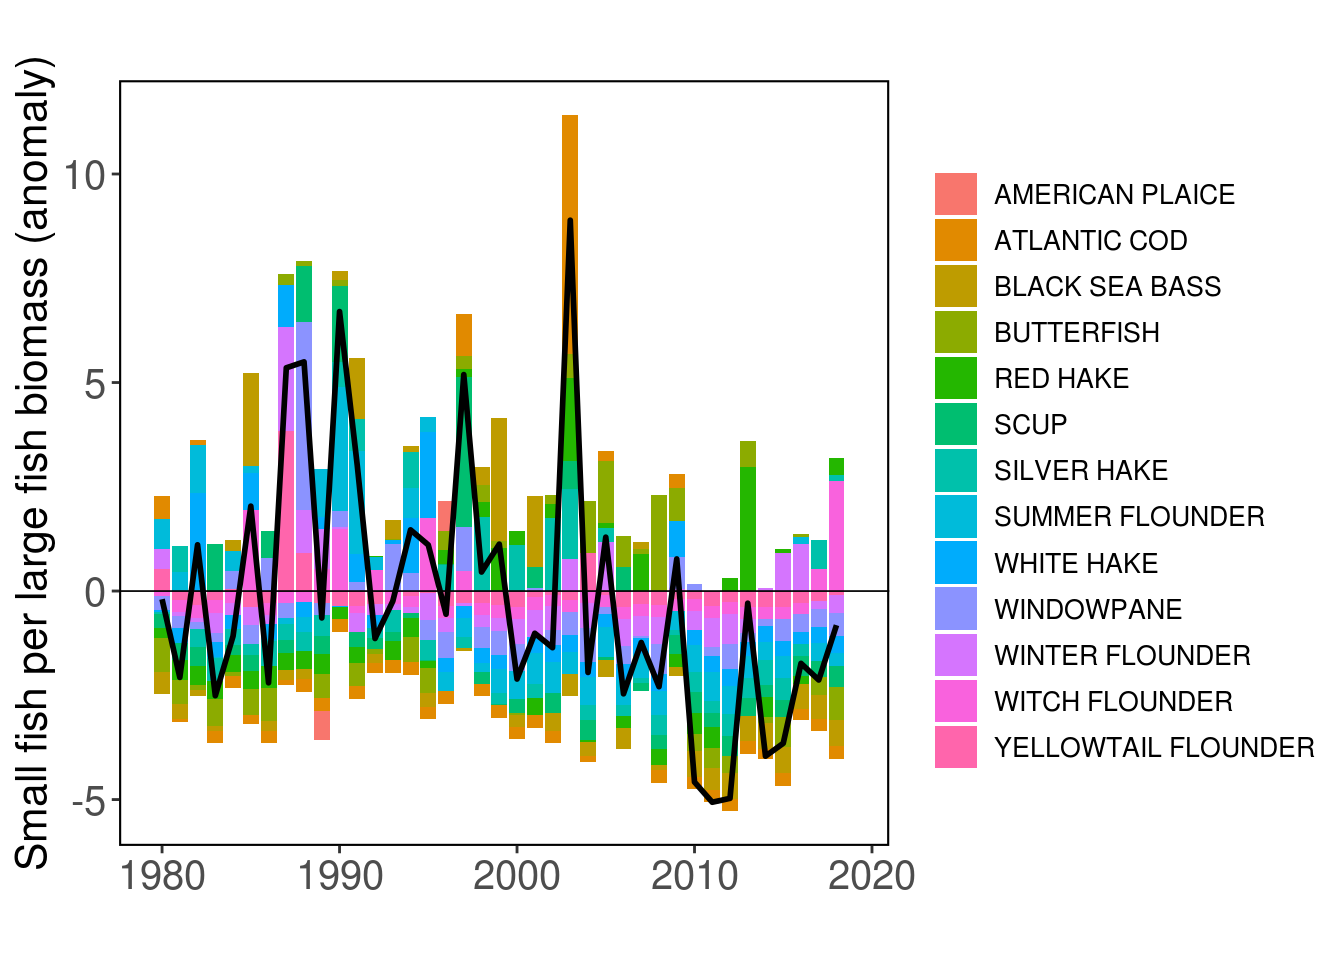
\includegraphics{/home/travis/build/NOAA-EDAB/tech-doc/images/unnamed-chunk-27-1.pdf}
\caption{\label{fig:unnamed-chunk-27}Groundfish productivity across all stocks in the Mid-Atlantic Bight.}
\end{figure}

\hypertarget{recreational-fishing-indicators}{%
\chapter{Recreational Fishing Indicators}\label{recreational-fishing-indicators}}

\textbf{Description}: A variety of indicators derived from MRIP Recreational Fisheries Statistics, including total recreational catch, total angler trips by region, annual diversity of recreational fleet effort, and annual diversity of managed species.

\textbf{Found in}: State of the Ecosystem - Gulf of Maine \& Georges Bank (2017, 2018, 2019, 2020), State of the Ecosystem - Mid-Atlantic (2017, 2018, 2019, 2020)

\textbf{Indicator category}: Database pull with analysis

\textbf{Contributor(s)}: Geret DePiper, Scott Steinbeck

\textbf{Data steward}: Geret DePiper, \href{mailto:geret.depiper@noaa.gov}{\nolinkurl{geret.depiper@noaa.gov}}

\textbf{Point of contact}: Geret DePiper, \href{mailto:geret.depiper@noaa.gov}{\nolinkurl{geret.depiper@noaa.gov}}

\textbf{Public availability statement}: Data sets are publicly available (see Data Sources below).

\hypertarget{methods-30}{%
\section{Methods}\label{methods-30}}

We used total recreational harvest as an indicator of seafood production and total recreational trips and total recreational anglers as proxies for recreational value generated from the Mid-Atlantic and New England regions respectively. We estimated both recreational catch diversity in species manages by the Fisheries Management Councils; Mid-Atlantic (MAFMC), New England (NEFMC) and Atlantic States (ASFMC) and fleet effort diversity using the effective Shannon index.

\hypertarget{data-sources-30}{%
\subsection{Data sources}\label{data-sources-30}}

All recreational fishing indicator data, including number of recreationally harvested fish, number of angler trips, and number of anglers, were downloaded from the Marine Recreational Information Program \href{https://www.st.nmfs.noaa.gov/recreational-fisheries/data-and-documentation/queries/index}{MRIP Recreational Fisheries Statistics Queries} portal. Relevant metadata including information regarding data methodology updates are available at the query site. Note that 2017 data were considered preliminary at the time of the data pull.

Data sets were queried by region on the MRIP site, and for the purposes of the State of the Ecosystem reports, the ``NORTH ATLANTIC'' and ``MID-ATLANTIC'' regions were mapped to the New England and Mid-Atlantic report versions respectively. All query pages are accessible through the \href{https://www.st.nmfs.noaa.gov/recreational-fisheries/data-and-documentation/queries/index}{MRIP Recreational Fisheries Statistics} site.

The number of recreationally harvested fish was found by selecting ``TOTAL HARVEST (A + B1)'' on the \href{https://www.st.nmfs.noaa.gov/recreational-fisheries/data-and-documentation/run-a-data-query}{Catch Time Series Query} page. Catch diversity estimates were also derived from the total catch time series (see below). Species included in the diversity of catch analysis can be found in Table \ref{tab:rec-groups}. The Mid-Atlantic Fishery Management Council asked that species managed by the South Atlantic Fishery Management Council be distinguished in the analysis of recreational species diversity.

\begin{table}

\caption{\label{tab:rec-groups}Species included in recreational catch diversity analysis.}
\centering
\fontsize{8}{10}\selectfont
\begin{tabular}[t]{l|l|l}
\hline
Common.Name & Scientific.Name & Diversity.analysis\\
\hline
American eel & *Anguilla rostrata* & Species inclded in NE and MA analyses\\
\hline
Atlantic Cod & *Gadus morhua* & Species inclded in NE and MA analyses\\
\hline
Atlantic Croacker & *Micropogonias undulatus* & Species inclded in NE and MA analyses\\
\hline
Atlantic Herring & *Clupea harengus* & Species inclded in NE and MA analyses\\
\hline
Atlantic Mackerel & *Scomber scombrus* & Species inclded in NE and MA analyses\\
\hline
Atlantic Menhaden & *Brevoortia tyrannus* & Species inclded in NE and MA analyses\\
\hline
Atlantic Sturgeon & *Acipenser oxyrinchus * & Species inclded in NE and MA analyses\\
\hline
Banded Rudderfish & *Seriola zonata* & Species inclded in NE and MA analyses\\
\hline
Black Sea Bass & *Centropristis striata* & Species inclded in NE and MA analyses\\
\hline
Bluefish & *Pomatomus saltatrix* & Species inclded in NE and MA analyses\\
\hline
Gray Triggerfish & *Balistes capriscus* & Species inclded in NE and MA analyses\\
\hline
Greater Amberjack & *Seriola dumerili* & Species inclded in NE and MA analyses\\
\hline
Little Tunny & *Euthynnus alletteratus * & Species inclded in NE and MA analyses\\
\hline
Pollock & *Pollachius virens* & Species inclded in NE and MA analyses\\
\hline
Rock Sea Bass & *Centropristis philadelphica* & Species inclded in NE and MA analyses\\
\hline
Scup & *Stenotomus chrysops* & Species inclded in NE and MA analyses\\
\hline
Southern Flounder & *Paralichthys lethostigma* & Species inclded in NE and MA analyses\\
\hline
Spiny Dogfish & *Squalus acanthias* & Species inclded in NE and MA analyses\\
\hline
Spot & *Leiostomus xanthurus* & Species inclded in NE and MA analyses\\
\hline
Striped Bass & *Morone saxatilis* & Species inclded in NE and MA analyses\\
\hline
Summer Flounder & *Paralichthys dentatus * & Species inclded in NE and MA analyses\\
\hline
Tautog & *Tautoga onitis* & Species inclded in NE and MA analyses\\
\hline
Tilefish & *Lopholatilus chamaeleonticeps * & Species inclded in NE and MA analyses\\
\hline
Weakfish & *Cynoscion regalis* & Species inclded in NE and MA analyses\\
\hline
Winter Flounder & *Pseudopleuronectes americanus* & Species inclded in NE and MA analyses\\
\hline
Black Drum & *Pogonias cromis* & SAFMC managed species included in MA analysis\\
\hline
Cobia & *Rachycentron canadum* & SAFMC managed species included in MA analysis\\
\hline
Lesser Amberjack & *Seriola fasciata* & SAFMC managed species included in MA analysis\\
\hline
Red Drum & *Sciaenops ocellatus* & SAFMC managed species included in MA analysis\\
\hline
Red Porgy & *Pagrus pagrus * & SAFMC managed species included in MA analysis\\
\hline
Wahoo & *Acanthocybium solandri* & SAFMC managed species included in MA analysis\\
\hline
Bar Jack & *Caranx ruber* & SAFMC managed species included in MA analysis\\
\hline
Blue Runner & *Caranx crysos * & SAFMC managed species included in MA analysis\\
\hline
Hogfish & *Lachnolaimus maximus* & SAFMC managed species included in MA analysis\\
\hline
Jolthead Porgy & *Calamus bajonado* & SAFMC managed species included in MA analysis\\
\hline
Margate & *Haemulon album* & SAFMC managed species included in MA analysis\\
\hline
Almaco Jack & *Seriola rivoliana* & SAFMC managed species included in MA analysis\\
\hline
Atlantic Spadefis & *Chaetodipterus faber * & SAFMC managed species included in MA analysis\\
\hline
Ocean Triggerfish & *Canthidermis sufflamen * & SAFMC managed species included in MA analysis\\
\hline
Spanish Mackerel & *Scomberomorus maculatus* & SAFMC managed species included in MA analysis\\
\hline
Spotted Seatrout & *Cynoscion nebulosus * & SAFMC managed species included in MA analysis\\
\hline
Tomtate & *Haemulon aurolineatum* & SAFMC managed species included in MA analysis\\
\hline
Gray Snapper & *Lutjanus griseus* & SAFMC managed species included in MA analysis\\
\hline
Mutton Snapper & *Lutjanus analis* & SAFMC managed species included in MA analysis\\
\hline
Coney & *Cephalopholis fulva* & SAFMC managed species included in MA analysis\\
\hline
White Grunt & *Haemulon plumierii* & SAFMC managed species included in MA analysis\\
\hline
Yellowtail Snapper & *Ocyurus chrysurus* & SAFMC managed species included in MA analysis\\
\hline
Snowy Grouper & *Hyporthodus niveatus* & SAFMC managed species included in MA analysis\\
\hline
Blueline Tilefish & *Caulolatilus microps* & SAFMC managed species included in MA analysis\\
\hline
Longspine Porgy & *Stenotomus caprinus * & SAFMC managed species included in MA analysis\\
\hline
Wreckfish & *Polyprion americanus* & SAFMC managed species included in MA analysis\\
\hline
Gag & *Mycteroperca microlepis* & SAFMC managed species included in MA analysis\\
\hline
Haddock & *Melanogrammus aeglefinus* & SAFMC managed species included in MA analysis\\
\hline
Whitebone Porgy & *Calamus leucosteus* & SAFMC managed species included in MA analysis\\
\hline
\end{tabular}
\end{table}

Angler trips (listed as ``TOTAL'' trips) were pulled from the MRIP \href{https://www.st.nmfs.noaa.gov/recreational-fisheries/data-and-documentation/run-a-data-query}{Effort Time Series Query} page, and included data from 1981 - 2019. Time series of recreational fleet effort diversity were calculated from this data set (see below). The number of anglers was total number of anglers from the Marine Recreational Fishery Statistics Survey (MRFSS) Participation Time Series Query, and includes data from 1981 - 2016.

\hypertarget{data-analysis-28}{%
\subsection{Data analysis}\label{data-analysis-28}}

\textbf{Recreational fleet effort diversity}

Code used to for effort diversity data analysis can be found \href{https://github.com/NOAA-EDAB/tech-doc/blob/master/R/stored_scripts/rec_effort_div_analysis.R}{here}.

\textbf{Recreational catch diversity}

Code used to for catch diversity data analysis can be found \href{https://github.com/NOAA-EDAB/tech-doc/blob/master/R/stored_scripts/rec_catch_div_analysis.R}{here}.

\hypertarget{data-processing-20}{%
\subsection{Data processing}\label{data-processing-20}}

Recreational fishing indicators were formatted for inclusion in the \texttt{ecodata} R package using this \href{https://github.com/NOAA-EDAB/ecodata/blob/master/data-raw/get_rec.R}{code}.

\hypertarget{plotting-22}{%
\subsection{Plotting}\label{plotting-22}}

\begin{figure}
\centering
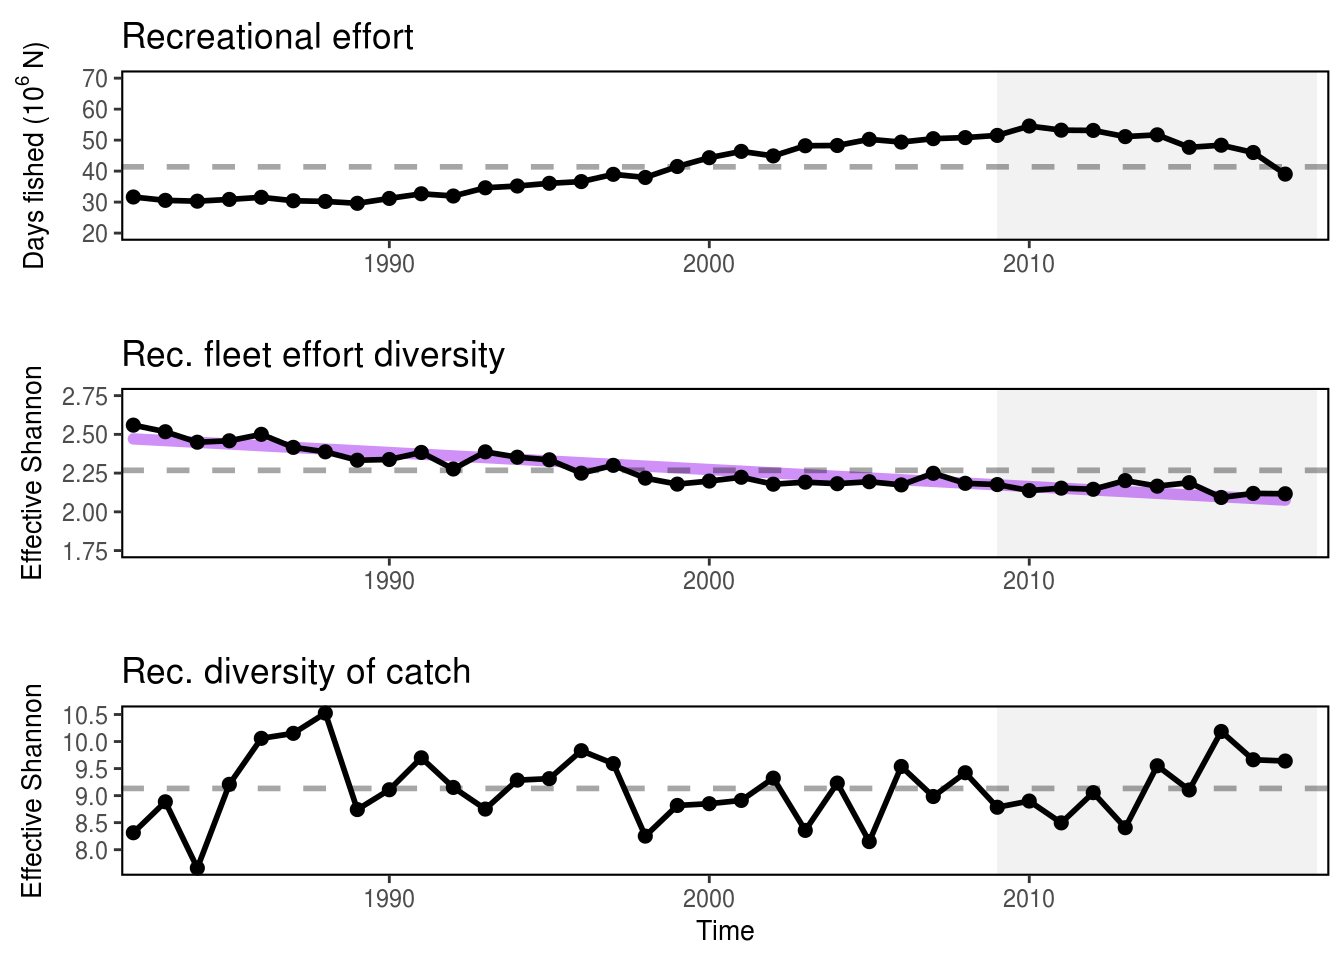
\includegraphics{/home/travis/build/NOAA-EDAB/tech-doc/images/unnamed-chunk-28-1.pdf}
\caption{\label{fig:unnamed-chunk-28}Recreational effort diversity and diversity of recreational catch in the Mid-Atlantic.}
\end{figure}

\begin{figure}
\centering
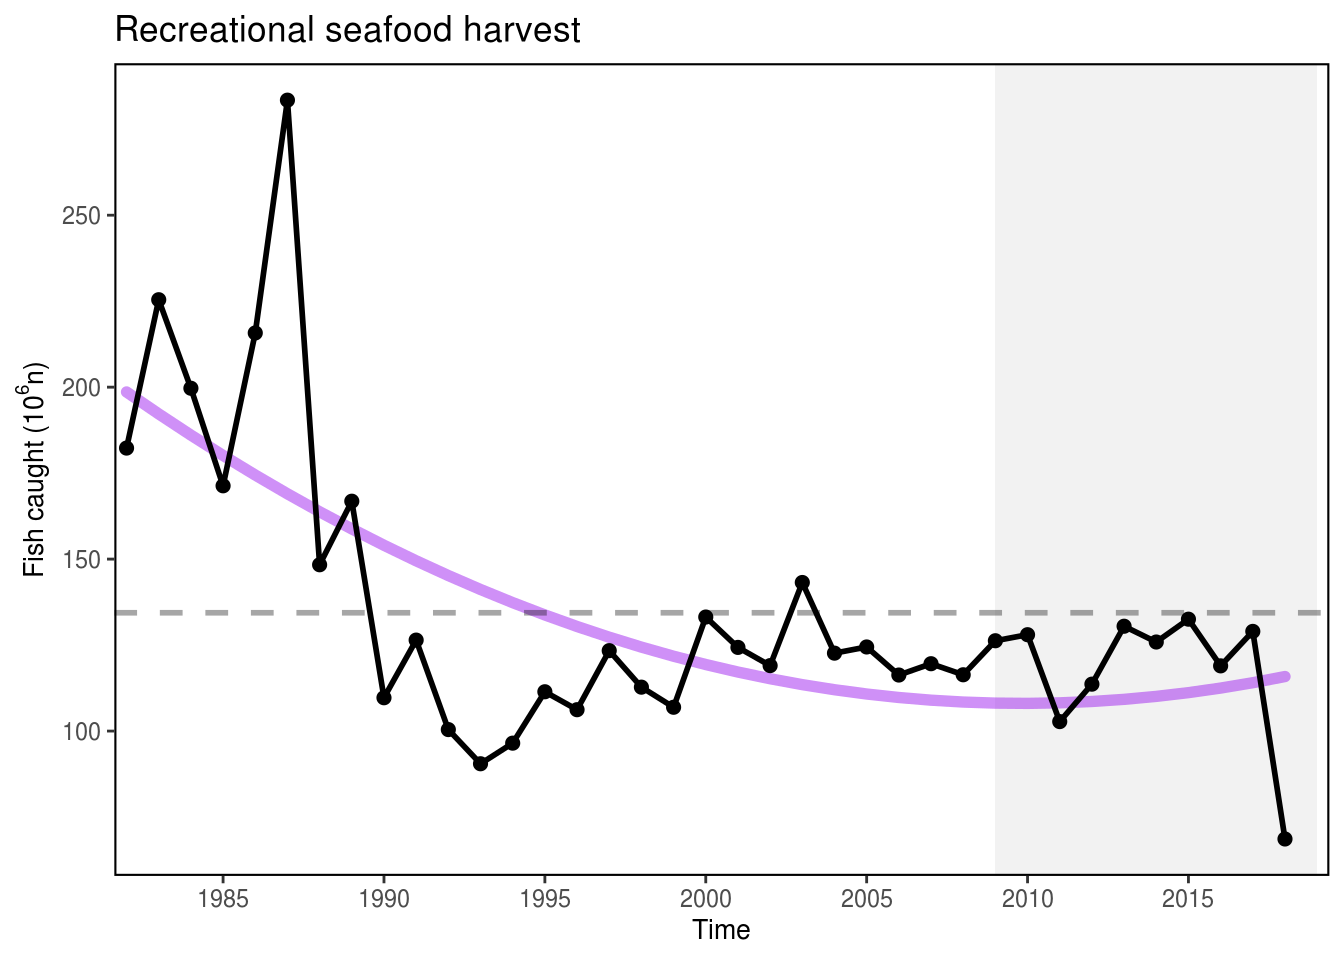
\includegraphics{/home/travis/build/NOAA-EDAB/tech-doc/images/unnamed-chunk-29-1.pdf}
\caption{\label{fig:unnamed-chunk-29}Total recreational seafood harvest in the Mid-Atlantic.}
\end{figure}

\hypertarget{right-whale-abundance}{%
\chapter{Right Whale Abundance}\label{right-whale-abundance}}

\textbf{Description}: Right Whale

\textbf{Found in}: State of the Ecosystem - Gulf of Maine \& Georges Bank (2017, 2018, 2019, 2020), State of the Ecosystem - Mid-Atlantic (2017, 2018, 2019, 2020)

\textbf{Indicator category}: Synthesis of published information; Published methods

\textbf{Contributor(s)}: Christopher D. Orphanides

\textbf{Data steward}: Chris Orphanides, \href{mailto:chris.orphanides@noaa.gov}{\nolinkurl{chris.orphanides@noaa.gov}}

\textbf{Point of contact}: Richard Pace, \href{mailto:richard.pace@noaa.gov}{\nolinkurl{richard.pace@noaa.gov}}

\textbf{Public availability statement}: Source data are available from the New England Aquarium upon request. Derived data are available \href{http://comet.nefsc.noaa.gov/erddap/tabledap/protected_species_soe_v1.html}{here}

\hypertarget{methods-31}{%
\section{Methods}\label{methods-31}}

\hypertarget{data-sources-31}{%
\subsection{Data sources}\label{data-sources-31}}

The North Atlantic right whale abundance estimates were taken from a published document (see Pace, Corkeron, and Kraus \protect\hyperlink{ref-Pace2017}{2017}), except for the most recent 2016 and 2017 estimates. Abundance estimates from 2016 and 2017 were taken from the 2016 National Oceanographic and Atmospheric Administration marine mammal stock assessment (Hayes et al. \protect\hyperlink{ref-Hayes2017}{2017}) and an unpublished 2017 stock assessment.

Calves birth estimates are taken from a published report (Pettis, Pace, and Hamilton \protect\hyperlink{ref-narw2019}{2019}) put out yearly by the North American Right Whale Consortium.

\hypertarget{data-extraction-26}{%
\subsection{Data extraction}\label{data-extraction-26}}

Data were collected from existing reports and validated by report authors.

\hypertarget{data-analysis-29}{%
\subsection{Data analysis}\label{data-analysis-29}}

Analysis for right whale abundance estimates is provided by Pace, Corkeron, and Kraus (\protect\hyperlink{ref-Pace2017}{2017}), and code can be found in the \href{https://onlinelibrary.wiley.com/action/downloadSupplement?doi=10.1002\%2Fece3.3406\&file=ece33406-sup-0001-SupInfo.docx}{supplemental materials}.

\hypertarget{data-processing-21}{%
\subsection{Data processing}\label{data-processing-21}}

Time series of right whale and calf abundance estimates were formatted for inclusion in the \texttt{ecodata} R package using this R \href{https://github.com/NOAA-EDAB/ecodata/blob/master/data-raw/get_narw.R}{code}.

\hypertarget{plotting-23}{%
\subsection{Plotting}\label{plotting-23}}

Code used create the plots below can be found at these links, NARW \href{https://github.com/NOAA-EDAB/ecodata/blob/master/chunk-scripts/macrofauna.Rmd-NARW-abundance.R}{population estimates} and \href{https://github.com/NOAA-EDAB/ecodata/blob/master/chunk-scripts/macrofauna.Rmd-NARW-calf-abundance.R}{calf births}.

\begin{figure}
\centering
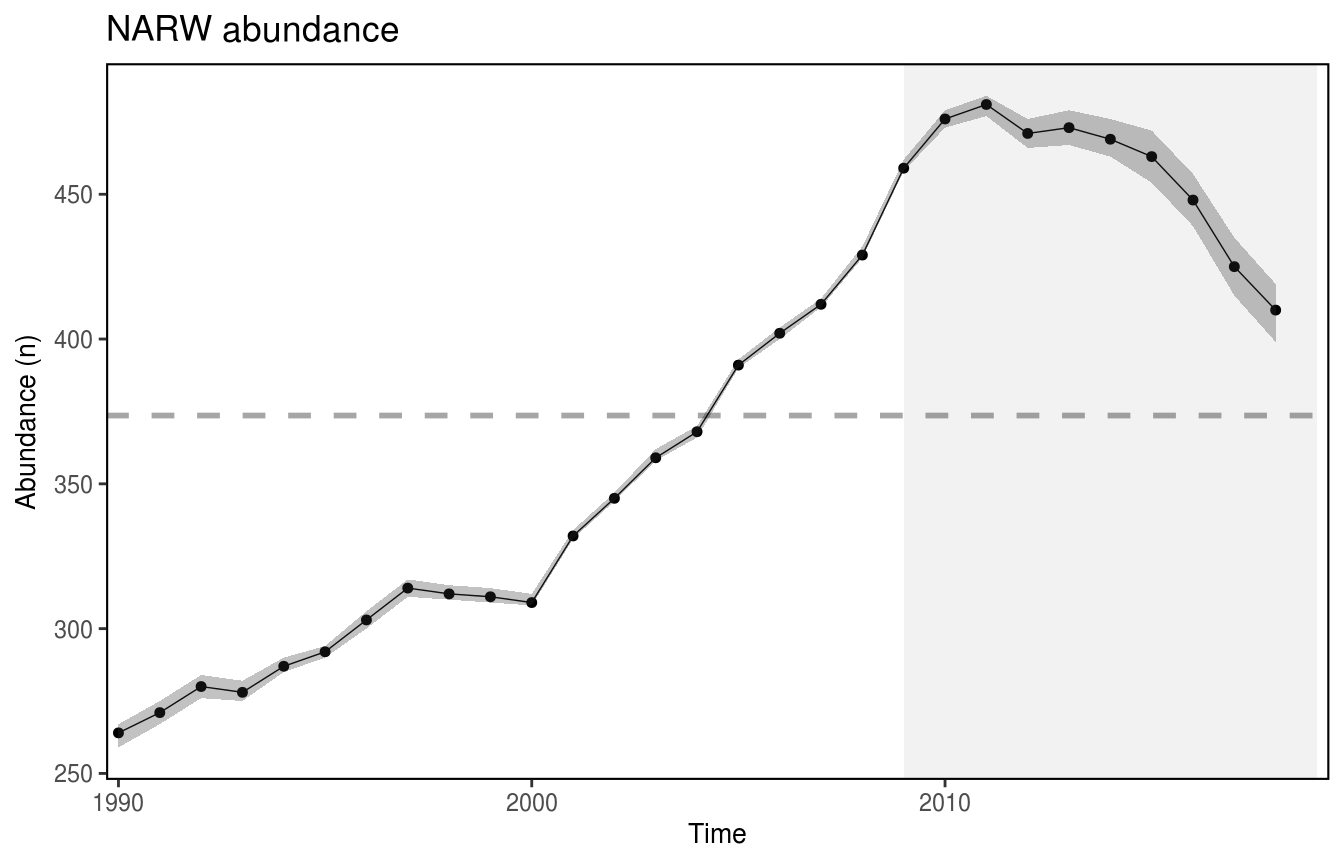
\includegraphics{/home/travis/build/NOAA-EDAB/tech-doc/images/unnamed-chunk-31-1.pdf}
\caption{\label{fig:unnamed-chunk-31}North Atlantic right whale population estimates shown with 95\% credible intervals.}
\end{figure}

\begin{figure}
\centering
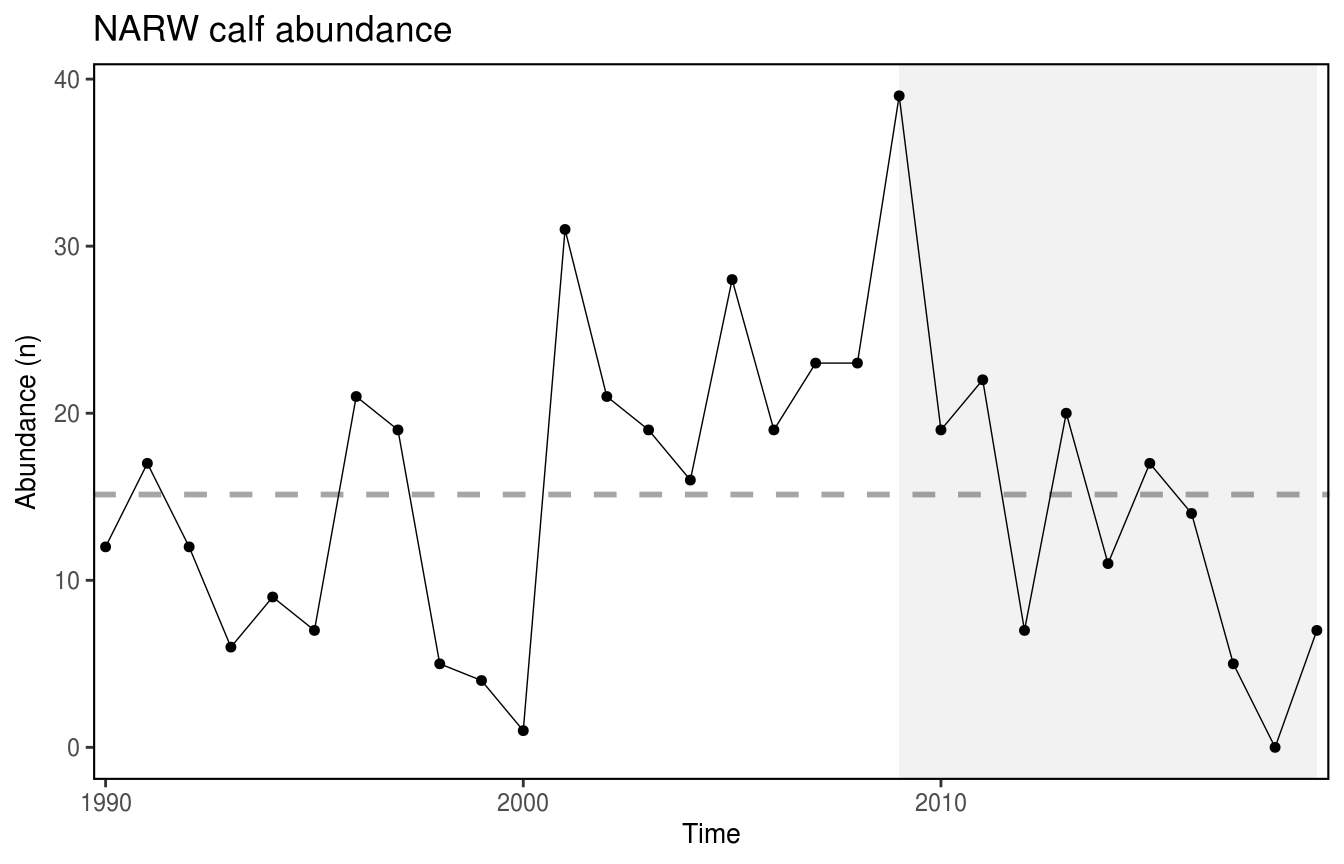
\includegraphics{/home/travis/build/NOAA-EDAB/tech-doc/images/unnamed-chunk-32-1.pdf}
\caption{\label{fig:unnamed-chunk-32}North Atlantic right whale calf births.}
\end{figure}

\hypertarget{safmc-managed-spp}{%
\chapter{SAFMC managed spp}\label{safmc-managed-spp}}

\textbf{Description}: SAFMC Species on NES

\textbf{Found in}: State of the Ecosystem - Mid-Atlantic (2020), State of the Ecosystem - New England (2020)

\textbf{Indicator category}: Database pull

\textbf{Contributor(s)}: Sean Lucey

\textbf{Data steward}: Sean Lucey \href{mailto:Sean.Lucey@noaa.gov}{\nolinkurl{Sean.Lucey@noaa.gov}}

\textbf{Point of contact}: Sean Lucey \href{mailto:Sean.Lucey@noaa.gov}{\nolinkurl{Sean.Lucey@noaa.gov}}

\textbf{Public availability statement}: Source data are available to qualified researchers upon request (see ``Access Information'' \href{https://inport.nmfs.noaa.gov/inport/item/22560}{here}).

\hypertarget{methods-32}{%
\section{Methods}\label{methods-32}}

\hypertarget{data-sources-32}{%
\subsection{Data sources}\label{data-sources-32}}

The \protect\hyperlink{survdat}{Survdat} data set was used to examine the presence of ``southern'' species (table \ref{tab:southern}) in Mid-Atlantic and New England waters.

\hypertarget{data-extraction-27}{%
\subsection{Data extraction}\label{data-extraction-27}}

Survdat was subsetted by common ``southern'' species (table \ref{tab:soe2018class}).

\begin{table}

\caption{\label{tab:southern}Southern Species that were examined within the NEFSC trawl survey data}
\centering
\begin{tabular}[t]{l>{\em}ll}
\toprule
Common.Name & Scientific.Name & Group\\
\midrule
Black snapper & Apsilus dentatus & Snappers\\
Queen snapper & Etelis oculatus & Snappers\\
Mutton snapper & Lutjanus analis & Snappers\\
Schoolmaster snapper & Lutjanus apodus & Snappers\\
Blackfin snapper & Lutjanus buccanella & Snappers\\
\addlinespace
Northern Red snapper & Lutjanus campechanus & Snappers\\
Cubera snapper & Lutjanus cyanopterus & Snappers\\
Grey snapper & Lutjanus griseus & Snappers\\
Mahogany snapper & Lutjanus mahogoni & Snappers\\
Dog snapper & Lutjanus jocu & Snappers\\
\addlinespace
Lane snapper & Lutjanus synagris & Snappers\\
Silk snapper & Lutjanus vivanus & Snappers\\
Yellowtail snapper & Ocyurus chrysurus & Snappers\\
Vermilion snapper & Rhomboplites aurorubens & Snappers\\
Bank sea bass & Centropristis ocyurus & Sea Basses\\
\addlinespace
Rock sea bass & Centropristis philadelphica & Sea Basses\\
Black sea bass & Centropristis striata & Sea Basses\\
Rock hind & Epinephelus adscensionis & Groupers\\
Graysby & Epinephelus cruentatus & Groupers\\
Calico grouper & Epinephelus drummondhayi & Groupers\\
\addlinespace
Yellowedge grouper & Epinephelus flavolimbatus & Groupers\\
Coney & Epinephelus fulvus & Groupers\\
Red hind & Epinephelus guttatus & Groupers\\
Atlantic goliath grouper & Epinephelus itajara & Groupers\\
Red grouper & Epinephelus mario & Groupers\\
\addlinespace
Misty grouper & Epinephelus mystacinus & Groupers\\
Warsaw grouper & Epinephelus nigritus & Groupers\\
Snowy grouper & Epinephelus niveatus & Groupers\\
Nassau grouper & Epinephelus striatus & Groupers\\
Black grouper & Mycteroperca bonaci & Groupers\\
\addlinespace
Yellowmouth grouper & Mycteroperca interstitialis & Groupers\\
Gag grouper & Mycteroperco microlepis & Groupers\\
Scamp grouper & Mycteroperca phenax & Groupers\\
Tiger grouper & Mycteroperca tigris & Groupers\\
Yellowfin grouper & Mycteroperca venenoso & Groupers\\
\addlinespace
Sheepshead & Archosargus probotocephalus & Porgies\\
Grass porgy & Calamus arctifrons & Porgies\\
Jolthead porgy & Calamus bajonado & Porgies\\
Saucereye porgy & Calamus calamus & Porgies\\
Whitebone porgy & Calamus leucosteus & Porgies\\
\addlinespace
Knobbed porgy & Calamus leucosteus & Porgies\\
Red porgy & Pagrus pagrus & Porgies\\
Longspine porgy & Stenotomus caprinus & Porgies\\
Black margate & Anisotremus surinamensis & Grunts\\
Porkfish & Anisotremus virginicus & Grunts\\
\addlinespace
White margate & Haemulon album & Grunts\\
Tomtate & Haemulon aurolineatum & Grunts\\
Smallmouth grunt & Hemulon chrysargyreum & Grunts\\
French grunt & Haemulon flavolineatum & Grunts\\
Spanish grunt & Haemulon macrostomum & Grunts\\
\addlinespace
Cottonwick grunt & Haemulon melanurum & Grunts\\
Sailor's grunt & Haemulon parra & Grunts\\
White grunt & Haemulon plumieri & Grunts\\
Blue Striped grunt & Haemulon sciurus & Grunts\\
Grey triggerfish & Balistes capriscus & Triggerfishes\\
\addlinespace
Queen triggerfish & Balistes vetula & Triggerfishes\\
Ocean triggerfish & Canthidermis sufflamen & Triggerfishes\\
Hogfish & Lachnolaimus maximus & Wrasses\\
Puddingwife wrasse & Halichoeres rodiatus & Wrasses\\
Yellow jack & Caranx bartholomaei & Jacks\\
\addlinespace
Blue runner & Caranx crysos & Jacks\\
Crevalle jack & Caranx hippos & Jacks\\
Bar jack & Caranx ruber & Jacks\\
Greater amberjack & Seriola dumerili & Jacks\\
Almaco jack & Seriola rivoliano & Jacks\\
\bottomrule
\end{tabular}
\end{table}

\hypertarget{data-analysis-30}{%
\subsection{Data analysis}\label{data-analysis-30}}

The presence/absence of ``southern'' species was broadly examined for all species listed in table \ref{tab:southern}. It was quickly determined that these species were extremely rare in the bottom trawl survey. When a species was present, they were found during the fall survey and not the spring. No trends were apparent in the data. The one species that was commonly present was the blue runner (\emph{Caranx crysos}). Stations were binned temporally by three categories: Prior to 2001, 2001 - 2010, and since 2010. Stations were then plotted on a map of the survey region and visually inspected.

\hypertarget{data-processing-22}{%
\subsection{Data processing}\label{data-processing-22}}

Blue runner (\emph{Caranx crysos}) data were formatted for inclusion in the \texttt{ecodata} R package using this \href{https://github.com/NOAA-EDAB/ecodata/blob/master/data-raw/get_blue_runner.R}{R code}.

\hypertarget{plotting-24}{%
\subsection{Plotting}\label{plotting-24}}

The plot below was built using the code found
\href{https://github.com/NOAA-EDAB/ecodata/blob/master/chunk-scripts/macrofauna.Rmd-blue-runner.R}{here}.

\begin{figure}
\centering
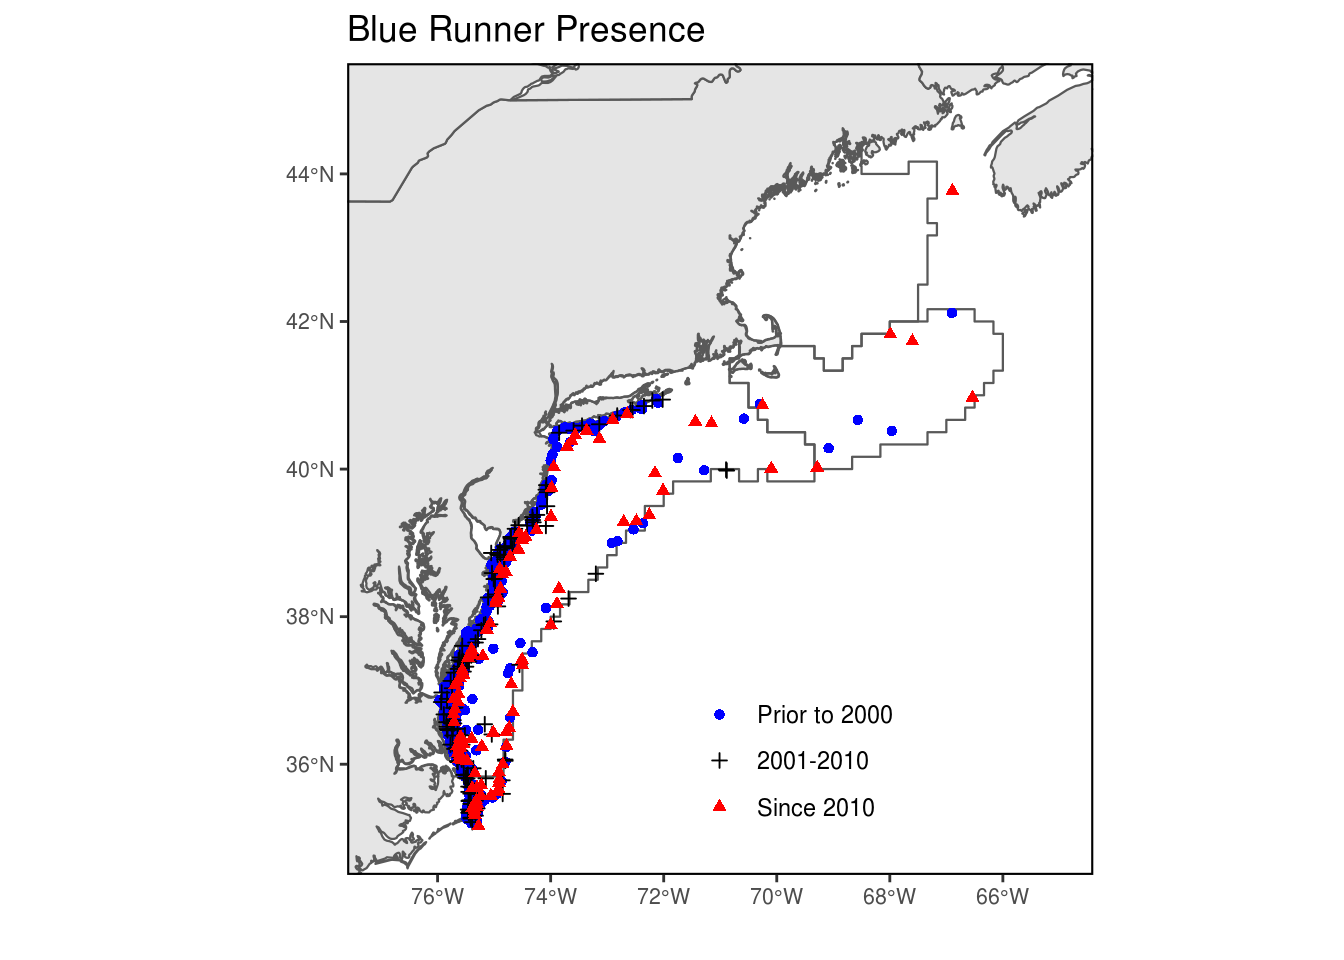
\includegraphics{/home/travis/build/NOAA-EDAB/tech-doc/images/unnamed-chunk-33-1.pdf}
\caption{\label{fig:unnamed-chunk-33}Blue runner presence on the Northeast shelf.}
\end{figure}

\hypertarget{ne-seabird-diet-and-productivity}{%
\chapter{NE Seabird diet and productivity}\label{ne-seabird-diet-and-productivity}}

\textbf{Description}: Common tern annual diet and productivity at seven Gulf of Maine colonies managed by the National Audubon Society's Seabird Restoration Program

\textbf{Indicator category}: Published method

\textbf{Found in}: State of the Ecosystem - New England (2019, 2020)

\textbf{Contributor(s)}: Don Lyons, Steve Kress, Paula Shannon, Sue Schubel

\textbf{Data steward}: Don Lyons, \href{mailto:dlyons@audubon.org}{\nolinkurl{dlyons@audubon.org}}

\textbf{Point of contact}: Don Lyons, \href{mailto:dlyons@audubon.org}{\nolinkurl{dlyons@audubon.org}}

\textbf{Public availability statement}: Please email \href{mailto:dlyons@audubon.org}{\nolinkurl{dlyons@audubon.org}} for further information and queries on this indicator source data.

\hypertarget{methods-33}{%
\section{Methods}\label{methods-33}}

\textbf{Chick diet}

Common tern (\emph{Sterna hirundo}) chick diet was quantified at each of the seven nesting sites (Fig. \ref{fig:nest-sites} ) by observing chick provisioning from portable observation blinds. The locations of observation blinds within each site were chosen to maximize the number of visible nests, and provisioning observations took place between mid-June and early August annually. Observations of chick diet were made during one or two, three to four hour periods throughout the day, but typically proceed according to nest activity levels (moreso in the morning hours). Observations began with chicks as soon as they hatched, and continue until the chicks fledged or died.

Most common tern prey species were identifiable to the species level due to distinct size, color and shape. However, when identification was not possible or was unclear, prey species were listed as ``unknown'' or ``unknown fish''. More detailed methods can be found in Hall, Kress, and Griffin (\protect\hyperlink{ref-hall2000}{2000}).

\textbf{Nest productivity}

Common tern nest productivity, in terms of the number of fledged chicks per nest, was collected annually from fenced enclosures at island nesting sites (known as ``productivity plots''). Newly hatched chicks within these enclosures were weighed, marked or banded, and observed until fledging, death, or until a 15 day period had passed when chicks were assumed to have fledged. Productivity was also quantified from observer blinds for nests outside of the productivity plots where chicks were marked for identification. More detailed methods for quantifying nest productivity can be found in Hall and Kress (\protect\hyperlink{ref-hall2004}{2004})

\hypertarget{data-sources-33}{%
\subsection{Data sources}\label{data-sources-33}}

Common tern diet and nest productivity data were provided by the National Audubon Society's Seabird Restoration Program.

\hypertarget{data-processing-23}{%
\subsection{Data processing}\label{data-processing-23}}

Diet and productivity data were formatted for inclusion in the \texttt{ecodata} R package using this R \href{https://github.com/NOAA-EDAB/ecodata/blob/master/data-raw/get_seabird_ne.R}{code}.

\hypertarget{data-analysis-31}{%
\subsection{Data analysis}\label{data-analysis-31}}

Raw diet data were used to create time series of mean shannon diversity through time and across study sites using the \texttt{vegan} R package (Oksanen et al. \protect\hyperlink{ref-R-vegan}{2019}). Code for this calculation can be found \href{https://github.com/NOAA-EDAB/tech-doc/blob/master/R/stored_scripts/seabird_ne_div_analysis.R}{here}. Diet diversity is presented along with nest productivity (+/- 1 SE).

Code used to create the figures below can be found at these links, \href{https://github.com/NOAA-EDAB/ecodata/blob/master/chunk-scripts/macrofauna.Rmd-tern-diet-diversity.R}{diet diversity}, \href{https://github.com/NOAA-EDAB/ecodata/blob/master/chunk-scripts/macrofauna.Rmd-stacked-bar-prey-freq.R}{prey frequencies} and \href{https://github.com/NOAA-EDAB/ecodata/blob/master/chunk-scripts/macrofauna.Rmd-aggregate-prod.R}{common tern productivity}

\hypertarget{plotting-25}{%
\subsection{Plotting}\label{plotting-25}}

\hypertarget{diet-diversity}{%
\subsubsection{Diet diversity}\label{diet-diversity}}

\begin{figure}

{\centering 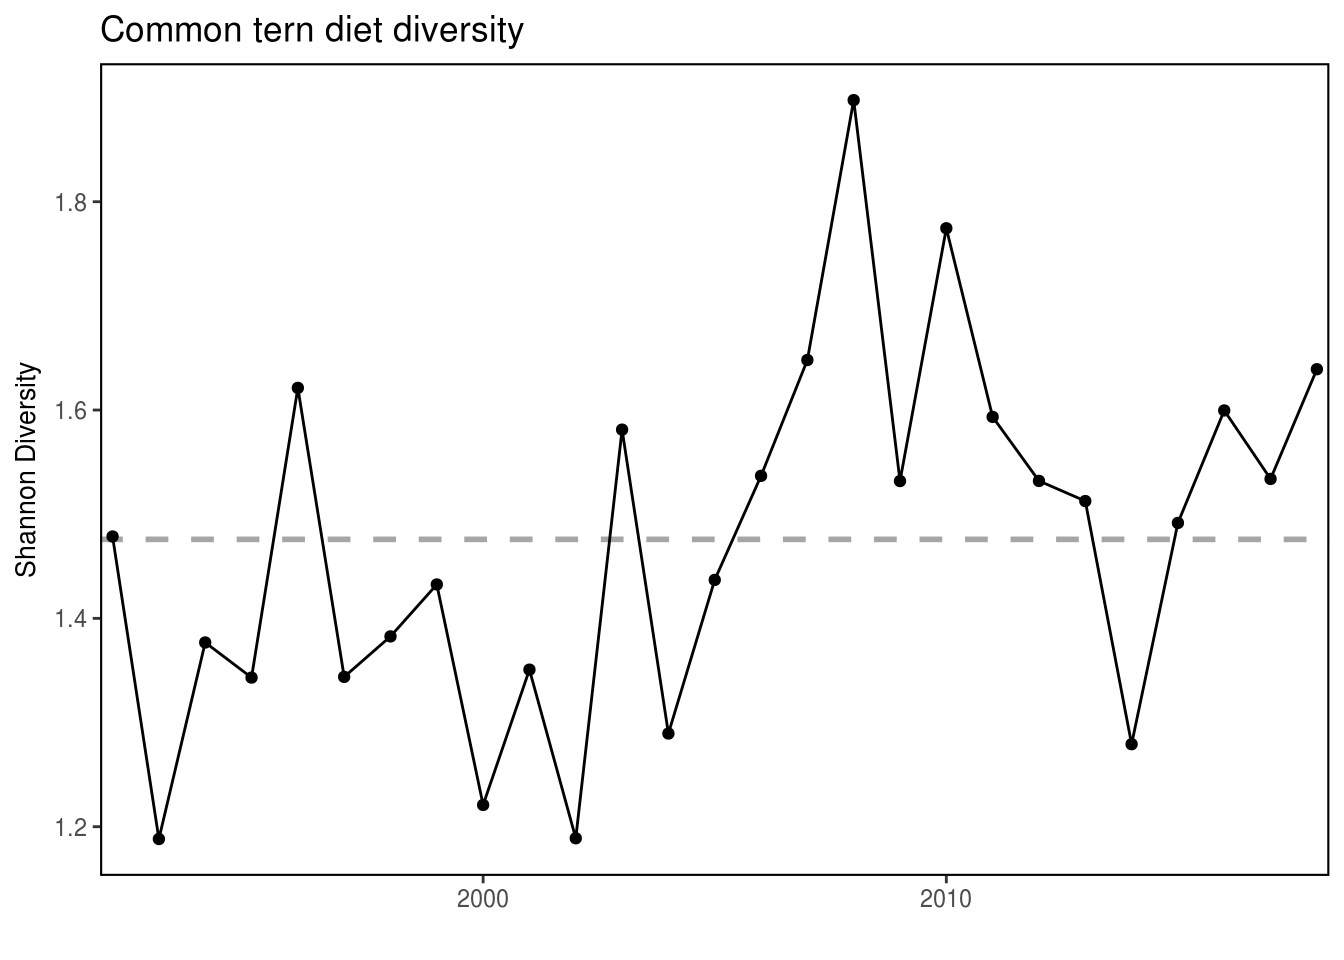
\includegraphics{/home/travis/build/NOAA-EDAB/tech-doc/images/unnamed-chunk-34-1} 

}

\caption{Shannon diversity of common tern diets observed at nesting sites in Gulf of Maine. Diversity of common tern diets has been predominantly above the long-term mean since 2006.}\label{fig:unnamed-chunk-34}
\end{figure}

\hypertarget{prey-frequencies}{%
\subsubsection{Prey frequencies}\label{prey-frequencies}}



\begin{figure}

{\centering 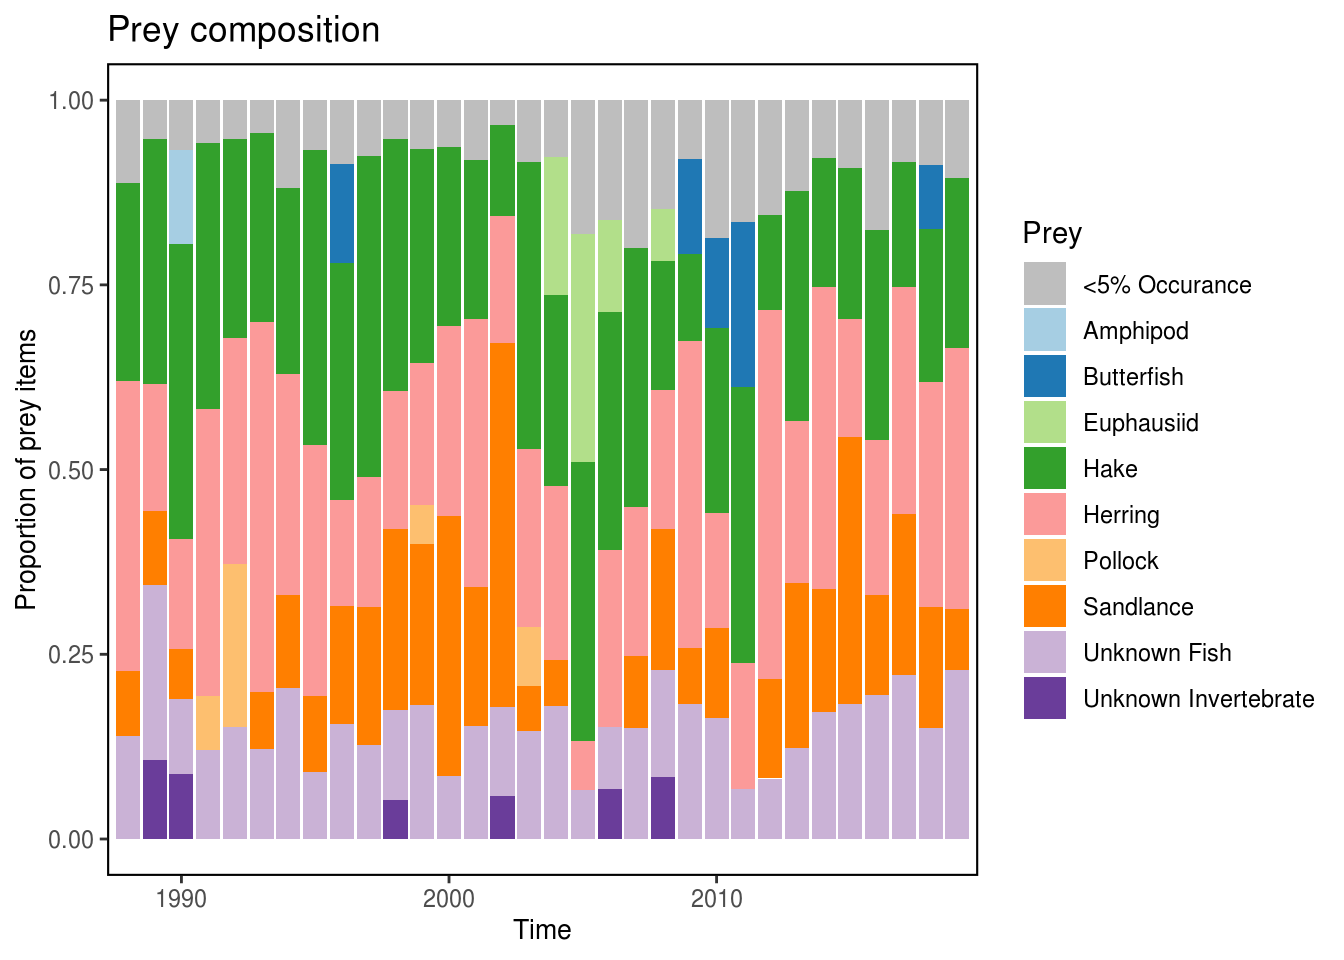
\includegraphics{/home/travis/build/NOAA-EDAB/tech-doc/images/unnamed-chunk-35-1} 

}

\caption{Prey frequencies in the diets of common tern observed across the seven colonies in the Gulf of Maine.}\label{fig:unnamed-chunk-35}
\end{figure}

\hypertarget{common-tern-productivity}{%
\subsubsection{Common tern productivity}\label{common-tern-productivity}}



\begin{figure}

{\centering \includegraphics{/home/travis/build/NOAA-EDAB/tech-doc/images/unnamed-chunk-36-1} 

}

\caption{Common terns: Mean common tern productivity at nesting sites in Gulf of Maine. Error bars show +/- 1 SE of the mean.}\label{fig:unnamed-chunk-36}
\end{figure}

\hypertarget{ma-waterbird-productivity}{%
\chapter{MA waterbird productivity}\label{ma-waterbird-productivity}}

\textbf{Description}: Virginia waterbird data

\textbf{Indicator category}: Published Results

\textbf{Found in}: State of the Ecosystem - Mid-Atantic (2020)

\textbf{Contributor(s)}: Ruth Boettcher

\textbf{Data steward}: Kimberly Bastille \href{mailto:kimberly.bastille@noaa.gov}{\nolinkurl{kimberly.bastille@noaa.gov}}

\textbf{Point of contact}: Kimberly Bastille \href{mailto:kimberly.bastille@noaa.gov}{\nolinkurl{kimberly.bastille@noaa.gov}}

\textbf{Public availability statement}: Data is publically available.

\hypertarget{methods-34}{%
\section{Methods}\label{methods-34}}

\hypertarget{data-sources-34}{%
\subsection{Data sources}\label{data-sources-34}}

Virginia colonial waterbird breeding pair population estimates derived from table 4 of ``Status and distribution of colonial waterbirds in coastal Virginia: 2018 breeding season.'' Center for Conservation Biology Technical Report Series, CCBTR-18-17. College of William and Mary \& Virginia Commonwealth University, Williamsburg, VA. Available at: \url{https://scholarworks.wm.edu/cgi/viewcontent.cgi?article=1237\&context=ccb_reports}

\hypertarget{data-analysis-32}{%
\subsection{Data analysis}\label{data-analysis-32}}

NA

\hypertarget{data-processing-24}{%
\subsection{Data processing}\label{data-processing-24}}

VA colonial waterbird data were formatted for inclusion in the \texttt{ecodata} R package using this \href{https://github.com/NOAA-EDAB/ecodata/blob/master/data-raw/get_seabird_MAB.R}{R code}.

\hypertarget{plotting-26}{%
\subsection{Plotting}\label{plotting-26}}

Code used to create the figure below can be found \href{https://github.com/NOAA-EDAB/ecodata/blob/master/chunk-scripts/macrofauna.Rmd-VA-cote.R}{here}.

\begin{figure}

{\centering \includegraphics{/home/travis/build/NOAA-EDAB/tech-doc/images/unnamed-chunk-37-1} 

}

\caption{Functional group population estimated derived from Table 4 of Watts, B. D., B. J. Paxton, R. Boettcher, and A. L. Wilke. 2019.}\label{fig:unnamed-chunk-37}
\end{figure}

\hypertarget{seasonal-sst-anomalies}{%
\chapter{Seasonal SST Anomalies}\label{seasonal-sst-anomalies}}

\textbf{Description}: Seasonal SST Anomalies

\textbf{Indicator category}: Database pull with analysis

\textbf{Found in}: State of the Ecosystem - Gulf of Maine \& Georges Bank (2018, 2019, 2020), State of the Ecosystem - Mid-Atlantic (2018, 2019, 2020)

\textbf{Contributor(s)}: Sean Hardison, Vincent Saba

\textbf{Data steward}: Kimberly Bastille, \href{mailto:kimberly.bastille@noaa.gov}{\nolinkurl{kimberly.bastille@noaa.gov}}

\textbf{Point of contact}: Kimberly Bastille, \href{mailto:kimberly.bastille@noaa.gov}{\nolinkurl{kimberly.bastille@noaa.gov}}

\textbf{Public availability statement}: Source data are available \href{https://www.esrl.noaa.gov/psd/data/gridded/data.noaa.oisst.v2.highres.html}{here}.

\hypertarget{methods-35}{%
\section{Methods}\label{methods-35}}

\hypertarget{data-sources-35}{%
\subsection{Data sources}\label{data-sources-35}}

Data for seasonal sea surface tempature anomalies (Fig. \ref{fig:MAB-SST}) were derived from the National Oceanographic and Atmospheric Administartion optimum interpolation sea surface temperature high resolution data set (\href{https://www.esrl.noaa.gov/psd/data/gridded/data.noaa.oisst.v2.highres.html}{NOAA OISST V2}) provided by NOAA Earth System Research Laboratory's Physical Science Division, Boulder, CO. The data extend from 1981 to present, and provide a 0.25° x 0.25° global grid of SST measurements (Reynolds et al. \protect\hyperlink{ref-Reynolds2007}{2007}).

\hypertarget{data-extraction-28}{%
\subsection{Data extraction}\label{data-extraction-28}}

Individual files containing daily mean SST data for each year during the period of 1981-present were downloaded from the \href{https://www.esrl.noaa.gov/psd/data/gridded/data.noaa.oisst.v2.highres.html}{OI SST V5 site}. Yearly data provided as layered rasters were masked according to the extent of Northeast US Continental Shelf. Data were split into three month seasons for (Winter = Jan, Feb, Mar; Spring = Apr, May, Jun; Summer = July, August, September; Fall = Oct, Nov, Dec).

\hypertarget{data-analysis-33}{%
\subsection{Data analysis}\label{data-analysis-33}}

We calculated the long-term mean (LTM) for each season-specific stack of rasters over the period of 1982-2010, and then subtracted the (LTM) from daily mean SST values to find the SST anomaly for a given year. The use of climatological reference periods is a standard procedure for the calculation of meteorological anomalies (WMO \protect\hyperlink{ref-WMO2017}{2017}). Prior to 2019 State of the Ecosystem reports, SST anomaly information made use of a 1982-2012 reference period. A 1982-2010 reference period was adopted to facilitate calculating anomalies from a standard \href{https://www.esrl.noaa.gov/psd/data/gridded/data.noaa.oisst.v2.highres.html}{NOAA ESRL} data set.

R code used in extraction and processing \href{https://github.com/NOAA-EDAB/ecodata/blob/master/data-raw/get_seasonal_oisst_anom_gridded.R}{gridded} and \href{https://github.com/NOAA-EDAB/ecodata/blob/master/data-raw/get_seasonal_oisst_anom.R}{timeseries} data can found in the \texttt{ecodata} package.

\hypertarget{plotting-27}{%
\subsection{Plotting}\label{plotting-27}}

Code used to build the figure below can be found \href{https://github.com/NOAA-EDAB/ecodata/blob/master/chunk-scripts/LTL.Rmd-MAB-SST-insitu.R}{here}.

\begin{figure}

{\centering \includegraphics{/home/travis/build/NOAA-EDAB/tech-doc/images/MAB-SST-1} 

}

\caption{MAB seasonal sea surface temperature time series overlaid onto 2019 seasonal spatial anomalies.}\label{fig:MAB-SST}
\end{figure}

\hypertarget{stockstatus}{%
\chapter{Single Species Status Indicator}\label{stockstatus}}

\textbf{Description}: Summary of the most recent stock assessment results for each assessed species.

\textbf{Found in}: State of the Ecosystem - Gulf of Maine \& Georges Bank (2017, 2018, 2019, 2020), State of the Ecosystem - Mid-Atlantic (2017, 2018, 2019, 2020)

\textbf{Indicator category}: Synthesis of published information

\textbf{Contributor(s)}: Sarah Gaichas, based on code and spreadsheets originally provided by Chris Legault

\textbf{Data steward}: Sarah Gaichas \href{mailto:sarah.gaichas@noaa.gov}{\nolinkurl{sarah.gaichas@noaa.gov}}

\textbf{Point of contact}: Sarah Gaichas \href{mailto:sarah.gaichas@noaa.gov}{\nolinkurl{sarah.gaichas@noaa.gov}}

\textbf{Public availability statement}: All stock assessment results are publicly available (see Data Sources). Summarized data are available \href{http://comet.nefsc.noaa.gov/erddap/tabledap/assess_soe_v1.htmlTable?No,Entity_Name,Science_Center,Assessment_Year,Last_Data_Year,Assessment_Level,Citation,Comments,Best_F,F_Year,Flimit,Fmsy,F_Flimit,F_Fmsy,Best_B,B_Year,B_Blimit,B_Bmsy,Stock_Level_Relative_to_Bmsy,Bmsy,Blim}{here}.

\hypertarget{methods-36}{%
\section{Methods}\label{methods-36}}

\hypertarget{data-sources-36}{%
\subsection{Data sources}\label{data-sources-36}}

``Data'' used for this indicator are the outputs of stock assessment models and review processes, including reference points (proxies for fishing mortality limits and stock biomass targets and limits), and the current fishing mortality rate and biomass of each stock. The spreadsheet summarizes the most recent stock assessment updates for each species, which are available on the Northeast Fisheries Science Center (NEFSC) website at:
\url{https://www.nefsc.noaa.gov/saw/reports.html}\\
\url{https://www.nefsc.noaa.gov/publications/crd/crd1717/}

Additional assessments are reported directly to the New England Fishery Management Council (NEFMC):
\url{http://s3.amazonaws.com/nefmc.org/Document-2-SAFE-Report-for-Fishing-Year-2016.pdf}\\
\url{http://s3.amazonaws.com/nefmc.org/4_NEFSC_SkateMemo_July_2017.pdf}

\hypertarget{data-extraction-29}{%
\subsection{Data extraction}\label{data-extraction-29}}

Each assessment document was searched to find the following information (often but not always summarized under a term of reference to determine stock status in the executive summary):

\begin{itemize}
\item
  \textbf{Bcur}: current year biomass, (most often spawning stock biomass (SSB) or whatever units the reference points are in)
\item
  \textbf{Fcur}: current year fishing mortality, F
\item
  \textbf{Bref}: biomass reference point, a proxy of Bmsy (the target)
\item
  \textbf{Fref}: fishing mortality reference point, a proxy of Fmsy
\end{itemize}

\hypertarget{data-processing-25}{%
\subsection{Data processing}\label{data-processing-25}}

R code used to process the stock status data set for inclusion in the \texttt{ecodata} R package can be found \href{https://github.com/NOAA-EDAB/ecodata/blob/master/data-raw/get_stocks.R}{here}.

\hypertarget{data-analysis-34}{%
\subsection{Data analysis}\label{data-analysis-34}}

For each assessed species, Bcur is divided by Bref and Fcur is divided by Fref. They are then plotted for each species on an x-y plot, with Bcur/Bref on the x axis, and Fcur/Fref on the y axis.

\hypertarget{plotting-28}{%
\subsection{Plotting}\label{plotting-28}}

The script used to develop the figure in the State of the Ecosystem report can be found \href{https://github.com/NOAA-EDAB/ecodata/blob/master/chunk-scripts/human_dimensions.Rmd-stock-status1.R}{here}.

\begin{figure}
\centering
\includegraphics{/home/travis/build/NOAA-EDAB/tech-doc/images/unnamed-chunk-39-1.pdf}
\caption{\label{fig:unnamed-chunk-39}Summary of single species status for MAFMC and jointly managed stocks.}
\end{figure}

\hypertarget{slopewater-proportions}{%
\chapter{Slopewater proportions}\label{slopewater-proportions}}

\textbf{Description}: Percent total of water type observed in the deep Northeast Channel (150-200 m water depth).

\textbf{Indicator category}: Published methods

\textbf{Found in}: State of the Ecosystem - Gulf of Maine \& Georges Bank (2019, 2020)

\textbf{Contributors}: Paula Fratantoni, \href{mailto:paula.fratantoni@noaa.gov}{\nolinkurl{paula.fratantoni@noaa.gov}}; David Mountain, NOAA Fisheries, retired.

\textbf{Data steward}: Kimberly Bastille, \href{mailto:kimberly.bastille@noaa.gov}{\nolinkurl{kimberly.bastille@noaa.gov}}

\textbf{Point of contact}: Paula Fratantoni, \href{mailto:paula.fratantoni@noaa.gov}{\nolinkurl{paula.fratantoni@noaa.gov}}

\textbf{Public availability statement}: Source data are publicly available at \url{ftp://ftp.nefsc.noaa.gov/pub/hydro/matlab_files/yearly} and in the World Ocean Database housed at \url{http://www.nodc.noaa.gov/OC5/SELECT/dbsearch/dbsearch.html} under institute code 258

\hypertarget{methods-37}{%
\section{Methods}\label{methods-37}}

\hypertarget{data-sources-37}{%
\subsection{Data sources}\label{data-sources-37}}

The slope water composition index incorporates temperature and salinity measurements collected on Northeast Fisheries Science Center surveys between 1977-present within the geographic confines of the Northeast Channel in the Gulf of Maine. Early measurements were made using water samples collected primarily with Niskin bottles at discreet depths, mechanical bathythermographs and expendable bathythermograph probes, but by 1991 the CTD -- an acronym for conductivity temperature and depth -- became standard equipment on all NEFSC surveys.

\hypertarget{data-extraction-30}{%
\subsection{Data extraction}\label{data-extraction-30}}

While all processed hydrographic data are archived in an Oracle database (OCDBS), we work from Matlab-formatted files stored locally.

\hypertarget{data-analysis-35}{%
\subsection{Data analysis}\label{data-analysis-35}}

Temperature and salinity measurements are examined to assess the composition of the waters entering the Gulf of Maine through the Northeast Channel. The analysis closely follows the methodology described by D. G. Mountain (\protect\hyperlink{ref-mountain2012}{2012}). This method assumes that the waters flowing into the Northeast Channel between 150 and 200 meters depth are composed of slope waters, originating offshore of the continental shelf, and shelf waters, originating on the continental shelf south of Nova Scotia.

For each survey in the hydrographic archive, ocean temperature and salinity observations sampled in the area just inside the Northeast Channel (bounded by 42.2-42.6\textdegree latitude north and 66-66.8\textdegree longitude west) and between 150 - 200 meters depth are extracted and a volume-weighted average temperature and salinity is calculated. The volume weighting is accomplished by apportioning the area within the Northeast Channel polygon among the stations occupying the region, based on inverse distance squared weighting. The result of this calculation is a timeseries of volume-average temperature and salinity having a temporal resolution that matches the survey frequency in the database.

The average temperature and salinity observed at depth in the Northeast Channel is assumed to be the product of mixing between three distinct sources having the following temperature and salinity characteristics: (1) Warm Slope Water (T=10 \textdegree C, S=35), (2) Labrador Slope Water (T=6 \textdegree C, S=34.7) and (3) Scotian Shelf Water (T=2 \textdegree C, S=32). As described by D. G. Mountain (\protect\hyperlink{ref-mountain2012}{2012}), the relative proportion of each source is determined via a rudimentary 3-point mixing algorithm. On a temperature-salinity diagram, lines connecting the T-S coordinates for these three sources form a triangle, the sides of which represent mixing lines between the sources. A water sample that is a mixture of two sources will have a temperature and salinity that falls somewhere along the line connecting the two sources on the temperature-salinity diagram. Observations of temperature and salinity collected within the Northeast Channel would be expected to fall within the triangle if the water sampled is a mixture of the three sources. Simple geometry allows us to calculate the relative proportion of each source in a given measurement. As an example, a line drawn from the T-S point representing shelf water through an observed T-S in the center of the triangle will intersect the opposite side of the triangle (the mixing line connecting the coordinates of the two slope water sources). This intersecting T-S value may then be used to calculate the relative proportions (percentage) of the two slope water sources. Using this method, the percentage of Labrador slope water and Warm slope water are determined for the timeseries of volume-average temperature and salinity.

It should be noted that our method assumes that the temperature and salinity properties associated with the source watermasses are constant. In reality, these may vary from year to year, modified by atmospheric forcing, mixing and/or advective processes. Likewise, other sources are periodically introduced into the Northeast Channel, including intrusions of Gulf Stream water flowing into the Gulf of Maine and modified shelf water flowing out of the Gulf of Maine along the flank of Georges Bank. These sources are not explicitely considered in the 3-point mixing algorithm and may introduce errors in the proportional estimates. Code used to calculate slopewater proportions can be found \href{https://github.com/NOAA-EDAB/tech-doc/blob/master/R/stored_scripts/slopewater_analysis.R}{here}.

\hypertarget{data-processing-26}{%
\subsection{Data processing}\label{data-processing-26}}

Source data were formatted for inclusion in the \texttt{ecodata} R package using the R code found \href{https://github.com/NOAA-EDAB/ecodata/blob/master/data-raw/get_slopewater.R}{here}.

\hypertarget{plotting-29}{%
\subsection{Plotting}\label{plotting-29}}

Code used to create the figure below can be found \href{https://github.com/NOAA-EDAB/ecodata/blob/master/chunk-scripts/LTL.Rmd-wsw-prop.R}{here}.

\begin{figure}

{\centering \includegraphics{/home/travis/build/NOAA-EDAB/tech-doc/images/unnamed-chunk-40-1} 

}

\caption{Proportion of warm slope water (WSW) and Labrador slope water (LSLW) entering the GOM through the Northeast Channel.}\label{fig:unnamed-chunk-40}
\end{figure}

\hypertarget{species-density-estimates}{%
\chapter{Species Density Estimates}\label{species-density-estimates}}

\textbf{Description}: Current and Historical Species Distributions

\textbf{Found in}: State of the Ecosystem - Gulf of Maine \& Georges Bank (2017, 2018), State of the Ecosystem - Mid-Atlantic (2017, 2018)

\textbf{Indicator category}: Database pull; Database pull with analysis

\textbf{Contributor}: Kevin Friedland

\textbf{Data steward}: Kevin Friedland

\textbf{Point of contact}: Kevin Friedland, \href{mailto:kevin.friedland@noaa.gov}{\nolinkurl{kevin.friedland@noaa.gov}}

\textbf{Public availability statement}: Source data are publicly available.

\hypertarget{methods-38}{%
\section{Methods}\label{methods-38}}

We used kernel density plots to depict shifts in species' distributions over time. These figures characterize the probability of a species occurring in a given area based on Northeast Fisheries Science Center (NEFSC) Bottom Trawl Survey data. Kernel density estimates (KDEs) of distributions are shown for the period of 1970-1979 (shaded blue) and most recent three years of survey data (shaded red) (e.g.~Figure \ref{fig:kde-fig}). Results are typically visualized for spring and fall bottom trawl surveys seperately.

Three probability levels (25\%, 50\%, 75\%) are shown for each time period, where the 25\% region depicts the core area of the distribution and the 75\% region shows the area occupied more broadly by the species. A wide array of KDEs for many ecologically and economically important species on the Northeast US Continental Shelf are available \href{https://www.nefsc.noaa.gov/ecosys/current-conditions/kernel-density.html}{here}.

\hypertarget{data-sources-38}{%
\subsection{Data sources}\label{data-sources-38}}

Current and historical species distributions are based on the NEFSC Bottom Trawl Survey data (aka \protect\hyperlink{survdat}{``Survdat''}) and depth strata. Strata are available as shapefiles that can be downloaded \href{https://github.com/NOAA-EDAB/tech-doc/tree/master/gis}{here} (listed as
``strata.shp'').

\hypertarget{data-analysis-36}{%
\subsection{Data analysis}\label{data-analysis-36}}

Code used for species density analysis can be found \href{https://github.com/NOAA-EDAB/tech-doc/blob/master/R/stored_scripts/species_density_analysis.R}{here}.

\hypertarget{plotting-30}{%
\subsection{Plotting}\label{plotting-30}}

\begin{figure}
\centering
\includegraphics{/home/travis/build/NOAA-EDAB/tech-doc/images/kde-fig-1.pdf}
\caption{\label{fig:kde-fig}Current and historical sea scallop kernel density estimates derived from spring survey data. Current estimates derived from 2016-2018 data.}
\end{figure}

\hypertarget{species-distribution-indicators}{%
\chapter{Species Distribution Indicators}\label{species-distribution-indicators}}

\textbf{Description}: Species mean depth, along-shelf distance, and distance to coastline

\textbf{Found in}: State of the Ecosystem - Gulf of Maine \& Georges Bank (2017, 2018, 2019, 2020), State of the Ecosystem - Mid-Atlantic (2017, 2018, 2019, 2020)

\textbf{Indicator category}: Extensive analysis; not yet published

\textbf{Contributor(s)}: Kevin Friedland

\textbf{Data steward}: Kevin Friedland, \href{mailto:kevin.friedland@noaa.gov}{\nolinkurl{kevin.friedland@noaa.gov}}

\textbf{Point of contact}: Kevin Friedland, \href{mailto:kevin.friedland@noaa.gov}{\nolinkurl{kevin.friedland@noaa.gov}}

\textbf{Public availability statement}: Source data are available upon request (read more \href{https://inport.nmfs.noaa.gov/inport/item/22560}{here}). Derived data may be downloaded \href{https://comet.nefsc.noaa.gov/erddap/tabledap/SOE_habitat_soe_v1.html}{here}.

\hypertarget{methods-39}{%
\section{Methods}\label{methods-39}}

Three metrics quantifying spatial-temporal distribution shifts within fish populations were developed by Friedland et al. (\protect\hyperlink{ref-Friedland2018}{2018}), including mean depth, along-shelf distance, and distance to coastline. Along-shelf distance is a metric for quantifying the distribution of a species through time along the axis of the US Northeast Continental Shelf, which extends northeastward from the Outer Banks of North Carolina. Values in the derived time series correspond to mean distance in km from the southwest origin of the along-shelf axis at 0 km. The along-shelf axis begins at 76.53°W 34.60°N and terminates at 65.71°W 43.49°N.

Once mean distance is found, depth of occurrence and distance to coastline can be calculated for each species' positional center. Analyses present in the State of the Ecosystem (SOE) reports include mean depth and along-shelf distance for Atlantic cod, sea scallop, summer flounder, and black sea bass.

\hypertarget{data-sources-39}{%
\subsection{Data sources}\label{data-sources-39}}

Data for these indicators were derived from fishery-independent bottom trawl survey data collected by the Northeast Fisheries Science Center (NEFSC).

\hypertarget{data-analysis-37}{%
\subsection{Data analysis}\label{data-analysis-37}}

Species distribution indicators were derived using the R code found \href{https://github.com/NOAA-EDAB/tech-doc/blob/master/R/stored_scripts/species_distribution_analysis.R}{here}.

\hypertarget{data-processing-27}{%
\subsection{Data processing}\label{data-processing-27}}

Distribution indicators were further formatted for inclusion in the \texttt{ecodata} R package using the R code found \href{https://github.com/NOAA-EDAB/ecodata/blob/master/data-raw/get_species_dist.R}{here}.

\hypertarget{plotting-31}{%
\subsection{Plotting}\label{plotting-31}}

Code used to create the figure below can be found \href{https://github.com/NOAA-EDAB/ecodata/blob/master/chunk-scripts/macrofauna.Rmd-spec-dist.R}{here}.
\includegraphics{/home/travis/build/NOAA-EDAB/tech-doc/images/unnamed-chunk-42-1.pdf}

\hypertarget{stomach-fullness}{%
\chapter{Stomach fullness}\label{stomach-fullness}}

\textbf{Description}: Stomach Fullness

\textbf{Found in}: State of the Ecosystem - Mid-Atlantic (2020), State of the Ecosystem - New England (2020)

\textbf{Indicator category}: Database pull with analysis

\textbf{Contributor(s)}: Laurel Smith

\textbf{Data steward}: Kimberly Bastille \href{mailto:kimberly.bastille@noaa.gov}{\nolinkurl{kimberly.bastille@noaa.gov}}

\textbf{Point of contact}: Kimberly Bastille \href{mailto:kimberly.bastille@noaa.gov}{\nolinkurl{kimberly.bastille@noaa.gov}}

\textbf{Public availability statement}: NEFSC survey data used in these analyses are available upon request (see \href{https://inport.nmfs.noaa.gov/inport}{Food Habits Database (FHDBS)} for access procedures). Derived stomach fullness data are available \href{https://comet.nefsc.noaa.gov/erddap/tabledap/}{here} (STILL NEEDS SOE DATA REFERENCE!).

\hypertarget{methods-40}{%
\section{Methods}\label{methods-40}}

An index of stomach fullness was calculated from NEFSC autumn bottom trawl food habits data, as a simple ratio of estimated stomach content weight to total weight of an individual fish. Stomach fullness may be a better measure than absolute stomach weight if combining across species into a feeding guild, to prevent larger animals with heavier stomachs from dominating the index. An average stomach fullness was calcuated annually for each species and Ecological Production Unit (EPU).

\hypertarget{data-sources-40}{%
\subsection{Data sources}\label{data-sources-40}}

Stomach contents weights and individual fish weights (both to the nearest gram) were collected on the NEFSC bottom trawl surveys from 1992-present aboard RVs Albatross IV, Delaware II and the Henry B. Bigelow (see \href{https://inport.nmfs.noaa.gov/inport}{Food Habits Database (FHDBS)} for access procedures).

\hypertarget{data-extraction-31}{%
\subsection{Data extraction}\label{data-extraction-31}}

NEFSC food habits data summarized in the R data file allfh.RData were obtained from Brian Smith (\href{mailto:Brian.Smith@noaa.gov}{\nolinkurl{Brian.Smith@noaa.gov}}) for this index.

\hypertarget{data-analysis-38}{%
\subsection{Data analysis}\label{data-analysis-38}}

The stomach fullness index was calculated using the R script found \href{https://github.com/Laurels1/StomachFullness}{here}.

\hypertarget{data-processing-28}{%
\subsection{Data processing}\label{data-processing-28}}

Fish stomach fullness index was formatted for inclusion in the \texttt{ecodata} R package using this \href{https://github.com/NOAA-EDAB/ecodata/blob/master/data-raw/get_stom_fullness.R}{R code}. Stomach fullness was expressed as an annual anomaly for each species in each region.

\hypertarget{plotting-32}{%
\subsection{Plotting}\label{plotting-32}}

The plot below was built using the code found
\href{https://github.com/NOAA-EDAB/ecodata/blob/master/chunk-scripts/macrofauna.Rmd-ma-stomachs.R}{here}.

\begin{figure}
\centering
\includegraphics{/home/travis/build/NOAA-EDAB/tech-doc/images/unnamed-chunk-43-1.pdf}
\caption{\label{fig:unnamed-chunk-43}Stomach fullness anomaly.}
\end{figure}

\hypertarget{survdat}{%
\chapter{Survey Data}\label{survdat}}

\textbf{Description}: Survdat (Survey database)

\textbf{Found in}: State of the Ecosystem - Gulf of Maine \& Georges Bank (2017, 2018, 2019, 2020), State of the Ecosystem - Mid-Atlantic (2017, 2018, 2019, 2020)

\textbf{Indicator category}: Database pull

\textbf{Contributor(s)}: Sean Lucey

\textbf{Data steward}: Sean Lucey \href{mailto:sean.lucey@noaa.gov}{\nolinkurl{sean.lucey@noaa.gov}}

\textbf{Point of contact}: Sean Lucey \href{mailto:sean.lucey@noaa.gov}{\nolinkurl{sean.lucey@noaa.gov}}

\textbf{Public availability statement}: Source data are available to qualified researchers upon request (see ``Access Information'' \href{https://inport.nmfs.noaa.gov/inport/item/22560}{here}). Derived data used in SOE reports are available \href{https://comet.nefsc.noaa.gov/erddap/tabledap/group_landings_soe_v1.html}{here}.

\hypertarget{methods-41}{%
\section{Methods}\label{methods-41}}

The Northeast Fisheries Science Center (NEFSC) has been conducting standardized bottom trawl surveys
in the fall since 1963 and spring since 1968. The surveys follow a stratified random design. Fish
species and several invertebrate species are enumerated on a tow by tow basis (Azarovitz \protect\hyperlink{ref-Azarovitz1981}{1981}).\\
The data are housed in the NEFSC's survey database (SVDBS) maintained by the Ecosystem Survey Branch.

Direct pulls from the database are not advisable as there have been several gear modifications and
vessel changes over the course of the time series (Miller et al. \protect\hyperlink{ref-Miller_2010}{2010}). Survdat was developed as a database
query that applies the appropriate calibration factors for a seamless time series since the 1960s.
As such, it is the base for many of the other analyses conducted for the State of the Ecosystem
report that involve fisheries independent data.

The Survdat script can be broken down into two sections. The first pulls the raw data from SVDBS.
While the script is able to pull data from more than just the spring and fall bottom trawl surveys,
for the purposes of the State of the Ecosystem reports only the spring and fall data are used.
Survdat identifies those research cruises associated with the seasonal bottom trawl surveys and pulls
the station and biological data. Station data includes tow identification (cruise, station,
and stratum), tow location and date, as well as several environmental variables (depth, surface/bottom salinity,
and surface/bottom temperature). Stations are filtered for representativness using a station, haul, gear
(SHG) code for tows prior to 2009 and a tow, operations, gear, and aquisition (TOGA) code from 2009
onward. The codes that correspond to a representative tow (SHG \textless= 136 or TOGA \textless= 1324) are the same
used by assessment biologists at the NEFSC. Biological data includes the total biomass and abundance
by species, as well as lengths and number at length.

The second section of the Survdat script applies the calibration factors. There are four calibrartion
factors applied (Table \ref{tab:calibration}). Calibration factors are pulled directly from SVDBS. Vessel conversions were made from
either the NOAA Ship \emph{Delaware II} or NOAA Ship \emph{Henry Bigelow} to the NOAA Ship \emph{Albatross IV} which was
the primary vessel for most of the time series. The Albatross was decommisioned in 2009 and the Bigelow is
now the primary vessel for the bottom trawl survey.

\begin{table}

\caption{\label{tab:calibration}Calibration factors for NEFSC trawl survey data}
\centering
\begin{tabular}[t]{lll}
\toprule
Name & Code & Applied\\
\midrule
Door Conversion & DCF & <1985\\
Net Conversion & GCF & 1973 - 1981 (Spring)\\
Vessel Conversion I & VCF & Delaware II records\\
Vessel Conversion II & BCF & Henry Bigelow records\\
\bottomrule
\end{tabular}
\end{table}

The output from Survdat is an RData file that contains all the station and biological data, corrected
as noted above, from the NEFSC Spring Bottom Trawl Survey and NEFSC Fall Bottom Trawl Survey. The RData
file is a data.table, a powerful wrapper for the base data.frame (\url{https://cran.r-project.org/web/packages/data.table/data.table.pdf}).
There are also a series of tools that have been developed in order to utilize the Survdat data set
(\url{https://github.com/slucey/RSurvey}).

\hypertarget{data-sources-41}{%
\subsection{Data sources}\label{data-sources-41}}

Survdat is a database query of the NEFSC survey database (SVDBS).These data are available to qualified researchers upon request. More information on the data request process is available under the ``Access Information'' field \href{https://inport.nmfs.noaa.gov/inport/item/22560}{here}.

\hypertarget{data-extraction-32}{%
\subsection{Data extraction}\label{data-extraction-32}}

Extraction methods are described above. The R code found \href{https://github.com/slucey/RSurvey/blob/master/Survdat.r}{here} was used in the survey data extraction process.

\hypertarget{data-analysis-39}{%
\subsection{Data analysis}\label{data-analysis-39}}

The fisheries independent data contained within the Survdat is used in a variety of
products; the more complicated analyses are detailed in their own sections. The most straightforward use of this data is for the resource species aggregate biomass
indicators. For the purposes of the aggregate biomass indicators, fall and spring
survey data are treated separately. Additionally, all length data is dropped and
species seperated by sex at the catch level are merged back together.

Since 2020, survey strata where characterized as being within an \protect\hyperlink{epu}{Ecological Production Unit}
based on where at least 50\% of the area of the strata was located (Figure \ref{fig:epustrata}. While this does not
create a perfect match for the EPU boundaries it allows us to calculate the variance
associated with the index as the survey was designed.

\textbackslash begin\{figure\}

\{\centering \includegraphics[width=26.39in]{/home/travis/build/NOAA-EDAB/tech-doc/images/EPU_Designations_Map}

\}

\textbackslash caption\{Map of the Northeast Shelf broken into the four Ecological Production Units by strata. Strata were assigned to an EPU based on which one contained at least 50\% of the area of the strata.\}\label{fig:epustrata}
\textbackslash end\{figure\}

Prior to 2020, Survdat was first post stratified into EPUs by labeling stations by the EPU they fell within
using the \texttt{over} function from the \texttt{rgdal} R package (Bivand, Keitt, and Rowlingson \protect\hyperlink{ref-rgdal}{2018}). Next, the total number
of stations within each EPU per year is counted using unique station records. Biomass
is summed by species per year per EPU. Those sums are divided by the appropriate
station count to get the EPU mean. Finally, the mean biomasses are summed by \protect\hyperlink{aggroups}{aggregate groups}. These steps are encompassed in the \href{https://github.com/NOAA-EDAB/ecodata/blob/master/data-raw/get_agg_bio.R}{processing code}, which also includes steps taken to format the data set for inclusion in the \texttt{ecodata} R package.

\hypertarget{plotting-33}{%
\subsection{Plotting}\label{plotting-33}}

Code used to create the figure below can be found \href{https://github.com/NOAA-EDAB/ecodata/blob/master/chunk-scripts/macrofauna.Rmd-agg-bio.R}{here}

\begin{figure}
\centering
\includegraphics{/home/travis/build/NOAA-EDAB/tech-doc/images/unnamed-chunk-44-1.pdf}
\caption{\label{fig:unnamed-chunk-44}Spring (left) and fall (right) surveyed biomass in the Mid-Atlantic Bight. Data from the NEFSC Bottom Trawl Survey are shown in black, with NEAMAP shown in red.}
\end{figure}

\hypertarget{thermal-habitat-projections}{%
\chapter{Thermal Habitat Projections}\label{thermal-habitat-projections}}

\textbf{Description}: Species Thermal Habitat Projections

\textbf{Found in}: State of the Ecosystem - Gulf of Maine \& Georges Bank (2018), State of the Ecosystem - Mid-Atlantic (2018)

\textbf{Indicator category}: Published methods

\textbf{Contributor(s)}: Vincent Saba

\textbf{Data steward}: Vincent Saba, \href{mailto:vincent.saba@noaa.gov}{\nolinkurl{vincent.saba@noaa.gov}}

\textbf{Point of contact}: Vincent Saba, \href{mailto:vincent.saba@noaa.gov}{\nolinkurl{vincent.saba@noaa.gov}}

\textbf{Public availability statement}: Source data are available to the public. Model outputs for thermal habitat projections are available \href{https://comet.nefsc.noaa.gov/erddap/info/index.html?page=1\&itemsPerPage=1000}{here}.

\hypertarget{methods-42}{%
\section{Methods}\label{methods-42}}

This indicator is based on work reported in Kleisner et al. (\protect\hyperlink{ref-Kleisner2017}{2017}).

\hypertarget{data-sources-42}{%
\subsection{Data sources}\label{data-sources-42}}

\hypertarget{global-climate-model-projection}{%
\subsubsection{Global Climate Model Projection}\label{global-climate-model-projection}}

We used \href{https://www.gfdl.noaa.gov/high-resolution-climate-modeling/}{National Oceanographic and Atmosheric Administration's Geophysical Fluid Dynamics Laboratory (NOAA GFDL) CM2.6 simulation} consisting of (1) a 1860 pre-industrial control, which brings the climate system into near-equilibrium with 1860 greenhouse gas concentrations, and (2) a transient climate response (2xCO2) simulation where atmospheric CO2 is increased by 1\% per year, which results in a doubling of CO2 after 70 years. The climate change response from CM2.6 was based on the difference between these two experimental runs. Refer to Saba et al. (\protect\hyperlink{ref-Saba2016}{2016}) for further details.

\hypertarget{modeling-changes-in-suitable-thermal-habitat}{%
\subsubsection{Modeling Changes in Suitable Thermal Habitat}\label{modeling-changes-in-suitable-thermal-habitat}}

The NOAA Northeast Fisheries Science Center, U.S. Northeast Shelf (NES) bottom trawl survey, which has been conducted for almost 50-years in the spring and fall, provides a rich source of data on historical and current marine species distribution, abundance, and habitat, as well as oceanographic conditions (Azarovitz \protect\hyperlink{ref-Azarovitz1981}{1981}). The survey was implemented to meet several objectives: (1) monitor trends in abundance, biomass, and recruitment, (2) monitor the geographic distribution of species, (3) monitor ecosystem changes, (4) monitor changes in life history traits (e.g., trends in growth, longevity, mortality, and maturation, and food habits), and (5) collect baseline oceanographic and environmental data. These data can be leveraged for exploring future changes in the patterns of abundance and distribution of species in the region.

\hypertarget{data-analysis-40}{%
\subsection{Data analysis}\label{data-analysis-40}}

\hypertarget{global-climate-model-projection-1}{%
\subsubsection{Global Climate Model Projection}\label{global-climate-model-projection-1}}

The CM2.6 80-year projections can be roughly assigned to a time period by using the International Panel on Climate Change (IPCC) Representative Concentration Pathways (RCPs), which describe four different 21st century pathways of anthropogenic greenhouse gas emissions, air pollutant emissions, and land use (IPCC \protect\hyperlink{ref-IPCC2014}{2014}). There are four RCPs, ranging from a stringent mitigation scenario (RCP2.6), two intermediate scenarios (RCP4.5 and RCP6.0), and one scenario with very high greenhouse gas emissions (RCP8.5). For RCP8.5, the global average temperature at the surface warms by 2C by approximately 2060-2070 relative to the 1986-2005 climatology (see Figure SPM.7a in \href{https://www.ipcc.ch/pdf/assessment-report/ar5/wg1/WG1AR5_SPM_FINAL.pdf}{IPCC, 2013}). For CM2.6, the global average temperature warms by 2C by approximately years 60-80 (see Fig. 1 in Winton et al. (\protect\hyperlink{ref-winton_has_2014}{2014})). Therefore, the last 20 years of the transient climate response simulation roughly corresponds to 2060-2080 of the RCP8.5 scenario.

Here, the monthly differences in surface and bottom temperatures (`deltas') for spring (February-April) and fall (September- November) are added to an average annual temperature climatology for spring and fall, respectively, derived from observed surface and bottom temperatures to produce an 80-year time series of future bottom and surface temperatures in both seasons. The observed temperatures come from the NEFSC spring and fall bottom trawl surveys conducted from 1968 to 2013 and represent approximately 30,000 observations over the time series.

\hypertarget{modeling-changes-in-suitable-thermal-habitat-1}{%
\subsubsection{Modeling Changes in Suitable Thermal Habitat}\label{modeling-changes-in-suitable-thermal-habitat-1}}

We modeled individual species thermal habitat across the whole U.S. NES and not by sub-region because we did not want to assume that species would necessarily maintain these assemblages in the future. Indeed, the goal here is to determine future patterns of thermal habitat availability for species on the U.S. NES in more broad terms. We fit one generalizaed additive model (GAM) based on both spring and fall data (i.e., an annual model as opposed to separate spring and fall models) and use it to project potential changes in distribution and magnitude of biomass separately for each season for each species. By creating a single annual model based on temperature data from both spring and fall, we ensure that the full thermal envelope of each species is represented. For example, if a species with a wide thermal tolerance has historically been found in cooler waters in the spring, and in warmer waters in the fall, an annual model will ensure that if there are warmer waters in the spring in the future, that species will have the potential to inhabit those areas. Additionally, because the trawl survey data are subject to many zero observations, we use delta-lognormal GAMs (Wood \protect\hyperlink{ref-Wood2011a}{2011}), which model presence-absence separately from logged positive observations. The response variables in each of the GAMs are presence/absence and logged positive biomass of each assemblage or individual species, respectively. A binomial link function is used in the presence/absence models and a Gaussian link function is used in the models with logged positive biomass.
The predictor variables are surface and bottom temperature and depth (all measured by the survey at each station), fit with penalized regression splines, and survey stratum, which accounts for differences in regional habitat quality across the survey region. Stratum may be considered to account for additional information not explicitly measured by the survey (e.g., bottom rugosity). Predictions of species abundance are calculated as the product of the predictions from the presence-absence model, the exponentiated predictions from the logged positive biomass model, and a correction factor to account for the retransformation bias associated with the log transformation (Duan \protect\hyperlink{ref-Duan1983}{1983}; and see Pinsky et al. \protect\hyperlink{ref-Pinsky2013}{2013}).

We calculated the suitable thermal habitat both in terms of changes in `suitable thermal abundance', defined as the species density possible given appropriate temperature, depth and bathymetric conditions, and changes in `suitable thermal area', defined as the size of the physical area potentially occupied by a species given appropriate temperature, depth and bathymetric conditions. Suitable thermal abundance is determined from the predictions from the GAMs (i.e., a prediction of biomass). However, this quantity should not be interpreted directly as a change in future abundance or biomass, but instead as the potential abundance of a species in the future given changes in temperature and holding all else (e.g., fishing effort, species interactions, productivity, etc.) constant. Suitable thermal area is determined as a change in the suitable area that a species distribution occupies in the future and is derived from the area of the kernel density of the distribution. To ensure that the estimates are conservative, we select all points with values greater than one standard deviation above the mean. We then compute the area of these kernels using the \texttt{gArea} function from the \texttt{rgeos} package in R (Bivand et al. \protect\hyperlink{ref-Bivand2011}{2011}).

\hypertarget{plotting-34}{%
\subsection{Plotting}\label{plotting-34}}

\begin{figure}
\centering
\includegraphics{/home/travis/build/NOAA-EDAB/tech-doc/images/th-maps-1.pdf}
\caption{\label{fig:th-maps}Current thermal habitat estimate (A), and 20-40 year thermal habitat projection (B) for summer flounder on the Northeast Continental Shelf.}
\end{figure}

\textbf{Note}: The thermal habitat model output for all species presented in State of the Ecosystem reports is accessible through the \href{https://comet.nefsc.noaa.gov/erddap/info/index.html?page=1\&itemsPerPage=1000}{NEFSC ERDDAP server}.

\hypertarget{trend-analysis}{%
\chapter{Trend Analysis}\label{trend-analysis}}

\textbf{Description}: Time series trend analysis

\textbf{Found in}: State of the Ecosystem - Gulf of Maine \& Georges Bank (2018, 2019), State of the Ecosystem - Mid-Atlantic (2018, 2019)

\textbf{Indicator category}: Extensive analysis, not yet published

\textbf{Contributor(s)}: Sean Hardison, Charles Perretti, Geret DePiper

\textbf{Data steward}: NA

\textbf{Point of contact}: Kimberly Bastille, \href{mailto:kimberly.bastille@noaa.gov}{\nolinkurl{kimberly.bastille@noaa.gov}}

\textbf{Public availability statement}: NA

\hypertarget{methods-43}{%
\section{Methods}\label{methods-43}}

Summarizing trends for ecosystem indicators is desirable, but the power of statistical tests to detect a trend is hampered by low sample size and autocorrelated observations (see Nicholson and Jennings \protect\hyperlink{ref-Nicholson2004}{2004}; Wagner et al. \protect\hyperlink{ref-Wagner2013}{2013}; Storch \protect\hyperlink{ref-VonStorch1999a}{1999}). Prior to 2018, time series indicators in State of the Ecosystem reports were presented with trend lines based on a Mann-Kendall test for monotonic trends to test significance (p \textless{} 0.05) of both long term (full time series) and recent (2007--2016) trends, although not all time series were considered for trend analysis due to limited series lengths. There was also concern that a Mann-Kendall test would not account for any autocorrelation present in State of the Ecosystem (SOE) indicators.

In a simulation study (Hardison et al. \protect\hyperlink{ref-hardison2019}{2019}), we explored the effect of time series length and autocorrelation strength on statistical power of three trend detection methods: a generalized least squares model selection approach, the Mann-Kendall test, and Mann-Kendall test with trend-free pre-whitening. Methods were applied to simulated time series of varying trend and autocorrelation strengths. Overall, when sample size was low (N = 10) there were high rates of false trend detection, and similarly, low rates of true trend detection. Both of these forms of error were further amplified by autocorrelation in the trend residuals. Based on these findings, we selected a minimum series length of N = 30 for indicator time series before assessing trend.

We also chose to use a GLS model selection (GLS-MS) approach to evaluate indicator trends in the 2018 (and future) State of the Ecosystem reports, as this approach performed best overall in the simulation study. GLS-MS also allowed for both linear and quadratic model fits and quantification of uncertainty in trend estimates. The model selection procedure for the GLS approach fits four models to each time series and selects the best fitting model using AICc. The models are, 1) linear trend with uncorrelated residuals, 2) linear trend with correlated residuals, 3) quadratic trend with uncorrelated residuals, and 4) quadratic trend with correlated residuals. I.e., the models are of the form

\[ Y_t = \alpha_0 + \alpha_1X_t + \alpha_2X_t^2 + \epsilon_t\]
\[\epsilon_t = \rho\epsilon_{t-1} + \omega_t\]

\[w_t \sim N(0, \sigma^2)\]

Where \(Y_t\) is the observation in time \(t\), \(X_t\) is the time index, \(\epsilon_t\) is the residual in time \(t\), and \(\omega_t\) is a normally distributed random variable. Setting \(\alpha_2 = 0\) yields the linear trend model, and \(\rho = 0\) yields the uncorrelated residuals model.

The best fit model was tested against the null hypothesis of no trend through a likelihood ratio test (p \textless{} 0.05). All models were fit using the R package \texttt{nlme} (Pinheiro et al. \protect\hyperlink{ref-Pinheiro2017}{2017}) and AICc was calculated using the R package \texttt{AICcmodavg} (Mazerolle \protect\hyperlink{ref-Mazerolle2017a}{2017}). In SOE time series figures, significant positive trends were colored orange, and negative trends purple.

\hypertarget{data-sources-43}{%
\subsection{Data source(s)}\label{data-sources-43}}

NA

\hypertarget{data-extraction-33}{%
\subsection{Data extraction}\label{data-extraction-33}}

NA

\hypertarget{data-analysis-41}{%
\subsection{Data analysis}\label{data-analysis-41}}

Code used for trend analysis can be found \href{https://github.com/NOAA-EDAB/tech-doc/blob/master/R/stored_scripts/trend_analysis.R}{here}.

\textbf{Example plot}

\begin{figure}

{\centering \includegraphics{/home/travis/build/NOAA-EDAB/tech-doc/images/unnamed-chunk-46-1} 

}

\end{figure}

\hypertarget{warm-core-rings}{%
\chapter{Warm Core Rings}\label{warm-core-rings}}

\textbf{Description}: Warm Core Rings

\textbf{Found in}: State of the Ecosystem - Mid-Atlantic (2020), State of the Ecosystem - New England (2020)

\textbf{Indicator category}: Published Results

\textbf{Contributor(s)}: Avijit Gangopadhyay \href{mailto:avijit.gangopadhyay@umassd.edu}{\nolinkurl{avijit.gangopadhyay@umassd.edu}}

\textbf{Data steward}: Avijit Gangopadhyay

\textbf{Point of contact}: Avijit Gangopadhyay

\textbf{Public availability statement}: Data is available upon request.

\hypertarget{methods-44}{%
\section{Methods}\label{methods-44}}

The plot showing the number of warm core ring formations and regime shift replicates figure 3 in Gangopadhyay et al. (\protect\hyperlink{ref-gangopadhyay2019}{2019}). Detailed methods on the warm core ring time series and regime shift analysis are described in the manuscript.

\hypertarget{data-sources-44}{%
\subsection{Data sources}\label{data-sources-44}}

\href{https://jcgulfstream.com/charts/}{Gulf Stream charts from Jennifer Clark} are the primary data source for the warm core ring analysis in Gangopadhyay et al. (\protect\hyperlink{ref-gangopadhyay2019}{2019}). The Gulf Stream charts use infra-red (IR) imagery, satellite altimetry data, and surface in-situ temperature data in 3-day composite images are regularly produced by NOAA and/or the Johns Hopkins University Applied Physics Lab (fermi) group (see \url{http://fermi.jhuapl.edu} for more details).

\hypertarget{data-extraction-34}{%
\subsection{Data extraction}\label{data-extraction-34}}

The data from Gangopadhyay et al. (\protect\hyperlink{ref-gangopadhyay2019}{2019}) as well as 2018 and 2019 points were provided by Avijit Gangopandhyay, \emph{School for Marine Science and Technology, University of Massachusetts Dartmouth, MA}.

\hypertarget{data-analysis-42}{%
\subsection{Data analysis}\label{data-analysis-42}}

A sequential regime shift detection algorithm was used to identify the regimes evident in the warm core ring formation time-series. See Gangopadhyay et al. (\protect\hyperlink{ref-gangopadhyay2019}{2019}) for details.

\hypertarget{data-processing-29}{%
\subsection{Data processing}\label{data-processing-29}}

Warm core ring data were formatted for inclusion in the \texttt{ecodata} R package using this \href{https://github.com/NOAA-EDAB/ecodata/blob/master/data-raw/get_warm_core_rings.R}{R code}.

\hypertarget{plotting-35}{%
\subsection{Plotting}\label{plotting-35}}

The plot below was built using the code found
\href{https://github.com/NOAA-EDAB/ecodata/blob/master/chunk-scripts/LTL.Rmd-warm-core-rings.R}{here}.

\begin{figure}
\centering
\includegraphics{/home/travis/build/NOAA-EDAB/tech-doc/images/unnamed-chunk-47-1.pdf}
\caption{\label{fig:unnamed-chunk-47} Interannual Variability of the WCR formation between 1980 and 2019. The regime shift (denoted by the split in the red solid line) is significant at the turn of the century. Figure reproduced with permission from Gangopadhyay, et al.~(2019). 2018 and 2019 data points based on personal communication with A. Gangopadhyay (2020).}
\end{figure}

\hypertarget{wind-lease-areas-and-habitat-occupancy-overlap}{%
\chapter{Wind lease areas and habitat occupancy overlap}\label{wind-lease-areas-and-habitat-occupancy-overlap}}

\textbf{Description}: Wind lease areas and habitat occupancy

\textbf{Found in}: State of the Ecosystem - Mid-Atlantic (2020)

\textbf{Indicator category}: Database pull with analysis; Extensive analysis; not yet published; Published methods

\textbf{Contributor(s)}: Kevin Friedland

\textbf{Data steward}: Kimberly Bastille \href{mailto:kimberly.bastille@noaa.gov}{\nolinkurl{kimberly.bastille@noaa.gov}}

\textbf{Point of contact}: Kimberly Bastille \href{mailto:kimberly.bastille@noaa.gov}{\nolinkurl{kimberly.bastille@noaa.gov}}

\textbf{Public availability statement}: Source data are publicly available.

\hypertarget{methods-45}{%
\section{Methods}\label{methods-45}}

Habitat area with a probability of occupancy greater than 0.5 was modeled for many species throughout the Northeast Large Marine Ecosystem (NE-LME) (Friedland et al. \protect\hyperlink{ref-friedland2020}{2020}). Methodology for habitat occpancy models have been discussed in a \protect\hyperlink{hab-occu}{seperate chapter}.

\href{https://www.boem.gov/}{Bureau of Ocean Energy Management} (BOEM) is the department responsible for the developement of offshore wind energy. Existing and proposed and lease areas were overlayed with habitat occupancy models to determine the species most likely to be found in the wind lease areas (Table \ref{tab:wind-table}).

\hypertarget{data-extraction-35}{%
\subsection{Data extraction}\label{data-extraction-35}}

BOEM existing and proposed lease areas (as of Feb 2019) shape files were taken from the \href{https://www.boem.gov/renewable-energy/mapping-and-data/renewable-energy-gis-data}{BOEM website} (Figure \ref{fig:wind-map}).

\hypertarget{data-analysis-43}{%
\subsection{Data analysis}\label{data-analysis-43}}

For the purposes of this indicator, the Northeast Shelf was broken into three general areas (North, Mid and South) (Figure \ref{fig:wind-map}). The species shown in the table below (Table \ref{tab:wind-table})are those that have the highest average probablity of occupancy in the lease areas.

\hypertarget{data-processing-30}{%
\subsection{Data processing}\label{data-processing-30}}

Code used to format wind lease area and habitat occupancy overlap for inclusion in the \texttt{ecodata} package can be found \href{https://github.com/NOAA-EDAB/ecodata/blob/master/data-raw/get_wind_occupancy.R}{here}.

\hypertarget{plotting-36}{%
\subsection{Plotting}\label{plotting-36}}

Code used to build the \href{https://github.com/NOAA-EDAB/ecodata/blob/master/chunk-scripts/human_dimensions.Rmd-wind_habitat_table.R}{table} and \href{https://github.com/NOAA-EDAB/ecodata/blob/master/chunk-scripts/human_dimensions.Rmd-eval\%20\%3D\%20T.R}{figure below}.

\begin{table}[!h]

\caption{\label{tab:wind-table}Species with highest probability of occupancy species each season and area, with observed trends}
\centering
\resizebox{\linewidth}{!}{
\begin{tabular}[t]{lllllllllll}
\toprule
\multicolumn{1}{c}{ } & \multicolumn{2}{c}{Existing - North} & \multicolumn{2}{c}{Proposed - North} & \multicolumn{2}{c}{Existing - Mid} & \multicolumn{2}{c}{Proposed - Mid} & \multicolumn{2}{c}{Existing - South} \\
\cmidrule(l{3pt}r{3pt}){2-3} \cmidrule(l{3pt}r{3pt}){4-5} \cmidrule(l{3pt}r{3pt}){6-7} \cmidrule(l{3pt}r{3pt}){8-9} \cmidrule(l{3pt}r{3pt}){10-11}
Season & Species & Trend & Species & Trend & Species & Trend & Species & Trend & Species & Trend\\
\midrule
Spring & Little Skate & $\nearrow$ & Atlantic Herring &  & Little Skate & $\nearrow$ & Spiny Dogfish & $\nearrow$ & Spiny Dogfish & $\nearrow$\\
Spring & Atlantic Herring & $\searrow$ & Little Skate & $\nearrow$ & Atlantic Herring & $\searrow$ & Atlantic Herring & $\searrow$ & Longfin Squid & $\nearrow$\\
Spring & Windowpane & $\nearrow$ & Longhorn Sculpin & $\nearrow$ & Spiny Dogfish & $\nearrow$ & Little Skate & $\nearrow$ & Summer Flounder & $\nearrow$\\
Spring & Winter Skate & $\nearrow$ & Windowpane & $\nearrow$ & Windowpane & $\nearrow$ & Alewife & $\searrow$ & Clearnose Skate & $\nearrow$\\
Spring & Longhorn Sculpin & $\nearrow$ & Alewife & $\searrow$ & Winter Skate & $\nearrow$ & Silver Hake & $\nearrow$ & Spotted Hake & $\nearrow$\\
\addlinespace
Fall & Butterfish & $\nearrow$ & Butterfish & $\nearrow$ & Summer Flounder & $\nearrow$ & Longhorn Sculpin & $\nearrow$ & Longfin Squid & $\searrow$\\
Fall & Longfin Squid & $\nearrow$ & Fourspot Flounder &  & Longfin Squid & $\nearrow$ & Little Skate & $\nearrow$ & Northern Searobin & $\nearrow$\\
Fall & Summer Flounder & $\nearrow$ & Longhorn Sculpin & $\searrow$ & Butterfish & $\nearrow$ & Butterfish & $\nearrow$ & Clearnose Skate & $\nearrow$\\
Fall & Winter Flounder & $\searrow$ & Summer Flounder & $\nearrow$ & Smooth Dogfish & $\nearrow$ & Sea Scallop & $\nearrow$ & Butterfish & $\nearrow$\\
Fall & Spiny Dogfish & $\searrow$ & Spiny Dogfish & $\searrow$ & Windowpane & $\nearrow$ & Fourspot Flounder & $\nearrow$ & Spiny Dogfish/Spotted Hake & $\nearrow$\\
\bottomrule
\end{tabular}}
\end{table}

\begin{figure}
\centering
\includegraphics{/home/travis/build/NOAA-EDAB/tech-doc/images/wind-map-1.pdf}
\caption{\label{fig:wind-map}Map of BOEM existing (black) and proposed (red) lease areas as of February 2019.}
\end{figure}

\hypertarget{zooabund}{%
\chapter{Zooplankton}\label{zooabund}}

\textbf{Description}: Annual time series of zooplankton abundance

\textbf{Found in}: State of the Ecosystem - Gulf of Maine \& Georges Bank (2017, 2018, 2019, 2020), State of the Ecosystem - Mid-Atlantic (2017, 2018, 2019, 2020)

\textbf{Indicator category}: Database pull with analysis; Synthesis of published information; Extensive analysis, not yet published; Published methods

\textbf{Contributor(s)}: Ryan Morse, Kevin Friedland

\textbf{Data steward}: Harvey Walsh, \href{mailto:harvey.walsh@noaa.gov}{\nolinkurl{harvey.walsh@noaa.gov}}; Mike Jones, \href{mailto:michael.jones@noaa.gov}{\nolinkurl{michael.jones@noaa.gov}}

\textbf{Point of contact}: Ryan Morse, \href{mailto:ryan.morse@noaa.gov}{\nolinkurl{ryan.morse@noaa.gov}}; Harvey Walsh, \href{mailto:harvey.walsh@noaa.gov}{\nolinkurl{harvey.walsh@noaa.gov}}; Kevin Friedland, \href{mailto:kevin.friedland@noaa.gov}{\nolinkurl{kevin.friedland@noaa.gov}}

\textbf{Public availability statement}: Source data are publicly available \href{ftp://ftp.nefsc.noaa.gov/pub/hydro/zooplankton_data/}{here}. Derived data can be found \href{https://comet.nefsc.noaa.gov/erddap/tabledap/zoo_abundance_soe_v1.html}{here}.

\hypertarget{methods-46}{%
\section{Methods}\label{methods-46}}

\hypertarget{data-sources-45}{%
\subsection{Data sources}\label{data-sources-45}}

Zooplankton data are from the National Oceanographic and Atmospheric Administration Marine Resources Monitoring, Assessment and Prediction (MARMAP) program and Ecosystem Monitoring (EcoMon) cruises detailed extensively in Kane (\protect\hyperlink{ref-Kane2007}{2007}), Kane (\protect\hyperlink{ref-Kane2011}{2011}), and Morse et al. (\protect\hyperlink{ref-Morse2017}{2017}).

\hypertarget{data-extraction-36}{%
\subsection{Data extraction}\label{data-extraction-36}}

Data are from the publicly available zooplankton dataset on the NOAA File Transfer Protocol (FTP) server. The excel file has a list of excluded samples and cruises based on Kane (\protect\hyperlink{ref-Kane2007}{2007}) and Kane (\protect\hyperlink{ref-Kane2011}{2011}).

R code used in extraction process.

\begin{Shaded}
\begin{Highlighting}[]
\CommentTok{\# load data}
\NormalTok{URL =}\StringTok{ "ftp://ftp.nefsc.noaa.gov/pub/hydro/zooplankton\_data/EcoMon\_Plankton\_Data\_v3\_0.xlsx"}
\NormalTok{ZPD =}\StringTok{ }\NormalTok{openxlsx}\OperatorTok{::}\KeywordTok{read.xlsx}\NormalTok{(URL, }\DataTypeTok{sheet =} \StringTok{"Data"}\NormalTok{)}
\end{Highlighting}
\end{Shaded}

\hypertarget{data-analysis-44}{%
\subsection{Data analysis}\label{data-analysis-44}}

\textbf{Annual abundance anomalies}

Data are processed similarly to Kane (\protect\hyperlink{ref-Kane2007}{2007}) and Perretti et al. (\protect\hyperlink{ref-Perretti2017}{2017}\protect\hyperlink{ref-Perretti2017}{b}), where a mean annual abundance by date is computed by area for each species meeting inclusion metrics set in Morse et al. (\protect\hyperlink{ref-Morse2017}{2017}). This is accomplished by binning all samples for a given species to bi-monthly collection dates based on median cruise date and taking the mean, then fitting a spline interpolation between mean bi-monthly abundance to give expected abundance on any given day of the year.

Code used for zooplankton data analysis can be found \href{https://github.com/NOAA-EDAB/tech-doc/blob/master/R/stored_scripts/zooplankton_analysis.R}{here}.

\textbf{\emph{Copepod}}

Abundance anomalies (Figure \ref{fig:copepod}) are computed from the expected abundance on the day of sample collection. Abundance anomaly time series are constructed for \emph{Centropages typicus}, \emph{Pseudocalanus} spp., \emph{Calanus finmarchicus}, and total zooplankton biovolume. The small-large copepod size index is computed by averaging the individual abundance anomalies of \emph{Pseudocalanus} spp., \emph{Centropages hamatus}, \emph{Centropages typicus}, and \emph{Temora longicornis}, and subtracting the abundance anomaly of \emph{Calanus finmarchicus}. This index tracks the overall dominance of the small bodied copepods relative to the largest copepod in the Northeast U.S. region, \emph{Calanus finmarchicus}.

\textbf{\emph{Euphausiids and Cnidarians}}

Stratified abundance of euphausiids and cnidarians were included in the 2020 State of the Ecosystem reports (Figure \ref{fig:euph}). These were calculated as the log of estimated absolute number of individuals.

\textbf{Seasonal abundance}

Time series of zooplankton abundance in the spring and fall months have been presented in the 2019 Mid-Atlantic State of the Ecosystem report. Raw abundance data were sourced from the EcoMon cruises referenced above, and ordinary kriging was used to estimate seasonal abundance over the Northeast Shelf. These data were then aggregated further into time series of mean abundance by Ecological Production Unit.

\textbf{Zooplankton Diversity}

Time series of zooplankton diveristy (effective shannon) (Figure \ref{fig:zoo-div}) was calculated using 42 zooplankton classifications collected fromt the EcoMon cruises, referenced above.

\hypertarget{data-processing-31}{%
\subsection{Data processing}\label{data-processing-31}}

Zooplankton abundances indicators were formatted for inclusion in the \texttt{ecodata} R package using the code at these links, \href{https://github.com/NOAA-EDAB/ecodata/blob/master/data-raw/get_zoo_abun_anom.R}{abundance anomaly} and \href{https://github.com/NOAA-EDAB/ecodata/blob/master/data-raw/get_zoo_oi.R}{seasonal abundance}

\hypertarget{plotting-37}{%
\subsection{Plotting}\label{plotting-37}}

Code used to create the figures below can be found linked here, \href{https://github.com/NOAA-EDAB/ecodata/blob/master/chunk-scripts/LTL.Rmd-MAB-zoo-abund.R}{copepod abundance} (\ref{fig:copepod}), \href{https://github.com/NOAA-EDAB/ecodata/blob/master/chunk-scripts/LTL.Rmd-MAB-euph-cnid.R}{Euphausiid and Cnidarian abundance} (\ref{fig:euph}) and \href{https://github.com/NOAA-EDAB/ecodata/blob/master/chunk-scripts//LTL.Rmd-MAB-zoo-abund1.R}{zooplankton diversity} (\ref{fig:zoo-div}.

\textbf{Abundance anomaly}

\begin{figure}
\centering
\includegraphics{/home/travis/build/NOAA-EDAB/tech-doc/images/copepod-1.pdf}
\caption{\label{fig:copepod}Large (red) and small-bodied (blue) copepod abundance in the Mid-Atlantic Bight.}
\end{figure}

\begin{figure}
\centering
\includegraphics{/home/travis/build/NOAA-EDAB/tech-doc/images/euph-1.pdf}
\caption{\label{fig:euph}Stratified abundance of cnidarians and euphausiids in Mid-Atlantic Bight.}
\end{figure}

\textbf{Zooplankton Diversity}

\begin{figure}
\centering
\includegraphics{/home/travis/build/NOAA-EDAB/tech-doc/images/zoo-div-1.pdf}
\caption{\label{fig:zoo-div}Zooplankton diversity in the Mid-Atlantic Bight.}
\end{figure}

\hypertarget{glossary}{%
\chapter{Glossary}\label{glossary}}

\textbf{Apex Predator:}
Predators with no natural predators of their own, such as large sharks, toothed whales, seals, tunas, and billfish.

\textbf{Benthivore:}
Predator feeding on bottom-dwelling prey, such as lobster and haddock.

\textbf{Benthos:}
Organisms that live on or in the sea bottom (Madden and Grossman \protect\hyperlink{ref-madden2004}{2004}), such as scallop and quahog.

\textbf{Bmsy:}
The weight (biomass) of a group of fish necessary to produce maximum sustainable yield (MSY) (\emph{Northwest Fisheries Science Center. Glossary}, \protect\hyperlink{ref-nwfsc}{n.d.}).

\textbf{Catch:}
The total number (or weight) of fish caught by fishing operations. The component of fish that comes into contact with fishing gear, which is retained by the gear (\emph{United Nations Food and Agricultural Organization. Fisheries Glossary}, \protect\hyperlink{ref-unfao}{n.d.}).

\textbf{Climate Vulnerability:}
The degree to which the habitat/species are unable to cope with negative impacts of climate change.

\textbf{Climatology:}
Average conditions over a specific time period.

\textbf{Cold Pool:}
Area of relatively cold bottom water that forms on the US northeast shelf in the Mid-Atlantic Bight.

\textbf{Commercial Fishery:}
Large-scale industry selling fish, shellfish and other aquatic animals.

\textbf{Community Engagement:}
A mathematical measure of how engaged a community is in commercial fisheries. This index includes the amount of landings, dealers and permits.

\textbf{Conceptual Model:}
A representation of the most current understanding of the major system features and processes of a particular environment (Madden and Grossman \protect\hyperlink{ref-madden2004}{2004}).

\textbf{Condition:}
A mathematical measurement of the ``plumpness,'' or the general health of a fish or group of fishes (Wallace and Szedlmayer \protect\hyperlink{ref-wallace1994}{1994}).

\textbf{Continental Shelf:}
Underwater portion (shelf) of the continent, extending seaward from the shore to the edge of the continental slope where the depth increases rapidly (\emph{United Nations Food and Agricultural Organization. Fisheries Glossary}, \protect\hyperlink{ref-unfao}{n.d.}).

\textbf{Continental Slope:}
Part of the continental margin; the ocean floor from the continental shelf to the continental rise (Madden and Grossman \protect\hyperlink{ref-madden2004}{2004}).

\textbf{Ecological Production Unit (EPU):}
A specific geographic region of similar physical features and plankton characteristics supporting an ecological community within a large marine ecosystem (LME).

\textbf{Ecosystem Assessment:}
A social process through which the findings of science concerning the causes of ecosystem change, their consequences for human well-being, and management and policy options are presented to decision makers (\emph{United Nations Food and Agricultural Organization. Fisheries Glossary}, \protect\hyperlink{ref-unfao}{n.d.}).

\textbf{Effort:}
The amount of time and fishing power used to harvest fish; includes gear size, boat size, and horsepower (Wallace and Szedlmayer \protect\hyperlink{ref-wallace1994}{1994}).

\textbf{Elasmobranch:}
Describes a group of fish without a hard bony skeleton, including sharks, skates, and rays (\emph{United Nations Food and Agricultural Organization. Fisheries Glossary}, \protect\hyperlink{ref-unfao}{n.d.}).

\textbf{Endangered Species:}
A species as defined in the US Endangered Species Act, that is in danger of extinction through a significant portion of its range (United States and Administration \protect\hyperlink{ref-noaaglos}{2005}).

\textbf{Energy Density:}
A measurement of the amount of energy (calories) contained in a certain amount of food or prey organism.

\textbf{Estuary:}
Coastal body of brackish water which may be an important nursery habitat for many species of interest.

\textbf{Estuarine:}
Conditions found in an estuary: shallow water, high variability in water temperature, salt content, nutrients, and oxygen level.

\textbf{Eutrophication:}
The enrichment of water by nutrients causing increased growth of algae and higher forms of plant life creating an imbalance of organisms present in the water and to the quality of the water they live in (Lemley and Adams \protect\hyperlink{ref-ospar2003}{2019}).

\textbf{Exclusive Economic Zone:}
The EEZ is the area that extends from the seaward boundaries of the coastal states 3 to 200 nautical miles off the U.S. coast. Within this area, the United States claims exclusive fishery management authority over all fishery resources (Service \protect\hyperlink{ref-nmfs2004}{2004}).

\textbf{Feeding Guild:}
A group of species consuming similar prey species; for example, planktivores are different species that all eat plankton.

\textbf{Fishery:}
The combination of fish and fishers in a region, the latter fishing for similar or the same species with similar or the same gear types (Madden and Grossman \protect\hyperlink{ref-madden2004}{2004}).

\textbf{Fishery-Dependent Data:}
Data collected directly on a fish or fishery from commercial or sport fishermen and seafood dealers. Common methods include logbooks, trip tickets, port sampling, fishery observers, and phone surveys (Wallace and Szedlmayer \protect\hyperlink{ref-wallace1994}{1994}).

\textbf{Fishery-Independent Data:}
Stock/habitat/environmental data collected independently of the activity of the fishing sector usually on a research vessel (\emph{United Nations Food and Agricultural Organization. Fisheries Glossary}, \protect\hyperlink{ref-unfao}{n.d.}).

\textbf{Fmsy:}
The rate of removal of fish from a population by fishing that, if applied constantly, would result in maximum sustainable yield (MSY) (\emph{United Nations Food and Agricultural Organization. Fisheries Glossary}, \protect\hyperlink{ref-unfao}{n.d.}).

\textbf{Forage Species:}
Species used as prey by a larger predator for its food. Includes small schooling fishes such as anchovies, sardines, herrings, capelin, smelts, and menhaden (\emph{United Nations Food and Agricultural Organization. Fisheries Glossary}, \protect\hyperlink{ref-unfao}{n.d.}).

\textbf{GB:}
George's Bank Ecological Production Unit (\emph{Technical Documentation: State of the Ecosystem}, \protect\hyperlink{ref-techdoc}{n.d.}).

\textbf{GOM:}
Gulf of Maine Ecological Production Unit (\emph{Technical Documentation: State of the Ecosystem}, \protect\hyperlink{ref-techdoc}{n.d.}).

\textbf{Groundfish:}
Group of commercially harvested ocean bottom-oriented fish in cooler regions of the Northern Hemisphere including cods, flounders, and other associated species. The exact species list varies regionally.

\textbf{Gulf Stream:}
A warm ocean current flowing northward along the eastern United States.

\textbf{Habitat:}
1. The environment in which the fish live, including everything that surrounds and affects its life, e.g.~water quality, bottom, vegetation, associated species (including food supplies); 2. The site and particular type of local environment occupied by an organism (\emph{United Nations Food and Agricultural Organization. Fisheries Glossary}, \protect\hyperlink{ref-unfao}{n.d.}).

\textbf{Harvest:}
The total number or weight of fish caught and kept from an area over a period of time (Wallace and Szedlmayer \protect\hyperlink{ref-wallace1994}{1994}).

\textbf{Highly Migratory Species:}
Marine species whose life cycle includes lengthy migrations, usually through the exclusive economic zones of two or more countries as well as into international waters. This term usually is used to denote tuna and tuna-like species, sharks, swordfish, and billfish (\emph{United Nations Food and Agricultural Organization. Fisheries Glossary}, \protect\hyperlink{ref-unfao}{n.d.}).

\textbf{Ichthyoplankton:}
Fish eggs and larvae belonging to the planktonic community (\emph{United Nations Food and Agricultural Organization. Fisheries Glossary}, \protect\hyperlink{ref-unfao}{n.d.}).

\textbf{Indicator:}
1. A variable, pointer, or index. Its fluctuation reveals the variations in key elements of a system. The position and trend of the indicator in relation to reference points or values indicate the present state and dynamics of the system. Indicators provide a bridge between objectives and action (\emph{United Nations Food and Agricultural Organization. Fisheries Glossary}, \protect\hyperlink{ref-unfao}{n.d.}).

\textbf{Landings:}
1. The number or weight of fish unloaded by commercial fishermen or brought to shore by recreational fishermen for personal use. Landings are reported at the locations at which fish are brought to shore (Wallace and Szedlmayer \protect\hyperlink{ref-wallace1994}{1994}).

\textbf{Large Marine Ecosystem (LME):}
A geographic area of an ocean that has distinct physical and oceanographic characteristics, productivity, and trophically dependent populations (\emph{United Nations Food and Agricultural Organization. Fisheries Glossary}, \protect\hyperlink{ref-unfao}{n.d.}).

\textbf{MAB:}
Mid-Atlantic Bight Ecological Production Unit (\emph{Technical Documentation: State of the Ecosystem}, \protect\hyperlink{ref-techdoc}{n.d.}).

\textbf{Marine Heatwave:}
Period of five or more days where sea surface temperature is warmer than 90\% of all previously measured temperatures based on a 30-year historical baseline period (Hobday et al. \protect\hyperlink{ref-hobday2016}{2016}).

\textbf{Marine Mammals:}
Warm-blooded animals that live in marine waters and breathe air directly. These include porpoises, dolphins, whales, seals, and sea lions (Wallace and Fletcher \protect\hyperlink{ref-wallace2000}{2000}).

\textbf{Mortality Event: }
The death of one or more individuals of a species.

\textbf{Northeast Shelf:}
The Northeast U.S. Continental Shelf Large Marine Ecosystem (NES LME). The region spans from Cape Hatteras, NC to Nova Scotia and includes the waters between the eastern coastline of the U.S and the continental shelf break.

\textbf{Ocean Acidification (OA):}
Global-scale changes in ocean marine carbonate chemistry driven by ocean uptake of atmospheric carbon dioxide (CO2). Human-induced ocean acidification specifically refers to the significant present shifts in the marine carbonate system that are a direct result of the exponential increase in atmospheric CO2 concentrations associated with human activities like fossil fuel use (Elizabeth Jewett and Osgood \protect\hyperlink{ref-jewett2020}{2020}).

\textbf{Overfished:}
When a stock's biomass is below the point at which stock can produce sustainable yield. The term is used when biomass has been estimated to be below a limit biological reference point: in the US when biomass is less than ½ of Bmsy (\emph{United Nations Food and Agricultural Organization. Fisheries Glossary}, \protect\hyperlink{ref-unfao}{n.d.}).

\textbf{Overfishing:}
Whenever a stock is subjected to a fishing morality greater than the fishing mortality that produces maximum sustainable yield (MSY) on a continuing basis (\emph{United Nations Food and Agricultural Organization. Fisheries Glossary}, \protect\hyperlink{ref-unfao}{n.d.}).

\textbf{Phytoplankton:}
Microscopic single-celled, free-floating algae (plants) that take up carbon dioxide and use nutrients and sunlight to produce biomass and form the base of the food web (\emph{United Nations Food and Agricultural Organization. Fisheries Glossary}, \protect\hyperlink{ref-unfao}{n.d.}).

\textbf{Piscivore:}
Predator whose diet primarily consists of fish and squid, such as cod and striped bass.

\textbf{Planktivore:}
Predator whose diet primarily consists of plankton, such as herring and mackerel.

\textbf{Primary Production:}
The amount of energy produced by the assimilation and fixation of inorganic carbon and other nutrients by autotrophs (plants and certain bacteria) (\emph{United Nations Food and Agricultural Organization. Fisheries Glossary}, \protect\hyperlink{ref-unfao}{n.d.}).

\textbf{Primary Production Required:}
Indicator expressing the total amount of fish removed from an area as a fraction of the total primary production in the area (D Pauly and Christensen \protect\hyperlink{ref-pauly1995}{1995}\protect\hyperlink{ref-pauly1995}{b}).

\textbf{Primary Productivity:}
The rate at which food energy is generated, or fixed, by photosynthesis or chemosynthesis.

\textbf{Probability of Occupancy:}
The modelled chance of a species being likely to occur in a specific area.

\textbf{Productivity:}
Relates to the birth, growth and death rates of a stock. A highly productive stock is characterized by high birth, growth, and mortality rates, and as a consequence, a high turnover and production to biomass ratios (P/B) (\emph{United Nations Food and Agricultural Organization. Fisheries Glossary}, \protect\hyperlink{ref-unfao}{n.d.}).

\textbf{Recreational Fishery:}
Fishing for fun or competition instead of profit like a commercial fishery. Includes for-hire charter and party boats, private boats, and shore-based fishing activities.

\textbf{Recruitment:}
The number of young fish entering the population each year at the age first caught in fishing/survey gear.

\textbf{Revenue:}
The dollar value commercial fishermen receive for selling landed fish.

\textbf{Salinity:}
The total mass of salts dissolved in seawater per unit of water; generally expressed in parts per thousands (ppt) or practical salinity units (psu) (Madden and Grossman \protect\hyperlink{ref-madden2004}{2004}).

\textbf{Satellite Imagery:}
Imagery of the ocean surface gathered by earth-orbiting satellites (\emph{United Nations Food and Agricultural Organization. Fisheries Glossary}, \protect\hyperlink{ref-unfao}{n.d.}).

\textbf{Slopewater Proportion:}
The proportion of deep water entering the Gulf of Maine through the Northeast channel from two main water sources. The Labrador slope water is colder water moving south from Canada and Warm slope water is warmer water moving north from the southern U.S. (\emph{Technical Documentation: State of the Ecosystem}, \protect\hyperlink{ref-techdoc}{n.d.}).

\textbf{Socio-Economic:}
The combination or interaction of social and economic factors and involves topics such as distributional issues, labor market structure, social and opportunity costs, community dynamics, and decision-making processes (\emph{United Nations Food and Agricultural Organization. Fisheries Glossary}, \protect\hyperlink{ref-unfao}{n.d.}).

\textbf{SS:}
Scotian Shelf Ecological Production Unit (\emph{Technical Documentation: State of the Ecosystem}, \protect\hyperlink{ref-techdoc}{n.d.}).

\textbf{Stock:}
A part of a fish population usually with a particular migration pattern, specific spawning grounds, and subject to a distinct fishery. Total stock refers to both juveniles and adults, either in numbers or by weight (\emph{United Nations Food and Agricultural Organization. Fisheries Glossary}, \protect\hyperlink{ref-unfao}{n.d.}).

\textbf{Trophic Level:}
Position in the food chain determined by the number of energy-transfer steps to that level. Primary producers constitute the lowest level, followed by zooplankton, etc. (\emph{United Nations Food and Agricultural Organization. Fisheries Glossary}, \protect\hyperlink{ref-unfao}{n.d.}).

\textbf{Warm Core Ring:}
A clockwise turning eddy of cold water surrounding warm water in the center that breaks away from the Gulf Stream as it meanders.

\textbf{Water Quality:}
The chemical, physical, and biological characteristics of water in respect to its suitability for a particular purpose (United States and Administration \protect\hyperlink{ref-noaaglos}{2005}).

\textbf{Zooplankton:}
Plankton consisting of small animals and the immature stages of larger animals, ranging from microscopic organisms to large species, such as jellyfish.



\begin{figure}

{\centering \includegraphics[width=34.64in]{/home/travis/build/NOAA-EDAB/tech-doc/images/journal.pone.0146756.g002} 

}

\caption{Map of Northeast U.S. Continental Shelf Large Marine Ecosystem from Hare et al. (\protect\hyperlink{ref-Hare2016}{2016}).}\label{fig:neusmap1}
\end{figure}

\hypertarget{references}{%
\chapter*{References}\label{references}}
\addcontentsline{toc}{chapter}{References}

\hypertarget{refs}{}
\begin{cslreferences}
\leavevmode\hypertarget{ref-ACC2017}{}%
ACC. 2017. ``Maryland Aquaculture Coordinating Council: Annual Report 2017.'' Annapolis, MD: Maryland Aquaculture Coordinating Council.

\leavevmode\hypertarget{ref-adams_uncertainty_1973}{}%
Adams, Robert L. A. 1973. ``Uncertainty in Nature, Cognitive Dissonance, and the Perceptual Distortion of Environmental Information: Weather Forecasts and New England Beach Trip Decisions.'' \emph{Economic Geography} 49 (4): 287--97. \url{https://doi.org/10.2307/143232}.

\leavevmode\hypertarget{ref-Azarovitz1981}{}%
Azarovitz, Thomas R. 1981. ``A brief historical review of the Woods Hole Laboratory trawl survey time series.'' In \emph{Bottom Trawl Surveys}, 62--67. Woods Hole, MA: National Marine Fisheries Service. \url{http://dmoserv3.whoi.edu/data_docs/NEFSC_Bottom_Trawl/Azarovitz1981.pdf}.

\leavevmode\hypertarget{ref-backus_georges_1987}{}%
Backus, Richard H., and Donald W. Bourne, eds. 1987. \emph{Georges Bank}. Cambridge, MA: The MIT Press.

\leavevmode\hypertarget{ref-Balk2010}{}%
Balk, Bert M. 2010. ``An assumption-free framework for measuring productivity change.'' \emph{Review of Income and Wealth} 56 (s1): S224--S256. \url{https://doi.org/10.1111/j.1475-4991.2010.00388.x}.

\leavevmode\hypertarget{ref-Bean2020}{}%
Bean, Kelcie. 2020. ``Investigating Patterns in Proximate Composition and Energy Density of Northwest Atlantic Forage Species.'' Master's thesis, University of Dartmouth, Department of Biology.

\leavevmode\hypertarget{ref-beardsley_nantucket_1985}{}%
Beardsley, Robert C., David C. Chapman, Kenneth H. Brink, Steven R. Ramp, and Ronald Schlitz. 1985. ``The Nantucket Shoals Flux Experiment (NSFE79). Part I: A Basic Description of the Current and Temperature Variability.'' \emph{Journal of Physical Oceanography} 15 (6): 713--48. \url{https://doi.org/10.1175/1520-0485(1985)015\%3C0713:TNSFEP\%3E2.0.CO;2}.

\leavevmode\hypertarget{ref-SOE1}{}%
Behrenfeld, Michael J., and Paul G. Falkowski. 1997. ``Photosynthetic Rates Derived from Satellite-Based Chlorophyll Concentration.'' \emph{Limnology and Oceanography} 42 (1): 1--20. \url{https://doi.org/10.4319/lo.1997.42.1.0001}.

\leavevmode\hypertarget{ref-bisack_measuring_2014}{}%
Bisack, K. D., and G. Magnusson. 2014. ``Measuring the Economic Value of Increased Precision in Scientific Estimates of Marine Mammal Abundance and Bycatch.'' \emph{North American Journal of Fisheries Management} 34 (2): 311--21. \url{https://doi.org/10.1080/02755947.2013.869281}.

\leavevmode\hypertarget{ref-rgdal}{}%
Bivand, Roger, Tim Keitt, and Barry Rowlingson. 2018. \emph{Rgdal: Bindings for the 'Geospatial' Data Abstraction Library}. \url{https://CRAN.R-project.org/package=rgdal}.

\leavevmode\hypertarget{ref-Bivand2011}{}%
Bivand, Roger, Colin Rundel, Edzer Pebesma, and Karl O. Hufthammer. 2011. ``rgeos: Interface to Geometry Engine--Open Source (GEOS).'' \url{http://scholar.google.com/scholar?hl=en\%7B/\&\%7DbtnG=Search\%7B/\&\%7Dq=intitle:Interface+to+Geometry+Engine+-+Open+Source+(GEOS)\%7B/\#\%7D0}.

\leavevmode\hypertarget{ref-Blackwell2000}{}%
Blackwell, Brian G., Michael L. Brown, and David W. Willis. 2000. ``Relative Weight (Wr) Status and Current Use in Fisheries Assessment and Management.'' \emph{Reviews in Fisheries Science} 8 (1): 1--44. \url{https://doi.org/10.1080/10641260091129161}.

\leavevmode\hypertarget{ref-blasiak_paradigms_2014}{}%
Blasiak, Robert, James L. Anderson, Peter Bridgewater, Ken Furuya, Benjamin S. Halpern, Hisashi Kurokura, Joji Morishita, Nobuyuki Yagi, and Akane Minohara. 2014. ``Paradigms of Sustainable Ocean Management.'' \emph{Marine Policy} 48: 206--11. \url{https://doi.org/10.1016/j.marpol.2014.03.021}.

\leavevmode\hypertarget{ref-Boundy2015}{}%
Boundy, Michael J., Andrew I. Selwood, D. Tim Harwood, Paul S. McNabb, and Andrew D. Turner. 2015. ``Development of a sensitive and selective liquid chromatography-mass spectrometry method for high throughput analysis of paralytic shellfish toxins using graphitised carbon solid phase extraction.'' \emph{Journal of Chromatography A} 1387: 1--12. \url{https://doi.org/10.1016/j.chroma.2015.01.086}.

\leavevmode\hypertarget{ref-brown_we_2015}{}%
Brown, Shandel Marie. 2015. ``"We Have the Best Life There Ever Was": Linking Sense of Place and Adaptive Capacity in Nova Scotia's Coastal Communities.'' In \emph{Thesis, Masters in Environmental Affairs}. University of Waterloo. \url{http://hdl.handle.net/10012/9408}.

\leavevmode\hypertarget{ref-Calvo2017}{}%
Calvo, Lisa M. 2017. ``New Jersey Shellfish Aquaculture Situation and Outlook Report: 2015 Production Year.'' New Jersey Sea Grant Consortium; Haskin Shellfish Research Laboratory, Rutgers University. \url{https://hsrl.rutgers.edu/outreach/aquaculture/AquacultureReports/NJAquaculture\%7B/_\%7DSurvey\%7B/_\%7DYr2015.pdf}.

\leavevmode\hypertarget{ref-SOE2}{}%
Campbell, Janet W. 1995. ``The Lognormal Distribution as a Model for Bio-Optical Variability in the Sea.'' \emph{Journal of Geophysical Research: Oceans} 100 (C7): 13237--54. \url{https://doi.org/10.1029/95JC00458}.

\leavevmode\hypertarget{ref-Casey2010}{}%
Casey, Kenneth S., Tess B. Brandon, Peter Cornillon, and Robert Evans. 2010. ``The past, present, and future of the AVHRR pathfinder SST program.'' In \emph{Oceanography from Space: Revisited}, 273--87. \url{https://doi.org/10.1007/978-90-481-8681-5_16}.

\leavevmode\hypertarget{ref-castelao_temperature_2010}{}%
Castelao, Renato, Scott Glenn, and Oscar Schofield. 2010. ``Temperature, Salinity, and Density Variability in the Central Middle Atlantic Bight.'' \emph{Journal of Geophysical Research: Oceans} 115 (C10). \url{https://doi.org/10.1029/2009JC006082}.

\leavevmode\hypertarget{ref-castelao_seasonal_2008}{}%
Castelao, Renato, Scott Glenn, Oscar Schofield, Robert Chant, John Wilkin, and Josh Kohut. 2008. ``Seasonal Evolution of Hydrographic Fields in the Central Middle Atlantic Bight from Glider Observations.'' \emph{Geophysical Research Letters} 35 (3). \url{https://doi.org/10.1029/2007GL032335}.

\leavevmode\hypertarget{ref-SOE4}{}%
Chin, Toshio Michael, Jorge Vazquez-Cuervo, and Edward M. Armstrong. 2017. ``A Multi-Scale High-Resolution Analysis of Global Sea Surface Temperature.'' \emph{Remote Sensing of Environment} 200: 154--69. \url{https://doi.org/10.1016/j.rse.2017.07.029}.

\leavevmode\hypertarget{ref-clay_defining_2007}{}%
Clay, Patricia M., and Julia Olson. 2007. ``Defining Fishing Communities: Issues in Theory and Practice.'' \emph{Napa Bulletin} 28 (1): 27--42. \url{https://doi.org/10.1525/napa.2007.28.1.27}.

\leavevmode\hypertarget{ref-clay_definingfishing_2008}{}%
---------. 2008. ``Defining`Fishing Communities': Vulnerability and the Magnuson-Stevens Fishery Conservation and Management Act.'' \emph{Human Ecology Review} 15 (2): 143. \url{https://www.humanecologyreview.org/pastissues/her152/clayolson.pdf}.

\leavevmode\hypertarget{ref-colburn2012}{}%
Colburn, Lisa L., and Michael Jepson. 2012a. ``Social indicators of gentrification pressure in fishing communities: A context for social impact assessment.'' \emph{Coastal Management} 40 (3): 289--300. \url{https://doi.org/10.1080/08920753.2012.677635}.

\leavevmode\hypertarget{ref-colburn_social_2012}{}%
---------. 2012b. ``Social Indicators of Gentrification Pressure in Fishing Communities: A Context for Social Impact Assessment.'' \emph{Coastal Management} 40 (3): 289--300. \url{https://doi.org/10.1080/08920753.2012.677635}.

\leavevmode\hypertarget{ref-colburn_indicators_2016}{}%
Colburn, Lisa L., Michael Jepson, Changhua Weng, Tarsila Seara, Jeremy Weiss, and Jonathan A. Hare. 2016. ``Indicators of Climate Change and Social Vulnerability in Fishing Dependent Communities Along the Eastern and Gulf Coasts of the United States.'' \emph{Marine Policy} 74: 323--33. \url{https://doi.org/10.1016/j.marpol.2016.04.030}.

\leavevmode\hypertarget{ref-cortes-vazquez_identity_2013}{}%
Cortes-Vazquez, Jose A., and Morgan Zedalis. 2013. ``Identity and Native Species Conservation: Similar Historical Ecologies from Idaho to Spain.'' \emph{Human Ecology} 41 (6): 937--45. \url{https://doi.org/10.1007/s10745-013-9570-3}.

\leavevmode\hypertarget{ref-Cren1951a}{}%
Cren, E. D. Le. 1951. ``The Length-Weight Relationship and Seasonal Cycle in Gonad Weight and Condition in the Perch (Perca fluviatilis).'' \emph{The Journal of Animal Ecology} 20 (2): 201. \url{https://doi.org/10.2307/1540}.

\leavevmode\hypertarget{ref-Cross2009}{}%
Cross, Robin M, and Rolf Färe. 2009. ``Value data and the Bennet price and quantity indicators.'' \emph{Economics Letters} 102 (1): 19--21. \url{https://doi.org/10.1016/j.econlet.2008.10.003}.

\leavevmode\hypertarget{ref-das_chhandita_northeast_2013}{}%
Das, Chhandita. 2013. ``Northeast Trip Cost Data - Overview, Estimation, and Predictions.'' \emph{NOAA Tehnical Memorandum} NMFS\_NE\_227: 20.

\leavevmode\hypertarget{ref-das_chhandita_overview_2014}{}%
---------. 2014. ``An Overview of the Annual Cost Survey Protocol and Results in the Northeastern Region (2007-2009).'' \emph{NOAA Technical Memorandum} NMFS-NE-226: 34.

\leavevmode\hypertarget{ref-degnbol_review_2004}{}%
Degnbol, P., and A. Jarre. 2004. ``Review of Indicators in Fisheries Management -- a Development Perspective.'' \emph{African Journal of Marine Science} 26 (1): 303--26. \url{https://doi.org/10.2989/18142320409504063}.

\leavevmode\hypertarget{ref-depiper_operationalizing_2017}{}%
DePiper, Geret S., Sarah K. Gaichas, Sean M. Lucey, Patricia Pinto da Silva, M. Robin Anderson, Heather Breeze, Alida Bundy, et al. 2017. ``Operationalizing Integrated Ecosystem Assessments Within a Multidisciplinary Team: Lessons Learned from a Worked Example.'' \emph{ICES Journal of Marine Science} 74 (8): 2076--86. \url{https://doi.org/10.1093/icesjms/fsx038}.

\leavevmode\hypertarget{ref-donatuto_evaluating_2015}{}%
Donatuto, Jamie, and Melissa R. Poe. 2015. ``Evaluating Sense of Place as a Domain of Human Wellbeing for Puget Sound Restoration.'' Final Report. Tacoma, WA: Puget Sound Institute. \url{https://www.eopugetsound.org/sites/default/files/Donatuto\%26Poe2015_Evaluating\%20Sense\%20of\%20Place\%20Final\%20Report.pdf}.

\leavevmode\hypertarget{ref-donkersloot_politics_2010}{}%
Donkersloot, Rachel. 2010. ``The Politics of Place and Identity in an Irish Fishing Locale.'' \emph{Journal of Maritime Studies} 9 (2): 33--53. \url{http://www.marecentre.nl/mast/documents/Mast2010_9.2_Donkersloot.pdf}.

\leavevmode\hypertarget{ref-Duan1983}{}%
Duan, Naihua. 1983. ``Smearing estimate: A nonparametric retransformation method.'' \emph{Journal of the American Statistical Association} 78 (383): 605--10. \url{https://doi.org/10.1080/01621459.1983.10478017}.

\leavevmode\hypertarget{ref-jewett2020}{}%
Elizabeth Jewett, Rik Wanninkhof, Emily Osborne, and Kenric Osgood. 2020. \emph{NOAA Ocean and Great Lakes Acidification Research Plan 2020-2029}. \url{https://sab.noaa.gov/sites/SAB/Meetings/2019_Documents/Dec_Meeting/2020\%20OA\%20Research\%20Plan\%20DRAFT\%20External\%20Review.pdf}.

\leavevmode\hypertarget{ref-rfUtilities-package}{}%
Evans, Jeffrey S., and Melanie A. Murphy. 2018. \emph{RfUtilities}. \url{https://cran.r-project.org/package=rfUtilities}.

\leavevmode\hypertarget{ref-everett_role_2008}{}%
Everett, Sally, and Cara Aitchison. 2008. ``The Role of Food Tourism in Sustaining Regional Identity: A Case Study of Cornwall, South West England.'' \emph{Journal of Sustainable Tourism} 16 (2): 150--67. \url{https://doi.org/10.2167/jost696.0}.

\leavevmode\hypertarget{ref-fare_adjusting_2006}{}%
Färe, Rolf, James E. Kirkley, and John B. Walden. 2006. ``Adjusting Technical Efficiency to Reflect Discarding: The Case of the U.S. Georges Bank Multi-Species Otter Trawl Fishery.'' \emph{Fisheries Research} 78 (2-3): 257--65. \url{https://doi.org/10.1016/j.fishres.2005.12.014}.

\leavevmode\hypertarget{ref-forsyth_recent_2015}{}%
Forsyth, Jacob Samuel Tse, Magdalena Andres, and Glen G. Gawarkiewicz. 2015. ``Recent Accelerated Warming of the Continental Shelf Off New Jersey: Observations from the CMV Oleander Expendable Bathythermograph Line.'' \emph{Journal of Geophysical Research: Oceans} 120 (3): 2370--84. \url{https://doi.org/10.1002/2014JC010516}.

\leavevmode\hypertarget{ref-fratantoni_description_2015}{}%
Fratantoni, Paula S., Tamara Holzwarth-Davis, and Maureen H. Taylor. 2015. \emph{Description of Oceanographic Conditions on the Northeast U.S. Continental Shelf During 2014. Northeast Fisheries Science Center Reference Document 15-21}. US Dep. Commer., National Marine Fisheries Service. \url{https://repository.library.noaa.gov/view/noaa/5047}.

\leavevmode\hypertarget{ref-Friedland2007}{}%
Friedland, Kevin D., and Jon A. Hare. 2007. ``Long-term trends and regime shifts in sea surface temperature on the continental shelf of the northeast United States.'' \emph{Continental Shelf Research} 27: 2313--28. \url{https://doi.org/10.1016/j.csr.2007.06.001}.

\leavevmode\hypertarget{ref-friedland2020}{}%
Friedland, Kevin D., Joseph A. Langan, Scott I. Large, Rebecca L. Selden, Jason S. Link, Reg A. Watson, and Jeremy S. Collie. 2020. ``Changes in Higher Trophic Level Productivity, Diversity and Niche Space in a Rapidly Warming Continental Shelf Ecosystem.'' \emph{Science of the Total Environment} 704: 135270. \url{https://doi.org/https://doi.org/10.1016/j.scitotenv.2019.135270}.

\leavevmode\hypertarget{ref-Friedland2018}{}%
Friedland, Kevin D, M Conor McManus, Ryan E Morse, and Jason S Link. 2018. ``Event Scale and Persistent Drivers of Fish and Macroinvertebrate Distributions on the Northeast Us Shelf.'' \emph{ICES Journal of Marine Science}. \url{https://doi.org/10.1093/icesjms/fsy167}.

\leavevmode\hypertarget{ref-froese2019fishbase}{}%
Froese, R, and D Pauly, eds. 2019. \emph{Fishbase} (version 08/2019).

\leavevmode\hypertarget{ref-gaichas_framework_2016}{}%
Gaichas, Sarah K., Richard J. Seagraves, Jessica M. Coakley, Geret S. DePiper, Vincent G. Guida, Jonathan A. Hare, Paul J. Rago, and Michael J. Wilberg. 2016. ``A Framework for Incorporating Species, Fleet, Habitat, and Climate Interactions into Fishery Management.'' \emph{Frontiers in Marine Science} 3. \url{https://doi.org/10.3389/fmars.2016.00105}.

\leavevmode\hypertarget{ref-irr}{}%
Gamer, Matthias, Jim Lemon, and Ian Fellows Puspendra Singh. 2012. \emph{Irr: Various Coefficients of Interrater Reliability and Agreement}. \url{https://CRAN.R-project.org/package=irr}.

\leavevmode\hypertarget{ref-gangopadhyay2019}{}%
Gangopadhyay, Avijit, Glen Gawarkiewicz, Etige Nishchitha Sandeepana Silva, Mahmud Monim, and Jenifer Clark. 2019. ``An Observed Regime Shift in the Formation of Warm Core Rings from the Gulf Stream.'' \emph{Scientific Reports} 9 (December). \url{https://doi.org/10.1038/s41598-019-48661-9}.

\leavevmode\hypertarget{ref-garrison2000dietary}{}%
Garrison, Lance P, and Jason S Link. 2000. ``Dietary guild structure of the fish community in the Northeast United States continental shelf ecosystem.'' \emph{Marine Ecology Progress Series} 202: 231--40. \url{https://doi.org/10.3354/meps202231}.

\leavevmode\hypertarget{ref-gawarkiewicz_direct_2012}{}%
Gawarkiewicz, Glen G., Robert E. Todd, Albert J. Plueddemann, Magdalena Andres, and James P. Manning. 2012. ``Direct Interaction Between the Gulf Stream and the Shelfbreak South of New England.'' \emph{Scientific Reports} 2 (August): 553. \url{https://doi.org/10.1038/srep00553}.

\leavevmode\hypertarget{ref-Georgianna2017}{}%
Georgianna, Daniel, Min-Yang Lee, and John Walden. 2017. ``Contrasting trends in the Northeast United States groundfish and scallop processing industries.'' \emph{Marine Policy}. \url{https://doi.org/10.1016/j.marpol.2017.08.025}.

\leavevmode\hypertarget{ref-glenn_biogeochemical_2004}{}%
Glenn, Scott, Robert Arnone, Trisha Bergmann, W. Paul Bissett, Michael Crowley, Jay Cullen, Joe Gryzmski, et al. 2004. ``Biogeochemical Impact of Summertime Coastal Upwelling on the New Jersey Shelf.'' \emph{Journal of Geophysical Research: Oceans} 109 (C12). \url{https://doi.org/10.1029/2003JC002265}.

\leavevmode\hypertarget{ref-gong_seasonal_2010}{}%
Gong, D., J. T. Kohut, and S. M. Glenn. 2010. ``Seasonal Climatology of Wind-Driven Circulation on the New Jersey Shelf.'' \emph{Journal of Geophysical Research: Oceans} 115 (C4). \url{https://doi.org/10.1029/2009JC005520}.

\leavevmode\hypertarget{ref-gray_mental_2013}{}%
Gray, Steven A., Stefan Gray, Linda J. Cox, and Sarah Henly-Shepard. 2013. ``Mental Modeler: A Fuzzy-Logic Cognitive Mapping Modeling Tool for Adaptive Environmental Management.'' In, 965--73. IEEE. \url{https://doi.org/10.1109/HICSS.2013.399}.

\leavevmode\hypertarget{ref-Grifell-Tatje2004}{}%
Grifell-Tatjé, Emili, and CA Knox Lovell. 2004. ``Decomposing the dividend.'' \emph{Journal of Comparative Economics} 32 (3): 500--518. \url{https://doi.org/10.1016/j.jce.2004.05.002}.

\leavevmode\hypertarget{ref-hall2004}{}%
Hall, C Scott, and Stephen W Kress. 2004. ``Comparison of Common Tern Reproductive Performance at Four Restored Colonies Along the Maine Coast, 1991-2002.'' \emph{Waterbirds} 27 (4): 424--34. \url{https://doi.org/\%2010.1675/1524-4695(2004)027\%5B0424:COCTRP\%5D2.0.CO;2}.

\leavevmode\hypertarget{ref-hall2000}{}%
Hall, C Scott, Stephen W Kress, and Curtice R Griffin. 2000. ``Composition, Spatial and Temporal Variation of Common and Arctic Tern Chick Diets in the Gulf of Maine.'' \emph{Waterbirds}, 430--39. \url{https://doi.org/10.1675/1524-4695(2004)027\%5B0424:COCTRP\%5D2.0.CO;2}.

\leavevmode\hypertarget{ref-halpern_index_2012}{}%
Halpern, Benjamin S, Catherine Longo, Darren Hardy, Karen L McLeod, Jameal F Samhouri, Steven K Katona, Kristin Kleisner, et al. 2012. ``An Index to Assess the Health and Benefits of the Global Ocean.'' \emph{Nature} 488 (7413): 615--20. \url{https://doi.org/10.1038/nature11397}.

\leavevmode\hypertarget{ref-hardison2019}{}%
Hardison, Sean, Charles T Perretti, Geret S DePiper, and Andrew Beet. 2019. ``A Simulation Study of Trend Detection Methods for Integrated Ecosystem Assessment.'' \emph{ICES Journal of Marine Science}. \url{https://doi.org/10.1093/icesjms/fsz097}.

\leavevmode\hypertarget{ref-Hare2016}{}%
Hare, JA, WE Morrison, MW Nelson, MM Stachura, EJ Teeters, and RB Griffis. 2016. ``A Vulnerability Assessment of Fish and Invertebrates to Climate Change on the Northeast Us Continental Shelf.'' \emph{PLoS ONE} 11.

\leavevmode\hypertarget{ref-Hayes2017}{}%
Hayes, Sean Arthur, Elizabeth Josephson, Katherine Maze-Foley, Patricia E Rosel, Barbie L Byrd, Timothy VN Cole, Laura Engleby, et al. 2017. ``US Atlantic and Gulf of Mexico Marine Mammal Stock Assessments - 2016.'' \emph{NOAA Technical Memorandum NMFS-NE-241}, no. June: 274. \url{http://nova.nefsc.noaa.gov/palit/Waring\%20et\%20al.\%7B/_\%7D2013\%7B/_\%7DNOAA\%20Tech\%20Memo\%20NMFS-NE-223\%7B/_\%7DU\%20.\%20S\%20.\%20Atlantic\%20and\%20Gulf\%20of\%20Mexico\%20Marine\%20Mammal\%20Stock\%20Assessments\%20-\%202012.pdf}.

\leavevmode\hypertarget{ref-VDH2011}{}%
Health, Virginia Department of. 2011. ``Virginia Recreational Water Guidance for Microcystin and Microcystis Blooms: Provisional Guidance.'' Richmond, VA: Virginia Department of Health. \url{http://citeseerx.ist.psu.edu/viewdoc/download?doi=10.1.1.432.955\&rep=rep1\&type=pdf}.

\leavevmode\hypertarget{ref-hess_climate_2008}{}%
Hess, Jeremy J., Josephine N. Malilay, and Alan J. Parkinson. 2008. ``Climate Change: The Importance of Place.'' \emph{American Journal of Preventive Medicine} 35 (5): 468--78. \url{https://doi.org/10.1016/j.amepre.2008.08.024}.

\leavevmode\hypertarget{ref-automap}{}%
Hiemstra, P. H., E. J. Pebesma, C. J. W. Twenh"ofel, and G. B. M. Heuvelink. 2008. ``Real-time automatic interpolation of ambient gamma dose rates from the Dutch Radioactivity Monitoring Network.'' \emph{Computers \& Geosciences}. \url{https://doi.org/10.1016/j.cageo.2008.10.011}.

\leavevmode\hypertarget{ref-hoagland_demand_2000}{}%
Hoagland, P., and A. Meeks. 2000. ``\,`The Demand for Whalewatching at Stellwagen Bank National Marine Sanctuary' in: The Economic Contribution of Whalewatching to Regional Economies: Perspectives from Two National Marine Sanctuaries.'' In \emph{NOAA Marine Sancuaries Conservation Series}, 00--02.

\leavevmode\hypertarget{ref-hobday2016}{}%
Hobday, Alistair J., Lisa V. Alexander, Sarah E. Perkins, Dan A. Smale, Sandra C. Straub, Eric C. J. Oliver, Jessica A. Benthuysen, et al. 2016. ``A Hierarchical Approach to Defining Marine Heatwaves.'' \emph{Progress in Oceanography} 141: 227--38. \url{https://doi.org/https://doi.org/10.1016/j.pocean.2015.12.014}.

\leavevmode\hypertarget{ref-Host1996}{}%
Host, G E, P L Polzer, D J Mladenoff, M A White, and T R Crow. 1996. ``A quantitative approach to developing regional ecosystem classifications.'' \emph{Ecological Applications} 6 (2): 608--18. \url{https://doi.org/10.2307/2269395}.

\leavevmode\hypertarget{ref-houghton_middle_1982}{}%
Houghton, R. W., R. Schlitz, R. C. Beardsley, B. Butman, and J. L. Chamberlin. 1982. ``Middle Atlantic Bight Cold Pool: Evolution of the Temperature Structure During Summer 1979.'' \emph{J. Phys. Oceanogr.; (United States)} 12:10 (October). \url{https://doi.org/10.1175/1520-0485(1982)012\%3C1019:TMABCP\%3E2.0.CO;2}.

\leavevmode\hypertarget{ref-SOE5}{}%
Hu, Chuanmin, Zhongping Lee, and Bryan Franz. 2012. ``Chlorophyll a Algorithms for Oligotrophic Oceans: A Novel Approach Based on Three-Band Reflectance Difference.'' \emph{Journal of Geophysical Research} 117 (C1): C01011. \url{https://doi.org/10.1029/2011JC007395}.

\leavevmode\hypertarget{ref-Huang2017}{}%
Huang, Boyin, Peter W. Thorne, Viva F. Banzon, Tim Boyer, Gennady Chepurin, Jay H. Lawrimore, Matthew J. Menne, Thomas M. Smith, Russell S. Vose, and Huai Min Zhang. 2017a. ``NOAA Extended Reconstructed Sea Surface Temperature (ERSST), Version 5.'' \url{https://doi.org/10.7289/V5T72FNM}.

\leavevmode\hypertarget{ref-huang2017extended}{}%
Huang, Boyin, Peter W Thorne, Viva F Banzon, Tim Boyer, Gennady Chepurin, Jay H Lawrimore, Matthew J Menne, Thomas M Smith, Russell S Vose, and Huai-Min Zhang. 2017b. ``Extended Reconstructed Sea Surface Temperature, Version 5 (Ersstv5): Upgrades, Validations, and Intercomparisons.'' \emph{Journal of Climate} 30 (20): 8179--8205. \url{https://doi.org/10.1175/JCLI-D-16-0836.1}.

\leavevmode\hypertarget{ref-Hudson2017a}{}%
Hudson, Karen. 2017. ``Virginia Shellfish Aquaculture Situation and Outlook Report : Results of the 2016 Virginia Shellfish Aquaculture Crop Reporting Survey.'' Virginia Institute of Marine Science, College of William; Mary. \url{https://doi.org/10.21220/V51K6T}.

\leavevmode\hypertarget{ref-Anonymous2005}{}%
International, AOAC. 2005. ``AOAC Official Method 959.08. Paralytic shellfish poison. Biological method. Final action.'' In \emph{AOAC Official Methods for Analysis}, 18th ed., 79--80. Gaithersburg.

\leavevmode\hypertarget{ref-IPCC2014}{}%
IPCC. 2014. ``Contribution of Working Groups I, II and III to the Fifth Assessment Report of the Intergovernmental Panel on Climate Change.'' \url{https://doi.org/10.1017/CBO9781107415324}.

\leavevmode\hypertarget{ref-Jacob2010}{}%
Jacob, Steve, Priscilla Weeks, Benjamin G. Blount, and Michael Jepson. 2010. ``Exploring fishing dependence in gulf coast communities.'' \emph{Marine Policy} 34 (6): 1307--14. \url{https://doi.org/10.1016/j.marpol.2010.06.003}.

\leavevmode\hypertarget{ref-Jacob2013}{}%
Jacob, Steve, Priscilla Weeks, Ben Blount, and Michael Jepson. 2013. ``Development and evaluation of social indicators of vulnerability and resiliency for fishing communities in the Gulf of Mexico.'' \emph{Marine Policy} 37 (1): 86--95. \url{https://doi.org/10.1016/j.marpol.2012.04.014}.

\leavevmode\hypertarget{ref-jennings_indicators_2005}{}%
Jennings, Simon. 2005. ``Indicators to Support an Ecosystem Approach to Fisheries.'' \emph{Fish and Fisheries} 6 (3): 212--32. \url{https://doi.org/10.1111/j.1467-2979.2005.00189.x}.

\leavevmode\hypertarget{ref-Jepson2013}{}%
Jepson, M., and L. L. Colburn. 2013. ``Development of Social Indicators of Fishing Community Vulnerability and Resilience in the U.S. Southeast and Northeast Regions.'' \url{https://spo.nmfs.noaa.gov/content/tech-memo/development-social-indicators-fishing-community-vulnerability-and-resilience-us}.

\leavevmode\hypertarget{ref-jepson_development_2013}{}%
Jepson, Michael, and Lisa L. Colburn. 2013. ``Development of Social Indicators of Fishing Community Vulnerability and Resilience in the US Southeast and Northeast Regions.'' \emph{NOAA Technical Memorandum NMFS-F/SPO-129 (US Dept Commerce, 2013)}. \url{http://www.nmfs.noaa.gov/sfa/management/councils/training/2014/r_h3_fishing_community_vulnerability.pdf}.

\leavevmode\hypertarget{ref-joyce2019}{}%
Joyce, Terrence M, Young-Oh Kwon, Hyodae Seo, and Caroline C Ummenhofer. 2019. ``Meridional Gulf Stream Shifts Can Influence Wintertime Variability in the North Atlantic Storm Track and Greenland Blocking.'' \emph{Geophysical Research Letters} 46 (3): 1702--8. \url{https://doi.org/10.1029/2018GL081087}.

\leavevmode\hypertarget{ref-Kane2007}{}%
Kane, Joseph. 2007. ``Zooplankton abundance trends on Georges Bank, 1977-2004.'' \emph{ICES Journal of Marine Science} 64 (5): 909--19. \url{https://doi.org/10.1093/icesjms/fsm066}.

\leavevmode\hypertarget{ref-Kane2011}{}%
---------. 2011. ``Multiyear variability of phytoplankton abundance in the Gulf of Maine.'' \emph{ICES Journal of Marine Science} 68 (9): 1833--41. \url{https://doi.org/10.1093/icesjms/fsr122}.

\leavevmode\hypertarget{ref-khakzad_role_2016}{}%
Khakzad, Sorna, and David Griffith. 2016. ``The Role of Fishing Material Culture in Communities' Sense of Place as an Added-Value in Management of Coastal Areas.'' \emph{Journal of Marine and Island Cultures} 5 (2): 95--117. \url{https://doi.org/10.1016/j.imic.2016.09.002}.

\leavevmode\hypertarget{ref-SOE6}{}%
Kirk, John T. O. 1994. \emph{Light and Photosynthesis in Aquatic Ecosystems}. Cambridge, UK: Cambridge University Press.

\leavevmode\hypertarget{ref-klain_what_2014}{}%
Klain, Sarah C., Terre A. Satterfield, and Kai M. A. Chan. 2014. ``What Matters and Why? Ecosystem Services and Their Bundled Qualities.'' \emph{Ecological Economics} 107: 310--20. \url{https://doi.org/10.1016/j.ecolecon.2014.09.003}.

\leavevmode\hypertarget{ref-Kleisner2017}{}%
Kleisner, Kristin M., Michael J. Fogarty, Sally McGee, Jonathan A. Hare, Skye Moret, Charles T. Perretti, and Vincent S. Saba. 2017. ``Marine species distribution shifts on the U.S. Northeast Continental Shelf under continued ocean warming.'' \emph{Progress in Oceanography} 153: 24--36. \url{https://doi.org/10.1016/j.pocean.2017.04.001}.

\leavevmode\hypertarget{ref-koehn_progress_2013}{}%
Koehn, J. Zachary, Daniel R. Reineman, and John N. Kittinger. 2013. ``Progress and Promise in Spatial Human Dimensions Research for Ecosystem-Based Ocean Planning.'' \emph{Marine Policy} 42: 31--38. \url{https://doi.org/10.1016/j.marpol.2013.01.015}.

\leavevmode\hypertarget{ref-lawson1998}{}%
Lawson, John W., Alexandra M. Magalhães, and Edward H. Miller. 1998. ``Important Prey Species of Marine Vertebrate Predators in the Northwest Atlantic: Proximate Composition and Energy Density.'' \emph{Marine Ecology Progress Series} 164: 13--20. \url{http://www.jstor.org/stable/24825521}.

\leavevmode\hypertarget{ref-lee_economic_2010}{}%
Lee, Min-Yang. 2010. ``Economic Tradeoffs in the Gulf of Maine Ecosystem: Herring and Whale-Watching.'' \emph{Marine Policy} 34: 156--62. \url{https://doi.org/10.1016/j.marpol.2009.06.001}.

\leavevmode\hypertarget{ref-lee_hedonic_2014}{}%
---------. 2014. ``Hedonic Pricing of Atlantic Cod: Effects of Size, Freshness, and Gear.'' \emph{Marine Resource Economics} 29 (3). \url{https://doi.org/10.1086/677769}.

\leavevmode\hypertarget{ref-lee_applying_2017}{}%
Lee, Min-Yang, Scott Steinback, and Kristy Wallmo. 2017. ``Applying a Bioeconomic Model to Recreational Fisheries Management: Groundfish in the Northeast United States.'' \emph{Marine Resource Economics} 32 (2): 191--216. \url{https://doi.org/10.1086/690676}.

\leavevmode\hypertarget{ref-lee_inverse_2013}{}%
Lee, Min-Yang, and Eric M. Thunberg. 2013. ``An Inverse Demand System for New England Groundfish: Welfare Analysis of the Transition to Catch Share Management.'' \emph{American Journal of Agricultural Economics} 95 (5). \url{https://doi.org/10.1093/ajae/aat061}.

\leavevmode\hypertarget{ref-Legendre1998}{}%
Legendre, Pierre, and Loic Legendre. 1998. \emph{Numerical Ecology}. \url{https://www.elsevier.com/books/numerical-ecology/legendre/978-0-444-89249-2}.

\leavevmode\hypertarget{ref-ospar2003}{}%
Lemley, Daniel A., and Janine B. Adams. 2019. ``Eutrophication.'' In \emph{Encyclopedia of Ecology (Second Edition)}, edited by Brian Fath, Second Edition, 86--90. Oxford: Elsevier. \url{https://doi.org/https://doi.org/10.1016/B978-0-12-409548-9.10957-1}.

\leavevmode\hypertarget{ref-lentz_climatology_2003}{}%
Lentz, S. J. 2003. ``A Climatology of Salty Intrusions over the Continental Shelf from Georges Bank to Cape Hatteras.'' \emph{Journal of Geophysical Research} 108 (C10). \url{https://doi.org/10.1029/2003JC001859}.

\leavevmode\hypertarget{ref-lentz_seasonal_2017}{}%
---------. 2017. ``Seasonal Warming of the Middle Atlantic Bight Cold Pool.'' \emph{Journal of Geophysical Research: Oceans} 122 (2): 941--54. \url{https://doi.org/10.1002/2016JC012201}.

\leavevmode\hypertarget{ref-levin_integrated_2009}{}%
Levin, Phillip S, Michael J Fogarty, Steven A Murawski, and David Fluharty. 2009. ``Integrated Ecosystem Assessments: Developing the Scientific Basis for Ecosystem-Based Management of the Ocean.'' \emph{PLoS Biol} 7 (1): e1000014. \url{https://doi.org/10.1371/journal.pbio.1000014}.

\leavevmode\hypertarget{ref-randomForest}{}%
Liaw, Andy, and Matthew Wiener. 2002. ``Classification and Regression by randomForest.'' \emph{R News} 2 (3): 18--22. \url{https://CRAN.R-project.org/doc/Rnews/}.

\leavevmode\hypertarget{ref-lim2009}{}%
Lim, Siew Hoon, and CA Knox Lovell. 2009. ``Profit and productivity of US Class I railroads.'' \emph{Managerial and Decision Economics} 30 (7): 423--42. \url{https://doi.org/10.1002/mde.1462}.

\leavevmode\hypertarget{ref-link_northeast_2008}{}%
Link, Jason, William Overholtz, John O'Reilly, Jack Green, David Dow, Debra Palka, Chris Legault, et al. 2008. ``The Northeast U.S. Continental Shelf Energy Modeling and Analysis Exercise (EMAX): Ecological Network Model Development and Basic Ecosystem Metrics.'' \emph{Journal of Marine Systems} 74 (1--2): 453--74. \url{https://doi.org/10.1016/j.jmarsys.2008.03.007}.

\leavevmode\hypertarget{ref-link_translating_2005}{}%
Link, Jason S. 2005. ``Translating Ecosystem Indicators into Decision Criteria.'' \emph{ICES Journal of Marine Science} 62 (3): 569--76. \url{https://doi.org/10.1016/j.icesjms.2004.12.015}.

\leavevmode\hypertarget{ref-link2006EMAX}{}%
Link, Jason S, Carolyn A Griswold, Elizabeth T Methratta, Jessie Gunnard, Jon Brodziak, Tarsus Kenton, Laurel A Col, et al. 2006. \emph{Documentation for the energy modeling and analysis exercise (EMAX)}. US Department of Commerce, National Oceanic; Atmospheric Administration.

\leavevmode\hypertarget{ref-link_documentation_2006}{}%
Link, J. S., C. T. Griswold, E. T. Methratta, and J. Gunnard, eds. 2006. \emph{Documentation for the Energy Modeling and Analysis eXercise (EMAX). Northeast Fish. Sci. Cent. Ref. Doc. 06-15}. Northeast Fish. Sci. Cent. Ref. Doc. Woods Hole, MA: US Dep. Commer., National Marine Fisheries Service.

\leavevmode\hypertarget{ref-Longhurst2007}{}%
Longhurst, Alan R. 2007. \emph{Ecological Geography of the Sea}. \url{https://doi.org/10.1016/B978-0-12-455521-1.X5000-1}.

\leavevmode\hypertarget{ref-lord_understanding_2011}{}%
Lord, Fabienne. 2011. ``Understanding Social Impacts by Using New Variables and a Causal Model Diagram in New England Fisheries.'' \emph{Impact Assessment and Project Appraisal} 1: 59--68. \url{https://doi.org/10.3152/146155111X12913679730476}.

\leavevmode\hypertarget{ref-madden2004}{}%
Madden, Chris, and Dennis Grossman. 2004. ``A Framework for a Coastal/Marine Ecological Classification Standard (Cmecs).'' \emph{Special Paper - Geological Association of Canada}, January, 185--209.

\leavevmode\hypertarget{ref-Maritorena2010}{}%
Maritorena, Stéphane, Odile Hembise Fanton D'Andon, Antoine Mangin, and David A Siegel. 2010. ``Merged satellite ocean color data products using a bio-optical model: Characteristics,benefits and issues.'' \emph{Remote Sensing of Environment} 114: 1791--1804. \url{https://doi.org/10.1016/j.rse.2010.04.002}.

\leavevmode\hypertarget{ref-matzarakis_proceedings_2001}{}%
Matzarakis, A., and C. R. de Freitas, eds. 2001. ``Proceedings of the First International Workshop on Climate, Tourism and Recreation.'' In. Porto Carras, Greece.

\leavevmode\hypertarget{ref-Mazerolle2017a}{}%
Mazerolle, Marc J. 2017. ``AICcmodavg: model selection and multimodel inference based on (Q)AIC(c).'' \url{https://cran.r-project.org/package=AICcmodavg.}

\leavevmode\hypertarget{ref-mcgoodwin_understanding_2001}{}%
McGoodwin, James R. 2001. ``Understanding the Cultures of Fishing Communities: A Key to Fisheries Management and Food Security.'' In. \url{http://www.fao.org/docrep/004/y1290e/y1290e00.htm}.

\leavevmode\hypertarget{ref-miller2016}{}%
Miller, Timothy, Jon Hare, and Larry Alade. 2016. ``A State-Space Approach to Incorporating Environmental Effects on Recruitment in an Age-Structured Assessment Model with an Application to Southern New England Yellowtail Flounder.'' \emph{Canadian Journal of Fisheries and Aquatic Sciences} 73 (February). \url{https://doi.org/10.1139/cjfas-2015-0339}.

\leavevmode\hypertarget{ref-miller_state-space_2016}{}%
Miller, Timothy J., Jonathan A. Hare, and Larry A. Alade. 2016. ``A State-Space Approach to Incorporating Environmental Effects on Recruitment in an Age-Structured Assessment Model with an Application to Southern New England Yellowtail Flounder.'' \emph{Canadian Journal of Fisheries and Aquatic Sciences} 73 (8): 1261--70. \url{https://doi.org/10.1139/cjfas-2015-0339}.

\leavevmode\hypertarget{ref-Miller_2010}{}%
Miller, T. J., C. Das, P. J. Politis, A. S. Miller, S. M. Lucey, C. M. Legault, R. W. Brown, and P. J. Rago. 2010. ``Estimation of Albatross IV to Henry B. Bigelow Calibration Factors.'' 10-05. Woods Hole, MA: National Marine Fisheries Service. \url{https://www.nefsc.noaa.gov/publications/crd/crd1005/crd1005.pdf}.

\leavevmode\hypertarget{ref-Milligan1985}{}%
Milligan, Glenn W., and Martha C. Cooper. 1985. ``An examination of procedures for determining the number of clusters in a data set.'' \emph{Psychometrika} 50 (2): 159--79. \url{https://doi.org/10.1007/BF02294245}.

\leavevmode\hypertarget{ref-SOE7}{}%
Morel, André. 1991. ``Light and Marine Photosynthesis: A Spectral Model with Geochemical and Climatological Implications.'' \emph{Progress in Oceanography} 26 (3): 263--306. \url{https://doi.org/10.1016/0079-6611(91)90004-6}.

\leavevmode\hypertarget{ref-SOE8}{}%
Morel, André, and Jean-François Berthon. 1989. ``Surface Pigments, Algal Biomass Profiles, and Potential Production of the Euphotic Layer: Relationships Reinvestigated in View of Remote-Sensing Applications.'' \emph{Limnology and Oceanography} 34 (8): 1545--62. \url{https://doi.org/10.4319/lo.1989.34.8.1545}.

\leavevmode\hypertarget{ref-Morse2017}{}%
Morse, R. E., K. D. Friedland, D. Tommasi, C. Stock, and J. Nye. 2017. ``Distinct zooplankton regime shift patterns across ecoregions of the U.S. Northeast continental shelf Large Marine Ecosystem.'' \emph{Journal of Marine Systems} 165: 77--91. \url{https://doi.org/10.1016/j.jmarsys.2016.09.011}.

\leavevmode\hypertarget{ref-mountain1991}{}%
Mountain, David G. 1991. ``The Volume of Shelf Water in the Middle Atlantic Bight: Seasonal and Interannual Variability, 1977--1987.'' \emph{Continental Shelf Research} 11 (3): 251--67. \url{https://doi.org/10.1016/0278-4343(91)90068-H}.

\leavevmode\hypertarget{ref-mountain_variability_2003}{}%
Mountain, David G. 2003. ``Variability in the Properties of Shelf Water in the Middle Atlantic Bight, 1977--1999.'' \emph{Journal of Geophysical Research} 108 (C1). \url{https://doi.org/10.1029/2001JC001044}.

\leavevmode\hypertarget{ref-mountain_labrador_2012}{}%
---------. 2012. ``Labrador Slope Water Entering the Gulf of Maine---Response to the North Atlantic Oscillation.'' \emph{Continental Shelf Research} 47 (September): 150--55. \url{https://doi.org/10.1016/j.csr.2012.07.008}.

\leavevmode\hypertarget{ref-mountain2012}{}%
---------. 2012. ``Labrador Slope Water Entering the Gulf of Maine---Response to the North Atlantic Oscillation.'' \emph{Continental Shelf Research} 47: 150--55. \url{https://doi.org/10.1016/j.csr.2012.07.008}.

\leavevmode\hypertarget{ref-mupparapu_role_2002}{}%
Mupparapu, Prashant, and Wendell S. Brown. 2002. ``Role of Convection in Winter Mixed Layer Formation in the Gulf of Maine, February 1987.'' \emph{Journal of Geophysical Research: Oceans} 107 (C12): 22--21--22--18. \url{https://doi.org/10.1029/1999JC000116}.

\leavevmode\hypertarget{ref-murawski_definitions_2000}{}%
Murawski, S. 2000. ``Definitions of Overfishing from an Ecosystem Perspective.'' \emph{ICES Journal of Marine Science} 57 (3): 649--58. \url{https://doi.org/10.1006/jmsc.2000.0738}.

\leavevmode\hypertarget{ref-Murphy2010}{}%
Murphy, Melanie A., Jeffrey S. Evans, and Andrew Storfer. 2010. ``Quantifying Bufo boreas connectivity in Yellowstone National Park with landscape genetics.'' \emph{Ecology} 91 (1): 252--61. \url{https://doi.org/10.1890/08-0879.1}.

\leavevmode\hypertarget{ref-NASA2}{}%
NASA Ocean Biology Processing Group. 2017. ``MODIS-Aqua Level-3 Binned Garver, Siegel, Maritorena Model (GSM) Data Version R2018.0.'' NASA Ocean Biology DAAC. \url{https://doi.org/10.5067/AQUA/MODIS/L3B/GSM/2018}.

\leavevmode\hypertarget{ref-NASA1}{}%
---------. 2018. ``SEAWIFS-ORBVIEW-2 Level 3 Mapped Chlorophyll Data Version R2018.0.'' NASA Ocean Biology DAAC. \url{https://doi.org/10.5067/ORBVIEW-2/SEAWIFS/L3M/CHL/2018}.

\leavevmode\hypertarget{ref-Nicholson2004}{}%
Nicholson, Mike D., and Simon Jennings. 2004. ``Testing candidate indicators to support ecosystem-based management: The power of monitoring surveys to detect temporal trends in fish community metrics.'' \url{https://doi.org/10.1016/j.icesjms.2003.09.004}.

\leavevmode\hypertarget{ref-norris-raynbird_for_2004}{}%
Norris-Raynbird, Carla. 2004. ``\,`For Hire' in the US Gulf of Mexico: A Typology of Offshore Charter and Party Boat Operations.'' \emph{MAST (Maritime Studies)} 1 (51 -- 65). \url{http://www.marecentre.nl/mast/documents/ArtikelCarlaNorris-Raynbird.pdf}.

\leavevmode\hypertarget{ref-nwfsc}{}%
\emph{Northwest Fisheries Science Center. Glossary}. n.d. \url{https://www.nwfsc.noaa.gov/research/divisions/fe/estuarine/oeip/ic-glossary.cfm}.

\leavevmode\hypertarget{ref-oberg_surviving_2016}{}%
Oberg, Angela, Julia Flagg, Bonnie McCay, and Lisa L. Colburn. 2016. ``Surviving Sandy: Identity and Cultural Resilience in a New Jersey Fishing Community.'' In \emph{Taking Chances on the Coast After Hurricane Sandy}, edited by Dan Van Abs and Karen O.'Neill. New Brunswick, NJ: The Rutgers University Press. \url{muse.jhu.edu/book/45532}.

\leavevmode\hypertarget{ref-R-vegan}{}%
Oksanen, Jari, F. Guillaume Blanchet, Michael Friendly, Roeland Kindt, Pierre Legendre, Dan McGlinn, Peter R. Minchin, et al. 2019. \emph{Vegan: Community Ecology Package}. \url{https://CRAN.R-project.org/package=vegan}.

\leavevmode\hypertarget{ref-SOE11}{}%
O'Reilly, John E., Stéphane Maritorena, B. Greg Mitchell, David A. Siegel, Kendall L. Carder, Sara A. Garver, Mati Kahru, and Charles McClain. 1998. ``Ocean Color Chlorophyll Algorithms for Seawifs.'' \emph{Journal of Geophysical Research: Oceans} 103 (C11): 24937--53. \url{https://doi.org/10.1029/98JC02160}.

\leavevmode\hypertarget{ref-WHO2003}{}%
Organization, World Health. 2003. \emph{Guidelines for Safe Recreational Water Environments: Coastal and Fresh Waters}. Vol. 1. World Health Organization.

\leavevmode\hypertarget{ref-Pace2017}{}%
Pace, Richard M., Peter J. Corkeron, and Scott D. Kraus. 2017. ``State-space mark-recapture estimates reveal a recent decline in abundance of North Atlantic right whales.'' \emph{Ecology and Evolution}. \url{https://doi.org/10.1002/ece3.3406}.

\leavevmode\hypertarget{ref-randomForestExplainer}{}%
Paluszynska, Aleksandra, and Przemyslaw Biecek. 2017. \emph{randomForestExplainer: Explaining and Visualizing Random Forests in Terms of Variable Importance}. \url{https://CRAN.R-project.org/package=randomForestExplainer}.

\leavevmode\hypertarget{ref-SOE12}{}%
Pan, Xiaoju, Antonio Mannino, Mary E. Russ, and Stanford B. Hooker. 2008. ``Remote Sensing of the Absorption Coefficients and Chlorophyll a Concentration in the United States Southern Middle Atlantic Bight from Seawifs and Modis-Aqua.'' \emph{Journal of Geophysical Research} 113 (C11): C11022. \url{https://doi.org/10.1029/2008JC004852}.

\leavevmode\hypertarget{ref-SOE13}{}%
Pan, Xiaoju, Antonio Mannino, Mary E. Russ, Stanford B. Hooker, and Lawrence W. Harding Jr. 2010. ``Remote Sensing of Phytoplankton Pigment Distribution in the United States Northeast Coast.'' \emph{Remote Sensing of Environment} 114 (11): 2403--16. \url{https://doi.org/10.1016/j.rse.2010.05.015}.

\leavevmode\hypertarget{ref-pauly_putting_1997}{}%
Pauly, Daniel. 1997. ``Putting Fisheries Management Back in Places.'' \emph{Reviews in Fish Biology and Fisheries} 7 (1): 125--27.

\leavevmode\hypertarget{ref-pauly1995ppr}{}%
Pauly, D, and V Christensen. 1995a. ``Primary production required to sustain global fisheries.'' \emph{Nature} 374: 255--57. \url{https://doi.org/https://doi.org/10.1038/374255a0}.

\leavevmode\hypertarget{ref-pauly1995}{}%
---------. 1995b. ``Primary Production Required to Sustain Global Fisheries.'' \emph{Nature}. \url{https://doi.org/10.1038/374255a0}.

\leavevmode\hypertarget{ref-perretti_regime_2017}{}%
Perretti, Charles T., Michael J. Fogarty, Kevin D. Friedland, Jon A. Hare, Sean M. Lucey, Richard S. McBride, Timothy J. Miller, et al. 2017a. ``Regime Shifts in Fish Recruitment on the Northeast US Continental Shelf.'' \emph{Marine Ecology Progress Series} 574: 1--11. \url{https://doi.org/10.3354/meps12183}.

\leavevmode\hypertarget{ref-Perretti2017}{}%
---------. 2017b. ``Regime shifts in fish recruitment on the Northeast US Continental Shelf.'' \emph{Marine Ecology Progress Series} 574: 1--11. \url{https://doi.org/10.3354/meps12183}.

\leavevmode\hypertarget{ref-narw2019}{}%
Pettis, H. M, R. M. Pace, and P. K. Hamilton. 2019. ``North American Right Whale Consortium 2019 Annual Report Card.'' \url{https://www.narwc.org/uploads/1/1/6/6/116623219/2019reportfinal.pdf}.

\leavevmode\hypertarget{ref-perez-hernandez2014}{}%
Pérez-Hernández, M. Dolores, and Terrence M. Joyce. 2014. ``Two Modes of Gulf Stream Variability Revealed in the Last Two Decades of Satellite Altimeter Data.'' \emph{Journal of Physical Oceanography} 44 (1): 149--63. \url{https://doi.org/10.1175/JPO-D-13-0136.1}.

\leavevmode\hypertarget{ref-Pielou1984}{}%
Pielou, Evelyn Chris. 1984. \emph{The Interpretation of Ecological Data: A Primer on Classification and Ordination}. John Wiley \& Sons.

\leavevmode\hypertarget{ref-Pinheiro2017}{}%
Pinheiro, J, D Bates, S DebRoy, D Sarkar, and R Core Team. 2017. ``nlme: Linear and Nonlinear Mixed Effects Models.'' \emph{R Package Version 3.1-131}. \url{https://CRAN.R-project.org/package=nlme}.

\leavevmode\hypertarget{ref-Pinsky2013}{}%
Pinsky, Malin L., Boris Worm, Michael J. Fogarty, Jorge L. Sarmiento, and Simon A. Levin. 2013. ``Marine taxa track local climate velocities.'' \emph{Science} 341 (6151): 1239--42. \url{https://doi.org/10.1126/science.1239352}.

\leavevmode\hypertarget{ref-poe_cultural_2014}{}%
Poe, Melissa R., Karma C. Norman, and Phillip S. Levin. 2014. ``Cultural Dimensions of Socioecological Systems: Key Connections and Guiding Principles for Conservation in Coastal Environments.'' \emph{Conservation Letters} 7 (3): 166--75. \url{https://www.nwfsc.noaa.gov/news/events/program_reviews/2016/documents/D1_PoeNormanLevin2014.pdf}.

\leavevmode\hypertarget{ref-pollnac_toward_2006}{}%
Pollnac, Richard B., Susan Abbott-Jamieson, Courtland Smith, Marc L. Miller, Patricia M. Clay, and Bryan Oles. 2006. ``Toward a Model for Fisheries Social Impact Assessment.'' \emph{Marine Fisheries Review} 68: 1--4. \url{http://aquaticcommons.org/866/1/Pollnac_Toward.pdf}.

\leavevmode\hypertarget{ref-potschin_landscapes_2013}{}%
Potschin, Marion, and Roy Haines-Young. 2013. ``Landscapes, Sustainability and the Place-Based Analysis of Ecosystem Services.'' \emph{Landscape Ecology} 28 (6): 1053--65. \url{https://doi.org/10.1007/s10980-012-9756-x}.

\leavevmode\hypertarget{ref-SOE14}{}%
Project, JPL MUR MEaSUREs. 2015. ``GHRSST Level 4 Mur Global Foundation Sea Surface Temperature Analysis (V4.1).'' CA, USA: NASA PO.DAAC. \url{https://doi.org/10.5067/GHGMR-4FJ04}.

\leavevmode\hypertarget{ref-Quilliam1995}{}%
Quilliam, M. A., M. Xie, and W. R. Hardstaff. 1995. ``Rapid extraction and cleanup for liquid chromatography determination of domoic acid in unsalted seafood.'' \emph{Journal of AOAC International} 78 (JANUARY 1995): 543--54.

\leavevmode\hypertarget{ref-reed_beyond_2013}{}%
Reed, Matt, Paul Courtney, Julie Urquhart, and Natalie Ross. 2013. ``Beyond Fish as Commodities: Understanding the Socio-Cultural Role of Inshore Fisheries in England.'' \emph{Marine Policy} 37: 62--68. \url{https://doi.org/10.1016/j.marpol.2012.04.009}.

\leavevmode\hypertarget{ref-Reynolds2007}{}%
Reynolds, Richard W., Thomas M. Smith, Chunying Liu, Dudley B. Chelton, Kenneth S. Casey, and Michael G. Schlax. 2007. ``Daily high-resolution-blended analyses for sea surface temperature.'' \emph{Journal of Climate} 20 (22): 5473--96. \url{https://doi.org/10.1175/2007JCLI1824.1}.

\leavevmode\hypertarget{ref-rice_framework_2005}{}%
Rice, Jake C., and Marie-Joëlle Rochet. 2005. ``A Framework for Selecting a Suite of Indicators for Fisheries Management.'' \emph{ICES Journal of Marine Science} 62 (3): 516--27. \url{https://doi.org/10.1016/j.icesjms.2005.01.003}.

\leavevmode\hypertarget{ref-Roff2000}{}%
Roff, John C., and Mark E. Taylor. 2000. ``National frameworks for marine conservation - A hierarchical geophysical approach.'' \emph{Aquatic Conservation: Marine and Freshwater Ecosystems} 10 (3): 209--23. \url{https://doi.org/10.1002/1099-0755(200005/06)10:3\%3C209::AID-AQC408\%3E3.0.CO;2-J}.

\leavevmode\hypertarget{ref-Saba2016}{}%
Saba, Vincent S., Stephen M. Griffies, Whit G. Anderson, Michael Winton, Michael A. Alexander, Thomas L. Delworth, Jonathan A. Hare, et al. 2016. ``Enhanced warming of the Northwest Atlantic Ocean under climate change.'' \emph{Journal of Geophysical Research: Oceans} 121 (1): 118--32. \url{https://doi.org/10.1002/2015JC011346}.

\leavevmode\hypertarget{ref-Saha2018}{}%
Saha, Korak, Xuepeng Zhao, Huai-min Zhang, Kenneth S. Casey, Dexin Zhang, Sheekela Baker-Yeboah, Katherine A. Kilpatrick, Robert H. Evans, Thomas Ryan, and John M. Relph. 2018. ``AVHRR Pathfinder version 5.3 level 3 collated (L3C) global 4km sea surface temperature for 1981-Present.'' NOAA National Centers for Environmental Information. \url{https://doi.org/doi:10.7289/V52J68XX\%20Accessed\%20in\%202016\%20and\%202018}.

\leavevmode\hypertarget{ref-scott_climate_2004}{}%
Scott, D., G McBoyle, and M. Schwartzentruber. 2004. ``Climate Change and the Distribution of Climatic Resources for Tourism in North America.'' \emph{Climate Research} 27: 105--17. \url{https://doi.org/10.3354/cr027105}.

\leavevmode\hypertarget{ref-seara_perceived_2016}{}%
Seara, Tarsila, Patricia M. Clay, and Lisa L. Colburn. 2016. ``Perceived Adaptive Capacity and Natural Disasters: A Fisheries Case Study.'' \emph{Global Environmental Change} 38: 49--57. \url{https://doi.org/10.1016/j.gloenvcha.2016.01.006}.

\leavevmode\hypertarget{ref-nmfs2004}{}%
Service, United States. National Marine Fisheries. 2004. \emph{NMFS Strategic Plan for Fisheries Research}. NOAA Tech. Memo. NMFS-F/Spo. U.S. Department of Commerce, National Oceanic; Atmospheric Administration, National Marine Fisheries Service. \url{https://books.google.com/books?id=IkbxAAAAMAAJ}.

\leavevmode\hypertarget{ref-shearman_long-term_2009}{}%
Shearman, R. Kipp, and Steven J. Lentz. 2009. ``Long-Term Sea Surface Temperature Variability Along the U.S. East Coast.'' \emph{Journal of Physical Oceanography} 40 (5): 1004--17. \url{https://doi.org/10.1175/2009JPO4300.1}.

\leavevmode\hypertarget{ref-Smienk2012}{}%
Smienk, Henry G F, Dolores Calvo, Pedro Razquin, Elena Domínguez, and Luis Mata. 2012. ``Single laboratory validation of A ready-to-Use phosphatase inhibition assay for detection of okadaic acid toxins.'' \emph{Toxins} 4 (5): 339--52. \url{https://doi.org/10.3390/toxins4050339}.

\leavevmode\hypertarget{ref-smith_trophic_2010}{}%
Smith, Brian E., and Jason S. Link. 2010. \emph{The Trophic Dynamics of 50 Finfish and 2 Squid Species on the Northeast US Continental Shelf. NOAA Technichal Memorandum NMFS-NE-216}. National Marine Fisheries Service, 166 Water Street, Woods Hole, MA 02543-1026. \url{http://www.nefsc.noaa.gov/publications/tm/tm216/}.

\leavevmode\hypertarget{ref-smith_consumption_2015}{}%
Smith, Laurel A., Jason S. Link, Steven X. Cadrin, and Debra L. Palka. 2015. ``Consumption by Marine Mammals on the Northeast U.S. Continental Shelf.'' \emph{Ecological Applications} 25 (2): 373--89. \url{https://doi.org/10.1890/13-1656.1}.

\leavevmode\hypertarget{ref-smith_mean_1983}{}%
Smith, Peter C. 1983. ``The Mean and Seasonal Circulation Off Southwest Nova Scotia.'' \emph{Journal of Physical Oceanography} 13 (6): 1034--54. \url{https://doi.org/10.1175/1520-0485(1983)013\%3C1034:TMASCO\%3E2.0.CO;2}.

\leavevmode\hypertarget{ref-smith_interannual_2001}{}%
Smith, Peter C., Robert W. Houghton, Richard G. Fairbanks, and David G. Mountain. 2001. ``Interannual Variability of Boundary Fluxes and Water Mass Properties in the Gulf of Maine and on Georges Bank: 1993--1997.'' \emph{Deep Sea Research Part II: Topical Studies in Oceanography}, Coupled biological and physical studies of plankton populations on Georges Bank and related North Atlantic regions, 48 (1): 37--70. \url{https://doi.org/10.1016/S0967-0645(00)00081-3}.

\leavevmode\hypertarget{ref-smith_regime_2012}{}%
Smith, Peter C, Neal R Pettigrew, Philip Yeats, David W Townsend, and Guoqi Han. 2012. ``Regime Shift in the Gulf of Maine.'' \emph{American Fisheries Society Symposium} 79: 185--203.

\leavevmode\hypertarget{ref-steimle1985}{}%
Steimle, Frank W., and Russell Terranova. 1985. ``Energy Equivalents of Marine Organisms from the Continental Shelf of the Temperate Northwest Atlantic.'' \emph{Journal of Northwest Atlantic Fishery Science} 6: 117--24.

\leavevmode\hypertarget{ref-steinback_scott_northeast_2006}{}%
Steinback, Scott, and Eric Thunberg. 2006. ``Northeast Regional Commercial Fishing Input-Output Model.'' \emph{NOAA Technical Memorandum} NMFS-NE-188: 54. \url{https://www.nefsc.noaa.gov/publications/tm/tm188/tm188.pdf}.

\leavevmode\hypertarget{ref-st_martin_making_2001}{}%
St Martin, Kevin. 2001. ``Making Space for Community Resource Management in Fisheries.'' \emph{Annals of the Association of American Geographers} 91 (1): 122--42. \url{https://doi.org/10.1111/0004-5608.00236}.

\leavevmode\hypertarget{ref-VonStorch1999a}{}%
Storch, Hans von. 1999. ``Misuses of Statistical Analysis in Climate Research.'' In \emph{Analysis of Climate Variability}, 11--26. \url{https://doi.org/10.1007/978-3-662-03744-7_2}.

\leavevmode\hypertarget{ref-Stutts2017}{}%
Stutts, Whitney, and Jonathon Deeds. 2017. ``Single Laboratory Validation (SLV) Protocol for Submission to the Interstate Shellfish Sanitation Conference (ISSC) For Method Approval.'' College Park: FDA Center for Food Safety; Applied Nutrition. \url{http://www.issc.org/Data/Sites/1/media/00-2017biennialmeeting/--taskforcei2017/17-103-supporting-documentation.pdf}.

\leavevmode\hypertarget{ref-sullivan_evidence_2005}{}%
Sullivan, Mark C., Robert K. Cowen, and Brian P. Steves. 2005. ``Evidence for Atmosphere-Ocean Forcing of Yellowtail Flounder (Limanda Ferruginea) Recruitment in the Middle Atlantic Bight.'' \emph{Fisheries Oceanography} 14 (5): 386--99. \url{http://www.academia.edu/10197997/Evidence_for_atmosphere-ocean_forcing_of_yellowtail_flounder_Limanda_ferruginea_recruitment_in_the_Middle_Atlantic_Bight}.

\leavevmode\hypertarget{ref-Tang2009}{}%
Tang, Ying Zhong, and Christopher J. Gobler. 2009. ``Characterization of the toxicity of Cochlodinium polykrikoides isolates from Northeast US estuaries to finfish and shellfish.'' \emph{Harmful Algae} 8 (3): 454--62. \url{https://doi.org/10.1016/j.hal.2008.10.001}.

\leavevmode\hypertarget{ref-techdoc}{}%
\emph{Technical Documentation: State of the Ecosystem}. n.d. \url{https://doi.org/10.25923/64pf-sc70}.

\leavevmode\hypertarget{ref-eric_m_thunberg_measures_2015}{}%
Thunberg, Eric M., and Steven J. Correia. 2015. ``Measures of Fishing Fleet Diversity in the New England Groundfish Fishery.'' \emph{Marine Policy} 58 (2015): 6--14. \url{https://doi.org/https://doi.org/10.1016/j.marpol.2015.04.005}.

\leavevmode\hypertarget{ref-townsend_oceanography_2006}{}%
Townsend, David W, Andrew C Thomas, Lawrence M Mayer, Maura A Thomas, and John A Qunilan. 2006. ``Oceanography of the Northwest Atlantic Continental Shelf (1,W).'' In \emph{The Sea, Volume 14A}, edited by Allan R Robinson and Kenneth H Brink, 119--68. Cambridge, MA: Harvard University Press. \url{https://pdfs.semanticscholar.org/bbdb/3136f6ab34fd405225fde03696feee70b36b.pdf}.

\leavevmode\hypertarget{ref-unfao}{}%
\emph{United Nations Food and Agricultural Organization. Fisheries Glossary}. n.d. \url{http://www.fao.org/fi/glossary/default.asp}.

\leavevmode\hypertarget{ref-noaaglos}{}%
United States, National Oceanic, and Atmospheric Administration. 2005. \emph{NOAA Fisheries Glossary}. \url{https://repository.library.noaa.gov/view/noaa/12856}.

\leavevmode\hypertarget{ref-urquhart_constructing_2013}{}%
Urquhart, Julie, and Tim Acott. 2013. ``Constructing `the Stade': Fishers' and Non-Fishers' Identity and Place Attachment in Hastings, South-East England.'' \emph{Marine Policy} 37: 45--54. \url{https://doi.org/10.1016/j.marpol.2012.04.004}.

\leavevmode\hypertarget{ref-usepa2003}{}%
USEPA. 2003. ``Ambient Water Quality Criteria for Dissolve Oxygen, Water Clarity and Chlorophyll a for the Chesapeake Bay and Its Tidal Tributaries.'' USEPA Region III Chesapeake Bay Program Office EPA 903-R-03-002, Annapolis, Maryland. \url{https://www.chesapeakebay.net/content/publications/cbp_13142.pdf}.

\leavevmode\hypertarget{ref-usepa2017}{}%
---------. 2017. ``Ambient Water Quality Criteria for Dissolve Oxygen, Water Clarity and Chlorophyll a for the Chesapeake Bay and Its Tidal Tributaries: 2017 Addendum.'' USEPA Region III Chesapeake Bay Program Office EPA 903-R-03-002, Annapolis, Maryland. \url{https://www.chesapeakebay.net/documents/2017_Nov_ChesBayWQ_Criteria_Addendum_Final.pdf}.

\leavevmode\hypertarget{ref-Wagner2013}{}%
Wagner, Tyler, Brian J. Irwin, James R. Bence, and Daniel B. Hayes. 2013. ``Detecting Temporal Trends in Freshwater Fisheries Surveys: Statistical Power and the Important Linkages between Management Questions and Monitoring Objectives.'' \emph{Fisheries} 38 (7): 309--19. \url{https://doi.org/10.1080/03632415.2013.799466}.

\leavevmode\hypertarget{ref-walden_productivity_2012}{}%
Walden, John B., James E. Kirkley, Rolf Färe, and Philip Logan. 2012. ``Productivity Change Under an Individual Transferable Quota Management System.'' \emph{American Journal of Agricultural Economics} 94 (4): 913--28. \url{https://doi.org/10.1093/ajae/aas025}.

\leavevmode\hypertarget{ref-wallace2000}{}%
Wallace, Richard Kent, and Kristen Michele Fletcher. 2000. ``Understanding Fisheries Management: A Manual for Understanding the Federal Fisheries Management Process, Including Analysis of the 1996 Sustainable Fisheries Act.''

\leavevmode\hypertarget{ref-wallace1994}{}%
Wallace, William Hosking, Richard K, and Stephen T. Szedlmayer. 1994. \emph{Fisheries Management for Fisherman: A Manual for Helping Fisherman Understand the Federal Management Process}. \url{http://hdl.handle.net/1969.3/23692}.

\leavevmode\hypertarget{ref-RN126}{}%
Walsh, Harvey J., David E. Richardson, Katrin E. Marancik, and Jonathan A. Hare. 2015. ``Long-Term Changes in the Distributions of Larval and Adult Fish in the Northeast U.s. Shelf Ecosystem.'' Journal Article. \emph{PLoS ONE} 10 (9): e0137382. \url{https://doi.org/10.1371/journal.pone.0137382}.

\leavevmode\hypertarget{ref-waring_us_2015}{}%
Waring, Gordon T., Elizabeth Josephson, Katherine Maze-Foley, and Patricia E. Rosel, eds. 2015. \emph{US Atlantic and Gulf of Mexico Marine Mammal Stock Assessments -- 2014., Type = NOAA Technical Memorandom}. 231. National Marine Fisheries Service. \url{https://doi.org/10.7289/V5TQ5ZH0}.

\leavevmode\hypertarget{ref-wigley_length-weight_2003}{}%
Wigley, S. E., H. M. McBride, and N. J. McHugh. 2003. ``Length-Weight Relationships for 74 Fish Species Collected During NEFSC Research Vessel Bottom Trawl Surveys, 1992-99.'' NOAA Technical Memorandum 171. National Marine Fisheries Service. \url{https://www.nefsc.noaa.gov/publications/tm/tm171/tm171.pdf}.

\leavevmode\hypertarget{ref-winton_has_2014}{}%
Winton, Michael, Whit G. Anderson, Thomas L. Delworth, Stephen M. Griffies, William J. Hurlin, and Anthony Rosati. 2014. ``Has Coarse Ocean Resolution Biased Simulations of Transient Climate Sensitivity?'' \emph{Geophysical Research Letters} 41 (23): 8522--9. \url{https://doi.org/10.1002/2014GL061523}.

\leavevmode\hypertarget{ref-WMO2017}{}%
WMO. 2017. ``WMO Guidelines of the Calculation of Climate Normals.'' World Meteorological Organization.

\leavevmode\hypertarget{ref-Wood2011a}{}%
Wood, S. 2011. ``Mixed GAM Computation Vehicle with GCV/AIC/REML smoothness estimation and GAMMs by REML/PQL.'' \url{https://stat.ethz.ch/R-manual/R-devel/library/mgcv/html/mgcv-package.html}.

\leavevmode\hypertarget{ref-wynveen_natural_2012}{}%
Wynveen, Christopher J., Gerard T. Kyle, and Stephen G. Sutton. 2012. ``Natural Area Visitors' Place Meaning and Place Attachment Ascribed to a Marine Setting.'' \emph{Journal of Environmental Psychology} 32 (4): 287--96. \url{https://doi.org/10.1016/j.jenvp.2012.05.001}.

\leavevmode\hypertarget{ref-zhang2018}{}%
Zhang, Qian, Rebecca R Murphy, Richard Tian, Melinda K Forsyth, Emily M Trentacoste, Jennifer Keisman, and Peter J Tango. 2018. ``Chesapeake Bay Water Quality Condition Has Been Recovering: Insights from a Multimetric Indicator Assessment of Thirty Years of Tidal Monitoring Data.'' \emph{Science of the Total Environment} 637: 1617--25. \url{https://doi.org/10.1016/j.scitotenv.2018.05.025}.

\leavevmode\hypertarget{ref-zhang_dynamics_2015}{}%
Zhang, Weifeng G., and Glen G. Gawarkiewicz. 2015. ``Dynamics of the Direct Intrusion of Gulf Stream Ring Water onto the Mid-Atlantic Bight Shelf.'' \emph{Geophysical Research Letters} 42 (18): 7687--95. \url{https://doi.org/10.1002/2015GL065530}.
\end{cslreferences}

\end{document}
